\documentclass[twoside]{book}

% Packages required by doxygen
\usepackage{calc}
\usepackage{doxygen}
\usepackage{graphicx}
\usepackage[utf8]{inputenc}
\usepackage{makeidx}
\usepackage{multicol}
\usepackage{multirow}
\usepackage{textcomp}
\usepackage[table]{xcolor}

% Font selection
\usepackage[T1]{fontenc}
\usepackage{mathptmx}
\usepackage[scaled=.90]{helvet}
\usepackage{courier}
\usepackage{amssymb}
\usepackage{sectsty}
\renewcommand{\familydefault}{\sfdefault}
\allsectionsfont{%
  \fontseries{bc}\selectfont%
  \color{darkgray}%
}
\renewcommand{\DoxyLabelFont}{%
  \fontseries{bc}\selectfont%
  \color{darkgray}%
}

% Page & text layout
\usepackage{geometry}
\geometry{%
  a4paper,%
  top=2.5cm,%
  bottom=2.5cm,%
  left=2.5cm,%
  right=2.5cm%
}
\tolerance=750
\hfuzz=15pt
\hbadness=750
\setlength{\emergencystretch}{15pt}
\setlength{\parindent}{0cm}
\setlength{\parskip}{0.2cm}
\makeatletter
\renewcommand{\paragraph}{%
  \@startsection{paragraph}{4}{0ex}{-1.0ex}{1.0ex}{%
    \normalfont\normalsize\bfseries\SS@parafont%
  }%
}
\renewcommand{\subparagraph}{%
  \@startsection{subparagraph}{5}{0ex}{-1.0ex}{1.0ex}{%
    \normalfont\normalsize\bfseries\SS@subparafont%
  }%
}
\makeatother

% Headers & footers
\usepackage{fancyhdr}
\pagestyle{fancyplain}
\fancyhead[LE]{\fancyplain{}{\bfseries\thepage}}
\fancyhead[CE]{\fancyplain{}{}}
\fancyhead[RE]{\fancyplain{}{\bfseries\leftmark}}
\fancyhead[LO]{\fancyplain{}{\bfseries\rightmark}}
\fancyhead[CO]{\fancyplain{}{}}
\fancyhead[RO]{\fancyplain{}{\bfseries\thepage}}
\fancyfoot[LE]{\fancyplain{}{}}
\fancyfoot[CE]{\fancyplain{}{}}
\fancyfoot[RE]{\fancyplain{}{\bfseries\scriptsize Generated on Sat Oct 11 2014 20\-:50\-:08 for A\-I Project by Doxygen }}
\fancyfoot[LO]{\fancyplain{}{\bfseries\scriptsize Generated on Sat Oct 11 2014 20\-:50\-:08 for A\-I Project by Doxygen }}
\fancyfoot[CO]{\fancyplain{}{}}
\fancyfoot[RO]{\fancyplain{}{}}
\renewcommand{\footrulewidth}{0.4pt}
\renewcommand{\chaptermark}[1]{%
  \markboth{#1}{}%
}
\renewcommand{\sectionmark}[1]{%
  \markright{\thesection\ #1}%
}

% Indices & bibliography
\usepackage{natbib}
\usepackage[titles]{tocloft}
\setcounter{tocdepth}{3}
\setcounter{secnumdepth}{5}
\makeindex

% Hyperlinks (required, but should be loaded last)
\usepackage{ifpdf}
\ifpdf
  \usepackage[pdftex,pagebackref=true]{hyperref}
\else
  \usepackage[ps2pdf,pagebackref=true]{hyperref}
\fi
\hypersetup{%
  colorlinks=true,%
  linkcolor=blue,%
  citecolor=blue,%
  unicode%
}

% Custom commands
\newcommand{\clearemptydoublepage}{%
  \newpage{\pagestyle{empty}\cleardoublepage}%
}


%===== C O N T E N T S =====

\begin{document}

% Titlepage & ToC
\hypersetup{pageanchor=false}
\pagenumbering{roman}
\begin{titlepage}
\vspace*{7cm}
\begin{center}%
{\Large A\-I Project \\[1ex]\large 2.\-0 }\\
\vspace*{1cm}
{\large Generated by Doxygen 1.8.6}\\
\vspace*{0.5cm}
{\small Sat Oct 11 2014 20:50:08}\\
\end{center}
\end{titlepage}
\clearemptydoublepage
\tableofcontents
\clearemptydoublepage
\pagenumbering{arabic}
\hypersetup{pageanchor=true}

%--- Begin generated contents ---
\chapter{A\-I Project Documentation}
\label{index}\hypertarget{index}{}\subsection*{Introduction}

{\bfseries A\-I\-Project} is library of A.\-I. algorithms. It attempts to cover {\itshape Reinforcement Learning, Supervised Learning, and Unsupervised Learning}. This project is built for learning purposes thus uses beyond that are not recommended.

For examples and tests, I suggest the reader to checkout Tests/ directory.

\subsection*{Installation}

Currently, this project is only tested on Linux Machines. Porting this to Windows will be done in the future.

To compile, g++-\/4.8 and boost 1.\-55 or above is needed. (Lower version of boost might work but not tested). Other than that, simply enter {\itshape make} in terminal and it should compile and build library for you. 
\chapter{Deprecated List}
\label{deprecated}
\hypertarget{deprecated}{}

\begin{DoxyRefList}
\item[\label{deprecated__deprecated000001}%
\hypertarget{deprecated__deprecated000001}{}%
Member \hyperlink{classAI_1_1ActuatorBase_aa58ed23d9f5821a20f7a0d3ce38a78fb}{A\+I\+:\+:Actuator\+Base$<$ Action\+Data $>$\+:\+:Actuator\+Base} ()]
\end{DoxyRefList}
\chapter{Namespace Index}
\section{Namespace List}
Here is a list of all documented namespaces with brief descriptions\+:\begin{DoxyCompactList}
\item\contentsline{section}{\hyperlink{namespaceAI}{A\+I} }{\pageref{namespaceAI}}{}
\end{DoxyCompactList}

\chapter{Hierarchical Index}
\section{Class Hierarchy}
This inheritance list is sorted roughly, but not completely, alphabetically\-:\begin{DoxyCompactList}
\item \contentsline{section}{A\-I\-:\-:Actuator$<$ Action\-Data $>$}{\pageref{classAI_1_1Actuator}}{}
\item \contentsline{section}{A\-I\-:\-:Actuator$<$ A $>$}{\pageref{classAI_1_1Actuator}}{}
\item \contentsline{section}{A\-I\-:\-:Agent$<$ S, A $>$}{\pageref{classAI_1_1Agent}}{}
\item \contentsline{section}{A\-I\-:\-:Algorithm\-:\-:Dimension\-Info$<$ D $>$}{\pageref{classAI_1_1Algorithm_1_1DimensionInfo}}{}
\item \contentsline{section}{A\-I\-:\-:Algorithm\-:\-:Dyna\-Q\-Base$<$ S, A $>$}{\pageref{classAI_1_1Algorithm_1_1DynaQBase}}{}
\begin{DoxyCompactList}
\item \contentsline{section}{A\-I\-:\-:Algorithm\-:\-:Dyna\-Q\-C\-C\-Base$<$ S, A $>$}{\pageref{classAI_1_1Algorithm_1_1DynaQCCBase}}{}
\begin{DoxyCompactList}
\item \contentsline{section}{A\-I\-:\-:Algorithm\-:\-:Dyna\-Q\-C\-C\-R\-L\-C\-C\-M\-P$<$ S, A $>$}{\pageref{classAI_1_1Algorithm_1_1DynaQCCRLCCMP}}{}
\begin{DoxyCompactList}
\item \contentsline{section}{A\-I\-:\-:Algorithm\-:\-:Dyna\-Q\-C\-C$<$ S, A $>$}{\pageref{classAI_1_1Algorithm_1_1DynaQCC}}{}
\end{DoxyCompactList}
\end{DoxyCompactList}
\item \contentsline{section}{A\-I\-:\-:Algorithm\-:\-:Dyna\-Q\-R\-L\-M\-P$<$ S, A $>$}{\pageref{classAI_1_1Algorithm_1_1DynaQRLMP}}{}
\begin{DoxyCompactList}
\item \contentsline{section}{A\-I\-:\-:Algorithm\-:\-:Dyna\-Q$<$ S, A $>$}{\pageref{classAI_1_1Algorithm_1_1DynaQ}}{}
\begin{DoxyCompactList}
\item \contentsline{section}{A\-I\-:\-:Algorithm\-:\-:Dyna\-Q\-E\-T\-Watkins$<$ S, A $>$}{\pageref{classAI_1_1Algorithm_1_1DynaQETWatkins}}{}
\item \contentsline{section}{A\-I\-:\-:Algorithm\-:\-:Dyna\-Q\-Prioritize\-Sweeping$<$ S, A $>$}{\pageref{classAI_1_1Algorithm_1_1DynaQPrioritizeSweeping}}{}
\end{DoxyCompactList}
\end{DoxyCompactList}
\end{DoxyCompactList}
\item \contentsline{section}{Dyna\-Q\-Plus}{\pageref{classDynaQPlus}}{}
\item \contentsline{section}{A\-I\-:\-:Algorithm\-:\-:Eligibility\-Traces$<$ S, A $>$}{\pageref{classAI_1_1Algorithm_1_1EligibilityTraces}}{}
\begin{DoxyCompactList}
\item \contentsline{section}{A\-I\-:\-:Algorithm\-:\-:Dyna\-Q\-E\-T\-Watkins$<$ S, A $>$}{\pageref{classAI_1_1Algorithm_1_1DynaQETWatkins}}{}
\item \contentsline{section}{A\-I\-:\-:Algorithm\-:\-:Q\-Learning\-E\-T\-Watkins$<$ S, A $>$}{\pageref{classAI_1_1Algorithm_1_1QLearningETWatkins}}{}
\item \contentsline{section}{A\-I\-:\-:Algorithm\-:\-:Sarsa\-E\-T$<$ S, A $>$}{\pageref{classAI_1_1Algorithm_1_1SarsaET}}{}
\end{DoxyCompactList}
\item exception\begin{DoxyCompactList}
\item \contentsline{section}{A\-I\-:\-:State\-Action\-Not\-Exist\-Exception}{\pageref{classAI_1_1StateActionNotExistException}}{}
\item \contentsline{section}{A\-I\-:\-:State\-Action\-Transition\-Exception}{\pageref{classAI_1_1StateActionTransitionException}}{}
\item \contentsline{section}{A\-I\-:\-:State\-Not\-Exist\-Exception}{\pageref{classAI_1_1StateNotExistException}}{}
\end{DoxyCompactList}
\item \contentsline{section}{A\-I\-:\-:Algorithm\-:\-:Gradient\-Descent}{\pageref{classAI_1_1Algorithm_1_1GradientDescent}}{}
\begin{DoxyCompactList}
\item \contentsline{section}{A\-I\-:\-:Algorithm\-:\-:Gradient\-Descent\-C\-C}{\pageref{classAI_1_1Algorithm_1_1GradientDescentCC}}{}
\end{DoxyCompactList}
\item \contentsline{section}{A\-I\-:\-:Algorithm\-:\-:Hash\-:\-:Hash\-Interface$<$ R\-E\-T $>$}{\pageref{classAI_1_1Algorithm_1_1Hash_1_1HashInterface}}{}
\item \contentsline{section}{A\-I\-:\-:Algorithm\-:\-:Hash\-:\-:Hash\-Interface$<$ A\-I\-:\-:I\-N\-T $>$}{\pageref{classAI_1_1Algorithm_1_1Hash_1_1HashInterface}}{}
\begin{DoxyCompactList}
\item \contentsline{section}{A\-I\-:\-:Algorithm\-:\-:Hash\-:\-:Super\-Fast\-Hash}{\pageref{classAI_1_1Algorithm_1_1Hash_1_1SuperFastHash}}{}
\item \contentsline{section}{A\-I\-:\-:Algorithm\-:\-:Hash\-:\-:U\-N\-H}{\pageref{classAI_1_1Algorithm_1_1Hash_1_1UNH}}{}
\end{DoxyCompactList}
\item \contentsline{section}{A\-I\-:\-:Algorithm\-:\-:Hash\-:\-:Hash\-Interface$<$ Hash\-Murmur3\-Out $>$}{\pageref{classAI_1_1Algorithm_1_1Hash_1_1HashInterface}}{}
\begin{DoxyCompactList}
\item \contentsline{section}{A\-I\-:\-:Algorithm\-:\-:Hash\-:\-:Murmur3}{\pageref{classAI_1_1Algorithm_1_1Hash_1_1Murmur3}}{}
\end{DoxyCompactList}
\item \contentsline{section}{A\-I\-:\-:Algorithm\-:\-:Hash\-:\-:Hash\-Murmur3\-Out}{\pageref{structAI_1_1Algorithm_1_1Hash_1_1HashMurmur3Out}}{}
\item \contentsline{section}{A\-I\-:\-:Algorithm\-:\-:Learning\-Algorithm$<$ S, A $>$}{\pageref{classAI_1_1Algorithm_1_1LearningAlgorithm}}{}
\begin{DoxyCompactList}
\item \contentsline{section}{A\-I\-:\-:Algorithm\-:\-:Reinforcement\-Learning$<$ S, A $>$}{\pageref{classAI_1_1Algorithm_1_1ReinforcementLearning}}{}
\begin{DoxyCompactList}
\item \contentsline{section}{A\-I\-:\-:Algorithm\-:\-:Dyna\-Q\-C\-C\-R\-L\-C\-C\-M\-P$<$ S, A $>$}{\pageref{classAI_1_1Algorithm_1_1DynaQCCRLCCMP}}{}
\item \contentsline{section}{A\-I\-:\-:Algorithm\-:\-:Dyna\-Q\-R\-L\-M\-P$<$ S, A $>$}{\pageref{classAI_1_1Algorithm_1_1DynaQRLMP}}{}
\item \contentsline{section}{A\-I\-:\-:Algorithm\-:\-:Q\-Learning$<$ S, A $>$}{\pageref{classAI_1_1Algorithm_1_1QLearning}}{}
\begin{DoxyCompactList}
\item \contentsline{section}{A\-I\-:\-:Algorithm\-:\-:Q\-Learning\-E\-T\-Watkins$<$ S, A $>$}{\pageref{classAI_1_1Algorithm_1_1QLearningETWatkins}}{}
\end{DoxyCompactList}
\item \contentsline{section}{A\-I\-:\-:Algorithm\-:\-:Sarsa$<$ S, A $>$}{\pageref{classAI_1_1Algorithm_1_1Sarsa}}{}
\begin{DoxyCompactList}
\item \contentsline{section}{A\-I\-:\-:Algorithm\-:\-:Sarsa\-E\-T$<$ S, A $>$}{\pageref{classAI_1_1Algorithm_1_1SarsaET}}{}
\end{DoxyCompactList}
\end{DoxyCompactList}
\end{DoxyCompactList}
\item \contentsline{section}{A\-I\-:\-:Algorithm\-:\-:Learning\-Algorithm$<$ vector$<$ F\-L\-O\-A\-T $>$, vector$<$ F\-L\-O\-A\-T $>$ $>$}{\pageref{classAI_1_1Algorithm_1_1LearningAlgorithm}}{}
\begin{DoxyCompactList}
\item \contentsline{section}{A\-I\-:\-:Algorithm\-:\-:Reinforcement\-Learning\-G\-D}{\pageref{classAI_1_1Algorithm_1_1ReinforcementLearningGD}}{}
\begin{DoxyCompactList}
\item \contentsline{section}{A\-I\-:\-:Algorithm\-:\-:Q\-Learning\-E\-T\-G\-D}{\pageref{classAI_1_1Algorithm_1_1QLearningETGD}}{}
\item \contentsline{section}{A\-I\-:\-:Algorithm\-:\-:Sarsa\-E\-T\-G\-D}{\pageref{classAI_1_1Algorithm_1_1SarsaETGD}}{}
\end{DoxyCompactList}
\end{DoxyCompactList}
\item \contentsline{section}{N\-Dimensional\-Vector$<$ dim, D $>$}{\pageref{structNDimensionalVector}}{}
\item \contentsline{section}{N\-Dimensional\-Vector$<$ 0, D $>$}{\pageref{structNDimensionalVector_3_010_00_01D_01_4}}{}
\item \contentsline{section}{Observable$<$ Notify\-Argument $>$}{\pageref{classObservable}}{}
\item \contentsline{section}{Observer$<$ Notify\-Argument $>$}{\pageref{classObserver}}{}
\item \contentsline{section}{A\-I\-:\-:Algorithm\-:\-:Policy$<$ S, A $>$}{\pageref{classAI_1_1Algorithm_1_1Policy}}{}
\begin{DoxyCompactList}
\item \contentsline{section}{A\-I\-:\-:Algorithm\-:\-:Epsilon\-Greedy$<$ S, A $>$}{\pageref{classAI_1_1Algorithm_1_1EpsilonGreedy}}{}
\item \contentsline{section}{A\-I\-:\-:Algorithm\-:\-:Softmax$<$ S, A $>$}{\pageref{classAI_1_1Algorithm_1_1Softmax}}{}
\end{DoxyCompactList}
\item \contentsline{section}{A\-I\-:\-:Algorithm\-:\-:Policy$<$ vector$<$ F\-L\-O\-A\-T $>$, vector$<$ F\-L\-O\-A\-T $>$ $>$}{\pageref{classAI_1_1Algorithm_1_1Policy}}{}
\begin{DoxyCompactList}
\item \contentsline{section}{A\-I\-:\-:Algorithm\-:\-:Epsilon\-Greedy$<$ vector$<$ F\-L\-O\-A\-T $>$, vector$<$ F\-L\-O\-A\-T $>$ $>$}{\pageref{classAI_1_1Algorithm_1_1EpsilonGreedy}}{}
\end{DoxyCompactList}
\item \contentsline{section}{A\-I\-:\-:Sensor\-States\-Abstract$<$ Sensor\-Data $>$}{\pageref{classAI_1_1SensorStatesAbstract}}{}
\begin{DoxyCompactList}
\item \contentsline{section}{A\-I\-:\-:Sensor\-States\-Discrete$<$ Sensor\-Data $>$}{\pageref{classAI_1_1SensorStatesDiscrete}}{}
\end{DoxyCompactList}
\item \contentsline{section}{A\-I\-:\-:Sensor\-States\-Abstract$<$ S $>$}{\pageref{classAI_1_1SensorStatesAbstract}}{}
\item \contentsline{section}{A\-I\-:\-:Sensor\-States\-Abstract$<$ vector$<$ A\-I\-:\-:F\-L\-O\-A\-T $>$ $>$}{\pageref{classAI_1_1SensorStatesAbstract}}{}
\begin{DoxyCompactList}
\item \contentsline{section}{A\-I\-:\-:Sensor\-States\-Continous}{\pageref{classAI_1_1SensorStatesContinous}}{}
\end{DoxyCompactList}
\item \contentsline{section}{A\-I\-:\-:State\-Action$<$ S, A $>$}{\pageref{classAI_1_1StateAction}}{}
\item \contentsline{section}{A\-I\-:\-:State\-Action\-Pair\-Container$<$ S, A $>$}{\pageref{classAI_1_1StateActionPairContainer}}{}
\item \contentsline{section}{A\-I\-:\-:State\-Action\-Pair\-Value\-Comparison$<$ S, A $>$}{\pageref{classAI_1_1StateActionPairValueComparison}}{}
\item \contentsline{section}{A\-I\-:\-:State\-Action\-Transition$<$ S $>$}{\pageref{classAI_1_1StateActionTransition}}{}
\item \contentsline{section}{A\-I\-:\-:Algorithm\-:\-:Tile\-Code}{\pageref{classAI_1_1Algorithm_1_1TileCode}}{}
\begin{DoxyCompactList}
\item \contentsline{section}{A\-I\-:\-:Algorithm\-:\-:Tile\-Code\-Correct}{\pageref{classAI_1_1Algorithm_1_1TileCodeCorrect}}{}
\item \contentsline{section}{A\-I\-:\-:Algorithm\-:\-:Tile\-Code\-Mt1993764}{\pageref{classAI_1_1Algorithm_1_1TileCodeMt1993764}}{}
\item \contentsline{section}{A\-I\-:\-:Algorithm\-:\-:Tile\-Code\-Mur\-Mur}{\pageref{classAI_1_1Algorithm_1_1TileCodeMurMur}}{}
\item \contentsline{section}{A\-I\-:\-:Algorithm\-:\-:Tile\-Code\-Super\-Fast\-Hash}{\pageref{classAI_1_1Algorithm_1_1TileCodeSuperFastHash}}{}
\item \contentsline{section}{A\-I\-:\-:Algorithm\-:\-:Tile\-Code\-U\-N\-H}{\pageref{classAI_1_1Algorithm_1_1TileCodeUNH}}{}
\end{DoxyCompactList}
\end{DoxyCompactList}

\chapter{Class Index}
\section{Class List}
Here are the classes, structs, unions and interfaces with brief descriptions\-:\begin{DoxyCompactList}
\item\contentsline{section}{\hyperlink{classAI_1_1Actuator}{A\-I\-::\-Actuator$<$ Action\-Data $>$} }{\pageref{classAI_1_1Actuator}}{}
\item\contentsline{section}{\hyperlink{classAI_1_1Agent}{A\-I\-::\-Agent$<$ S, A $>$} }{\pageref{classAI_1_1Agent}}{}
\item\contentsline{section}{\hyperlink{classAI_1_1Algorithm_1_1DimensionInfo}{A\-I\-::\-Algorithm\-::\-Dimension\-Info$<$ D $>$} }{\pageref{classAI_1_1Algorithm_1_1DimensionInfo}}{}
\item\contentsline{section}{\hyperlink{classAI_1_1Algorithm_1_1DynaQ}{A\-I\-::\-Algorithm\-::\-Dyna\-Q$<$ S, A $>$} }{\pageref{classAI_1_1Algorithm_1_1DynaQ}}{}
\item\contentsline{section}{\hyperlink{classAI_1_1Algorithm_1_1DynaQBase}{A\-I\-::\-Algorithm\-::\-Dyna\-Q\-Base$<$ S, A $>$} }{\pageref{classAI_1_1Algorithm_1_1DynaQBase}}{}
\item\contentsline{section}{\hyperlink{classAI_1_1Algorithm_1_1DynaQCC}{A\-I\-::\-Algorithm\-::\-Dyna\-Q\-C\-C$<$ S, A $>$} }{\pageref{classAI_1_1Algorithm_1_1DynaQCC}}{}
\item\contentsline{section}{\hyperlink{classAI_1_1Algorithm_1_1DynaQCCBase}{A\-I\-::\-Algorithm\-::\-Dyna\-Q\-C\-C\-Base$<$ S, A $>$} }{\pageref{classAI_1_1Algorithm_1_1DynaQCCBase}}{}
\item\contentsline{section}{\hyperlink{classAI_1_1Algorithm_1_1DynaQCCRLCCMP}{A\-I\-::\-Algorithm\-::\-Dyna\-Q\-C\-C\-R\-L\-C\-C\-M\-P$<$ S, A $>$} }{\pageref{classAI_1_1Algorithm_1_1DynaQCCRLCCMP}}{}
\item\contentsline{section}{\hyperlink{classAI_1_1Algorithm_1_1DynaQETWatkins}{A\-I\-::\-Algorithm\-::\-Dyna\-Q\-E\-T\-Watkins$<$ S, A $>$} }{\pageref{classAI_1_1Algorithm_1_1DynaQETWatkins}}{}
\item\contentsline{section}{\hyperlink{classDynaQPlus}{Dyna\-Q\-Plus} }{\pageref{classDynaQPlus}}{}
\item\contentsline{section}{\hyperlink{classAI_1_1Algorithm_1_1DynaQPrioritizeSweeping}{A\-I\-::\-Algorithm\-::\-Dyna\-Q\-Prioritize\-Sweeping$<$ S, A $>$} }{\pageref{classAI_1_1Algorithm_1_1DynaQPrioritizeSweeping}}{}
\item\contentsline{section}{\hyperlink{classAI_1_1Algorithm_1_1DynaQRLMP}{A\-I\-::\-Algorithm\-::\-Dyna\-Q\-R\-L\-M\-P$<$ S, A $>$} }{\pageref{classAI_1_1Algorithm_1_1DynaQRLMP}}{}
\item\contentsline{section}{\hyperlink{classAI_1_1Algorithm_1_1EligibilityTraces}{A\-I\-::\-Algorithm\-::\-Eligibility\-Traces$<$ S, A $>$} }{\pageref{classAI_1_1Algorithm_1_1EligibilityTraces}}{}
\item\contentsline{section}{\hyperlink{classAI_1_1Algorithm_1_1EpsilonGreedy}{A\-I\-::\-Algorithm\-::\-Epsilon\-Greedy$<$ S, A $>$} }{\pageref{classAI_1_1Algorithm_1_1EpsilonGreedy}}{}
\item\contentsline{section}{\hyperlink{classAI_1_1Algorithm_1_1GradientDescent}{A\-I\-::\-Algorithm\-::\-Gradient\-Descent} }{\pageref{classAI_1_1Algorithm_1_1GradientDescent}}{}
\item\contentsline{section}{\hyperlink{classAI_1_1Algorithm_1_1GradientDescentCC}{A\-I\-::\-Algorithm\-::\-Gradient\-Descent\-C\-C} }{\pageref{classAI_1_1Algorithm_1_1GradientDescentCC}}{}
\item\contentsline{section}{\hyperlink{classAI_1_1Algorithm_1_1Hash_1_1HashInterface}{A\-I\-::\-Algorithm\-::\-Hash\-::\-Hash\-Interface$<$ R\-E\-T $>$} }{\pageref{classAI_1_1Algorithm_1_1Hash_1_1HashInterface}}{}
\item\contentsline{section}{\hyperlink{structAI_1_1Algorithm_1_1Hash_1_1HashMurmur3Out}{A\-I\-::\-Algorithm\-::\-Hash\-::\-Hash\-Murmur3\-Out} }{\pageref{structAI_1_1Algorithm_1_1Hash_1_1HashMurmur3Out}}{}
\item\contentsline{section}{\hyperlink{classAI_1_1Algorithm_1_1LearningAlgorithm}{A\-I\-::\-Algorithm\-::\-Learning\-Algorithm$<$ S, A $>$} \\*Base class for all learning algorithms }{\pageref{classAI_1_1Algorithm_1_1LearningAlgorithm}}{}
\item\contentsline{section}{\hyperlink{classAI_1_1Algorithm_1_1Hash_1_1Murmur3}{A\-I\-::\-Algorithm\-::\-Hash\-::\-Murmur3} }{\pageref{classAI_1_1Algorithm_1_1Hash_1_1Murmur3}}{}
\item\contentsline{section}{\hyperlink{structNDimensionalVector}{N\-Dimensional\-Vector$<$ dim, D $>$} }{\pageref{structNDimensionalVector}}{}
\item\contentsline{section}{\hyperlink{structNDimensionalVector_3_010_00_01D_01_4}{N\-Dimensional\-Vector$<$ 0, D $>$} }{\pageref{structNDimensionalVector_3_010_00_01D_01_4}}{}
\item\contentsline{section}{\hyperlink{classObservable}{Observable$<$ Notify\-Argument $>$} }{\pageref{classObservable}}{}
\item\contentsline{section}{\hyperlink{classObserver}{Observer$<$ Notify\-Argument $>$} }{\pageref{classObserver}}{}
\item\contentsline{section}{\hyperlink{classAI_1_1Algorithm_1_1Policy}{A\-I\-::\-Algorithm\-::\-Policy$<$ S, A $>$} }{\pageref{classAI_1_1Algorithm_1_1Policy}}{}
\item\contentsline{section}{\hyperlink{classAI_1_1Algorithm_1_1QLearning}{A\-I\-::\-Algorithm\-::\-Q\-Learning$<$ S, A $>$} }{\pageref{classAI_1_1Algorithm_1_1QLearning}}{}
\item\contentsline{section}{\hyperlink{classAI_1_1Algorithm_1_1QLearningETGD}{A\-I\-::\-Algorithm\-::\-Q\-Learning\-E\-T\-G\-D} }{\pageref{classAI_1_1Algorithm_1_1QLearningETGD}}{}
\item\contentsline{section}{\hyperlink{classAI_1_1Algorithm_1_1QLearningETWatkins}{A\-I\-::\-Algorithm\-::\-Q\-Learning\-E\-T\-Watkins$<$ S, A $>$} }{\pageref{classAI_1_1Algorithm_1_1QLearningETWatkins}}{}
\item\contentsline{section}{\hyperlink{classAI_1_1Algorithm_1_1ReinforcementLearning}{A\-I\-::\-Algorithm\-::\-Reinforcement\-Learning$<$ S, A $>$} }{\pageref{classAI_1_1Algorithm_1_1ReinforcementLearning}}{}
\item\contentsline{section}{\hyperlink{classAI_1_1Algorithm_1_1ReinforcementLearningGD}{A\-I\-::\-Algorithm\-::\-Reinforcement\-Learning\-G\-D} }{\pageref{classAI_1_1Algorithm_1_1ReinforcementLearningGD}}{}
\item\contentsline{section}{\hyperlink{classAI_1_1Algorithm_1_1Sarsa}{A\-I\-::\-Algorithm\-::\-Sarsa$<$ S, A $>$} }{\pageref{classAI_1_1Algorithm_1_1Sarsa}}{}
\item\contentsline{section}{\hyperlink{classAI_1_1Algorithm_1_1SarsaET}{A\-I\-::\-Algorithm\-::\-Sarsa\-E\-T$<$ S, A $>$} }{\pageref{classAI_1_1Algorithm_1_1SarsaET}}{}
\item\contentsline{section}{\hyperlink{classAI_1_1Algorithm_1_1SarsaETGD}{A\-I\-::\-Algorithm\-::\-Sarsa\-E\-T\-G\-D} }{\pageref{classAI_1_1Algorithm_1_1SarsaETGD}}{}
\item\contentsline{section}{\hyperlink{classAI_1_1SensorStatesAbstract}{A\-I\-::\-Sensor\-States\-Abstract$<$ Sensor\-Data $>$} }{\pageref{classAI_1_1SensorStatesAbstract}}{}
\item\contentsline{section}{\hyperlink{classAI_1_1SensorStatesContinous}{A\-I\-::\-Sensor\-States\-Continous} }{\pageref{classAI_1_1SensorStatesContinous}}{}
\item\contentsline{section}{\hyperlink{classAI_1_1SensorStatesDiscrete}{A\-I\-::\-Sensor\-States\-Discrete$<$ Sensor\-Data $>$} }{\pageref{classAI_1_1SensorStatesDiscrete}}{}
\item\contentsline{section}{\hyperlink{classAI_1_1Algorithm_1_1Softmax}{A\-I\-::\-Algorithm\-::\-Softmax$<$ S, A $>$} }{\pageref{classAI_1_1Algorithm_1_1Softmax}}{}
\item\contentsline{section}{\hyperlink{classAI_1_1StateAction}{A\-I\-::\-State\-Action$<$ S, A $>$} }{\pageref{classAI_1_1StateAction}}{}
\item\contentsline{section}{\hyperlink{classAI_1_1StateActionNotExistException}{A\-I\-::\-State\-Action\-Not\-Exist\-Exception} }{\pageref{classAI_1_1StateActionNotExistException}}{}
\item\contentsline{section}{\hyperlink{classAI_1_1StateActionPairContainer}{A\-I\-::\-State\-Action\-Pair\-Container$<$ S, A $>$} }{\pageref{classAI_1_1StateActionPairContainer}}{}
\item\contentsline{section}{\hyperlink{classAI_1_1StateActionPairValueComparison}{A\-I\-::\-State\-Action\-Pair\-Value\-Comparison$<$ S, A $>$} }{\pageref{classAI_1_1StateActionPairValueComparison}}{}
\item\contentsline{section}{\hyperlink{classAI_1_1StateActionTransition}{A\-I\-::\-State\-Action\-Transition$<$ S $>$} }{\pageref{classAI_1_1StateActionTransition}}{}
\item\contentsline{section}{\hyperlink{classAI_1_1StateActionTransitionException}{A\-I\-::\-State\-Action\-Transition\-Exception} }{\pageref{classAI_1_1StateActionTransitionException}}{}
\item\contentsline{section}{\hyperlink{classAI_1_1StateNotExistException}{A\-I\-::\-State\-Not\-Exist\-Exception} }{\pageref{classAI_1_1StateNotExistException}}{}
\item\contentsline{section}{\hyperlink{classAI_1_1Algorithm_1_1Hash_1_1SuperFastHash}{A\-I\-::\-Algorithm\-::\-Hash\-::\-Super\-Fast\-Hash} }{\pageref{classAI_1_1Algorithm_1_1Hash_1_1SuperFastHash}}{}
\item\contentsline{section}{\hyperlink{classAI_1_1Algorithm_1_1TileCode}{A\-I\-::\-Algorithm\-::\-Tile\-Code} }{\pageref{classAI_1_1Algorithm_1_1TileCode}}{}
\item\contentsline{section}{\hyperlink{classAI_1_1Algorithm_1_1TileCodeCorrect}{A\-I\-::\-Algorithm\-::\-Tile\-Code\-Correct} }{\pageref{classAI_1_1Algorithm_1_1TileCodeCorrect}}{}
\item\contentsline{section}{\hyperlink{classAI_1_1Algorithm_1_1TileCodeMt1993764}{A\-I\-::\-Algorithm\-::\-Tile\-Code\-Mt1993764} }{\pageref{classAI_1_1Algorithm_1_1TileCodeMt1993764}}{}
\item\contentsline{section}{\hyperlink{classAI_1_1Algorithm_1_1TileCodeMurMur}{A\-I\-::\-Algorithm\-::\-Tile\-Code\-Mur\-Mur} }{\pageref{classAI_1_1Algorithm_1_1TileCodeMurMur}}{}
\item\contentsline{section}{\hyperlink{classAI_1_1Algorithm_1_1TileCodeSuperFastHash}{A\-I\-::\-Algorithm\-::\-Tile\-Code\-Super\-Fast\-Hash} }{\pageref{classAI_1_1Algorithm_1_1TileCodeSuperFastHash}}{}
\item\contentsline{section}{\hyperlink{classAI_1_1Algorithm_1_1TileCodeUNH}{A\-I\-::\-Algorithm\-::\-Tile\-Code\-U\-N\-H} }{\pageref{classAI_1_1Algorithm_1_1TileCodeUNH}}{}
\item\contentsline{section}{\hyperlink{classAI_1_1Algorithm_1_1Hash_1_1UNH}{A\-I\-::\-Algorithm\-::\-Hash\-::\-U\-N\-H} }{\pageref{classAI_1_1Algorithm_1_1Hash_1_1UNH}}{}
\end{DoxyCompactList}

\chapter{Namespace Documentation}
\hypertarget{namespaceAI}{\section{A\+I Namespace Reference}
\label{namespaceAI}\index{A\+I@{A\+I}}
}
\subsection*{Classes}
\begin{DoxyCompactItemize}
\item 
class \hyperlink{classAI_1_1ActuatorBase}{Actuator\+Base}
\begin{DoxyCompactList}\small\item\em Base class and interface for all Actuator objects. \end{DoxyCompactList}\item 
class \hyperlink{classAI_1_1Agent}{Agent}
\begin{DoxyCompactList}\small\item\em A class that represent an \hyperlink{namespaceAI}{A\+I} agent. \end{DoxyCompactList}\item 
class \hyperlink{classAI_1_1SensorBase}{Sensor\+Base}
\begin{DoxyCompactList}\small\item\em Base and interface class for all Sensor objects. \end{DoxyCompactList}\item 
class \hyperlink{classAI_1_1SensorDiscrete}{Sensor\+Discrete}
\begin{DoxyCompactList}\small\item\em Base class for sensors of discrete nature. \end{DoxyCompactList}\item 
class \hyperlink{classAI_1_1StateAction}{State\+Action}
\begin{DoxyCompactList}\small\item\em Encapsulates state action pair. \end{DoxyCompactList}\item 
class \hyperlink{classAI_1_1StateActionNotExistException}{State\+Action\+Not\+Exist\+Exception}
\begin{DoxyCompactList}\small\item\em Handling situation when \hyperlink{classAI_1_1StateAction}{State\+Action} being queried does not exist. \end{DoxyCompactList}\item 
class \hyperlink{classAI_1_1StateActionPairContainer}{State\+Action\+Pair\+Container}
\begin{DoxyCompactList}\small\item\em Encapsulates the mapping of \hyperlink{classAI_1_1StateAction}{State\+Action} to their Value. \end{DoxyCompactList}\item 
class \hyperlink{classAI_1_1StateActionPairValueComparison}{State\+Action\+Pair\+Value\+Comparison}
\begin{DoxyCompactList}\small\item\em comparison object for std\+::map and other containers in need of comparison. \end{DoxyCompactList}\item 
class \hyperlink{classAI_1_1StateNotExistException}{State\+Not\+Exist\+Exception}
\begin{DoxyCompactList}\small\item\em exception when State does not exist. \end{DoxyCompactList}\end{DoxyCompactItemize}
\subsection*{Typedefs}
\begin{DoxyCompactItemize}
\item 
{\footnotesize template$<$class D  = F\+L\+O\+A\+T$>$ }\\using \hyperlink{namespaceAI_acd3da5a0aa6fc3b0e9988d4a6251bdbd}{Agent\+S\+L} = \hyperlink{classAI_1_1Agent}{Agent}$<$ vector$<$ D $>$, vector$<$ D $>$$>$
\begin{DoxyCompactList}\small\item\em \hyperlink{classAI_1_1Agent}{Agent} for Supervised Learning. \end{DoxyCompactList}\item 
\hypertarget{namespaceAI_a7ceaa7caf6e3bf156b8d2ab429d981b8}{typedef \hyperlink{classAI_1_1SensorBase}{Sensor\+Base}$<$ vector\\*
$<$ \hyperlink{namespaceAI_a41b74884a20833db653dded3918e05c3}{A\+I\+::\+F\+L\+O\+A\+T} $>$ $>$ \hyperlink{namespaceAI_a7ceaa7caf6e3bf156b8d2ab429d981b8}{Sensor\+Continuous}}\label{namespaceAI_a7ceaa7caf6e3bf156b8d2ab429d981b8}

\begin{DoxyCompactList}\small\item\em Base class for Sensor with continuous state space. \end{DoxyCompactList}\item 
\hypertarget{namespaceAI_a41b74884a20833db653dded3918e05c3}{typedef double \hyperlink{namespaceAI_a41b74884a20833db653dded3918e05c3}{F\+L\+O\+A\+T}}\label{namespaceAI_a41b74884a20833db653dded3918e05c3}

\begin{DoxyCompactList}\small\item\em Default floating type. \end{DoxyCompactList}\item 
\hypertarget{namespaceAI_ab6e14dc1e659854858a87e511f1439ec}{typedef uint64\+\_\+t \hyperlink{namespaceAI_ab6e14dc1e659854858a87e511f1439ec}{U\+I\+N\+T}}\label{namespaceAI_ab6e14dc1e659854858a87e511f1439ec}

\begin{DoxyCompactList}\small\item\em Default unsigned integer type. \end{DoxyCompactList}\item 
\hypertarget{namespaceAI_ac74584e573f07aa4194b461b1ba7be64}{typedef int64\+\_\+t \hyperlink{namespaceAI_ac74584e573f07aa4194b461b1ba7be64}{I\+N\+T}}\label{namespaceAI_ac74584e573f07aa4194b461b1ba7be64}

\begin{DoxyCompactList}\small\item\em Default signed integer type. \end{DoxyCompactList}\item 
\hypertarget{namespaceAI_a9d4bcda82fe0f9aac3c4861e24491581}{typedef uint8\+\_\+t \hyperlink{namespaceAI_a9d4bcda82fe0f9aac3c4861e24491581}{B\+Y\+T\+E}}\label{namespaceAI_a9d4bcda82fe0f9aac3c4861e24491581}

\begin{DoxyCompactList}\small\item\em Byte type. \end{DoxyCompactList}\item 
\hypertarget{namespaceAI_aff63ec21d97dd5f086fddbc3103f5707}{typedef std\+::vector$<$ \hyperlink{namespaceAI_a41b74884a20833db653dded3918e05c3}{F\+L\+O\+A\+T} $>$ \hyperlink{namespaceAI_aff63ec21d97dd5f086fddbc3103f5707}{S\+T\+A\+T\+E\+\_\+\+C\+O\+N\+T}}\label{namespaceAI_aff63ec21d97dd5f086fddbc3103f5707}

\begin{DoxyCompactList}\small\item\em State container. \end{DoxyCompactList}\item 
\hypertarget{namespaceAI_a143ffd7216e2cf8fc6d92e4efdb647a7}{typedef std\+::vector$<$ \hyperlink{namespaceAI_a41b74884a20833db653dded3918e05c3}{F\+L\+O\+A\+T} $>$ \hyperlink{namespaceAI_a143ffd7216e2cf8fc6d92e4efdb647a7}{A\+C\+T\+I\+O\+N\+\_\+\+C\+O\+N\+T}}\label{namespaceAI_a143ffd7216e2cf8fc6d92e4efdb647a7}

\begin{DoxyCompactList}\small\item\em Action container. \end{DoxyCompactList}\item 
typedef std\+::vector$<$ \hyperlink{namespaceAI_ab6e14dc1e659854858a87e511f1439ec}{U\+I\+N\+T} $>$ \hyperlink{namespaceAI_a23a39e1b301a5c1345fa508796940631}{F\+E\+A\+T\+U\+R\+E\+\_\+\+V\+E\+C\+T\+O\+R}
\end{DoxyCompactItemize}
\subsection*{Variables}
\begin{DoxyCompactItemize}
\item 
\hypertarget{namespaceAI_a939c510628efeee2f78c708718653f19}{const \hyperlink{namespaceAI_a41b74884a20833db653dded3918e05c3}{F\+L\+O\+A\+T} {\bfseries D\+E\+F\+A\+U\+L\+T\+\_\+\+G\+R\+E\+E\+D\+I\+N\+E\+S\+S\+\_\+\+L\+E\+A\+R\+N\+I\+N\+G\+\_\+\+P\+O\+L\+I\+C\+Y} = 1.\+0\+F}\label{namespaceAI_a939c510628efeee2f78c708718653f19}

\item 
\hypertarget{namespaceAI_a8909739449117cea825e57ded425e597}{const \hyperlink{namespaceAI_ab6e14dc1e659854858a87e511f1439ec}{U\+I\+N\+T} {\bfseries M\+U\+R\+M\+U\+R\+\_\+\+H\+A\+S\+H\+\_\+\+S\+E\+E\+D} = 0x666}\label{namespaceAI_a8909739449117cea825e57ded425e597}

\end{DoxyCompactItemize}


\subsection{Detailed Description}
Hash\+U\+N\+H.\+cpp 

\subsection{Typedef Documentation}
\hypertarget{namespaceAI_acd3da5a0aa6fc3b0e9988d4a6251bdbd}{\index{A\+I@{A\+I}!Agent\+S\+L@{Agent\+S\+L}}
\index{Agent\+S\+L@{Agent\+S\+L}!A\+I@{A\+I}}
\subsubsection[{Agent\+S\+L}]{\setlength{\rightskip}{0pt plus 5cm}template$<$class D  = F\+L\+O\+A\+T$>$ {\bf A\+I\+::\+Agent\+S\+L}}}\label{namespaceAI_acd3da5a0aa6fc3b0e9988d4a6251bdbd}


\hyperlink{classAI_1_1Agent}{Agent} for Supervised Learning. 


\begin{DoxyTemplParams}{Template Parameters}
{\em D} & data type of Supervised Learning agent.\\
\hline
\end{DoxyTemplParams}
Supervised Learning usually deals with multi-\/dimension states and action, hence the specific typedef of \hyperlink{classAI_1_1Agent}{Agent}. \hypertarget{namespaceAI_a23a39e1b301a5c1345fa508796940631}{\index{A\+I@{A\+I}!F\+E\+A\+T\+U\+R\+E\+\_\+\+V\+E\+C\+T\+O\+R@{F\+E\+A\+T\+U\+R\+E\+\_\+\+V\+E\+C\+T\+O\+R}}
\index{F\+E\+A\+T\+U\+R\+E\+\_\+\+V\+E\+C\+T\+O\+R@{F\+E\+A\+T\+U\+R\+E\+\_\+\+V\+E\+C\+T\+O\+R}!A\+I@{A\+I}}
\subsubsection[{F\+E\+A\+T\+U\+R\+E\+\_\+\+V\+E\+C\+T\+O\+R}]{\setlength{\rightskip}{0pt plus 5cm}{\bf A\+I\+::\+F\+E\+A\+T\+U\+R\+E\+\_\+\+V\+E\+C\+T\+O\+R}}}\label{namespaceAI_a23a39e1b301a5c1345fa508796940631}
Feature vector is a data structure for Tile Coding. It is the indices that contains the data points to be sampled. 
\chapter{Class Documentation}
\hypertarget{classAI_1_1ActuatorBase}{\section{A\+I\+:\+:Actuator\+Base$<$ Action\+Data $>$ Class Template Reference}
\label{classAI_1_1ActuatorBase}\index{A\+I\+::\+Actuator\+Base$<$ Action\+Data $>$@{A\+I\+::\+Actuator\+Base$<$ Action\+Data $>$}}
}


Base class and interface for all Actuator objects.  




{\ttfamily \#include $<$Actuator\+Base.\+h$>$}

\subsection*{Public Member Functions}
\begin{DoxyCompactItemize}
\item 
\hyperlink{classAI_1_1ActuatorBase_aa58ed23d9f5821a20f7a0d3ce38a78fb}{Actuator\+Base} ()
\item 
\hyperlink{classAI_1_1ActuatorBase_a2f59e4f7afbaa20a5fcc9482661c7df2}{Actuator\+Base} (set$<$ Action\+Data $>$ data\+Set)
\item 
virtual void \hyperlink{classAI_1_1ActuatorBase_aecd4ee9cf0e33633c1c48028b4cb89a1}{apply\+Action} (const Action\+Data \&action)=0
\item 
const set$<$ Action\+Data $>$ \& \hyperlink{classAI_1_1ActuatorBase_a9cdda5a803a74a6f4c2c93b9dd3e62fc}{get\+Action\+Set} () const 
\item 
void \hyperlink{classAI_1_1ActuatorBase_acb2aab24c4489d4e084935eb6051ee50}{add\+Action} (const Action\+Data \&data)
\item 
void \hyperlink{classAI_1_1ActuatorBase_ac27dd4d19cc38145fbc9ab1e706264fc}{set\+Action\+Set} (set$<$ Action\+Data $>$ data\+Set)
\end{DoxyCompactItemize}


\subsection{Detailed Description}
\subsubsection*{template$<$class Action\+Data$>$class A\+I\+::\+Actuator\+Base$<$ Action\+Data $>$}

Base class and interface for all Actuator objects. 


\begin{DoxyTemplParams}{Template Parameters}
{\em Action\+Data} & Action data type.\\
\hline
\end{DoxyTemplParams}
Base class and interface for all actuator objects. One can override or extend virtual functions here to direct output to environment. For example, consider a line following robot example.

\paragraph*{Example\+:}

Supposed there is a line following that takes an input from front sensors, and two motors. Actuator class is concerned with the two motors. One can then create a class by inheriting from Actuator,


\begin{DoxyCode}
\textcolor{keyword}{class }LineFollowing : \textcolor{keyword}{public} Actuator<std::pair<AI::FLOAT, AI::FLOAT> > \{
   LineFollowing(set<std::pair<AI::FLOAT, AI::FLOAT> > dataSet);  \textcolor{comment}{// Old constructor.}
   LineFollowing(\hyperlink{namespaceAI_a41b74884a20833db653dded3918e05c3}{AI::FLOAT} lowerSpeed, \hyperlink{namespaceAI_a41b74884a20833db653dded3918e05c3}{AI::FLOAT} upperSpeed);  \textcolor{comment}{// New constructor.}
   \textcolor{keyword}{virtual} \textcolor{keywordtype}{void} \hyperlink{classAI_1_1ActuatorBase_aecd4ee9cf0e33633c1c48028b4cb89a1}{applyAction}(\textcolor{keyword}{const} std::pair<AI::FLOAT, AI::FLOAT>& action);
\}
\end{DoxyCode}


The overridden apply\+Action is the method responsible for communicating directly to motor drivers, where speed of each motor is given in pairs of two floats. 

\subsection{Constructor \& Destructor Documentation}
\hypertarget{classAI_1_1ActuatorBase_aa58ed23d9f5821a20f7a0d3ce38a78fb}{\index{A\+I\+::\+Actuator\+Base@{A\+I\+::\+Actuator\+Base}!Actuator\+Base@{Actuator\+Base}}
\index{Actuator\+Base@{Actuator\+Base}!A\+I\+::\+Actuator\+Base@{A\+I\+::\+Actuator\+Base}}
\subsubsection[{Actuator\+Base}]{\setlength{\rightskip}{0pt plus 5cm}template$<$class Action\+Data $>$ {\bf A\+I\+::\+Actuator\+Base}$<$ Action\+Data $>$\+::{\bf Actuator\+Base} (
\begin{DoxyParamCaption}
{}
\end{DoxyParamCaption}
)}}\label{classAI_1_1ActuatorBase_aa58ed23d9f5821a20f7a0d3ce38a78fb}
no-\/arg constructor. Use this if action set is added later. \begin{DoxyRefDesc}{Deprecated}
\item[\hyperlink{deprecated__deprecated000001}{Deprecated}]\end{DoxyRefDesc}
\hypertarget{classAI_1_1ActuatorBase_a2f59e4f7afbaa20a5fcc9482661c7df2}{\index{A\+I\+::\+Actuator\+Base@{A\+I\+::\+Actuator\+Base}!Actuator\+Base@{Actuator\+Base}}
\index{Actuator\+Base@{Actuator\+Base}!A\+I\+::\+Actuator\+Base@{A\+I\+::\+Actuator\+Base}}
\subsubsection[{Actuator\+Base}]{\setlength{\rightskip}{0pt plus 5cm}template$<$class Action\+Data$>$ {\bf A\+I\+::\+Actuator\+Base}$<$ Action\+Data $>$\+::{\bf Actuator\+Base} (
\begin{DoxyParamCaption}
\item[{set$<$ Action\+Data $>$}]{data\+Set}
\end{DoxyParamCaption}
)}}\label{classAI_1_1ActuatorBase_a2f59e4f7afbaa20a5fcc9482661c7df2}
Constructor for when actions (or some actions) are known. 
\begin{DoxyParams}{Parameters}
{\em data\+Set} & Set of actions. \\
\hline
\end{DoxyParams}


\subsection{Member Function Documentation}
\hypertarget{classAI_1_1ActuatorBase_acb2aab24c4489d4e084935eb6051ee50}{\index{A\+I\+::\+Actuator\+Base@{A\+I\+::\+Actuator\+Base}!add\+Action@{add\+Action}}
\index{add\+Action@{add\+Action}!A\+I\+::\+Actuator\+Base@{A\+I\+::\+Actuator\+Base}}
\subsubsection[{add\+Action}]{\setlength{\rightskip}{0pt plus 5cm}template$<$class Action\+Data$>$ void {\bf A\+I\+::\+Actuator\+Base}$<$ Action\+Data $>$\+::add\+Action (
\begin{DoxyParamCaption}
\item[{const Action\+Data \&}]{data}
\end{DoxyParamCaption}
)}}\label{classAI_1_1ActuatorBase_acb2aab24c4489d4e084935eb6051ee50}

\begin{DoxyParams}{Parameters}
{\em data} & Action\+Data to be added. \\
\hline
\end{DoxyParams}
\hypertarget{classAI_1_1ActuatorBase_aecd4ee9cf0e33633c1c48028b4cb89a1}{\index{A\+I\+::\+Actuator\+Base@{A\+I\+::\+Actuator\+Base}!apply\+Action@{apply\+Action}}
\index{apply\+Action@{apply\+Action}!A\+I\+::\+Actuator\+Base@{A\+I\+::\+Actuator\+Base}}
\subsubsection[{apply\+Action}]{\setlength{\rightskip}{0pt plus 5cm}template$<$class Action\+Data$>$ virtual void {\bf A\+I\+::\+Actuator\+Base}$<$ Action\+Data $>$\+::apply\+Action (
\begin{DoxyParamCaption}
\item[{const Action\+Data \&}]{action}
\end{DoxyParamCaption}
)\hspace{0.3cm}{\ttfamily [pure virtual]}}}\label{classAI_1_1ActuatorBase_aecd4ee9cf0e33633c1c48028b4cb89a1}
Virtual function to be overloaded.

\begin{DoxySeeAlso}{See also}
Actuator Documentation for example.
\end{DoxySeeAlso}

\begin{DoxyParams}{Parameters}
{\em action} & to be applied to environment. \\
\hline
\end{DoxyParams}
\hypertarget{classAI_1_1ActuatorBase_a9cdda5a803a74a6f4c2c93b9dd3e62fc}{\index{A\+I\+::\+Actuator\+Base@{A\+I\+::\+Actuator\+Base}!get\+Action\+Set@{get\+Action\+Set}}
\index{get\+Action\+Set@{get\+Action\+Set}!A\+I\+::\+Actuator\+Base@{A\+I\+::\+Actuator\+Base}}
\subsubsection[{get\+Action\+Set}]{\setlength{\rightskip}{0pt plus 5cm}template$<$class Action\+Data $>$ const set$<$ Action\+Data $>$ \& {\bf A\+I\+::\+Actuator\+Base}$<$ Action\+Data $>$\+::get\+Action\+Set (
\begin{DoxyParamCaption}
{}
\end{DoxyParamCaption}
) const}}\label{classAI_1_1ActuatorBase_a9cdda5a803a74a6f4c2c93b9dd3e62fc}
\begin{DoxyReturn}{Returns}
set of actions. 
\end{DoxyReturn}
\hypertarget{classAI_1_1ActuatorBase_ac27dd4d19cc38145fbc9ab1e706264fc}{\index{A\+I\+::\+Actuator\+Base@{A\+I\+::\+Actuator\+Base}!set\+Action\+Set@{set\+Action\+Set}}
\index{set\+Action\+Set@{set\+Action\+Set}!A\+I\+::\+Actuator\+Base@{A\+I\+::\+Actuator\+Base}}
\subsubsection[{set\+Action\+Set}]{\setlength{\rightskip}{0pt plus 5cm}template$<$class Action\+Data$>$ void {\bf A\+I\+::\+Actuator\+Base}$<$ Action\+Data $>$\+::set\+Action\+Set (
\begin{DoxyParamCaption}
\item[{set$<$ Action\+Data $>$}]{data\+Set}
\end{DoxyParamCaption}
)}}\label{classAI_1_1ActuatorBase_ac27dd4d19cc38145fbc9ab1e706264fc}

\begin{DoxyParams}{Parameters}
{\em data\+Set} & replace the action set with a new one. \\
\hline
\end{DoxyParams}


The documentation for this class was generated from the following file\+:\begin{DoxyCompactItemize}
\item 
A\+I\+Base/Actuator\+Base.\+h\end{DoxyCompactItemize}

\hypertarget{classAI_1_1Agent}{\section{A\-I\-:\-:Agent$<$ S, A $>$ Class Template Reference}
\label{classAI_1_1Agent}\index{A\-I\-::\-Agent$<$ S, A $>$@{A\-I\-::\-Agent$<$ S, A $>$}}
}


A class that represent an \hyperlink{namespaceAI}{A\-I} agent.  




{\ttfamily \#include $<$Agent.\-h$>$}

\subsection*{Public Member Functions}
\begin{DoxyCompactItemize}
\item 
\hyperlink{classAI_1_1Agent_aee53a91a44c5afa9a7af9113ba9edf2e}{Agent} (\hyperlink{classAI_1_1SensorBase}{Sensor\-Base}$<$ S $>$ \&sensor\-Instance, \hyperlink{classAI_1_1ActuatorBase}{Actuator\-Base}$<$ A $>$ \&actuator\-Instance, \hyperlink{classAI_1_1Algorithm_1_1LearningAlgorithm}{Algorithm\-::\-Learning\-Algorithm}$<$ S, A $>$ \&learning\-Algorithm)
\item 
virtual void \hyperlink{classAI_1_1Agent_a938963e5cbbd862402a4b815b9327093}{pre\-Execute} ()
\item 
virtual void \hyperlink{classAI_1_1Agent_a4c1fa5a86e2baa6510fb1448baff8b83}{execute} ()
\item 
virtual bool \hyperlink{classAI_1_1Agent_a65523b33cc9ca3da9200550ecd0a90e0}{episode\-Done} ()
\item 
virtual \hyperlink{namespaceAI_a41b74884a20833db653dded3918e05c3}{F\-L\-O\-A\-T} \hyperlink{classAI_1_1Agent_ae93d7ac5e75646b0965f18fd9c6a1737}{post\-Execute} ()
\item 
\hyperlink{namespaceAI_a41b74884a20833db653dded3918e05c3}{F\-L\-O\-A\-T} \hyperlink{classAI_1_1Agent_a86266ab330105f0eabda91d9706133de}{get\-Accumulative\-Reward} () const 
\end{DoxyCompactItemize}
\subsection*{Protected Attributes}
\begin{DoxyCompactItemize}
\item 
\hyperlink{classAI_1_1Algorithm_1_1LearningAlgorithm}{Algorithm\-::\-Learning\-Algorithm}\\*
$<$ S, A $>$ \& \hyperlink{classAI_1_1Agent_ae61529c109e21748dca77509b58f1f8e}{\-\_\-learning\-Algorithm}
\item 
\hypertarget{classAI_1_1Agent_a0f3b3a246bc3b2f8a833c628b3fa1b67}{\hyperlink{classAI_1_1SensorBase}{Sensor\-Base}$<$ S $>$ \& \hyperlink{classAI_1_1Agent_a0f3b3a246bc3b2f8a833c628b3fa1b67}{\-\_\-sensor\-Instance}}\label{classAI_1_1Agent_a0f3b3a246bc3b2f8a833c628b3fa1b67}

\begin{DoxyCompactList}\small\item\em Aggregate a Sensor object. \end{DoxyCompactList}\item 
\hypertarget{classAI_1_1Agent_af1cd837b1b9d626fee6bfc1b0cca4f33}{\hyperlink{classAI_1_1ActuatorBase}{Actuator\-Base}$<$ A $>$ \& \hyperlink{classAI_1_1Agent_af1cd837b1b9d626fee6bfc1b0cca4f33}{\-\_\-actuator\-Instance}}\label{classAI_1_1Agent_af1cd837b1b9d626fee6bfc1b0cca4f33}

\begin{DoxyCompactList}\small\item\em Aggregate an Actuator object. \end{DoxyCompactList}\item 
\hypertarget{classAI_1_1Agent_a3476836f8e24014e2d0e5bd3fcd06c4f}{S \hyperlink{classAI_1_1Agent_a3476836f8e24014e2d0e5bd3fcd06c4f}{\-\_\-current\-State}}\label{classAI_1_1Agent_a3476836f8e24014e2d0e5bd3fcd06c4f}

\begin{DoxyCompactList}\small\item\em Keeps track of the current state. \end{DoxyCompactList}\item 
\hypertarget{classAI_1_1Agent_a92741f4d9a5324c909e63ab330379411}{A \hyperlink{classAI_1_1Agent_a92741f4d9a5324c909e63ab330379411}{\-\_\-current\-Action}}\label{classAI_1_1Agent_a92741f4d9a5324c909e63ab330379411}

\begin{DoxyCompactList}\small\item\em Keeps track of the current action. \end{DoxyCompactList}\item 
\hyperlink{namespaceAI_a41b74884a20833db653dded3918e05c3}{F\-L\-O\-A\-T} \hyperlink{classAI_1_1Agent_aa4c5b41816bb39212727186a4af1afec}{\-\_\-accumulative\-Reward}
\end{DoxyCompactItemize}


\subsection{Detailed Description}
\subsubsection*{template$<$class S, class A$>$class A\-I\-::\-Agent$<$ S, A $>$}

A class that represent an \hyperlink{namespaceAI}{A\-I} agent. 

In Artificial Intelligence, \hyperlink{classAI_1_1Agent}{Agent} is the entity that recieves input from environment. In response, it outputs action to environment.


\begin{DoxyTemplParams}{Template Parameters}
{\em S} & State data type. \\
\hline
{\em A} & Action data type. \\
\hline
\end{DoxyTemplParams}


\subsection{Constructor \& Destructor Documentation}
\hypertarget{classAI_1_1Agent_aee53a91a44c5afa9a7af9113ba9edf2e}{\index{A\-I\-::\-Agent@{A\-I\-::\-Agent}!Agent@{Agent}}
\index{Agent@{Agent}!AI::Agent@{A\-I\-::\-Agent}}
\subsubsection[{Agent}]{\setlength{\rightskip}{0pt plus 5cm}template$<$class S , class A $>$ {\bf A\-I\-::\-Agent}$<$ S, A $>$\-::{\bf Agent} (
\begin{DoxyParamCaption}
\item[{{\bf Sensor\-Base}$<$ S $>$ \&}]{sensor\-Instance, }
\item[{{\bf Actuator\-Base}$<$ A $>$ \&}]{actuator\-Instance, }
\item[{{\bf Algorithm\-::\-Learning\-Algorithm}$<$ S, A $>$ \&}]{learning\-Algorithm}
\end{DoxyParamCaption}
)}}\label{classAI_1_1Agent_aee53a91a44c5afa9a7af9113ba9edf2e}

\begin{DoxyParams}{Parameters}
{\em sensor\-Instance} & aggregate a sensor object. \\
\hline
{\em actuator\-Instance} & aggregate an actuator object. \\
\hline
{\em learning\-Algorithm} & aggregate a Learning algorithm \\
\hline
\end{DoxyParams}


\subsection{Member Function Documentation}
\hypertarget{classAI_1_1Agent_a65523b33cc9ca3da9200550ecd0a90e0}{\index{A\-I\-::\-Agent@{A\-I\-::\-Agent}!episode\-Done@{episode\-Done}}
\index{episode\-Done@{episode\-Done}!AI::Agent@{A\-I\-::\-Agent}}
\subsubsection[{episode\-Done}]{\setlength{\rightskip}{0pt plus 5cm}template$<$class S , class A $>$ bool {\bf A\-I\-::\-Agent}$<$ S, A $>$\-::episode\-Done (
\begin{DoxyParamCaption}
{}
\end{DoxyParamCaption}
)\hspace{0.3cm}{\ttfamily [virtual]}}}\label{classAI_1_1Agent_a65523b33cc9ca3da9200550ecd0a90e0}
\begin{DoxyReturn}{Returns}
true if episode is done. 
\end{DoxyReturn}
\hypertarget{classAI_1_1Agent_a4c1fa5a86e2baa6510fb1448baff8b83}{\index{A\-I\-::\-Agent@{A\-I\-::\-Agent}!execute@{execute}}
\index{execute@{execute}!AI::Agent@{A\-I\-::\-Agent}}
\subsubsection[{execute}]{\setlength{\rightskip}{0pt plus 5cm}template$<$class S , class A $>$ void {\bf A\-I\-::\-Agent}$<$ S, A $>$\-::execute (
\begin{DoxyParamCaption}
{}
\end{DoxyParamCaption}
)\hspace{0.3cm}{\ttfamily [virtual]}}}\label{classAI_1_1Agent_a4c1fa5a86e2baa6510fb1448baff8b83}
Execute a single time step. \hypertarget{classAI_1_1Agent_a86266ab330105f0eabda91d9706133de}{\index{A\-I\-::\-Agent@{A\-I\-::\-Agent}!get\-Accumulative\-Reward@{get\-Accumulative\-Reward}}
\index{get\-Accumulative\-Reward@{get\-Accumulative\-Reward}!AI::Agent@{A\-I\-::\-Agent}}
\subsubsection[{get\-Accumulative\-Reward}]{\setlength{\rightskip}{0pt plus 5cm}template$<$class S , class A $>$ {\bf A\-I\-::\-F\-L\-O\-A\-T} {\bf A\-I\-::\-Agent}$<$ S, A $>$\-::get\-Accumulative\-Reward (
\begin{DoxyParamCaption}
{}
\end{DoxyParamCaption}
) const\hspace{0.3cm}{\ttfamily [inline]}}}\label{classAI_1_1Agent_a86266ab330105f0eabda91d9706133de}
\begin{DoxyReturn}{Returns}
Acquire the accumulated reward so far within the episode. 
\end{DoxyReturn}
\hypertarget{classAI_1_1Agent_ae93d7ac5e75646b0965f18fd9c6a1737}{\index{A\-I\-::\-Agent@{A\-I\-::\-Agent}!post\-Execute@{post\-Execute}}
\index{post\-Execute@{post\-Execute}!AI::Agent@{A\-I\-::\-Agent}}
\subsubsection[{post\-Execute}]{\setlength{\rightskip}{0pt plus 5cm}template$<$class S , class A $>$ {\bf A\-I\-::\-F\-L\-O\-A\-T} {\bf A\-I\-::\-Agent}$<$ S, A $>$\-::post\-Execute (
\begin{DoxyParamCaption}
{}
\end{DoxyParamCaption}
)\hspace{0.3cm}{\ttfamily [virtual]}}}\label{classAI_1_1Agent_ae93d7ac5e75646b0965f18fd9c6a1737}
Does clean up routines after reaching terminal state. \begin{DoxyReturn}{Returns}
Cummulative reward. 
\end{DoxyReturn}
\hypertarget{classAI_1_1Agent_a938963e5cbbd862402a4b815b9327093}{\index{A\-I\-::\-Agent@{A\-I\-::\-Agent}!pre\-Execute@{pre\-Execute}}
\index{pre\-Execute@{pre\-Execute}!AI::Agent@{A\-I\-::\-Agent}}
\subsubsection[{pre\-Execute}]{\setlength{\rightskip}{0pt plus 5cm}template$<$class S , class A $>$ void {\bf A\-I\-::\-Agent}$<$ S, A $>$\-::pre\-Execute (
\begin{DoxyParamCaption}
{}
\end{DoxyParamCaption}
)\hspace{0.3cm}{\ttfamily [virtual]}}}\label{classAI_1_1Agent_a938963e5cbbd862402a4b815b9327093}
Prepare agent prior to start execution. 

\subsection{Member Data Documentation}
\hypertarget{classAI_1_1Agent_aa4c5b41816bb39212727186a4af1afec}{\index{A\-I\-::\-Agent@{A\-I\-::\-Agent}!\-\_\-accumulative\-Reward@{\-\_\-accumulative\-Reward}}
\index{\-\_\-accumulative\-Reward@{\-\_\-accumulative\-Reward}!AI::Agent@{A\-I\-::\-Agent}}
\subsubsection[{\-\_\-accumulative\-Reward}]{\setlength{\rightskip}{0pt plus 5cm}template$<$class S , class A $>$ {\bf F\-L\-O\-A\-T} {\bf A\-I\-::\-Agent}$<$ S, A $>$\-::\-\_\-accumulative\-Reward\hspace{0.3cm}{\ttfamily [protected]}}}\label{classAI_1_1Agent_aa4c5b41816bb39212727186a4af1afec}
Keeps track of accumulation of reward during the span of the episode.\-Specifically, after the call of pre\-Execute, and after the call of post\-Execute. \hypertarget{classAI_1_1Agent_ae61529c109e21748dca77509b58f1f8e}{\index{A\-I\-::\-Agent@{A\-I\-::\-Agent}!\-\_\-learning\-Algorithm@{\-\_\-learning\-Algorithm}}
\index{\-\_\-learning\-Algorithm@{\-\_\-learning\-Algorithm}!AI::Agent@{A\-I\-::\-Agent}}
\subsubsection[{\-\_\-learning\-Algorithm}]{\setlength{\rightskip}{0pt plus 5cm}template$<$class S , class A $>$ {\bf A\-I\-::\-Agent}$<$ S, A $>$\-::\-\_\-learning\-Algorithm\hspace{0.3cm}{\ttfamily [protected]}}}\label{classAI_1_1Agent_ae61529c109e21748dca77509b58f1f8e}
Aggregates a learning algorithm. 

The documentation for this class was generated from the following file\-:\begin{DoxyCompactItemize}
\item 
A\-I\-Base/Agent.\-h\end{DoxyCompactItemize}

\hypertarget{classAI_1_1Algorithm_1_1DimensionInfo}{\section{A\-I\-:\-:Algorithm\-:\-:Dimension\-Info$<$ D $>$ Class Template Reference}
\label{classAI_1_1Algorithm_1_1DimensionInfo}\index{A\-I\-::\-Algorithm\-::\-Dimension\-Info$<$ D $>$@{A\-I\-::\-Algorithm\-::\-Dimension\-Info$<$ D $>$}}
}
\subsection*{Public Member Functions}
\begin{DoxyCompactItemize}
\item 
\hyperlink{classAI_1_1Algorithm_1_1DimensionInfo_a81474f419c3763f3de2833c8edb378c4}{Dimension\-Info} (D lower\-Range, D higher\-Range, A\-I\-::\-U\-I\-N\-T grid\-Count)
\item 
\hypertarget{classAI_1_1Algorithm_1_1DimensionInfo_a1401520e0bfb6e50b064ab0d94b8d5ec}{{\bfseries Dimension\-Info} (D lower\-Range, D higher\-Range, A\-I\-::\-U\-I\-N\-T grid\-Count, A\-I\-::\-F\-L\-O\-A\-T generalization\-Scale)}\label{classAI_1_1Algorithm_1_1DimensionInfo_a1401520e0bfb6e50b064ab0d94b8d5ec}

\item 
D \hyperlink{classAI_1_1Algorithm_1_1DimensionInfo_a20db996bd27cf32c94fa1365546bde98}{Get\-Offsets} () const 
\item 
A\-I\-::\-U\-I\-N\-T \hyperlink{classAI_1_1Algorithm_1_1DimensionInfo_a06b80f631364311d2e731ea6646a2232}{Get\-Grid\-Count\-Real} () const 
\item 
void \hyperlink{classAI_1_1Algorithm_1_1DimensionInfo_a44578552f80f0772396bdc0430059e9e}{Set\-Grid\-Count\-Ideal} (A\-I\-::\-U\-I\-N\-T grid\-Count\-Ideal)
\item 
A\-I\-::\-U\-I\-N\-T \hyperlink{classAI_1_1Algorithm_1_1DimensionInfo_a6f6590d1d331c55ff424196a16232d94}{Get\-Grid\-Count\-Ideal} () const 
\item 
A\-I\-::\-F\-L\-O\-A\-T \hyperlink{classAI_1_1Algorithm_1_1DimensionInfo_ac00dab53a32a43aca17dcb48d8109436}{Get\-Range\-Difference} () const 
\item 
void \hyperlink{classAI_1_1Algorithm_1_1DimensionInfo_a9889cad59dddd038f7fbddbd2ac6ece4}{set\-Upper\-Bound} (D upper\-Bound)
\item 
void \hyperlink{classAI_1_1Algorithm_1_1DimensionInfo_adef1b2721242ef4ca4978a1ceb8d2474}{set\-Lower\-Bound} (D lower\-Bound)
\item 
D \hyperlink{classAI_1_1Algorithm_1_1DimensionInfo_a01eab7ae14a0653b6042afc93ec988c5}{get\-Upper\-Bound} ()
\item 
D \hyperlink{classAI_1_1Algorithm_1_1DimensionInfo_a21bdf660f342425445db64a1dea1fc2f}{get\-Lower\-Bound} ()
\item 
A\-I\-::\-F\-L\-O\-A\-T \hyperlink{classAI_1_1Algorithm_1_1DimensionInfo_a82de90c2830def513911e4a3135ac2e2}{get\-Generalization\-Scale} () const 
\item 
void \hyperlink{classAI_1_1Algorithm_1_1DimensionInfo_a53462f78d4d95d27ccb421f519b3112a}{set\-Generalization\-Scale} (A\-I\-::\-F\-L\-O\-A\-T generalization)
\end{DoxyCompactItemize}


\subsection{Constructor \& Destructor Documentation}
\hypertarget{classAI_1_1Algorithm_1_1DimensionInfo_a81474f419c3763f3de2833c8edb378c4}{\index{A\-I\-::\-Algorithm\-::\-Dimension\-Info@{A\-I\-::\-Algorithm\-::\-Dimension\-Info}!Dimension\-Info@{Dimension\-Info}}
\index{Dimension\-Info@{Dimension\-Info}!AI::Algorithm::DimensionInfo@{A\-I\-::\-Algorithm\-::\-Dimension\-Info}}
\subsubsection[{Dimension\-Info}]{\setlength{\rightskip}{0pt plus 5cm}template$<$typename D $>$ {\bf A\-I\-::\-Algorithm\-::\-Dimension\-Info}$<$ D $>$\-::{\bf Dimension\-Info} (
\begin{DoxyParamCaption}
\item[{D}]{lower\-Range, }
\item[{D}]{higher\-Range, }
\item[{A\-I\-::\-U\-I\-N\-T}]{grid\-Count}
\end{DoxyParamCaption}
)}}\label{classAI_1_1Algorithm_1_1DimensionInfo_a81474f419c3763f3de2833c8edb378c4}
\hyperlink{classAI_1_1Algorithm_1_1DimensionInfo}{Dimension\-Info} consist of range \mbox{[}a, b\mbox{]} and grid\-Count. Higher grid count means more precision, less grid count means more generalization. 
\begin{DoxyParams}{Parameters}
{\em lower\-Range} & a in \mbox{[}a, b\mbox{]} \\
\hline
{\em higher\-Range} & b in \mbox{[}a , b\mbox{]} \\
\hline
{\em grid\-Count} & High value means more precision, less means more generalization. \\
\hline
{\em generalizationscale} & scales the generalization. Greater than 1 means exagerated, (0, 1), otherwise, reduced influence. \\
\hline
\end{DoxyParams}


\subsection{Member Function Documentation}
\hypertarget{classAI_1_1Algorithm_1_1DimensionInfo_a82de90c2830def513911e4a3135ac2e2}{\index{A\-I\-::\-Algorithm\-::\-Dimension\-Info@{A\-I\-::\-Algorithm\-::\-Dimension\-Info}!get\-Generalization\-Scale@{get\-Generalization\-Scale}}
\index{get\-Generalization\-Scale@{get\-Generalization\-Scale}!AI::Algorithm::DimensionInfo@{A\-I\-::\-Algorithm\-::\-Dimension\-Info}}
\subsubsection[{get\-Generalization\-Scale}]{\setlength{\rightskip}{0pt plus 5cm}template$<$typename D $>$ A\-I\-::\-F\-L\-O\-A\-T {\bf A\-I\-::\-Algorithm\-::\-Dimension\-Info}$<$ D $>$\-::get\-Generalization\-Scale (
\begin{DoxyParamCaption}
{}
\end{DoxyParamCaption}
) const}}\label{classAI_1_1Algorithm_1_1DimensionInfo_a82de90c2830def513911e4a3135ac2e2}
\begin{DoxyReturn}{Returns}
the generalization amount. 
\end{DoxyReturn}
\hypertarget{classAI_1_1Algorithm_1_1DimensionInfo_a6f6590d1d331c55ff424196a16232d94}{\index{A\-I\-::\-Algorithm\-::\-Dimension\-Info@{A\-I\-::\-Algorithm\-::\-Dimension\-Info}!Get\-Grid\-Count\-Ideal@{Get\-Grid\-Count\-Ideal}}
\index{Get\-Grid\-Count\-Ideal@{Get\-Grid\-Count\-Ideal}!AI::Algorithm::DimensionInfo@{A\-I\-::\-Algorithm\-::\-Dimension\-Info}}
\subsubsection[{Get\-Grid\-Count\-Ideal}]{\setlength{\rightskip}{0pt plus 5cm}template$<$typename D $>$ A\-I\-::\-U\-I\-N\-T {\bf A\-I\-::\-Algorithm\-::\-Dimension\-Info}$<$ D $>$\-::Get\-Grid\-Count\-Ideal (
\begin{DoxyParamCaption}
{}
\end{DoxyParamCaption}
) const}}\label{classAI_1_1Algorithm_1_1DimensionInfo_a6f6590d1d331c55ff424196a16232d94}
\begin{DoxyReturn}{Returns}
grid\-Count. 
\end{DoxyReturn}
\hypertarget{classAI_1_1Algorithm_1_1DimensionInfo_a06b80f631364311d2e731ea6646a2232}{\index{A\-I\-::\-Algorithm\-::\-Dimension\-Info@{A\-I\-::\-Algorithm\-::\-Dimension\-Info}!Get\-Grid\-Count\-Real@{Get\-Grid\-Count\-Real}}
\index{Get\-Grid\-Count\-Real@{Get\-Grid\-Count\-Real}!AI::Algorithm::DimensionInfo@{A\-I\-::\-Algorithm\-::\-Dimension\-Info}}
\subsubsection[{Get\-Grid\-Count\-Real}]{\setlength{\rightskip}{0pt plus 5cm}template$<$typename D $>$ A\-I\-::\-U\-I\-N\-T {\bf A\-I\-::\-Algorithm\-::\-Dimension\-Info}$<$ D $>$\-::Get\-Grid\-Count\-Real (
\begin{DoxyParamCaption}
{}
\end{DoxyParamCaption}
) const}}\label{classAI_1_1Algorithm_1_1DimensionInfo_a06b80f631364311d2e731ea6646a2232}
\begin{DoxyReturn}{Returns}
usually grid\-Count + 1. 
\end{DoxyReturn}
\hypertarget{classAI_1_1Algorithm_1_1DimensionInfo_a21bdf660f342425445db64a1dea1fc2f}{\index{A\-I\-::\-Algorithm\-::\-Dimension\-Info@{A\-I\-::\-Algorithm\-::\-Dimension\-Info}!get\-Lower\-Bound@{get\-Lower\-Bound}}
\index{get\-Lower\-Bound@{get\-Lower\-Bound}!AI::Algorithm::DimensionInfo@{A\-I\-::\-Algorithm\-::\-Dimension\-Info}}
\subsubsection[{get\-Lower\-Bound}]{\setlength{\rightskip}{0pt plus 5cm}template$<$typename D $>$ D {\bf A\-I\-::\-Algorithm\-::\-Dimension\-Info}$<$ D $>$\-::get\-Lower\-Bound (
\begin{DoxyParamCaption}
{}
\end{DoxyParamCaption}
)}}\label{classAI_1_1Algorithm_1_1DimensionInfo_a21bdf660f342425445db64a1dea1fc2f}
\begin{DoxyReturn}{Returns}
a in range \mbox{[}a, b\mbox{]}. 
\end{DoxyReturn}
\hypertarget{classAI_1_1Algorithm_1_1DimensionInfo_a20db996bd27cf32c94fa1365546bde98}{\index{A\-I\-::\-Algorithm\-::\-Dimension\-Info@{A\-I\-::\-Algorithm\-::\-Dimension\-Info}!Get\-Offsets@{Get\-Offsets}}
\index{Get\-Offsets@{Get\-Offsets}!AI::Algorithm::DimensionInfo@{A\-I\-::\-Algorithm\-::\-Dimension\-Info}}
\subsubsection[{Get\-Offsets}]{\setlength{\rightskip}{0pt plus 5cm}template$<$typename D $>$ D {\bf A\-I\-::\-Algorithm\-::\-Dimension\-Info}$<$ D $>$\-::Get\-Offsets (
\begin{DoxyParamCaption}
{}
\end{DoxyParamCaption}
) const}}\label{classAI_1_1Algorithm_1_1DimensionInfo_a20db996bd27cf32c94fa1365546bde98}
\begin{DoxyReturn}{Returns}
range/grid\-Count. Divide this with number of tilings when used for acquiring feature vector to get the real increment. 
\end{DoxyReturn}
\hypertarget{classAI_1_1Algorithm_1_1DimensionInfo_ac00dab53a32a43aca17dcb48d8109436}{\index{A\-I\-::\-Algorithm\-::\-Dimension\-Info@{A\-I\-::\-Algorithm\-::\-Dimension\-Info}!Get\-Range\-Difference@{Get\-Range\-Difference}}
\index{Get\-Range\-Difference@{Get\-Range\-Difference}!AI::Algorithm::DimensionInfo@{A\-I\-::\-Algorithm\-::\-Dimension\-Info}}
\subsubsection[{Get\-Range\-Difference}]{\setlength{\rightskip}{0pt plus 5cm}template$<$typename D $>$ A\-I\-::\-F\-L\-O\-A\-T {\bf A\-I\-::\-Algorithm\-::\-Dimension\-Info}$<$ D $>$\-::Get\-Range\-Difference (
\begin{DoxyParamCaption}
{}
\end{DoxyParamCaption}
) const}}\label{classAI_1_1Algorithm_1_1DimensionInfo_ac00dab53a32a43aca17dcb48d8109436}
\begin{DoxyReturn}{Returns}
Acquire the difference in range \mbox{[}a, b\mbox{]}. Or $\vert$b-\/a$\vert$. 
\end{DoxyReturn}
\hypertarget{classAI_1_1Algorithm_1_1DimensionInfo_a01eab7ae14a0653b6042afc93ec988c5}{\index{A\-I\-::\-Algorithm\-::\-Dimension\-Info@{A\-I\-::\-Algorithm\-::\-Dimension\-Info}!get\-Upper\-Bound@{get\-Upper\-Bound}}
\index{get\-Upper\-Bound@{get\-Upper\-Bound}!AI::Algorithm::DimensionInfo@{A\-I\-::\-Algorithm\-::\-Dimension\-Info}}
\subsubsection[{get\-Upper\-Bound}]{\setlength{\rightskip}{0pt plus 5cm}template$<$typename D $>$ D {\bf A\-I\-::\-Algorithm\-::\-Dimension\-Info}$<$ D $>$\-::get\-Upper\-Bound (
\begin{DoxyParamCaption}
{}
\end{DoxyParamCaption}
)}}\label{classAI_1_1Algorithm_1_1DimensionInfo_a01eab7ae14a0653b6042afc93ec988c5}
\begin{DoxyReturn}{Returns}
b in range \mbox{[}a, b\mbox{]}/ 
\end{DoxyReturn}
\hypertarget{classAI_1_1Algorithm_1_1DimensionInfo_a53462f78d4d95d27ccb421f519b3112a}{\index{A\-I\-::\-Algorithm\-::\-Dimension\-Info@{A\-I\-::\-Algorithm\-::\-Dimension\-Info}!set\-Generalization\-Scale@{set\-Generalization\-Scale}}
\index{set\-Generalization\-Scale@{set\-Generalization\-Scale}!AI::Algorithm::DimensionInfo@{A\-I\-::\-Algorithm\-::\-Dimension\-Info}}
\subsubsection[{set\-Generalization\-Scale}]{\setlength{\rightskip}{0pt plus 5cm}template$<$typename D $>$ void {\bf A\-I\-::\-Algorithm\-::\-Dimension\-Info}$<$ D $>$\-::set\-Generalization\-Scale (
\begin{DoxyParamCaption}
\item[{A\-I\-::\-F\-L\-O\-A\-T}]{generalization}
\end{DoxyParamCaption}
)}}\label{classAI_1_1Algorithm_1_1DimensionInfo_a53462f78d4d95d27ccb421f519b3112a}

\begin{DoxyParams}{Parameters}
{\em generalization} & scales the generalization. Greater than 1 means exagerated, (0, 1), otherwise, reduced influence. \\
\hline
\end{DoxyParams}
\hypertarget{classAI_1_1Algorithm_1_1DimensionInfo_a44578552f80f0772396bdc0430059e9e}{\index{A\-I\-::\-Algorithm\-::\-Dimension\-Info@{A\-I\-::\-Algorithm\-::\-Dimension\-Info}!Set\-Grid\-Count\-Ideal@{Set\-Grid\-Count\-Ideal}}
\index{Set\-Grid\-Count\-Ideal@{Set\-Grid\-Count\-Ideal}!AI::Algorithm::DimensionInfo@{A\-I\-::\-Algorithm\-::\-Dimension\-Info}}
\subsubsection[{Set\-Grid\-Count\-Ideal}]{\setlength{\rightskip}{0pt plus 5cm}template$<$typename D $>$ void {\bf A\-I\-::\-Algorithm\-::\-Dimension\-Info}$<$ D $>$\-::Set\-Grid\-Count\-Ideal (
\begin{DoxyParamCaption}
\item[{A\-I\-::\-U\-I\-N\-T}]{grid\-Count\-Ideal}
\end{DoxyParamCaption}
)}}\label{classAI_1_1Algorithm_1_1DimensionInfo_a44578552f80f0772396bdc0430059e9e}
Changes the grid\-Count. 
\begin{DoxyParams}{Parameters}
{\em grid\-Count\-Ideal} & new grid\-Count value. \\
\hline
\end{DoxyParams}
\hypertarget{classAI_1_1Algorithm_1_1DimensionInfo_adef1b2721242ef4ca4978a1ceb8d2474}{\index{A\-I\-::\-Algorithm\-::\-Dimension\-Info@{A\-I\-::\-Algorithm\-::\-Dimension\-Info}!set\-Lower\-Bound@{set\-Lower\-Bound}}
\index{set\-Lower\-Bound@{set\-Lower\-Bound}!AI::Algorithm::DimensionInfo@{A\-I\-::\-Algorithm\-::\-Dimension\-Info}}
\subsubsection[{set\-Lower\-Bound}]{\setlength{\rightskip}{0pt plus 5cm}template$<$typename D $>$ void {\bf A\-I\-::\-Algorithm\-::\-Dimension\-Info}$<$ D $>$\-::set\-Lower\-Bound (
\begin{DoxyParamCaption}
\item[{D}]{lower\-Bound}
\end{DoxyParamCaption}
)}}\label{classAI_1_1Algorithm_1_1DimensionInfo_adef1b2721242ef4ca4978a1ceb8d2474}

\begin{DoxyParams}{Parameters}
{\em lower\-Bound} & to set a in range \mbox{[}a, b\mbox{]}. \\
\hline
\end{DoxyParams}
\hypertarget{classAI_1_1Algorithm_1_1DimensionInfo_a9889cad59dddd038f7fbddbd2ac6ece4}{\index{A\-I\-::\-Algorithm\-::\-Dimension\-Info@{A\-I\-::\-Algorithm\-::\-Dimension\-Info}!set\-Upper\-Bound@{set\-Upper\-Bound}}
\index{set\-Upper\-Bound@{set\-Upper\-Bound}!AI::Algorithm::DimensionInfo@{A\-I\-::\-Algorithm\-::\-Dimension\-Info}}
\subsubsection[{set\-Upper\-Bound}]{\setlength{\rightskip}{0pt plus 5cm}template$<$typename D $>$ void {\bf A\-I\-::\-Algorithm\-::\-Dimension\-Info}$<$ D $>$\-::set\-Upper\-Bound (
\begin{DoxyParamCaption}
\item[{D}]{upper\-Bound}
\end{DoxyParamCaption}
)}}\label{classAI_1_1Algorithm_1_1DimensionInfo_a9889cad59dddd038f7fbddbd2ac6ece4}

\begin{DoxyParams}{Parameters}
{\em upper\-Bound} & to set b in range \mbox{[}a, b\mbox{]}. \\
\hline
\end{DoxyParams}


The documentation for this class was generated from the following file\-:\begin{DoxyCompactItemize}
\item 
Algorithms/\-Supervised\-Learning/Dimension\-Info.\-h\end{DoxyCompactItemize}

\hypertarget{classAI_1_1Algorithm_1_1DynaQ}{\section{A\-I\-:\-:Algorithm\-:\-:Dyna\-Q$<$ S, A $>$ Class Template Reference}
\label{classAI_1_1Algorithm_1_1DynaQ}\index{A\-I\-::\-Algorithm\-::\-Dyna\-Q$<$ S, A $>$@{A\-I\-::\-Algorithm\-::\-Dyna\-Q$<$ S, A $>$}}
}


{\ttfamily \#include $<$Dyna\-Q.\-h$>$}

Inheritance diagram for A\-I\-:\-:Algorithm\-:\-:Dyna\-Q$<$ S, A $>$\-:\begin{figure}[H]
\begin{center}
\leavevmode
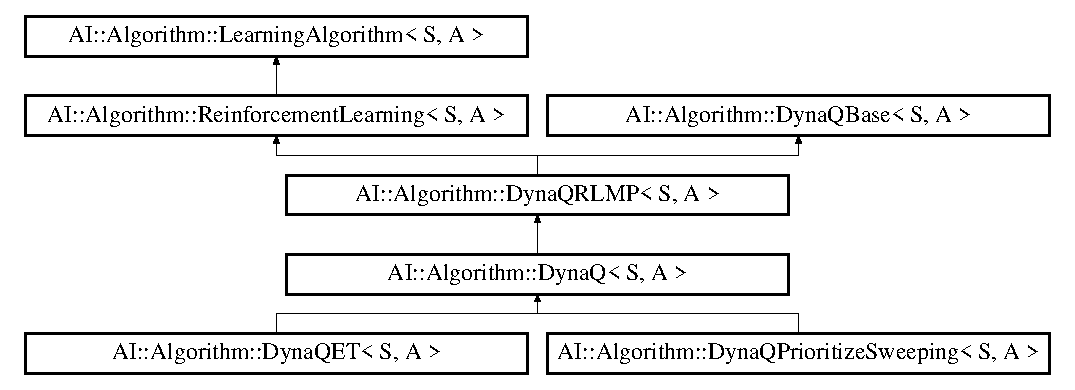
\includegraphics[height=4.794520cm]{classAI_1_1Algorithm_1_1DynaQ}
\end{center}
\end{figure}
\subsection*{Public Member Functions}
\begin{DoxyCompactItemize}
\item 
\hyperlink{classAI_1_1Algorithm_1_1DynaQ_a7a25f397835208cde0c975733873b76d}{Dyna\-Q} (A\-I\-::\-F\-L\-O\-A\-T step\-Size, A\-I\-::\-F\-L\-O\-A\-T discount\-Rate, \hyperlink{classAI_1_1Algorithm_1_1Policy}{Policy}$<$ S, A $>$ \&policy, A\-I\-::\-U\-I\-N\-T simulation\-Iteration\-Count, A\-I\-::\-F\-L\-O\-A\-T state\-Transition\-Greediness, A\-I\-::\-F\-L\-O\-A\-T state\-Transition\-Step\-Size)
\item 
virtual void \hyperlink{classAI_1_1Algorithm_1_1DynaQ_a4542226b17db4ed8a2c5ec17d37dc42f}{update} (const \hyperlink{classAI_1_1StateAction}{State\-Action}$<$ S, A $>$ \&current\-State\-Action, const S \&next\-State, const F\-L\-O\-A\-T reward, const set$<$ A $>$ \&action\-Set)
\end{DoxyCompactItemize}
\subsection*{Additional Inherited Members}


\subsection{Detailed Description}
\subsubsection*{template$<$class S, class A$>$class A\-I\-::\-Algorithm\-::\-Dyna\-Q$<$ S, A $>$}

\hyperlink{classAI_1_1Algorithm_1_1DynaQ}{Dyna\-Q} 

The \hyperlink{classAI_1_1Algorithm_1_1DynaQ}{Dyna\-Q} algorithm is a subclass of Reinforcement Algorithm. \hyperlink{classAI_1_1Algorithm_1_1DynaQ}{Dyna\-Q} employs simulation\-Count for every update thus improving the conversion rate.

\begin{DoxySeeAlso}{See Also}
\hyperlink{classAI_1_1StateActionTransition}{State\-Action\-Transition} representing the models. 
\end{DoxySeeAlso}


\subsection{Constructor \& Destructor Documentation}
\hypertarget{classAI_1_1Algorithm_1_1DynaQ_a7a25f397835208cde0c975733873b76d}{\index{A\-I\-::\-Algorithm\-::\-Dyna\-Q@{A\-I\-::\-Algorithm\-::\-Dyna\-Q}!Dyna\-Q@{Dyna\-Q}}
\index{Dyna\-Q@{Dyna\-Q}!AI::Algorithm::DynaQ@{A\-I\-::\-Algorithm\-::\-Dyna\-Q}}
\subsubsection[{Dyna\-Q}]{\setlength{\rightskip}{0pt plus 5cm}template$<$class S , class A $>$ {\bf A\-I\-::\-Algorithm\-::\-Dyna\-Q}$<$ S, A $>$\-::{\bf Dyna\-Q} (
\begin{DoxyParamCaption}
\item[{A\-I\-::\-F\-L\-O\-A\-T}]{step\-Size, }
\item[{A\-I\-::\-F\-L\-O\-A\-T}]{discount\-Rate, }
\item[{{\bf Policy}$<$ S, A $>$ \&}]{policy, }
\item[{A\-I\-::\-U\-I\-N\-T}]{simulation\-Iteration\-Count, }
\item[{A\-I\-::\-F\-L\-O\-A\-T}]{state\-Transition\-Greediness, }
\item[{A\-I\-::\-F\-L\-O\-A\-T}]{state\-Transition\-Step\-Size}
\end{DoxyParamCaption}
)}}\label{classAI_1_1Algorithm_1_1DynaQ_a7a25f397835208cde0c975733873b76d}

\begin{DoxyParams}{Parameters}
{\em step\-Size} & range \mbox{[}0.\-0, 1.\-0\mbox{]}. High step size means faster learning, but less precise convergence. \\
\hline
{\em discount\-Rate} & range \mbox{[}0.\-0, 1.\-0\mbox{]}. High discount rate means more consideration of future events. \\
\hline
{\em simulation\-Iteration\-Count} & How many simulation per update. \\
\hline
{\em state\-Transition\-Greediness} & High value means less likely to choose random action during simulation. \\
\hline
{\em state\-Transition\-Step\-Size} & High value means faster learning in models but lower values means more accurate models. \\
\hline
\end{DoxyParams}


\subsection{Member Function Documentation}
\hypertarget{classAI_1_1Algorithm_1_1DynaQ_a4542226b17db4ed8a2c5ec17d37dc42f}{\index{A\-I\-::\-Algorithm\-::\-Dyna\-Q@{A\-I\-::\-Algorithm\-::\-Dyna\-Q}!update@{update}}
\index{update@{update}!AI::Algorithm::DynaQ@{A\-I\-::\-Algorithm\-::\-Dyna\-Q}}
\subsubsection[{update}]{\setlength{\rightskip}{0pt plus 5cm}template$<$class S , class A $>$ void {\bf A\-I\-::\-Algorithm\-::\-Dyna\-Q}$<$ S, A $>$\-::update (
\begin{DoxyParamCaption}
\item[{const {\bf State\-Action}$<$ S, A $>$ \&}]{current\-State\-Action, }
\item[{const S \&}]{next\-State, }
\item[{const F\-L\-O\-A\-T}]{reward, }
\item[{const set$<$ A $>$ \&}]{action\-Set}
\end{DoxyParamCaption}
)\hspace{0.3cm}{\ttfamily [virtual]}}}\label{classAI_1_1Algorithm_1_1DynaQ_a4542226b17db4ed8a2c5ec17d37dc42f}
Update the state\-Action map. 
\begin{DoxyParams}{Parameters}
{\em current\-State} & \\
\hline
{\em current\-Action} & \\
\hline
{\em next\-State} & \\
\hline
{\em reward} & reward of current\-State and current\-Action. \\
\hline
{\em state\-Action} & A map of \hyperlink{classAI_1_1StateAction}{State\-Action} to Value. \\
\hline
{\em action\-Set} & A set of all actions. \\
\hline
\end{DoxyParams}
\begin{DoxyReturn}{Returns}
next action to be executed. 
\end{DoxyReturn}


Reimplemented from \hyperlink{classAI_1_1Algorithm_1_1ReinforcementLearning_a25d7fa245a79e61061436dc0f1db90cb}{A\-I\-::\-Algorithm\-::\-Reinforcement\-Learning$<$ S, A $>$}.



Reimplemented in \hyperlink{classAI_1_1Algorithm_1_1DynaQPrioritizeSweeping_ad08b55f3cf927189dd31abf9fc1c2959}{A\-I\-::\-Algorithm\-::\-Dyna\-Q\-Prioritize\-Sweeping$<$ S, A $>$}, and \hyperlink{classAI_1_1Algorithm_1_1DynaQETWatkins_aa4e40af0fd705cd5d1f7fd13834c57c6}{A\-I\-::\-Algorithm\-::\-Dyna\-Q\-E\-T\-Watkins$<$ S, A $>$}.



The documentation for this class was generated from the following file\-:\begin{DoxyCompactItemize}
\item 
Algorithms/\-Reinforcement\-Learning/Dyna\-Q.\-h\end{DoxyCompactItemize}

\hypertarget{classAI_1_1Algorithm_1_1DynaQBase}{\section{A\-I\-:\-:Algorithm\-:\-:Dyna\-Q\-Base$<$ S, A $>$ Class Template Reference}
\label{classAI_1_1Algorithm_1_1DynaQBase}\index{A\-I\-::\-Algorithm\-::\-Dyna\-Q\-Base$<$ S, A $>$@{A\-I\-::\-Algorithm\-::\-Dyna\-Q\-Base$<$ S, A $>$}}
}
Inheritance diagram for A\-I\-:\-:Algorithm\-:\-:Dyna\-Q\-Base$<$ S, A $>$\-:\begin{figure}[H]
\begin{center}
\leavevmode
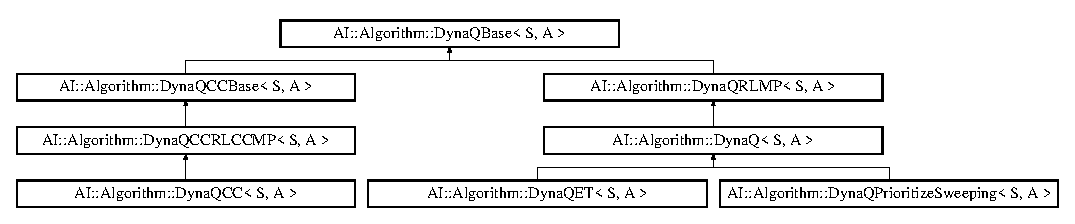
\includegraphics[height=2.557078cm]{classAI_1_1Algorithm_1_1DynaQBase}
\end{center}
\end{figure}
\subsection*{Public Member Functions}
\begin{DoxyCompactItemize}
\item 
\hypertarget{classAI_1_1Algorithm_1_1DynaQBase_a089f4024fab2f19179dea637b7f6c8ee}{{\bfseries Dyna\-Q\-Base} (\hyperlink{namespaceAI_ab6e14dc1e659854858a87e511f1439ec}{A\-I\-::\-U\-I\-N\-T} simulation\-Iteration\-Count, \hyperlink{namespaceAI_a41b74884a20833db653dded3918e05c3}{A\-I\-::\-F\-L\-O\-A\-T} state\-Transition\-Greediness, \hyperlink{namespaceAI_a41b74884a20833db653dded3918e05c3}{A\-I\-::\-F\-L\-O\-A\-T} state\-Transition\-Step\-Size)}\label{classAI_1_1Algorithm_1_1DynaQBase_a089f4024fab2f19179dea637b7f6c8ee}

\item 
\hypertarget{classAI_1_1Algorithm_1_1DynaQBase_a0d5777706e9c2be04ee1834ad593c795}{virtual void {\bfseries back\-Up\-State\-Action\-Pair} (const \hyperlink{classAI_1_1StateAction}{State\-Action}$<$ S, A $>$ \&current\-State\-Action, const \hyperlink{namespaceAI_a41b74884a20833db653dded3918e05c3}{F\-L\-O\-A\-T} reward, const \hyperlink{classAI_1_1StateAction}{State\-Action}$<$ S, A $>$ \&next\-State\-Action\-Pair)=0}\label{classAI_1_1Algorithm_1_1DynaQBase_a0d5777706e9c2be04ee1834ad593c795}

\item 
\hypertarget{classAI_1_1Algorithm_1_1DynaQBase_a32044f721ba4afbca5ea144b3f84135b}{virtual A {\bfseries arg\-Max} (const S \&state, const set$<$ A $>$ \&action\-Set) const =0}\label{classAI_1_1Algorithm_1_1DynaQBase_a32044f721ba4afbca5ea144b3f84135b}

\end{DoxyCompactItemize}
\subsection*{Protected Member Functions}
\begin{DoxyCompactItemize}
\item 
\hypertarget{classAI_1_1Algorithm_1_1DynaQBase_a4a45b9303a4b9e0cf93b9a5272739b35}{virtual void {\bfseries \-\_\-update\-Model} (const \hyperlink{classAI_1_1StateAction}{State\-Action}$<$ S, A $>$ \&current\-State\-Action, const S \&next\-State, const \hyperlink{namespaceAI_a41b74884a20833db653dded3918e05c3}{F\-L\-O\-A\-T} reward)}\label{classAI_1_1Algorithm_1_1DynaQBase_a4a45b9303a4b9e0cf93b9a5272739b35}

\item 
\hypertarget{classAI_1_1Algorithm_1_1DynaQBase_a0524b63604a75fd079b85a3a6e6ac93d}{virtual void {\bfseries \-\_\-add\-Model\-Safe} (const \hyperlink{classAI_1_1StateAction}{State\-Action}$<$ S, A $>$ \&current\-State\-Action)}\label{classAI_1_1Algorithm_1_1DynaQBase_a0524b63604a75fd079b85a3a6e6ac93d}

\item 
\hypertarget{classAI_1_1Algorithm_1_1DynaQBase_aefe879b3103a6c4f46176d9fcb1a911d}{virtual void {\bfseries \-\_\-add\-Model} (const \hyperlink{classAI_1_1StateAction}{State\-Action}$<$ S, A $>$ \&current\-State\-Action)}\label{classAI_1_1Algorithm_1_1DynaQBase_aefe879b3103a6c4f46176d9fcb1a911d}

\item 
\hypertarget{classAI_1_1Algorithm_1_1DynaQBase_ae33343ea87f96ee3a2c2651bfd2cbcc5}{virtual void {\bfseries \-\_\-simulate} (const set$<$ A $>$ \&action\-Set)}\label{classAI_1_1Algorithm_1_1DynaQBase_ae33343ea87f96ee3a2c2651bfd2cbcc5}

\end{DoxyCompactItemize}
\subsection*{Protected Attributes}
\begin{DoxyCompactItemize}
\item 
\hypertarget{classAI_1_1Algorithm_1_1DynaQBase_a3d375c3e01c7cc8a30c92109780adb9b}{\hyperlink{namespaceAI_ab6e14dc1e659854858a87e511f1439ec}{A\-I\-::\-U\-I\-N\-T} {\bfseries \-\_\-simulation\-Iteration\-Count}}\label{classAI_1_1Algorithm_1_1DynaQBase_a3d375c3e01c7cc8a30c92109780adb9b}

\item 
\hypertarget{classAI_1_1Algorithm_1_1DynaQBase_a1c9b96a2f0fa30d04d538b56ba008db4}{map$<$ \hyperlink{classAI_1_1StateAction}{State\-Action}$<$ S, A $>$\\*
, \hyperlink{classAI_1_1Algorithm_1_1StateActionTransition}{State\-Action\-Transition}$<$ S $>$ $>$ {\bfseries \-\_\-model}}\label{classAI_1_1Algorithm_1_1DynaQBase_a1c9b96a2f0fa30d04d538b56ba008db4}

\item 
\hypertarget{classAI_1_1Algorithm_1_1DynaQBase_ae3f83dbeea191fc8bdcd518a2e54af97}{\hyperlink{namespaceAI_a41b74884a20833db653dded3918e05c3}{A\-I\-::\-F\-L\-O\-A\-T} {\bfseries \-\_\-state\-Action\-Transition\-Greediness}}\label{classAI_1_1Algorithm_1_1DynaQBase_ae3f83dbeea191fc8bdcd518a2e54af97}

\item 
\hypertarget{classAI_1_1Algorithm_1_1DynaQBase_a1fd132ae0aeb356a891e5b81bf218338}{\hyperlink{namespaceAI_a41b74884a20833db653dded3918e05c3}{A\-I\-::\-F\-L\-O\-A\-T} {\bfseries \-\_\-state\-Action\-Transition\-Step\-Size}}\label{classAI_1_1Algorithm_1_1DynaQBase_a1fd132ae0aeb356a891e5b81bf218338}

\item 
\hypertarget{classAI_1_1Algorithm_1_1DynaQBase_adc3615604882454399863291f73b8734}{boost\-::shared\-\_\-mutex {\bfseries \-\_\-general\-Lock}}\label{classAI_1_1Algorithm_1_1DynaQBase_adc3615604882454399863291f73b8734}

\item 
\hypertarget{classAI_1_1Algorithm_1_1DynaQBase_ab166bd02d02f17c76a7626372c649849}{boost\-::shared\-\_\-mutex {\bfseries \-\_\-model\-Lock}}\label{classAI_1_1Algorithm_1_1DynaQBase_ab166bd02d02f17c76a7626372c649849}

\end{DoxyCompactItemize}


The documentation for this class was generated from the following file\-:\begin{DoxyCompactItemize}
\item 
Algorithms/\-Reinforcement\-Learning/Dyna\-Q\-Base.\-h\end{DoxyCompactItemize}

\hypertarget{classAI_1_1Algorithm_1_1DynaQCC}{\section{A\-I\-:\-:Algorithm\-:\-:Dyna\-Q\-C\-C$<$ S, A $>$ Class Template Reference}
\label{classAI_1_1Algorithm_1_1DynaQCC}\index{A\-I\-::\-Algorithm\-::\-Dyna\-Q\-C\-C$<$ S, A $>$@{A\-I\-::\-Algorithm\-::\-Dyna\-Q\-C\-C$<$ S, A $>$}}
}


\hyperlink{classAI_1_1Algorithm_1_1DynaQ}{Dyna\-Q} that performs simulation concurrently.  




{\ttfamily \#include $<$Dyna\-Q\-C\-C.\-h$>$}

Inheritance diagram for A\-I\-:\-:Algorithm\-:\-:Dyna\-Q\-C\-C$<$ S, A $>$\-:\begin{figure}[H]
\begin{center}
\leavevmode
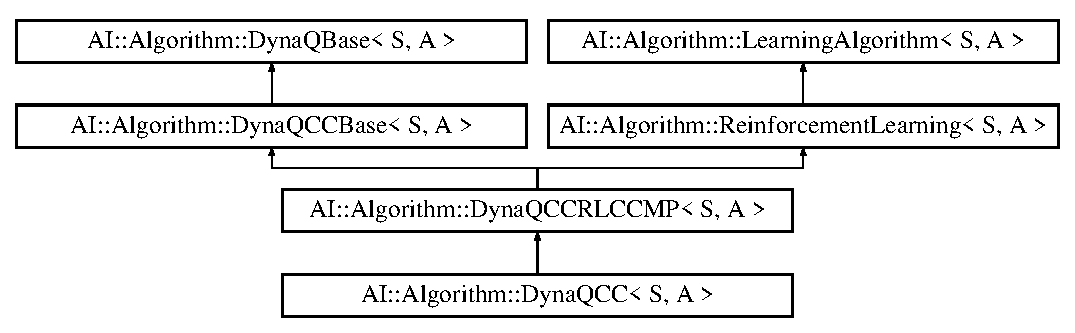
\includegraphics[height=4.000000cm]{classAI_1_1Algorithm_1_1DynaQCC}
\end{center}
\end{figure}
\subsection*{Public Member Functions}
\begin{DoxyCompactItemize}
\item 
\hyperlink{classAI_1_1Algorithm_1_1DynaQCC_aab347f88243e3690cbc856347ed37378}{Dyna\-Q\-C\-C} (\hyperlink{namespaceAI_a41b74884a20833db653dded3918e05c3}{A\-I\-::\-F\-L\-O\-A\-T} step\-Size, \hyperlink{namespaceAI_a41b74884a20833db653dded3918e05c3}{A\-I\-::\-F\-L\-O\-A\-T} discount\-Rate, \hyperlink{classAI_1_1Algorithm_1_1Policy_1_1Policy}{Policy\-::\-Policy}$<$ S, A $>$ \&policy, \hyperlink{namespaceAI_ab6e14dc1e659854858a87e511f1439ec}{A\-I\-::\-U\-I\-N\-T} simulation\-Iteration\-Count, \hyperlink{namespaceAI_a41b74884a20833db653dded3918e05c3}{A\-I\-::\-F\-L\-O\-A\-T} state\-Transition\-Greediness, \hyperlink{namespaceAI_a41b74884a20833db653dded3918e05c3}{A\-I\-::\-F\-L\-O\-A\-T} state\-Transition\-Step\-Size)
\item 
virtual void \hyperlink{classAI_1_1Algorithm_1_1DynaQCC_ae23b8f0afbb9fc5024aef9ce720c9b84}{update} (const \hyperlink{classAI_1_1StateAction}{State\-Action}$<$ S, A $>$ \&current\-State\-Action, const S \&next\-State, const \hyperlink{namespaceAI_a41b74884a20833db653dded3918e05c3}{F\-L\-O\-A\-T} reward, const set$<$ A $>$ \&action\-Set)
\end{DoxyCompactItemize}
\subsection*{Additional Inherited Members}


\subsection{Detailed Description}
\subsubsection*{template$<$class S, class A$>$class A\-I\-::\-Algorithm\-::\-Dyna\-Q\-C\-C$<$ S, A $>$}

\hyperlink{classAI_1_1Algorithm_1_1DynaQ}{Dyna\-Q} that performs simulation concurrently. 


\begin{DoxyTemplParams}{Template Parameters}
{\em S} & State data type. \\
\hline
{\em A} & Action data type.\\
\hline
\end{DoxyTemplParams}
\hyperlink{classAI_1_1Algorithm_1_1DynaQCC}{Dyna\-Q\-C\-C} must only be used when state space is large to take advantage of multi-\/threading. If state space is in order of thousands or more, \hyperlink{classAI_1_1Algorithm_1_1ReinforcementLearningGD}{Reinforcement\-Learning\-G\-D} might should be used. 

\subsection{Constructor \& Destructor Documentation}
\hypertarget{classAI_1_1Algorithm_1_1DynaQCC_aab347f88243e3690cbc856347ed37378}{\index{A\-I\-::\-Algorithm\-::\-Dyna\-Q\-C\-C@{A\-I\-::\-Algorithm\-::\-Dyna\-Q\-C\-C}!Dyna\-Q\-C\-C@{Dyna\-Q\-C\-C}}
\index{Dyna\-Q\-C\-C@{Dyna\-Q\-C\-C}!AI::Algorithm::DynaQCC@{A\-I\-::\-Algorithm\-::\-Dyna\-Q\-C\-C}}
\subsubsection[{Dyna\-Q\-C\-C}]{\setlength{\rightskip}{0pt plus 5cm}template$<$class S , class A $>$ {\bf A\-I\-::\-Algorithm\-::\-Dyna\-Q\-C\-C}$<$ S, A $>$\-::{\bf Dyna\-Q\-C\-C} (
\begin{DoxyParamCaption}
\item[{{\bf A\-I\-::\-F\-L\-O\-A\-T}}]{step\-Size, }
\item[{{\bf A\-I\-::\-F\-L\-O\-A\-T}}]{discount\-Rate, }
\item[{{\bf Policy\-::\-Policy}$<$ S, A $>$ \&}]{policy, }
\item[{{\bf A\-I\-::\-U\-I\-N\-T}}]{simulation\-Iteration\-Count, }
\item[{{\bf A\-I\-::\-F\-L\-O\-A\-T}}]{state\-Transition\-Greediness, }
\item[{{\bf A\-I\-::\-F\-L\-O\-A\-T}}]{state\-Transition\-Step\-Size}
\end{DoxyParamCaption}
)\hspace{0.3cm}{\ttfamily [inline]}}}\label{classAI_1_1Algorithm_1_1DynaQCC_aab347f88243e3690cbc856347ed37378}

\begin{DoxyParams}{Parameters}
{\em step\-Size} & range $[0.0, 1.0]$j. High step size means faster learning, but less precise convergence. \\
\hline
{\em discount\-Rate} & range $[0.0, 1.0]$. High discount rate means more consideration of future events. \\
\hline
{\em policy} & online policy, that is policy used for action selection. \\
\hline
{\em simulation\-Iteration\-Count} & number of simulations per update/backup. \\
\hline
{\em state\-Transition\-Greediness} & greediness in selecting highest value model. \\
\hline
{\em state\-Transition\-Step\-Size} & how fast does a model update a value of a state-\/action pair. \\
\hline
\end{DoxyParams}


\subsection{Member Function Documentation}
\hypertarget{classAI_1_1Algorithm_1_1DynaQCC_ae23b8f0afbb9fc5024aef9ce720c9b84}{\index{A\-I\-::\-Algorithm\-::\-Dyna\-Q\-C\-C@{A\-I\-::\-Algorithm\-::\-Dyna\-Q\-C\-C}!update@{update}}
\index{update@{update}!AI::Algorithm::DynaQCC@{A\-I\-::\-Algorithm\-::\-Dyna\-Q\-C\-C}}
\subsubsection[{update}]{\setlength{\rightskip}{0pt plus 5cm}template$<$class S , class A $>$ void {\bf A\-I\-::\-Algorithm\-::\-Dyna\-Q\-C\-C}$<$ S, A $>$\-::update (
\begin{DoxyParamCaption}
\item[{const {\bf State\-Action}$<$ S, A $>$ \&}]{current\-State\-Action, }
\item[{const S \&}]{next\-State, }
\item[{const {\bf F\-L\-O\-A\-T}}]{reward, }
\item[{const set$<$ A $>$ \&}]{action\-Set}
\end{DoxyParamCaption}
)\hspace{0.3cm}{\ttfamily [inline]}, {\ttfamily [virtual]}}}\label{classAI_1_1Algorithm_1_1DynaQCC_ae23b8f0afbb9fc5024aef9ce720c9b84}
Update the state\-Action map. 
\begin{DoxyParams}{Parameters}
{\em current\-State} & current\-State agent is in. \\
\hline
{\em current\-Action} & action taken by agent by being in current\-State. \\
\hline
{\em next\-State} & next\-State by taking current\-Action in current\-State. \\
\hline
{\em reward} & reward of current\-State\-Action. \\
\hline
{\em action\-Set} & A set of all actions. \\
\hline
\end{DoxyParams}


Reimplemented from \hyperlink{classAI_1_1Algorithm_1_1ReinforcementLearning_a25d7fa245a79e61061436dc0f1db90cb}{A\-I\-::\-Algorithm\-::\-Reinforcement\-Learning$<$ S, A $>$}.



The documentation for this class was generated from the following file\-:\begin{DoxyCompactItemize}
\item 
Algorithms/\-Reinforcement\-Learning/Dyna\-Q\-C\-C.\-h\end{DoxyCompactItemize}

\hypertarget{classAI_1_1Algorithm_1_1DynaQCCBase}{\section{A\-I\-:\-:Algorithm\-:\-:Dyna\-Q\-C\-C\-Base$<$ S, A $>$ Class Template Reference}
\label{classAI_1_1Algorithm_1_1DynaQCCBase}\index{A\-I\-::\-Algorithm\-::\-Dyna\-Q\-C\-C\-Base$<$ S, A $>$@{A\-I\-::\-Algorithm\-::\-Dyna\-Q\-C\-C\-Base$<$ S, A $>$}}
}
Inheritance diagram for A\-I\-:\-:Algorithm\-:\-:Dyna\-Q\-C\-C\-Base$<$ S, A $>$\-:\begin{figure}[H]
\begin{center}
\leavevmode
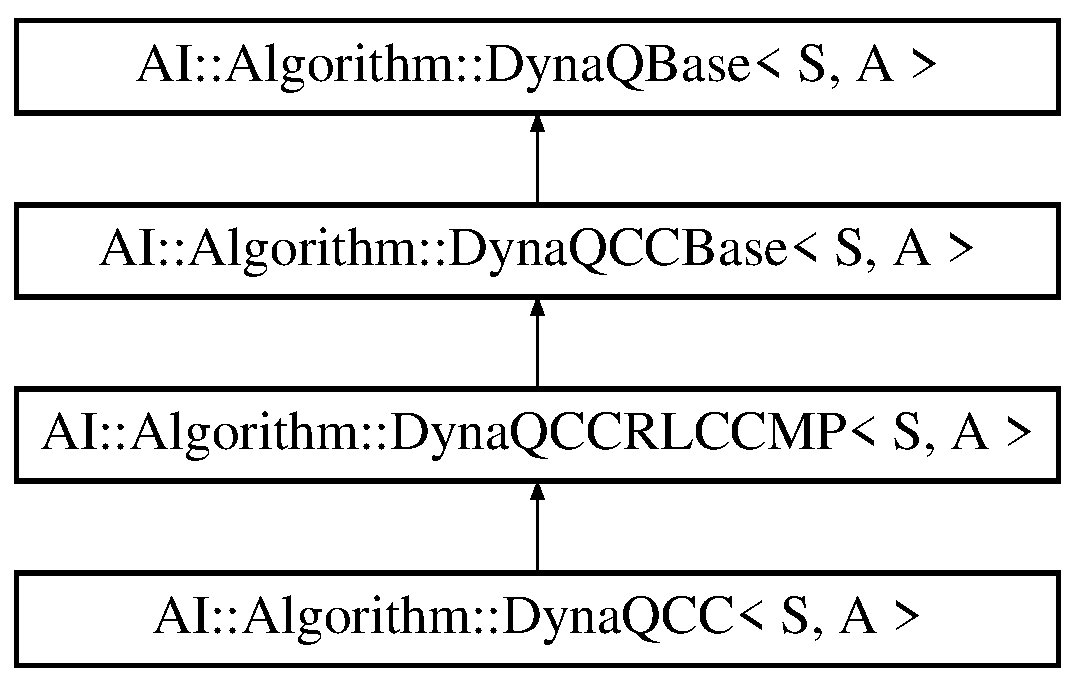
\includegraphics[height=4.000000cm]{classAI_1_1Algorithm_1_1DynaQCCBase}
\end{center}
\end{figure}
\subsection*{Public Member Functions}
\begin{DoxyCompactItemize}
\item 
\hypertarget{classAI_1_1Algorithm_1_1DynaQCCBase_acd1924d5f560d9a7298e442dfa33716a}{{\bfseries Dyna\-Q\-C\-C\-Base} (\hyperlink{namespaceAI_ab6e14dc1e659854858a87e511f1439ec}{A\-I\-::\-U\-I\-N\-T} simulation\-Iteration\-Count, \hyperlink{namespaceAI_a41b74884a20833db653dded3918e05c3}{A\-I\-::\-F\-L\-O\-A\-T} state\-Transition\-Greediness, \hyperlink{namespaceAI_a41b74884a20833db653dded3918e05c3}{A\-I\-::\-F\-L\-O\-A\-T} state\-Transition\-Step\-Size)}\label{classAI_1_1Algorithm_1_1DynaQCCBase_acd1924d5f560d9a7298e442dfa33716a}

\end{DoxyCompactItemize}
\subsection*{Protected Member Functions}
\begin{DoxyCompactItemize}
\item 
\hypertarget{classAI_1_1Algorithm_1_1DynaQCCBase_adc1bb07bb9025dc0c2963ded741b43a2}{virtual void {\bfseries \-\_\-simulate} (const set$<$ A $>$ \&action\-Set)}\label{classAI_1_1Algorithm_1_1DynaQCCBase_adc1bb07bb9025dc0c2963ded741b43a2}

\item 
\hypertarget{classAI_1_1Algorithm_1_1DynaQCCBase_a56e5d7ee46d67400f9e2411e801f93d2}{virtual void {\bfseries \-\_\-thread\-Worker} (const set$<$ A $>$ \&action\-Set, \hyperlink{namespaceAI_ab6e14dc1e659854858a87e511f1439ec}{A\-I\-::\-U\-I\-N\-T} local\-Simulation\-Steps)}\label{classAI_1_1Algorithm_1_1DynaQCCBase_a56e5d7ee46d67400f9e2411e801f93d2}

\item 
\hypertarget{classAI_1_1Algorithm_1_1DynaQCCBase_aeff65821d73179f84390892d8a2b0d3c}{void {\bfseries \-\_\-update\-Distribution} ()}\label{classAI_1_1Algorithm_1_1DynaQCCBase_aeff65821d73179f84390892d8a2b0d3c}

\end{DoxyCompactItemize}
\subsection*{Protected Attributes}
\begin{DoxyCompactItemize}
\item 
\hypertarget{classAI_1_1Algorithm_1_1DynaQCCBase_a0826c4c68c5d7b11bcb560d1b23b3252}{std\-::random\-\_\-device {\bfseries \-\_\-random\-Device}}\label{classAI_1_1Algorithm_1_1DynaQCCBase_a0826c4c68c5d7b11bcb560d1b23b3252}

\item 
\hypertarget{classAI_1_1Algorithm_1_1DynaQCCBase_ab2859ca39decdd0a8921e0ac500ed6f3}{std\-::uniform\-\_\-int\-\_\-distribution\\*
$<$ \hyperlink{namespaceAI_ac74584e573f07aa4194b461b1ba7be64}{A\-I\-::\-I\-N\-T} $>$ {\bfseries \-\_\-distribution}}\label{classAI_1_1Algorithm_1_1DynaQCCBase_ab2859ca39decdd0a8921e0ac500ed6f3}

\end{DoxyCompactItemize}


The documentation for this class was generated from the following file\-:\begin{DoxyCompactItemize}
\item 
Algorithms/\-Reinforcement\-Learning/Dyna\-Q\-C\-C\-Base.\-h\end{DoxyCompactItemize}

\hypertarget{classAI_1_1Algorithm_1_1DynaQCCRLCCMP}{\section{A\+I\+:\+:Algorithm\+:\+:Dyna\+Q\+C\+C\+R\+L\+C\+C\+M\+P$<$ S, A $>$ Class Template Reference}
\label{classAI_1_1Algorithm_1_1DynaQCCRLCCMP}\index{A\+I\+::\+Algorithm\+::\+Dyna\+Q\+C\+C\+R\+L\+C\+C\+M\+P$<$ S, A $>$@{A\+I\+::\+Algorithm\+::\+Dyna\+Q\+C\+C\+R\+L\+C\+C\+M\+P$<$ S, A $>$}}
}


Abstract/\+Base class for \hyperlink{classAI_1_1Algorithm_1_1DynaQCC}{Dyna\+Q\+C\+C} algorithm.  




{\ttfamily \#include $<$Dyna\+Q\+C\+C\+R\+L\+C\+C\+M\+P.\+h$>$}

Inheritance diagram for A\+I\+:\+:Algorithm\+:\+:Dyna\+Q\+C\+C\+R\+L\+C\+C\+M\+P$<$ S, A $>$\+:\begin{figure}[H]
\begin{center}
\leavevmode
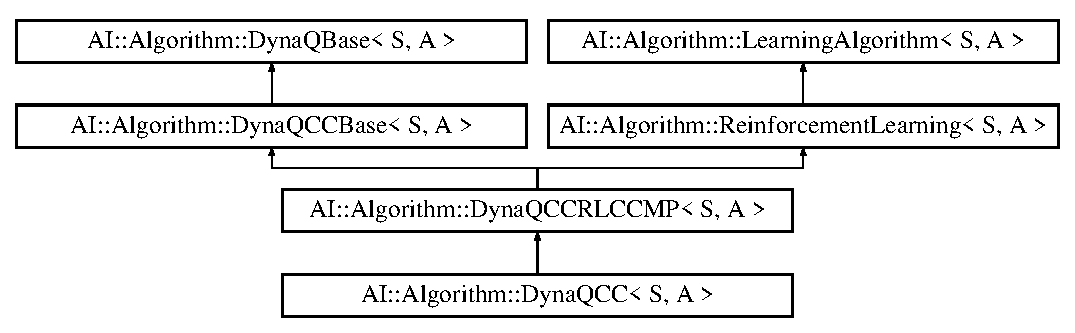
\includegraphics[height=4.000000cm]{classAI_1_1Algorithm_1_1DynaQCCRLCCMP}
\end{center}
\end{figure}
\subsection*{Public Member Functions}
\begin{DoxyCompactItemize}
\item 
\hyperlink{classAI_1_1Algorithm_1_1DynaQCCRLCCMP_a892dd156f280dd375d7f248258531043}{Dyna\+Q\+C\+C\+R\+L\+C\+C\+M\+P} (\hyperlink{namespaceAI_a41b74884a20833db653dded3918e05c3}{A\+I\+::\+F\+L\+O\+A\+T} step\+Size, \hyperlink{namespaceAI_a41b74884a20833db653dded3918e05c3}{A\+I\+::\+F\+L\+O\+A\+T} discount\+Rate, \hyperlink{classAI_1_1Algorithm_1_1Policy_1_1Policy}{Policy\+::\+Policy}$<$ S, A $>$ \&policy, \hyperlink{namespaceAI_ab6e14dc1e659854858a87e511f1439ec}{A\+I\+::\+U\+I\+N\+T} simulation\+Iteration\+Count, \hyperlink{namespaceAI_a41b74884a20833db653dded3918e05c3}{A\+I\+::\+F\+L\+O\+A\+T} state\+Transition\+Greediness, \hyperlink{namespaceAI_a41b74884a20833db653dded3918e05c3}{A\+I\+::\+F\+L\+O\+A\+T} state\+Transition\+Step\+Size)
\item 
virtual void \hyperlink{classAI_1_1Algorithm_1_1DynaQCCRLCCMP_aebff9b81db5bd2ae33bd3d6662539bc0}{back\+Up\+State\+Action\+Pair} (const \hyperlink{classAI_1_1StateAction}{State\+Action}$<$ S, A $>$ \&current\+State\+Action, const \hyperlink{namespaceAI_a41b74884a20833db653dded3918e05c3}{F\+L\+O\+A\+T} reward, const \hyperlink{classAI_1_1StateAction}{State\+Action}$<$ S, A $>$ \&next\+State\+Action\+Pair)
\item 
virtual A \hyperlink{classAI_1_1Algorithm_1_1DynaQCCRLCCMP_a145fa4fdba2289842a77c9d483a42ef2}{arg\+Max} (const S \&state, const set$<$ A $>$ \&action\+Set) const 
\end{DoxyCompactItemize}
\subsection*{Additional Inherited Members}


\subsection{Detailed Description}
\subsubsection*{template$<$class S, class A$>$class A\+I\+::\+Algorithm\+::\+Dyna\+Q\+C\+C\+R\+L\+C\+C\+M\+P$<$ S, A $>$}

Abstract/\+Base class for \hyperlink{classAI_1_1Algorithm_1_1DynaQCC}{Dyna\+Q\+C\+C} algorithm. 


\begin{DoxyTemplParams}{Template Parameters}
{\em S} & State data type. \\
\hline
{\em A} & Action data type.\\
\hline
\end{DoxyTemplParams}
Merge point for \hyperlink{classAI_1_1Algorithm_1_1DynaQCC}{Dyna\+Q\+C\+C} and Reinforcement Learning. 

\subsection{Constructor \& Destructor Documentation}
\hypertarget{classAI_1_1Algorithm_1_1DynaQCCRLCCMP_a892dd156f280dd375d7f248258531043}{\index{A\+I\+::\+Algorithm\+::\+Dyna\+Q\+C\+C\+R\+L\+C\+C\+M\+P@{A\+I\+::\+Algorithm\+::\+Dyna\+Q\+C\+C\+R\+L\+C\+C\+M\+P}!Dyna\+Q\+C\+C\+R\+L\+C\+C\+M\+P@{Dyna\+Q\+C\+C\+R\+L\+C\+C\+M\+P}}
\index{Dyna\+Q\+C\+C\+R\+L\+C\+C\+M\+P@{Dyna\+Q\+C\+C\+R\+L\+C\+C\+M\+P}!A\+I\+::\+Algorithm\+::\+Dyna\+Q\+C\+C\+R\+L\+C\+C\+M\+P@{A\+I\+::\+Algorithm\+::\+Dyna\+Q\+C\+C\+R\+L\+C\+C\+M\+P}}
\subsubsection[{Dyna\+Q\+C\+C\+R\+L\+C\+C\+M\+P}]{\setlength{\rightskip}{0pt plus 5cm}template$<$class S , class A $>$ {\bf A\+I\+::\+Algorithm\+::\+Dyna\+Q\+C\+C\+R\+L\+C\+C\+M\+P}$<$ S, A $>$\+::{\bf Dyna\+Q\+C\+C\+R\+L\+C\+C\+M\+P} (
\begin{DoxyParamCaption}
\item[{{\bf A\+I\+::\+F\+L\+O\+A\+T}}]{step\+Size, }
\item[{{\bf A\+I\+::\+F\+L\+O\+A\+T}}]{discount\+Rate, }
\item[{{\bf Policy\+::\+Policy}$<$ S, A $>$ \&}]{policy, }
\item[{{\bf A\+I\+::\+U\+I\+N\+T}}]{simulation\+Iteration\+Count, }
\item[{{\bf A\+I\+::\+F\+L\+O\+A\+T}}]{state\+Transition\+Greediness, }
\item[{{\bf A\+I\+::\+F\+L\+O\+A\+T}}]{state\+Transition\+Step\+Size}
\end{DoxyParamCaption}
)\hspace{0.3cm}{\ttfamily [inline]}}}\label{classAI_1_1Algorithm_1_1DynaQCCRLCCMP_a892dd156f280dd375d7f248258531043}

\begin{DoxyParams}{Parameters}
{\em step\+Size} & range $[0.0, 1.0]$j. High step size means faster learning, but less precise convergence. \\
\hline
{\em discount\+Rate} & range $[0.0, 1.0]$. High discount rate means more consideration of future events. \\
\hline
{\em policy} & online policy, that is policy used for action selection. \\
\hline
{\em simulation\+Iteration\+Count} & number of simulations per update/backup. \\
\hline
{\em state\+Transition\+Greediness} & greediness in selecting highest value model. \\
\hline
{\em state\+Transition\+Step\+Size} & how fast does a model update a value of a state-\/action pair. \\
\hline
\end{DoxyParams}


\subsection{Member Function Documentation}
\hypertarget{classAI_1_1Algorithm_1_1DynaQCCRLCCMP_a145fa4fdba2289842a77c9d483a42ef2}{\index{A\+I\+::\+Algorithm\+::\+Dyna\+Q\+C\+C\+R\+L\+C\+C\+M\+P@{A\+I\+::\+Algorithm\+::\+Dyna\+Q\+C\+C\+R\+L\+C\+C\+M\+P}!arg\+Max@{arg\+Max}}
\index{arg\+Max@{arg\+Max}!A\+I\+::\+Algorithm\+::\+Dyna\+Q\+C\+C\+R\+L\+C\+C\+M\+P@{A\+I\+::\+Algorithm\+::\+Dyna\+Q\+C\+C\+R\+L\+C\+C\+M\+P}}
\subsubsection[{arg\+Max}]{\setlength{\rightskip}{0pt plus 5cm}template$<$class S , class A $>$ A {\bf A\+I\+::\+Algorithm\+::\+Dyna\+Q\+C\+C\+R\+L\+C\+C\+M\+P}$<$ S, A $>$\+::arg\+Max (
\begin{DoxyParamCaption}
\item[{const S \&}]{state, }
\item[{const set$<$ A $>$ \&}]{action\+Set}
\end{DoxyParamCaption}
) const\hspace{0.3cm}{\ttfamily [inline]}, {\ttfamily [virtual]}}}\label{classAI_1_1Algorithm_1_1DynaQCCRLCCMP_a145fa4fdba2289842a77c9d483a42ef2}
Note that this is just a place-\/holder, since this will be aggregate arg\+Max implementations in children. Returns the action that will most \char`\"{}likely\char`\"{} gives the highest reward from the current state. 
\begin{DoxyParams}{Parameters}
{\em state} & the state to apply the arg\+Max to. \\
\hline
{\em state\+Action} & map of \hyperlink{classAI_1_1StateAction}{State\+Action} to value. \\
\hline
{\em action\+Set} & a set of possible actions. \\
\hline
\end{DoxyParams}
\begin{DoxyReturn}{Returns}
the action that will \char`\"{}likely\char`\"{} gives the highest reward. 
\end{DoxyReturn}


Implements \hyperlink{classAI_1_1Algorithm_1_1DynaQBase_a32044f721ba4afbca5ea144b3f84135b}{A\+I\+::\+Algorithm\+::\+Dyna\+Q\+Base$<$ S, A $>$}.

\hypertarget{classAI_1_1Algorithm_1_1DynaQCCRLCCMP_aebff9b81db5bd2ae33bd3d6662539bc0}{\index{A\+I\+::\+Algorithm\+::\+Dyna\+Q\+C\+C\+R\+L\+C\+C\+M\+P@{A\+I\+::\+Algorithm\+::\+Dyna\+Q\+C\+C\+R\+L\+C\+C\+M\+P}!back\+Up\+State\+Action\+Pair@{back\+Up\+State\+Action\+Pair}}
\index{back\+Up\+State\+Action\+Pair@{back\+Up\+State\+Action\+Pair}!A\+I\+::\+Algorithm\+::\+Dyna\+Q\+C\+C\+R\+L\+C\+C\+M\+P@{A\+I\+::\+Algorithm\+::\+Dyna\+Q\+C\+C\+R\+L\+C\+C\+M\+P}}
\subsubsection[{back\+Up\+State\+Action\+Pair}]{\setlength{\rightskip}{0pt plus 5cm}template$<$class S , class A $>$ void {\bf A\+I\+::\+Algorithm\+::\+Dyna\+Q\+C\+C\+R\+L\+C\+C\+M\+P}$<$ S, A $>$\+::back\+Up\+State\+Action\+Pair (
\begin{DoxyParamCaption}
\item[{const {\bf State\+Action}$<$ S, A $>$ \&}]{current\+State\+Action, }
\item[{const {\bf F\+L\+O\+A\+T}}]{reward, }
\item[{const {\bf State\+Action}$<$ S, A $>$ \&}]{next\+State\+Action\+Pair}
\end{DoxyParamCaption}
)\hspace{0.3cm}{\ttfamily [inline]}, {\ttfamily [virtual]}}}\label{classAI_1_1Algorithm_1_1DynaQCCRLCCMP_aebff9b81db5bd2ae33bd3d6662539bc0}
Does the main back up for all Temporal difference\+: $ Q[S, A] \leftarrow Q[S, A] + \alpha\times [R + \gamma \times max_{A'}Q[S', A'] - Q[S, A] ]$ 
\begin{DoxyParams}{Parameters}
{\em current\+State\+Action} & $(S, A)$, current state-\/action pair. \\
\hline
{\em reward} & $R$, reward after $(S, A)$. \\
\hline
{\em next\+State\+Action\+Pair} & $(S', A')$, next state-\/action pair. \\
\hline
\end{DoxyParams}


Reimplemented from \hyperlink{classAI_1_1Algorithm_1_1ReinforcementLearning_aa45b49ec954f6934df4d541b70076bd6}{A\+I\+::\+Algorithm\+::\+Reinforcement\+Learning$<$ S, A $>$}.



The documentation for this class was generated from the following file\+:\begin{DoxyCompactItemize}
\item 
Algorithms/\+Reinforcement\+Learning/Dyna\+Q\+C\+C\+R\+L\+C\+C\+M\+P.\+h\end{DoxyCompactItemize}

\hypertarget{classAI_1_1Algorithm_1_1DynaQETWatkins}{\section{A\-I\-:\-:Algorithm\-:\-:Dyna\-Q\-E\-T\-Watkins$<$ S, A $>$ Class Template Reference}
\label{classAI_1_1Algorithm_1_1DynaQETWatkins}\index{A\-I\-::\-Algorithm\-::\-Dyna\-Q\-E\-T\-Watkins$<$ S, A $>$@{A\-I\-::\-Algorithm\-::\-Dyna\-Q\-E\-T\-Watkins$<$ S, A $>$}}
}


Employs the simulation of \hyperlink{classAI_1_1Algorithm_1_1DynaQ}{Dyna\-Q} plus eligibility traces.  




{\ttfamily \#include $<$Dyna\-Q\-E\-T\-Watkins.\-h$>$}

Inheritance diagram for A\-I\-:\-:Algorithm\-:\-:Dyna\-Q\-E\-T\-Watkins$<$ S, A $>$\-:\begin{figure}[H]
\begin{center}
\leavevmode
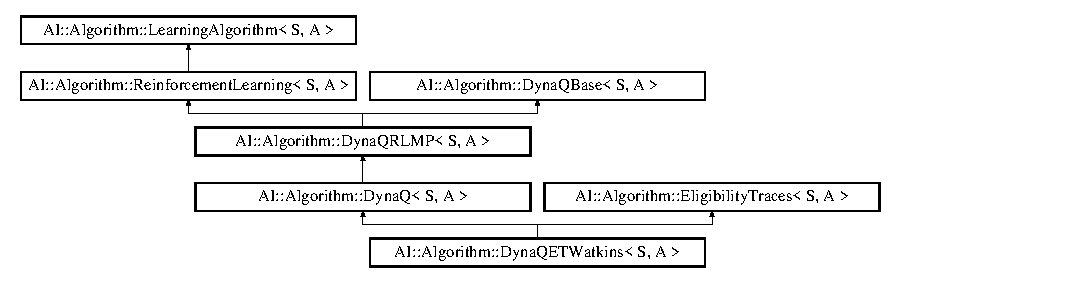
\includegraphics[height=3.357314cm]{classAI_1_1Algorithm_1_1DynaQETWatkins}
\end{center}
\end{figure}
\subsection*{Public Member Functions}
\begin{DoxyCompactItemize}
\item 
\hyperlink{classAI_1_1Algorithm_1_1DynaQETWatkins_a0601ab5adb8ba7d0d94d93b6194528c9}{Dyna\-Q\-E\-T\-Watkins} (\hyperlink{namespaceAI_a41b74884a20833db653dded3918e05c3}{A\-I\-::\-F\-L\-O\-A\-T} step\-Size, \hyperlink{namespaceAI_a41b74884a20833db653dded3918e05c3}{A\-I\-::\-F\-L\-O\-A\-T} discount\-Rate, \hyperlink{classAI_1_1Algorithm_1_1Policy_1_1Policy}{Policy\-::\-Policy}$<$ S, A $>$ \&policy, \hyperlink{namespaceAI_ab6e14dc1e659854858a87e511f1439ec}{A\-I\-::\-U\-I\-N\-T} simulation\-Iteration\-Count, \hyperlink{namespaceAI_a41b74884a20833db653dded3918e05c3}{A\-I\-::\-F\-L\-O\-A\-T} state\-Transition\-Greediness, \hyperlink{namespaceAI_a41b74884a20833db653dded3918e05c3}{A\-I\-::\-F\-L\-O\-A\-T} state\-Transition\-Step\-Size, \hyperlink{namespaceAI_a41b74884a20833db653dded3918e05c3}{A\-I\-::\-F\-L\-O\-A\-T} lambda)
\item 
virtual void \hyperlink{classAI_1_1Algorithm_1_1DynaQETWatkins_aa4e40af0fd705cd5d1f7fd13834c57c6}{update} (const \hyperlink{classAI_1_1StateAction}{State\-Action}$<$ S, A $>$ \&current\-State\-Action, const S \&next\-State, const \hyperlink{namespaceAI_a41b74884a20833db653dded3918e05c3}{A\-I\-::\-F\-L\-O\-A\-T} current\-State\-Action\-Value, const set$<$ A $>$ \&action\-Set)
\end{DoxyCompactItemize}
\subsection*{Additional Inherited Members}


\subsection{Detailed Description}
\subsubsection*{template$<$class S, class A$>$class A\-I\-::\-Algorithm\-::\-Dyna\-Q\-E\-T\-Watkins$<$ S, A $>$}

Employs the simulation of \hyperlink{classAI_1_1Algorithm_1_1DynaQ}{Dyna\-Q} plus eligibility traces. 

Like \hyperlink{classAI_1_1Algorithm_1_1DynaQ}{Dyna\-Q}, it does $n$ simlations per update, but after than performs eligibility traces.

\begin{DoxySeeAlso}{See Also}
\hyperlink{classAI_1_1Algorithm_1_1DynaQ}{Dyna\-Q} 

\hyperlink{classAI_1_1Algorithm_1_1EligibilityTraces}{Eligibility\-Traces} 
\end{DoxySeeAlso}


\subsection{Constructor \& Destructor Documentation}
\hypertarget{classAI_1_1Algorithm_1_1DynaQETWatkins_a0601ab5adb8ba7d0d94d93b6194528c9}{\index{A\-I\-::\-Algorithm\-::\-Dyna\-Q\-E\-T\-Watkins@{A\-I\-::\-Algorithm\-::\-Dyna\-Q\-E\-T\-Watkins}!Dyna\-Q\-E\-T\-Watkins@{Dyna\-Q\-E\-T\-Watkins}}
\index{Dyna\-Q\-E\-T\-Watkins@{Dyna\-Q\-E\-T\-Watkins}!AI::Algorithm::DynaQETWatkins@{A\-I\-::\-Algorithm\-::\-Dyna\-Q\-E\-T\-Watkins}}
\subsubsection[{Dyna\-Q\-E\-T\-Watkins}]{\setlength{\rightskip}{0pt plus 5cm}template$<$class S , class A $>$ {\bf A\-I\-::\-Algorithm\-::\-Dyna\-Q\-E\-T\-Watkins}$<$ S, A $>$\-::{\bf Dyna\-Q\-E\-T\-Watkins} (
\begin{DoxyParamCaption}
\item[{{\bf A\-I\-::\-F\-L\-O\-A\-T}}]{step\-Size, }
\item[{{\bf A\-I\-::\-F\-L\-O\-A\-T}}]{discount\-Rate, }
\item[{{\bf Policy\-::\-Policy}$<$ S, A $>$ \&}]{policy, }
\item[{{\bf A\-I\-::\-U\-I\-N\-T}}]{simulation\-Iteration\-Count, }
\item[{{\bf A\-I\-::\-F\-L\-O\-A\-T}}]{state\-Transition\-Greediness, }
\item[{{\bf A\-I\-::\-F\-L\-O\-A\-T}}]{state\-Transition\-Step\-Size, }
\item[{{\bf A\-I\-::\-F\-L\-O\-A\-T}}]{lambda}
\end{DoxyParamCaption}
)}}\label{classAI_1_1Algorithm_1_1DynaQETWatkins_a0601ab5adb8ba7d0d94d93b6194528c9}

\begin{DoxyParams}{Parameters}
{\em step\-Size} & range $[0.0, 1.0]$. High step size means faster learning, but less precise convergence. \\
\hline
{\em discount\-Rate} & range $[0.0, 1.0]$. High discount rate means more consideration of future events. \\
\hline
{\em policy} & online policy, that is policy used for action selection. \\
\hline
{\em simulation\-Iteration\-Count} & number of simulations per update/backup. \\
\hline
{\em state\-Transition\-Greediness} & greediness in selecting highest value model. \\
\hline
{\em state\-Transition\-Step\-Size} & how fast does a model update a value of a state-\/action pair. \\
\hline
{\em lambda} & huge $\lambda$ means basically back up ranging from terminal state to initial state. Small $\lambda$ converges to T\-D(0). \\
\hline
\end{DoxyParams}


\subsection{Member Function Documentation}
\hypertarget{classAI_1_1Algorithm_1_1DynaQETWatkins_aa4e40af0fd705cd5d1f7fd13834c57c6}{\index{A\-I\-::\-Algorithm\-::\-Dyna\-Q\-E\-T\-Watkins@{A\-I\-::\-Algorithm\-::\-Dyna\-Q\-E\-T\-Watkins}!update@{update}}
\index{update@{update}!AI::Algorithm::DynaQETWatkins@{A\-I\-::\-Algorithm\-::\-Dyna\-Q\-E\-T\-Watkins}}
\subsubsection[{update}]{\setlength{\rightskip}{0pt plus 5cm}template$<$class S , class A $>$ void {\bf A\-I\-::\-Algorithm\-::\-Dyna\-Q\-E\-T\-Watkins}$<$ S, A $>$\-::update (
\begin{DoxyParamCaption}
\item[{const {\bf State\-Action}$<$ S, A $>$ \&}]{current\-State\-Action, }
\item[{const S \&}]{next\-State, }
\item[{const {\bf A\-I\-::\-F\-L\-O\-A\-T}}]{reward, }
\item[{const set$<$ A $>$ \&}]{action\-Set}
\end{DoxyParamCaption}
)\hspace{0.3cm}{\ttfamily [virtual]}}}\label{classAI_1_1Algorithm_1_1DynaQETWatkins_aa4e40af0fd705cd5d1f7fd13834c57c6}
Update the state\-Action map. 
\begin{DoxyParams}{Parameters}
{\em current\-State} & current\-State agent is in. \\
\hline
{\em current\-Action} & action taken by agent by being in current\-State. \\
\hline
{\em next\-State} & next\-State by taking current\-Action in current\-State. \\
\hline
{\em reward} & reward of current\-State\-Action. \\
\hline
{\em action\-Set} & A set of all actions. \\
\hline
\end{DoxyParams}


Reimplemented from \hyperlink{classAI_1_1Algorithm_1_1DynaQ_a4542226b17db4ed8a2c5ec17d37dc42f}{A\-I\-::\-Algorithm\-::\-Dyna\-Q$<$ S, A $>$}.



The documentation for this class was generated from the following file\-:\begin{DoxyCompactItemize}
\item 
Algorithms/\-Reinforcement\-Learning/Dyna\-Q\-E\-T\-Watkins.\-h\end{DoxyCompactItemize}

\hypertarget{classDynaQPlus}{\section{Dyna\-Q\-Plus Class Reference}
\label{classDynaQPlus}\index{Dyna\-Q\-Plus@{Dyna\-Q\-Plus}}
}


The documentation for this class was generated from the following file\-:\begin{DoxyCompactItemize}
\item 
Algorithms/\-Reinforcement\-Learning/Dyna\-Q\-Plus.\-h\end{DoxyCompactItemize}

\hypertarget{classAI_1_1Algorithm_1_1DynaQPrioritizeSweeping}{\section{A\-I\-:\-:Algorithm\-:\-:Dyna\-Q\-Prioritize\-Sweeping$<$ S, A $>$ Class Template Reference}
\label{classAI_1_1Algorithm_1_1DynaQPrioritizeSweeping}\index{A\-I\-::\-Algorithm\-::\-Dyna\-Q\-Prioritize\-Sweeping$<$ S, A $>$@{A\-I\-::\-Algorithm\-::\-Dyna\-Q\-Prioritize\-Sweeping$<$ S, A $>$}}
}


{\ttfamily \#include $<$Dyna\-Q\-Prioritized\-Sweeping.\-h$>$}

Inheritance diagram for A\-I\-:\-:Algorithm\-:\-:Dyna\-Q\-Prioritize\-Sweeping$<$ S, A $>$\-:\begin{figure}[H]
\begin{center}
\leavevmode
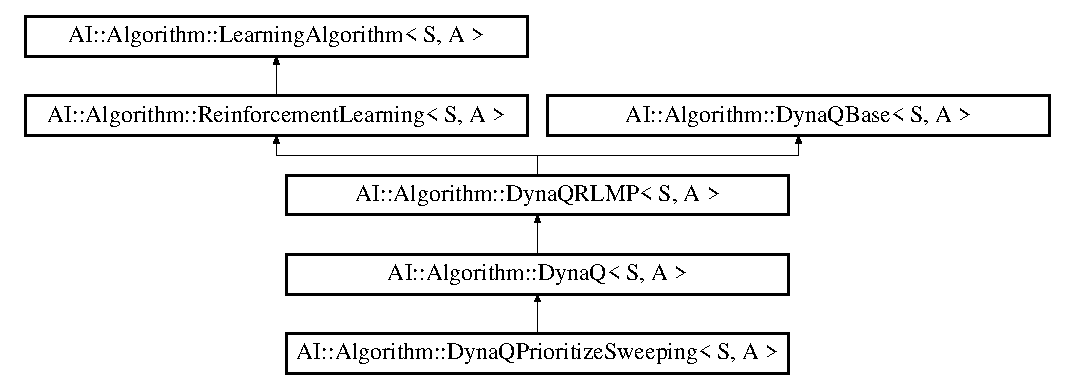
\includegraphics[height=4.794520cm]{classAI_1_1Algorithm_1_1DynaQPrioritizeSweeping}
\end{center}
\end{figure}
\subsection*{Public Member Functions}
\begin{DoxyCompactItemize}
\item 
\hyperlink{classAI_1_1Algorithm_1_1DynaQPrioritizeSweeping_ac1b32e8772e967a3bb74ac34708e4dfe}{Dyna\-Q\-Prioritize\-Sweeping} (\hyperlink{namespaceAI_a41b74884a20833db653dded3918e05c3}{A\-I\-::\-F\-L\-O\-A\-T} step\-Size, \hyperlink{namespaceAI_a41b74884a20833db653dded3918e05c3}{A\-I\-::\-F\-L\-O\-A\-T} discount\-Rate, \hyperlink{classAI_1_1Algorithm_1_1Policy_1_1Policy}{Policy\-::\-Policy}$<$ S, A $>$ \&policy, \hyperlink{namespaceAI_ab6e14dc1e659854858a87e511f1439ec}{A\-I\-::\-U\-I\-N\-T} simulation\-Iteration\-Count, \hyperlink{namespaceAI_a41b74884a20833db653dded3918e05c3}{A\-I\-::\-F\-L\-O\-A\-T} state\-Transition\-Greediness, \hyperlink{namespaceAI_a41b74884a20833db653dded3918e05c3}{A\-I\-::\-F\-L\-O\-A\-T} state\-Transition\-Step\-Size, \hyperlink{namespaceAI_a41b74884a20833db653dded3918e05c3}{A\-I\-::\-F\-L\-O\-A\-T} priority\-Threshold)
\item 
virtual void \hyperlink{classAI_1_1Algorithm_1_1DynaQPrioritizeSweeping_ad08b55f3cf927189dd31abf9fc1c2959}{update} (const \hyperlink{classAI_1_1StateAction}{State\-Action}$<$ S, A $>$ \&current\-State\-Action, const S \&next\-State, const \hyperlink{namespaceAI_a41b74884a20833db653dded3918e05c3}{A\-I\-::\-F\-L\-O\-A\-T} reward, const set$<$ A $>$ \&action\-Set)
\end{DoxyCompactItemize}
\subsection*{Protected Member Functions}
\begin{DoxyCompactItemize}
\item 
\hypertarget{classAI_1_1Algorithm_1_1DynaQPrioritizeSweeping_a328421d2cc8ad26641b7786a5ca8b640}{void {\bfseries \-\_\-priority\-Sweep} (const set$<$ A $>$ \&action\-Set)}\label{classAI_1_1Algorithm_1_1DynaQPrioritizeSweeping_a328421d2cc8ad26641b7786a5ca8b640}

\item 
\hypertarget{classAI_1_1Algorithm_1_1DynaQPrioritizeSweeping_a9f69f4ed43b2d9bdb446241fffbb20d7}{\hyperlink{namespaceAI_a41b74884a20833db653dded3918e05c3}{A\-I\-::\-F\-L\-O\-A\-T} {\bfseries \-\_\-get\-T\-D\-Error} (const \hyperlink{classAI_1_1StateAction}{State\-Action}$<$ S, A $>$ \&current\-State\-Action, const \hyperlink{namespaceAI_a41b74884a20833db653dded3918e05c3}{A\-I\-::\-F\-L\-O\-A\-T} reward, const \hyperlink{classAI_1_1StateAction}{State\-Action}$<$ S, A $>$ \&next\-State\-Action)}\label{classAI_1_1Algorithm_1_1DynaQPrioritizeSweeping_a9f69f4ed43b2d9bdb446241fffbb20d7}

\end{DoxyCompactItemize}
\subsection*{Protected Attributes}
\begin{DoxyCompactItemize}
\item 
\hypertarget{classAI_1_1Algorithm_1_1DynaQPrioritizeSweeping_aceb5ef5c47db0d322b4e03ec2c457d1a}{priority\-\_\-queue\\*
$<$ State\-Action\-Pair, std\-::vector\\*
$<$ State\-Action\-Pair $>$\\*
, \hyperlink{classAI_1_1StateActionPairValueComparison}{State\-Action\-Pair\-Value\-Comparison}\\*
$<$ S, A $>$ $>$ {\bfseries \-\_\-priority\-Queue}}\label{classAI_1_1Algorithm_1_1DynaQPrioritizeSweeping_aceb5ef5c47db0d322b4e03ec2c457d1a}

\item 
\hypertarget{classAI_1_1Algorithm_1_1DynaQPrioritizeSweeping_adc3809217aba2de41fbea2b9fb9e5648}{\hyperlink{namespaceAI_a41b74884a20833db653dded3918e05c3}{A\-I\-::\-F\-L\-O\-A\-T} {\bfseries \-\_\-priority\-Threshold}}\label{classAI_1_1Algorithm_1_1DynaQPrioritizeSweeping_adc3809217aba2de41fbea2b9fb9e5648}

\end{DoxyCompactItemize}
\subsection*{Additional Inherited Members}


\subsection{Detailed Description}
\subsubsection*{template$<$class S, class A$>$class A\-I\-::\-Algorithm\-::\-Dyna\-Q\-Prioritize\-Sweeping$<$ S, A $>$}

\hyperlink{classAI_1_1Algorithm_1_1DynaQPrioritizeSweeping}{Dyna\-Q\-Prioritize\-Sweeping} 

Prioritize Sweeping only backs up states that factor the most to achieving the goal during simulation. This way convergence is achieve faster. Very useful in large state spaces.

\begin{DoxyNote}{Note}
This is currently very slow. An update is being cultivated.
\end{DoxyNote}
\begin{DoxySeeAlso}{See Also}
\hyperlink{classAI_1_1Algorithm_1_1StateActionTransition}{State\-Action\-Transition} representing the models.

\hyperlink{classAI_1_1Algorithm_1_1DynaQ}{Dyna\-Q} 
\end{DoxySeeAlso}


\subsection{Constructor \& Destructor Documentation}
\hypertarget{classAI_1_1Algorithm_1_1DynaQPrioritizeSweeping_ac1b32e8772e967a3bb74ac34708e4dfe}{\index{A\-I\-::\-Algorithm\-::\-Dyna\-Q\-Prioritize\-Sweeping@{A\-I\-::\-Algorithm\-::\-Dyna\-Q\-Prioritize\-Sweeping}!Dyna\-Q\-Prioritize\-Sweeping@{Dyna\-Q\-Prioritize\-Sweeping}}
\index{Dyna\-Q\-Prioritize\-Sweeping@{Dyna\-Q\-Prioritize\-Sweeping}!AI::Algorithm::DynaQPrioritizeSweeping@{A\-I\-::\-Algorithm\-::\-Dyna\-Q\-Prioritize\-Sweeping}}
\subsubsection[{Dyna\-Q\-Prioritize\-Sweeping}]{\setlength{\rightskip}{0pt plus 5cm}template$<$class S , class A $>$ {\bf A\-I\-::\-Algorithm\-::\-Dyna\-Q\-Prioritize\-Sweeping}$<$ S, A $>$\-::{\bf Dyna\-Q\-Prioritize\-Sweeping} (
\begin{DoxyParamCaption}
\item[{{\bf A\-I\-::\-F\-L\-O\-A\-T}}]{step\-Size, }
\item[{{\bf A\-I\-::\-F\-L\-O\-A\-T}}]{discount\-Rate, }
\item[{{\bf Policy\-::\-Policy}$<$ S, A $>$ \&}]{policy, }
\item[{{\bf A\-I\-::\-U\-I\-N\-T}}]{simulation\-Iteration\-Count, }
\item[{{\bf A\-I\-::\-F\-L\-O\-A\-T}}]{state\-Transition\-Greediness, }
\item[{{\bf A\-I\-::\-F\-L\-O\-A\-T}}]{state\-Transition\-Step\-Size, }
\item[{{\bf A\-I\-::\-F\-L\-O\-A\-T}}]{priority\-Threshold}
\end{DoxyParamCaption}
)}}\label{classAI_1_1Algorithm_1_1DynaQPrioritizeSweeping_ac1b32e8772e967a3bb74ac34708e4dfe}

\begin{DoxyParams}{Parameters}
{\em step\-Size} & range \mbox{[}0.\-0, 1.\-0\mbox{]}. High step size means faster learning, but less precise convergence. \\
\hline
{\em discount\-Rate} & range \mbox{[}0.\-0, 1.\-0\mbox{]}. High discount rate means more consideration of future events. \\
\hline
{\em simulation\-Iteration\-Count} & How many simulation per update. \\
\hline
{\em state\-Transition\-Greediness} & High value means less likely to choose random action during simulation. \\
\hline
{\em state\-Transition\-Step\-Size} & High value means faster learning in models but lower values means more accurate models. \\
\hline
\end{DoxyParams}


\subsection{Member Function Documentation}
\hypertarget{classAI_1_1Algorithm_1_1DynaQPrioritizeSweeping_ad08b55f3cf927189dd31abf9fc1c2959}{\index{A\-I\-::\-Algorithm\-::\-Dyna\-Q\-Prioritize\-Sweeping@{A\-I\-::\-Algorithm\-::\-Dyna\-Q\-Prioritize\-Sweeping}!update@{update}}
\index{update@{update}!AI::Algorithm::DynaQPrioritizeSweeping@{A\-I\-::\-Algorithm\-::\-Dyna\-Q\-Prioritize\-Sweeping}}
\subsubsection[{update}]{\setlength{\rightskip}{0pt plus 5cm}template$<$class S , class A $>$ void {\bf A\-I\-::\-Algorithm\-::\-Dyna\-Q\-Prioritize\-Sweeping}$<$ S, A $>$\-::update (
\begin{DoxyParamCaption}
\item[{const {\bf State\-Action}$<$ S, A $>$ \&}]{current\-State\-Action, }
\item[{const S \&}]{next\-State, }
\item[{const {\bf A\-I\-::\-F\-L\-O\-A\-T}}]{reward, }
\item[{const set$<$ A $>$ \&}]{action\-Set}
\end{DoxyParamCaption}
)\hspace{0.3cm}{\ttfamily [virtual]}}}\label{classAI_1_1Algorithm_1_1DynaQPrioritizeSweeping_ad08b55f3cf927189dd31abf9fc1c2959}
Update the state\-Action map. 
\begin{DoxyParams}{Parameters}
{\em current\-State} & \\
\hline
{\em current\-Action} & \\
\hline
{\em next\-State} & \\
\hline
{\em reward} & reward of current\-State and current\-Action. \\
\hline
{\em state\-Action} & A map of \hyperlink{classAI_1_1StateAction}{State\-Action} to Value. \\
\hline
{\em action\-Set} & A set of all actions. \\
\hline
\end{DoxyParams}
\begin{DoxyReturn}{Returns}
next action to be executed. 
\end{DoxyReturn}


Reimplemented from \hyperlink{classAI_1_1Algorithm_1_1DynaQ_a4542226b17db4ed8a2c5ec17d37dc42f}{A\-I\-::\-Algorithm\-::\-Dyna\-Q$<$ S, A $>$}.



The documentation for this class was generated from the following file\-:\begin{DoxyCompactItemize}
\item 
Algorithms/\-Reinforcement\-Learning/Dyna\-Q\-Prioritized\-Sweeping.\-h\end{DoxyCompactItemize}

\hypertarget{classAI_1_1Algorithm_1_1DynaQRLMP}{\section{A\-I\-:\-:Algorithm\-:\-:Dyna\-Q\-R\-L\-M\-P$<$ S, A $>$ Class Template Reference}
\label{classAI_1_1Algorithm_1_1DynaQRLMP}\index{A\-I\-::\-Algorithm\-::\-Dyna\-Q\-R\-L\-M\-P$<$ S, A $>$@{A\-I\-::\-Algorithm\-::\-Dyna\-Q\-R\-L\-M\-P$<$ S, A $>$}}
}
Inheritance diagram for A\-I\-:\-:Algorithm\-:\-:Dyna\-Q\-R\-L\-M\-P$<$ S, A $>$\-:\begin{figure}[H]
\begin{center}
\leavevmode
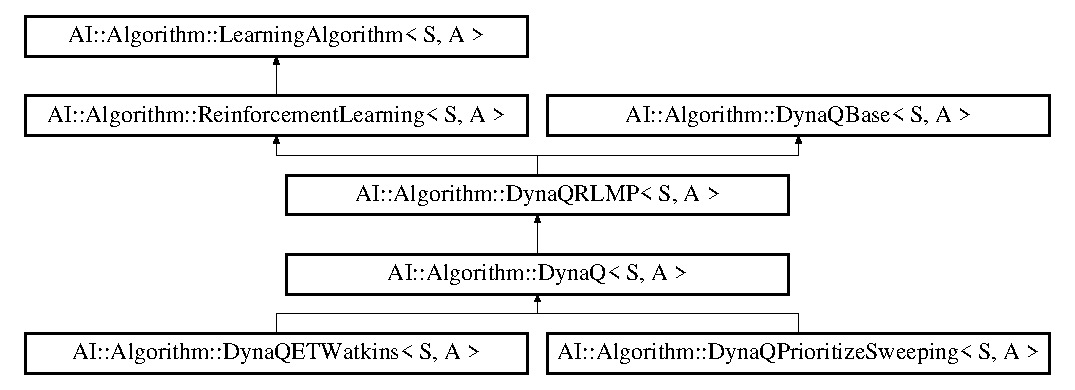
\includegraphics[height=4.794520cm]{classAI_1_1Algorithm_1_1DynaQRLMP}
\end{center}
\end{figure}
\subsection*{Public Member Functions}
\begin{DoxyCompactItemize}
\item 
\hypertarget{classAI_1_1Algorithm_1_1DynaQRLMP_a83035880e274230c3c50bedeed937550}{{\bfseries Dyna\-Q\-R\-L\-M\-P} (A\-I\-::\-F\-L\-O\-A\-T step\-Size, A\-I\-::\-F\-L\-O\-A\-T discount\-Rate, \hyperlink{classAI_1_1Algorithm_1_1Policy}{Policy}$<$ S, A $>$ \&policy, A\-I\-::\-U\-I\-N\-T simulation\-Iteration\-Count, A\-I\-::\-F\-L\-O\-A\-T state\-Transition\-Greediness, A\-I\-::\-F\-L\-O\-A\-T state\-Transition\-Step\-Size)}\label{classAI_1_1Algorithm_1_1DynaQRLMP_a83035880e274230c3c50bedeed937550}

\item 
\hypertarget{classAI_1_1Algorithm_1_1DynaQRLMP_a7b3b5f3706744290b12c19f786e5e4e4}{virtual void {\bfseries back\-Up\-State\-Action\-Pair} (const \hyperlink{classAI_1_1StateAction}{State\-Action}$<$ S, A $>$ \&current\-State\-Action, const A\-I\-::\-F\-L\-O\-A\-T reward, const \hyperlink{classAI_1_1StateAction}{State\-Action}$<$ S, A $>$ \&next\-State\-Action\-Pair)}\label{classAI_1_1Algorithm_1_1DynaQRLMP_a7b3b5f3706744290b12c19f786e5e4e4}

\item 
\hypertarget{classAI_1_1Algorithm_1_1DynaQRLMP_a57a8d01392c4a3699853f3aa623d9ebf}{virtual A {\bfseries arg\-Max} (const S \&state, const set$<$ A $>$ \&action\-Set) const }\label{classAI_1_1Algorithm_1_1DynaQRLMP_a57a8d01392c4a3699853f3aa623d9ebf}

\end{DoxyCompactItemize}
\subsection*{Additional Inherited Members}


The documentation for this class was generated from the following file\-:\begin{DoxyCompactItemize}
\item 
Algorithms/\-Reinforcement\-Learning/Dyna\-Q\-R\-L\-M\-P.\-h\end{DoxyCompactItemize}

\hypertarget{classAI_1_1Algorithm_1_1EligibilityTraces}{\section{A\-I\-:\-:Algorithm\-:\-:Eligibility\-Traces$<$ S, A $>$ Class Template Reference}
\label{classAI_1_1Algorithm_1_1EligibilityTraces}\index{A\-I\-::\-Algorithm\-::\-Eligibility\-Traces$<$ S, A $>$@{A\-I\-::\-Algorithm\-::\-Eligibility\-Traces$<$ S, A $>$}}
}


{\ttfamily \#include $<$Eligibility\-Traces.\-h$>$}

Inheritance diagram for A\-I\-:\-:Algorithm\-:\-:Eligibility\-Traces$<$ S, A $>$\-:\begin{figure}[H]
\begin{center}
\leavevmode
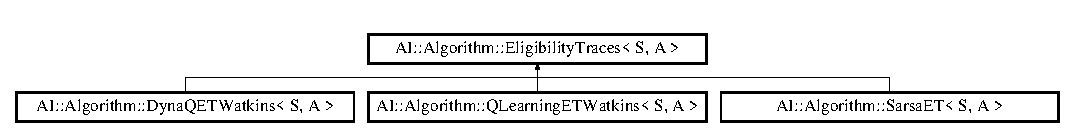
\includegraphics[height=1.408805cm]{classAI_1_1Algorithm_1_1EligibilityTraces}
\end{center}
\end{figure}
\subsection*{Public Member Functions}
\begin{DoxyCompactItemize}
\item 
\hyperlink{classAI_1_1Algorithm_1_1EligibilityTraces_a5ee88e5ac3059733c38a95dba54f677d}{Eligibility\-Traces} (\hyperlink{namespaceAI_a41b74884a20833db653dded3918e05c3}{A\-I\-::\-F\-L\-O\-A\-T} lambda)
\item 
void \hyperlink{classAI_1_1Algorithm_1_1EligibilityTraces_ac52edaa0eeaf4446edb14f7b5415819f}{set\-Lambda} (\hyperlink{namespaceAI_a41b74884a20833db653dded3918e05c3}{A\-I\-::\-F\-L\-O\-A\-T} lambda)
\item 
\hyperlink{namespaceAI_a41b74884a20833db653dded3918e05c3}{A\-I\-::\-F\-L\-O\-A\-T} \hyperlink{classAI_1_1Algorithm_1_1EligibilityTraces_aea9a2c36874a3df328efdf4077ea1c19}{get\-Lambda} () const 
\end{DoxyCompactItemize}
\subsection*{Protected Member Functions}
\begin{DoxyCompactItemize}
\item 
\hypertarget{classAI_1_1Algorithm_1_1EligibilityTraces_a354115a368dc58abcdbc9285ec2537df}{virtual void {\bfseries \-\_\-update\-Eligibility\-Traces} (const \hyperlink{classAI_1_1StateAction}{State\-Action}$<$ S, A $>$ \&current\-State\-Action, const \hyperlink{classAI_1_1StateAction}{State\-Action}$<$ S, A $>$ \&next\-State\-Action, \hyperlink{namespaceAI_a41b74884a20833db653dded3918e05c3}{A\-I\-::\-F\-L\-O\-A\-T} reward, \hyperlink{classAI_1_1StateActionPairContainer}{State\-Action\-Pair\-Container}$<$ S, A $>$ \&state\-Action\-Pair\-Value\-Map, \hyperlink{namespaceAI_a41b74884a20833db653dded3918e05c3}{A\-I\-::\-F\-L\-O\-A\-T} step\-Size, \hyperlink{namespaceAI_a41b74884a20833db653dded3918e05c3}{A\-I\-::\-F\-L\-O\-A\-T} discount\-Rate)}\label{classAI_1_1Algorithm_1_1EligibilityTraces_a354115a368dc58abcdbc9285ec2537df}

\end{DoxyCompactItemize}
\subsection*{Protected Attributes}
\begin{DoxyCompactItemize}
\item 
\hypertarget{classAI_1_1Algorithm_1_1EligibilityTraces_a5c7e8c5c912cd0402cd4d60fb7c34da3}{\hyperlink{namespaceAI_a41b74884a20833db653dded3918e05c3}{A\-I\-::\-F\-L\-O\-A\-T} {\bfseries \-\_\-lambda}}\label{classAI_1_1Algorithm_1_1EligibilityTraces_a5c7e8c5c912cd0402cd4d60fb7c34da3}

\item 
\hypertarget{classAI_1_1Algorithm_1_1EligibilityTraces_aa4a94928533e63cb6b263f7abfde4e53}{map$<$ \hyperlink{classAI_1_1StateAction}{State\-Action}$<$ S, A $>$\\*
, \hyperlink{namespaceAI_a41b74884a20833db653dded3918e05c3}{A\-I\-::\-F\-L\-O\-A\-T} $>$ {\bfseries \-\_\-eligibility\-Traces}}\label{classAI_1_1Algorithm_1_1EligibilityTraces_aa4a94928533e63cb6b263f7abfde4e53}

\end{DoxyCompactItemize}


\subsection{Detailed Description}
\subsubsection*{template$<$class S, class A$>$class A\-I\-::\-Algorithm\-::\-Eligibility\-Traces$<$ S, A $>$}

\hyperlink{classAI_1_1Algorithm_1_1EligibilityTraces}{Eligibility\-Traces} As opposed to ordinary Temporal Difference or whats called in the literature as T\-D(0), eligibility traces T\-D(lambda) bridges the gap between T\-D(0) and Monte Carlo methods. A huge lambda means basically back up ranging from terminal state to initial state. Small lambda converges to T\-D(0).

Note that there is a performance penalty as result of having to iterate all of state space.

T\-O\-D\-O\-: Make another parent class for all other eligibility trace algorithm that contains a merge of R\-L and Eligibility traces. This way, we can syc some shit.

T\-O\-D\-O\-: Connect the reset() to reset\-Eligibility\-Traces() function that have yet to be made. 

\subsection{Constructor \& Destructor Documentation}
\hypertarget{classAI_1_1Algorithm_1_1EligibilityTraces_a5ee88e5ac3059733c38a95dba54f677d}{\index{A\-I\-::\-Algorithm\-::\-Eligibility\-Traces@{A\-I\-::\-Algorithm\-::\-Eligibility\-Traces}!Eligibility\-Traces@{Eligibility\-Traces}}
\index{Eligibility\-Traces@{Eligibility\-Traces}!AI::Algorithm::EligibilityTraces@{A\-I\-::\-Algorithm\-::\-Eligibility\-Traces}}
\subsubsection[{Eligibility\-Traces}]{\setlength{\rightskip}{0pt plus 5cm}template$<$class S , class A $>$ {\bf A\-I\-::\-Algorithm\-::\-Eligibility\-Traces}$<$ S, A $>$\-::{\bf Eligibility\-Traces} (
\begin{DoxyParamCaption}
\item[{{\bf A\-I\-::\-F\-L\-O\-A\-T}}]{lambda}
\end{DoxyParamCaption}
)}}\label{classAI_1_1Algorithm_1_1EligibilityTraces_a5ee88e5ac3059733c38a95dba54f677d}

\begin{DoxyParams}{Parameters}
{\em lambda} & A huge lambda means basically back up ranging from terminal state to initial state. Small lambda converges to T\-D(0). \\
\hline
\end{DoxyParams}


\subsection{Member Function Documentation}
\hypertarget{classAI_1_1Algorithm_1_1EligibilityTraces_aea9a2c36874a3df328efdf4077ea1c19}{\index{A\-I\-::\-Algorithm\-::\-Eligibility\-Traces@{A\-I\-::\-Algorithm\-::\-Eligibility\-Traces}!get\-Lambda@{get\-Lambda}}
\index{get\-Lambda@{get\-Lambda}!AI::Algorithm::EligibilityTraces@{A\-I\-::\-Algorithm\-::\-Eligibility\-Traces}}
\subsubsection[{get\-Lambda}]{\setlength{\rightskip}{0pt plus 5cm}template$<$class S , class A $>$ {\bf A\-I\-::\-F\-L\-O\-A\-T} {\bf A\-I\-::\-Algorithm\-::\-Eligibility\-Traces}$<$ S, A $>$\-::get\-Lambda (
\begin{DoxyParamCaption}
{}
\end{DoxyParamCaption}
) const}}\label{classAI_1_1Algorithm_1_1EligibilityTraces_aea9a2c36874a3df328efdf4077ea1c19}
\begin{DoxyReturn}{Returns}
current lambda. 
\end{DoxyReturn}
\hypertarget{classAI_1_1Algorithm_1_1EligibilityTraces_ac52edaa0eeaf4446edb14f7b5415819f}{\index{A\-I\-::\-Algorithm\-::\-Eligibility\-Traces@{A\-I\-::\-Algorithm\-::\-Eligibility\-Traces}!set\-Lambda@{set\-Lambda}}
\index{set\-Lambda@{set\-Lambda}!AI::Algorithm::EligibilityTraces@{A\-I\-::\-Algorithm\-::\-Eligibility\-Traces}}
\subsubsection[{set\-Lambda}]{\setlength{\rightskip}{0pt plus 5cm}template$<$class S , class A $>$ void {\bf A\-I\-::\-Algorithm\-::\-Eligibility\-Traces}$<$ S, A $>$\-::set\-Lambda (
\begin{DoxyParamCaption}
\item[{{\bf A\-I\-::\-F\-L\-O\-A\-T}}]{lambda}
\end{DoxyParamCaption}
)}}\label{classAI_1_1Algorithm_1_1EligibilityTraces_ac52edaa0eeaf4446edb14f7b5415819f}

\begin{DoxyParams}{Parameters}
{\em lambda} & \\
\hline
\end{DoxyParams}


The documentation for this class was generated from the following file\-:\begin{DoxyCompactItemize}
\item 
Algorithms/\-Reinforcement\-Learning/Eligibility\-Traces.\-h\end{DoxyCompactItemize}

\hypertarget{classAI_1_1Algorithm_1_1Policy_1_1EpsilonGreedy}{\section{A\-I\-:\-:Algorithm\-:\-:Policy\-:\-:Epsilon\-Greedy$<$ S, A $>$ Class Template Reference}
\label{classAI_1_1Algorithm_1_1Policy_1_1EpsilonGreedy}\index{A\-I\-::\-Algorithm\-::\-Policy\-::\-Epsilon\-Greedy$<$ S, A $>$@{A\-I\-::\-Algorithm\-::\-Policy\-::\-Epsilon\-Greedy$<$ S, A $>$}}
}


Selects greedy action with probability {\itshape greediness}  




{\ttfamily \#include $<$Epsilon\-Greedy.\-h$>$}

Inheritance diagram for A\-I\-:\-:Algorithm\-:\-:Policy\-:\-:Epsilon\-Greedy$<$ S, A $>$\-:\begin{figure}[H]
\begin{center}
\leavevmode
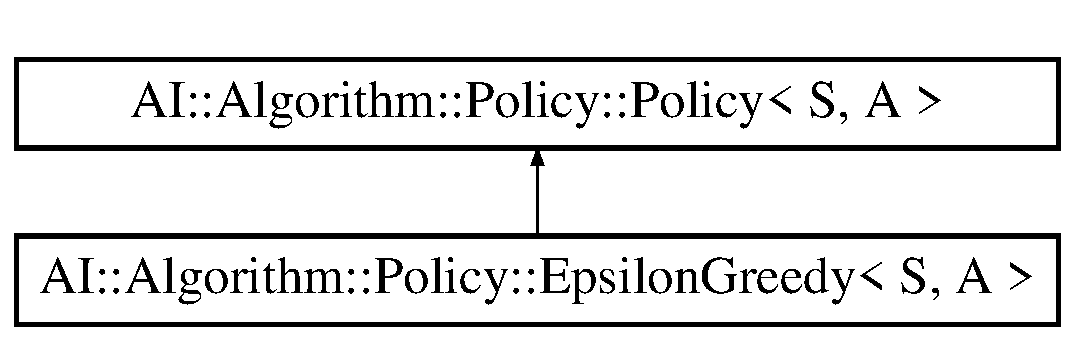
\includegraphics[height=2.000000cm]{classAI_1_1Algorithm_1_1Policy_1_1EpsilonGreedy}
\end{center}
\end{figure}
\subsection*{Public Member Functions}
\begin{DoxyCompactItemize}
\item 
\hyperlink{classAI_1_1Algorithm_1_1Policy_1_1EpsilonGreedy_ab891821ceb3fee0f098ceefad9f5a076}{Epsilon\-Greedy} (A\-I\-::\-F\-L\-O\-A\-T greediness)
\item 
const A \& \hyperlink{classAI_1_1Algorithm_1_1Policy_1_1EpsilonGreedy_a1a7489821592b81576e5bc8674fc43c3}{arg\-Max} (const map$<$ A, A\-I\-::\-F\-L\-O\-A\-T $>$ \&action\-Values, const set$<$ A $>$ \&action\-Set) const 
\item 
virtual const A \& \hyperlink{classAI_1_1Algorithm_1_1Policy_1_1EpsilonGreedy_a00a2dde7f4df14fd046e034694184f65}{get\-Action} (const map$<$ A, A\-I\-::\-F\-L\-O\-A\-T $>$ \&action\-Values, const set$<$ A $>$ \&action\-Set)
\item 
void \hyperlink{classAI_1_1Algorithm_1_1Policy_1_1EpsilonGreedy_a2de58f47fa1663ff4718038f2b268295}{set\-Greediness} (A\-I\-::\-F\-L\-O\-A\-T greediness)
\item 
A\-I\-::\-F\-L\-O\-A\-T \hyperlink{classAI_1_1Algorithm_1_1Policy_1_1EpsilonGreedy_aac2b63fbb3cf29eb8ea11f21d8d6185d}{get\-Greediness} () const 
\end{DoxyCompactItemize}
\subsection*{Protected Attributes}
\begin{DoxyCompactItemize}
\item 
\hypertarget{classAI_1_1Algorithm_1_1Policy_1_1EpsilonGreedy_a54f479df739292986b34a7c79c1d9dee}{random\-\_\-device {\bfseries \-\_\-random\-Device}}\label{classAI_1_1Algorithm_1_1Policy_1_1EpsilonGreedy_a54f479df739292986b34a7c79c1d9dee}

\item 
\hypertarget{classAI_1_1Algorithm_1_1Policy_1_1EpsilonGreedy_af9535e90c13a9a47074721d72a765339}{uniform\-\_\-real\-\_\-distribution\\*
$<$ A\-I\-::\-F\-L\-O\-A\-T $>$ {\bfseries \-\_\-distribution}}\label{classAI_1_1Algorithm_1_1Policy_1_1EpsilonGreedy_af9535e90c13a9a47074721d72a765339}

\item 
\hypertarget{classAI_1_1Algorithm_1_1Policy_1_1EpsilonGreedy_a2726a82fb23e6960c24402a756fef356}{A\-I\-::\-F\-L\-O\-A\-T \hyperlink{classAI_1_1Algorithm_1_1Policy_1_1EpsilonGreedy_a2726a82fb23e6960c24402a756fef356}{\-\_\-greediness}}\label{classAI_1_1Algorithm_1_1Policy_1_1EpsilonGreedy_a2726a82fb23e6960c24402a756fef356}

\begin{DoxyCompactList}\small\item\em Probability of selecting a greedy action. \end{DoxyCompactList}\end{DoxyCompactItemize}


\subsection{Detailed Description}
\subsubsection*{template$<$class S, class A$>$class A\-I\-::\-Algorithm\-::\-Policy\-::\-Epsilon\-Greedy$<$ S, A $>$}

Selects greedy action with probability {\itshape greediness} 

Let $ 0 \leq greediness < 1 $, which is the probability of selecting optimal action. During the selection of non-\/optimal, they are selected in equiprobable manner.


\begin{DoxyTemplParams}{Template Parameters}
{\em S} & State data type. \\
\hline
{\em A} & Action data type. \\
\hline
\end{DoxyTemplParams}


\subsection{Constructor \& Destructor Documentation}
\hypertarget{classAI_1_1Algorithm_1_1Policy_1_1EpsilonGreedy_ab891821ceb3fee0f098ceefad9f5a076}{\index{A\-I\-::\-Algorithm\-::\-Policy\-::\-Epsilon\-Greedy@{A\-I\-::\-Algorithm\-::\-Policy\-::\-Epsilon\-Greedy}!Epsilon\-Greedy@{Epsilon\-Greedy}}
\index{Epsilon\-Greedy@{Epsilon\-Greedy}!AI::Algorithm::Policy::EpsilonGreedy@{A\-I\-::\-Algorithm\-::\-Policy\-::\-Epsilon\-Greedy}}
\subsubsection[{Epsilon\-Greedy}]{\setlength{\rightskip}{0pt plus 5cm}template$<$class S , class A $>$ {\bf A\-I\-::\-Algorithm\-::\-Policy\-::\-Epsilon\-Greedy}$<$ S, A $>$\-::{\bf Epsilon\-Greedy} (
\begin{DoxyParamCaption}
\item[{A\-I\-::\-F\-L\-O\-A\-T}]{greediness}
\end{DoxyParamCaption}
)}}\label{classAI_1_1Algorithm_1_1Policy_1_1EpsilonGreedy_ab891821ceb3fee0f098ceefad9f5a076}

\begin{DoxyParams}{Parameters}
{\em greediness} & probability of selecting greedy action. \\
\hline
\end{DoxyParams}


\subsection{Member Function Documentation}
\hypertarget{classAI_1_1Algorithm_1_1Policy_1_1EpsilonGreedy_a1a7489821592b81576e5bc8674fc43c3}{\index{A\-I\-::\-Algorithm\-::\-Policy\-::\-Epsilon\-Greedy@{A\-I\-::\-Algorithm\-::\-Policy\-::\-Epsilon\-Greedy}!arg\-Max@{arg\-Max}}
\index{arg\-Max@{arg\-Max}!AI::Algorithm::Policy::EpsilonGreedy@{A\-I\-::\-Algorithm\-::\-Policy\-::\-Epsilon\-Greedy}}
\subsubsection[{arg\-Max}]{\setlength{\rightskip}{0pt plus 5cm}template$<$class S , class A$>$ const A \& {\bf A\-I\-::\-Algorithm\-::\-Policy\-::\-Epsilon\-Greedy}$<$ S, A $>$\-::arg\-Max (
\begin{DoxyParamCaption}
\item[{const map$<$ A, A\-I\-::\-F\-L\-O\-A\-T $>$ \&}]{action\-Values, }
\item[{const set$<$ A $>$ \&}]{action\-Set}
\end{DoxyParamCaption}
) const}}\label{classAI_1_1Algorithm_1_1Policy_1_1EpsilonGreedy_a1a7489821592b81576e5bc8674fc43c3}
Returns the action that will \char`\"{}likely\char`\"{} gives the highest reward from the current state.


\begin{DoxyParams}{Parameters}
{\em state} & the state to apply the arg\-Max to. \\
\hline
{\em state\-Action} & map of \hyperlink{classAI_1_1StateAction}{State\-Action} to value. \\
\hline
{\em action\-Set} & a set of possible actions. \\
\hline
\end{DoxyParams}
\begin{DoxyReturn}{Returns}
the action that will \char`\"{}likely\char`\"{} gives the highest reward. 
\end{DoxyReturn}
\hypertarget{classAI_1_1Algorithm_1_1Policy_1_1EpsilonGreedy_a00a2dde7f4df14fd046e034694184f65}{\index{A\-I\-::\-Algorithm\-::\-Policy\-::\-Epsilon\-Greedy@{A\-I\-::\-Algorithm\-::\-Policy\-::\-Epsilon\-Greedy}!get\-Action@{get\-Action}}
\index{get\-Action@{get\-Action}!AI::Algorithm::Policy::EpsilonGreedy@{A\-I\-::\-Algorithm\-::\-Policy\-::\-Epsilon\-Greedy}}
\subsubsection[{get\-Action}]{\setlength{\rightskip}{0pt plus 5cm}template$<$class S , class A$>$ const A \& {\bf A\-I\-::\-Algorithm\-::\-Policy\-::\-Epsilon\-Greedy}$<$ S, A $>$\-::get\-Action (
\begin{DoxyParamCaption}
\item[{const map$<$ A, A\-I\-::\-F\-L\-O\-A\-T $>$ \&}]{action\-Values, }
\item[{const set$<$ A $>$ \&}]{action\-Set}
\end{DoxyParamCaption}
)\hspace{0.3cm}{\ttfamily [virtual]}}}\label{classAI_1_1Algorithm_1_1Policy_1_1EpsilonGreedy_a00a2dde7f4df14fd046e034694184f65}
Returns {\bfseries action} given a mapping of actions and their value and a set of actions.


\begin{DoxyParams}{Parameters}
{\em action\-Values} & a mapping of actions to their corresponding value. \\
\hline
{\em action\-Set} & set of actions. \\
\hline
\end{DoxyParams}
\begin{DoxyReturn}{Returns}
{\bfseries action} given a mapping of actions and their value and a set of actions. 
\end{DoxyReturn}


Implements \hyperlink{classAI_1_1Algorithm_1_1Policy_1_1Policy_a1bd1f511d0f5dce4f4b080232845852c}{A\-I\-::\-Algorithm\-::\-Policy\-::\-Policy$<$ S, A $>$}.

\hypertarget{classAI_1_1Algorithm_1_1Policy_1_1EpsilonGreedy_aac2b63fbb3cf29eb8ea11f21d8d6185d}{\index{A\-I\-::\-Algorithm\-::\-Policy\-::\-Epsilon\-Greedy@{A\-I\-::\-Algorithm\-::\-Policy\-::\-Epsilon\-Greedy}!get\-Greediness@{get\-Greediness}}
\index{get\-Greediness@{get\-Greediness}!AI::Algorithm::Policy::EpsilonGreedy@{A\-I\-::\-Algorithm\-::\-Policy\-::\-Epsilon\-Greedy}}
\subsubsection[{get\-Greediness}]{\setlength{\rightskip}{0pt plus 5cm}template$<$class S , class A $>$ A\-I\-::\-F\-L\-O\-A\-T {\bf A\-I\-::\-Algorithm\-::\-Policy\-::\-Epsilon\-Greedy}$<$ S, A $>$\-::get\-Greediness (
\begin{DoxyParamCaption}
{}
\end{DoxyParamCaption}
) const}}\label{classAI_1_1Algorithm_1_1Policy_1_1EpsilonGreedy_aac2b63fbb3cf29eb8ea11f21d8d6185d}
\begin{DoxyReturn}{Returns}
current greediness. 
\end{DoxyReturn}
\hypertarget{classAI_1_1Algorithm_1_1Policy_1_1EpsilonGreedy_a2de58f47fa1663ff4718038f2b268295}{\index{A\-I\-::\-Algorithm\-::\-Policy\-::\-Epsilon\-Greedy@{A\-I\-::\-Algorithm\-::\-Policy\-::\-Epsilon\-Greedy}!set\-Greediness@{set\-Greediness}}
\index{set\-Greediness@{set\-Greediness}!AI::Algorithm::Policy::EpsilonGreedy@{A\-I\-::\-Algorithm\-::\-Policy\-::\-Epsilon\-Greedy}}
\subsubsection[{set\-Greediness}]{\setlength{\rightskip}{0pt plus 5cm}template$<$class S , class A $>$ void {\bf A\-I\-::\-Algorithm\-::\-Policy\-::\-Epsilon\-Greedy}$<$ S, A $>$\-::set\-Greediness (
\begin{DoxyParamCaption}
\item[{A\-I\-::\-F\-L\-O\-A\-T}]{greediness}
\end{DoxyParamCaption}
)}}\label{classAI_1_1Algorithm_1_1Policy_1_1EpsilonGreedy_a2de58f47fa1663ff4718038f2b268295}

\begin{DoxyParams}{Parameters}
{\em greediness} & \\
\hline
\end{DoxyParams}


The documentation for this class was generated from the following file\-:\begin{DoxyCompactItemize}
\item 
Algorithms/\-Policy/Epsilon\-Greedy.\-h\end{DoxyCompactItemize}

\hypertarget{classAI_1_1Algorithm_1_1GradientDescent}{\section{A\-I\-:\-:Algorithm\-:\-:Gradient\-Descent Class Reference}
\label{classAI_1_1Algorithm_1_1GradientDescent}\index{A\-I\-::\-Algorithm\-::\-Gradient\-Descent@{A\-I\-::\-Algorithm\-::\-Gradient\-Descent}}
}
Inheritance diagram for A\-I\-:\-:Algorithm\-:\-:Gradient\-Descent\-:\begin{figure}[H]
\begin{center}
\leavevmode
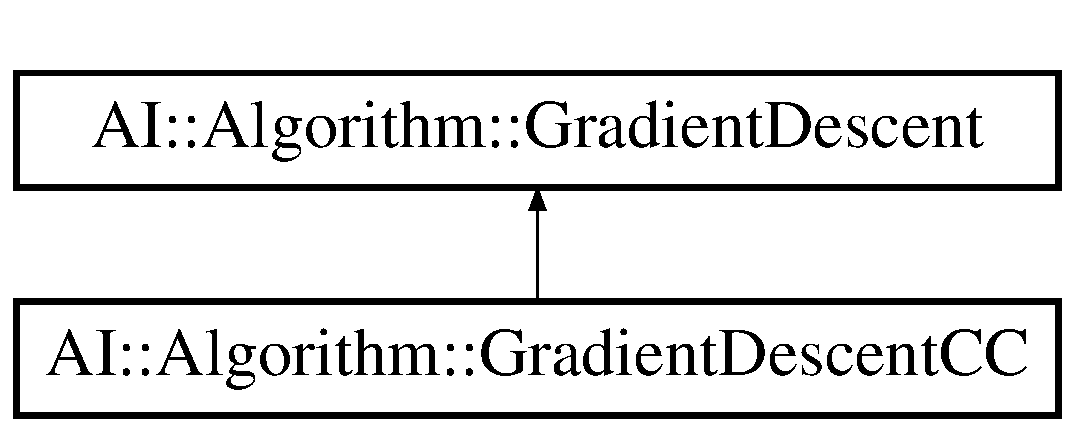
\includegraphics[height=2.000000cm]{classAI_1_1Algorithm_1_1GradientDescent}
\end{center}
\end{figure}
\subsection*{Public Member Functions}
\begin{DoxyCompactItemize}
\item 
\hypertarget{classAI_1_1Algorithm_1_1GradientDescent_a8432f6a139bfac60422558841e6b79ad}{{\bfseries Gradient\-Descent} (\hyperlink{classAI_1_1Algorithm_1_1TileCode}{Tile\-Code} \&tile\-Code, \hyperlink{namespaceAI_a41b74884a20833db653dded3918e05c3}{A\-I\-::\-F\-L\-O\-A\-T} step\-Size, \hyperlink{namespaceAI_a41b74884a20833db653dded3918e05c3}{A\-I\-::\-F\-L\-O\-A\-T} discount\-Rate, \hyperlink{namespaceAI_a41b74884a20833db653dded3918e05c3}{A\-I\-::\-F\-L\-O\-A\-T} lambda)}\label{classAI_1_1Algorithm_1_1GradientDescent_a8432f6a139bfac60422558841e6b79ad}

\item 
size\-\_\-t \hyperlink{classAI_1_1Algorithm_1_1GradientDescent_a04a6c7f4c2e0046dd70b2cfd98322971}{get\-Size} () const 
\item 
\hyperlink{namespaceAI_a41b74884a20833db653dded3918e05c3}{F\-L\-O\-A\-T} \hyperlink{classAI_1_1Algorithm_1_1GradientDescent_a8dcc60ebf28babbe120fe7b20334380f}{get\-Value\-From\-Parameters} (const vector$<$ \hyperlink{namespaceAI_a41b74884a20833db653dded3918e05c3}{F\-L\-O\-A\-T} $>$ \&parameters) const 
\item 
\hyperlink{namespaceAI_a41b74884a20833db653dded3918e05c3}{F\-L\-O\-A\-T} \hyperlink{classAI_1_1Algorithm_1_1GradientDescent_a19111aa6a83836a2e12e623e4004c4d3}{get\-Value\-From\-Feature\-Vector} (const \hyperlink{namespaceAI_a23a39e1b301a5c1345fa508796940631}{F\-E\-A\-T\-U\-R\-E\-\_\-\-V\-E\-C\-T\-O\-R} \&fv) const 
\item 
\hypertarget{classAI_1_1Algorithm_1_1GradientDescent_a6a625b771afbda36509c2b38843825bf}{void {\bfseries get\-Feature\-Vector} (const vector$<$ \hyperlink{namespaceAI_a41b74884a20833db653dded3918e05c3}{F\-L\-O\-A\-T} $>$ \&parameters, \hyperlink{namespaceAI_a23a39e1b301a5c1345fa508796940631}{F\-E\-A\-T\-U\-R\-E\-\_\-\-V\-E\-C\-T\-O\-R} \&fv) const }\label{classAI_1_1Algorithm_1_1GradientDescent_a6a625b771afbda36509c2b38843825bf}

\item 
\hypertarget{classAI_1_1Algorithm_1_1GradientDescent_a68b6d1772a25ce2d6d98cfd3ab697b02}{void {\bfseries increment\-Eligibility\-Traces} (const \hyperlink{namespaceAI_a23a39e1b301a5c1345fa508796940631}{F\-E\-A\-T\-U\-R\-E\-\_\-\-V\-E\-C\-T\-O\-R} \&fv)}\label{classAI_1_1Algorithm_1_1GradientDescent_a68b6d1772a25ce2d6d98cfd3ab697b02}

\item 
\hypertarget{classAI_1_1Algorithm_1_1GradientDescent_ae0038bf21f9576cfa0d24a942f0a6c5a}{void {\bfseries replace\-Eligibility\-Traces} (const \hyperlink{namespaceAI_a23a39e1b301a5c1345fa508796940631}{F\-E\-A\-T\-U\-R\-E\-\_\-\-V\-E\-C\-T\-O\-R} \&fv)}\label{classAI_1_1Algorithm_1_1GradientDescent_ae0038bf21f9576cfa0d24a942f0a6c5a}

\item 
\hypertarget{classAI_1_1Algorithm_1_1GradientDescent_a80faa3771790c726f20f2edff4ad8ff5}{void {\bfseries update\-Weights} (const vector$<$ \hyperlink{namespaceAI_a41b74884a20833db653dded3918e05c3}{F\-L\-O\-A\-T} $>$ \&state\-Vector, const action\-Vector$<$ \hyperlink{namespaceAI_a41b74884a20833db653dded3918e05c3}{F\-L\-O\-A\-T} $>$ \&av, const vector$<$ \hyperlink{namespaceAI_a41b74884a20833db653dded3918e05c3}{F\-L\-O\-A\-T} $>$ \&next\-State, const \hyperlink{namespaceAI_a41b74884a20833db653dded3918e05c3}{F\-L\-O\-A\-T} reward, const set$<$ action\-Vector$<$ \hyperlink{namespaceAI_a41b74884a20833db653dded3918e05c3}{F\-L\-O\-A\-T} $>$ $>$ \&action\-Set)}\label{classAI_1_1Algorithm_1_1GradientDescent_a80faa3771790c726f20f2edff4ad8ff5}

\item 
\hypertarget{classAI_1_1Algorithm_1_1GradientDescent_ab9193530a8d9c61f38707c5a3fc995eb}{void {\bfseries update\-Weights} (const vector$<$ \hyperlink{namespaceAI_a41b74884a20833db653dded3918e05c3}{F\-L\-O\-A\-T} $>$ \&current\-State\-Vector, const action\-Vector$<$ \hyperlink{namespaceAI_a41b74884a20833db653dded3918e05c3}{F\-L\-O\-A\-T} $>$ \&current\-Action\-Vector, const vector$<$ \hyperlink{namespaceAI_a41b74884a20833db653dded3918e05c3}{F\-L\-O\-A\-T} $>$ \&next\-State\-Vector, const vector$<$ \hyperlink{namespaceAI_a41b74884a20833db653dded3918e05c3}{F\-L\-O\-A\-T} $>$ \&next\-Action, const \hyperlink{namespaceAI_a41b74884a20833db653dded3918e05c3}{F\-L\-O\-A\-T} reward)}\label{classAI_1_1Algorithm_1_1GradientDescent_ab9193530a8d9c61f38707c5a3fc995eb}

\item 
\hypertarget{classAI_1_1Algorithm_1_1GradientDescent_a353e283f916955efd47a830425583210}{void {\bfseries update\-Weights} (const vector$<$ \hyperlink{namespaceAI_a41b74884a20833db653dded3918e05c3}{F\-L\-O\-A\-T} $>$ \&current\-State\-Vector, const action\-Vector$<$ \hyperlink{namespaceAI_a41b74884a20833db653dded3918e05c3}{F\-L\-O\-A\-T} $>$ \&current\-Action\-Vector, const vector$<$ \hyperlink{namespaceAI_a41b74884a20833db653dded3918e05c3}{F\-L\-O\-A\-T} $>$ \&next\-State\-Vector, const \hyperlink{namespaceAI_a41b74884a20833db653dded3918e05c3}{F\-L\-O\-A\-T} next\-Action\-Value, const \hyperlink{namespaceAI_a41b74884a20833db653dded3918e05c3}{F\-L\-O\-A\-T} reward)}\label{classAI_1_1Algorithm_1_1GradientDescent_a353e283f916955efd47a830425583210}

\item 
\hypertarget{classAI_1_1Algorithm_1_1GradientDescent_a2ce6e2bbfc5b4d821d02f454c0e3c8c5}{void {\bfseries reset\-Eligibility\-Traces} ()}\label{classAI_1_1Algorithm_1_1GradientDescent_a2ce6e2bbfc5b4d821d02f454c0e3c8c5}

\item 
\hypertarget{classAI_1_1Algorithm_1_1GradientDescent_a7f58c9d3f1c760d5e4d1f9546abb1bec}{void {\bfseries build\-Action\-Values} (const set$<$ action\-Vector$<$ \hyperlink{namespaceAI_a41b74884a20833db653dded3918e05c3}{F\-L\-O\-A\-T} $>$ $>$ \&action\-Set, const vector$<$ \hyperlink{namespaceAI_a41b74884a20833db653dded3918e05c3}{F\-L\-O\-A\-T} $>$ \&param, map$<$ action\-Vector$<$ \hyperlink{namespaceAI_a41b74884a20833db653dded3918e05c3}{F\-L\-O\-A\-T} $>$, \hyperlink{namespaceAI_a41b74884a20833db653dded3918e05c3}{F\-L\-O\-A\-T} $>$ \&action\-Vector\-Value\-Map) const }\label{classAI_1_1Algorithm_1_1GradientDescent_a7f58c9d3f1c760d5e4d1f9546abb1bec}

\item 
\hypertarget{classAI_1_1Algorithm_1_1GradientDescent_a651b2804acf14aaebdf461d39cd970eb}{\hyperlink{namespaceAI_a41b74884a20833db653dded3918e05c3}{F\-L\-O\-A\-T} {\bfseries get\-Max\-Value} (const map$<$ action\-Vector$<$ \hyperlink{namespaceAI_a41b74884a20833db653dded3918e05c3}{F\-L\-O\-A\-T} $>$, \hyperlink{namespaceAI_a41b74884a20833db653dded3918e05c3}{F\-L\-O\-A\-T} $>$ \&action\-Value\-Map) const }\label{classAI_1_1Algorithm_1_1GradientDescent_a651b2804acf14aaebdf461d39cd970eb}

\item 
\hypertarget{classAI_1_1Algorithm_1_1GradientDescent_a5c5ae472417bc016fdd185875614359d}{virtual void {\bfseries decrease\-Eligibility\-Traces} ()}\label{classAI_1_1Algorithm_1_1GradientDescent_a5c5ae472417bc016fdd185875614359d}

\item 
\hypertarget{classAI_1_1Algorithm_1_1GradientDescent_a49b556716f8ca93c088b10f4432a3688}{virtual void {\bfseries back\-Up\-Weights} (\hyperlink{namespaceAI_a41b74884a20833db653dded3918e05c3}{F\-L\-O\-A\-T} td\-Error)}\label{classAI_1_1Algorithm_1_1GradientDescent_a49b556716f8ca93c088b10f4432a3688}

\end{DoxyCompactItemize}
\subsection*{Protected Attributes}
\begin{DoxyCompactItemize}
\item 
\hypertarget{classAI_1_1Algorithm_1_1GradientDescent_a483b6e1985c4a85a59929e137bc0b559}{\hyperlink{classAI_1_1Algorithm_1_1TileCode}{Tile\-Code} \& {\bfseries \-\_\-tile\-Code}}\label{classAI_1_1Algorithm_1_1GradientDescent_a483b6e1985c4a85a59929e137bc0b559}

\item 
\hypertarget{classAI_1_1Algorithm_1_1GradientDescent_ae4eecab645d2f7e8b245d5a25d7b7e63}{vector$<$ \hyperlink{namespaceAI_a41b74884a20833db653dded3918e05c3}{F\-L\-O\-A\-T} $>$ {\bfseries \-\_\-w}}\label{classAI_1_1Algorithm_1_1GradientDescent_ae4eecab645d2f7e8b245d5a25d7b7e63}

\item 
\hypertarget{classAI_1_1Algorithm_1_1GradientDescent_ac759083fba7ad9ef41a7b27d1d946eaf}{vector$<$ \hyperlink{namespaceAI_a41b74884a20833db653dded3918e05c3}{A\-I\-::\-F\-L\-O\-A\-T} $>$ {\bfseries \-\_\-e}}\label{classAI_1_1Algorithm_1_1GradientDescent_ac759083fba7ad9ef41a7b27d1d946eaf}

\item 
\hypertarget{classAI_1_1Algorithm_1_1GradientDescent_a6869d80a15d5a841ae4e64ded72a6618}{\hyperlink{namespaceAI_a41b74884a20833db653dded3918e05c3}{A\-I\-::\-F\-L\-O\-A\-T} {\bfseries \-\_\-step\-Size}}\label{classAI_1_1Algorithm_1_1GradientDescent_a6869d80a15d5a841ae4e64ded72a6618}

\item 
\hypertarget{classAI_1_1Algorithm_1_1GradientDescent_a4667068a5810028bef4e4eb0138da297}{\hyperlink{namespaceAI_a41b74884a20833db653dded3918e05c3}{A\-I\-::\-F\-L\-O\-A\-T} {\bfseries \-\_\-discount\-Rate}}\label{classAI_1_1Algorithm_1_1GradientDescent_a4667068a5810028bef4e4eb0138da297}

\item 
\hypertarget{classAI_1_1Algorithm_1_1GradientDescent_a1babda7cbad2a946ffdc2eaec8507fa5}{\hyperlink{namespaceAI_a41b74884a20833db653dded3918e05c3}{A\-I\-::\-F\-L\-O\-A\-T} {\bfseries \-\_\-lambda}}\label{classAI_1_1Algorithm_1_1GradientDescent_a1babda7cbad2a946ffdc2eaec8507fa5}

\end{DoxyCompactItemize}


\subsection{Member Function Documentation}
\hypertarget{classAI_1_1Algorithm_1_1GradientDescent_a04a6c7f4c2e0046dd70b2cfd98322971}{\index{A\-I\-::\-Algorithm\-::\-Gradient\-Descent@{A\-I\-::\-Algorithm\-::\-Gradient\-Descent}!get\-Size@{get\-Size}}
\index{get\-Size@{get\-Size}!AI::Algorithm::GradientDescent@{A\-I\-::\-Algorithm\-::\-Gradient\-Descent}}
\subsubsection[{get\-Size}]{\setlength{\rightskip}{0pt plus 5cm}size\-\_\-t A\-I\-::\-Algorithm\-::\-Gradient\-Descent\-::get\-Size (
\begin{DoxyParamCaption}
{}
\end{DoxyParamCaption}
) const}}\label{classAI_1_1Algorithm_1_1GradientDescent_a04a6c7f4c2e0046dd70b2cfd98322971}
\begin{DoxyReturn}{Returns}
Size of both weight vector and traces vector. 
\end{DoxyReturn}
\hypertarget{classAI_1_1Algorithm_1_1GradientDescent_a19111aa6a83836a2e12e623e4004c4d3}{\index{A\-I\-::\-Algorithm\-::\-Gradient\-Descent@{A\-I\-::\-Algorithm\-::\-Gradient\-Descent}!get\-Value\-From\-Feature\-Vector@{get\-Value\-From\-Feature\-Vector}}
\index{get\-Value\-From\-Feature\-Vector@{get\-Value\-From\-Feature\-Vector}!AI::Algorithm::GradientDescent@{A\-I\-::\-Algorithm\-::\-Gradient\-Descent}}
\subsubsection[{get\-Value\-From\-Feature\-Vector}]{\setlength{\rightskip}{0pt plus 5cm}{\bf F\-L\-O\-A\-T} A\-I\-::\-Algorithm\-::\-Gradient\-Descent\-::get\-Value\-From\-Feature\-Vector (
\begin{DoxyParamCaption}
\item[{const {\bf F\-E\-A\-T\-U\-R\-E\-\_\-\-V\-E\-C\-T\-O\-R} \&}]{fv}
\end{DoxyParamCaption}
) const}}\label{classAI_1_1Algorithm_1_1GradientDescent_a19111aa6a83836a2e12e623e4004c4d3}
Get the value of the parameters in the real space. 
\begin{DoxyParams}{Parameters}
{\em feature\-Vector} & \\
\hline
\end{DoxyParams}
\begin{DoxyReturn}{Returns}
corresponding value. 
\end{DoxyReturn}
\hypertarget{classAI_1_1Algorithm_1_1GradientDescent_a8dcc60ebf28babbe120fe7b20334380f}{\index{A\-I\-::\-Algorithm\-::\-Gradient\-Descent@{A\-I\-::\-Algorithm\-::\-Gradient\-Descent}!get\-Value\-From\-Parameters@{get\-Value\-From\-Parameters}}
\index{get\-Value\-From\-Parameters@{get\-Value\-From\-Parameters}!AI::Algorithm::GradientDescent@{A\-I\-::\-Algorithm\-::\-Gradient\-Descent}}
\subsubsection[{get\-Value\-From\-Parameters}]{\setlength{\rightskip}{0pt plus 5cm}{\bf F\-L\-O\-A\-T} A\-I\-::\-Algorithm\-::\-Gradient\-Descent\-::get\-Value\-From\-Parameters (
\begin{DoxyParamCaption}
\item[{const vector$<$ {\bf F\-L\-O\-A\-T} $>$ \&}]{parameters}
\end{DoxyParamCaption}
) const}}\label{classAI_1_1Algorithm_1_1GradientDescent_a8dcc60ebf28babbe120fe7b20334380f}
Get the value of the parameters in the real space. 
\begin{DoxyParams}{Parameters}
{\em parameters} & \\
\hline
\end{DoxyParams}
\begin{DoxyReturn}{Returns}
corresponding value. 
\end{DoxyReturn}


The documentation for this class was generated from the following file\-:\begin{DoxyCompactItemize}
\item 
Algorithms/\-Supervised\-Learning/Gradient\-Descent.\-h\end{DoxyCompactItemize}

\hypertarget{classAI_1_1Algorithm_1_1GradientDescentCC}{\section{A\-I\-:\-:Algorithm\-:\-:Gradient\-Descent\-C\-C Class Reference}
\label{classAI_1_1Algorithm_1_1GradientDescentCC}\index{A\-I\-::\-Algorithm\-::\-Gradient\-Descent\-C\-C@{A\-I\-::\-Algorithm\-::\-Gradient\-Descent\-C\-C}}
}
Inheritance diagram for A\-I\-:\-:Algorithm\-:\-:Gradient\-Descent\-C\-C\-:\begin{figure}[H]
\begin{center}
\leavevmode
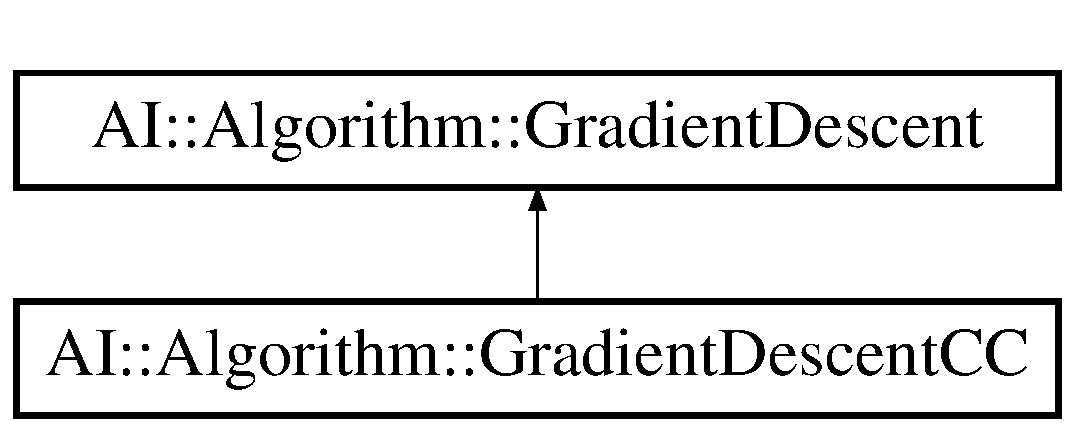
\includegraphics[height=2.000000cm]{classAI_1_1Algorithm_1_1GradientDescentCC}
\end{center}
\end{figure}
\subsection*{Public Member Functions}
\begin{DoxyCompactItemize}
\item 
\hypertarget{classAI_1_1Algorithm_1_1GradientDescentCC_a036943a3f05d8e9146e833d225b13d74}{{\bfseries Gradient\-Descent\-C\-C} (\hyperlink{classAI_1_1Algorithm_1_1TileCode}{Tile\-Code} \&tile\-Code, \hyperlink{namespaceAI_a41b74884a20833db653dded3918e05c3}{A\-I\-::\-F\-L\-O\-A\-T} step\-Size, \hyperlink{namespaceAI_a41b74884a20833db653dded3918e05c3}{A\-I\-::\-F\-L\-O\-A\-T} discount\-Rate, \hyperlink{namespaceAI_a41b74884a20833db653dded3918e05c3}{A\-I\-::\-F\-L\-O\-A\-T} lambda)}\label{classAI_1_1Algorithm_1_1GradientDescentCC_a036943a3f05d8e9146e833d225b13d74}

\item 
\hypertarget{classAI_1_1Algorithm_1_1GradientDescentCC_a5cd9bd033e8556b4961370da3298cfce}{virtual void {\bfseries decrease\-Eligibility\-Traces} ()}\label{classAI_1_1Algorithm_1_1GradientDescentCC_a5cd9bd033e8556b4961370da3298cfce}

\item 
\hypertarget{classAI_1_1Algorithm_1_1GradientDescentCC_a990c4b429edd9583e0e0a56be43faad8}{virtual void {\bfseries back\-Up\-Weights} (\hyperlink{namespaceAI_a41b74884a20833db653dded3918e05c3}{F\-L\-O\-A\-T} td\-Error)}\label{classAI_1_1Algorithm_1_1GradientDescentCC_a990c4b429edd9583e0e0a56be43faad8}

\end{DoxyCompactItemize}
\subsection*{Protected Member Functions}
\begin{DoxyCompactItemize}
\item 
\hypertarget{classAI_1_1Algorithm_1_1GradientDescentCC_a671233415fd282b198c6d0999e63832a}{virtual void {\bfseries \-\_\-decrease\-Eligibility\-Traces\-Worker} (\hyperlink{namespaceAI_ab6e14dc1e659854858a87e511f1439ec}{A\-I\-::\-U\-I\-N\-T} starti, \hyperlink{namespaceAI_ab6e14dc1e659854858a87e511f1439ec}{A\-I\-::\-U\-I\-N\-T} length)}\label{classAI_1_1Algorithm_1_1GradientDescentCC_a671233415fd282b198c6d0999e63832a}

\item 
\hypertarget{classAI_1_1Algorithm_1_1GradientDescentCC_a647a9d1f60731c366695a7c1fac008d4}{virtual void {\bfseries \-\_\-back\-Up\-Weights\-Worker} (\hyperlink{namespaceAI_a41b74884a20833db653dded3918e05c3}{F\-L\-O\-A\-T} td\-Error, \hyperlink{namespaceAI_ab6e14dc1e659854858a87e511f1439ec}{A\-I\-::\-U\-I\-N\-T} starti, \hyperlink{namespaceAI_ab6e14dc1e659854858a87e511f1439ec}{A\-I\-::\-U\-I\-N\-T} length)}\label{classAI_1_1Algorithm_1_1GradientDescentCC_a647a9d1f60731c366695a7c1fac008d4}

\end{DoxyCompactItemize}
\subsection*{Additional Inherited Members}


The documentation for this class was generated from the following file\-:\begin{DoxyCompactItemize}
\item 
Algorithms/\-Supervised\-Learning/Gradient\-Descent\-C\-C.\-h\end{DoxyCompactItemize}

\hypertarget{classAI_1_1Algorithm_1_1Hash_1_1HashInterface}{\section{A\+I\+:\+:Algorithm\+:\+:Hash\+:\+:Hash\+Interface$<$ R\+E\+T $>$ Class Template Reference}
\label{classAI_1_1Algorithm_1_1Hash_1_1HashInterface}\index{A\+I\+::\+Algorithm\+::\+Hash\+::\+Hash\+Interface$<$ R\+E\+T $>$@{A\+I\+::\+Algorithm\+::\+Hash\+::\+Hash\+Interface$<$ R\+E\+T $>$}}
}


Interface for all hash encapsulation.  




{\ttfamily \#include $<$Hash\+Interface.\+h$>$}

\subsection*{Public Member Functions}
\begin{DoxyCompactItemize}
\item 
virtual R\+E\+T \hyperlink{classAI_1_1Algorithm_1_1Hash_1_1HashInterface_ae31d650fd044e3ef372cae18a422e0d9}{hash} (const \hyperlink{namespaceAI_a9d4bcda82fe0f9aac3c4861e24491581}{A\+I\+::\+B\+Y\+T\+E} $\ast$const byte\+Array, size\+\_\+t len)=0
\item 
\hypertarget{classAI_1_1Algorithm_1_1Hash_1_1HashInterface_a960c6305b583d12df2a067191c4a6f58}{virtual R\+E\+T {\bfseries hash} (const vector$<$ \hyperlink{namespaceAI_a9d4bcda82fe0f9aac3c4861e24491581}{A\+I\+::\+B\+Y\+T\+E} $>$ \&byte\+Array)=0}\label{classAI_1_1Algorithm_1_1Hash_1_1HashInterface_a960c6305b583d12df2a067191c4a6f58}

\end{DoxyCompactItemize}


\subsection{Detailed Description}
\subsubsection*{template$<$class R\+E\+T$>$class A\+I\+::\+Algorithm\+::\+Hash\+::\+Hash\+Interface$<$ R\+E\+T $>$}

Interface for all hash encapsulation. 


\begin{DoxyTemplParams}{Template Parameters}
{\em R\+E\+T} & return data type. \\
\hline
\end{DoxyTemplParams}


\subsection{Member Function Documentation}
\hypertarget{classAI_1_1Algorithm_1_1Hash_1_1HashInterface_ae31d650fd044e3ef372cae18a422e0d9}{\index{A\+I\+::\+Algorithm\+::\+Hash\+::\+Hash\+Interface@{A\+I\+::\+Algorithm\+::\+Hash\+::\+Hash\+Interface}!hash@{hash}}
\index{hash@{hash}!A\+I\+::\+Algorithm\+::\+Hash\+::\+Hash\+Interface@{A\+I\+::\+Algorithm\+::\+Hash\+::\+Hash\+Interface}}
\subsubsection[{hash}]{\setlength{\rightskip}{0pt plus 5cm}template$<$class R\+E\+T$>$ virtual R\+E\+T {\bf A\+I\+::\+Algorithm\+::\+Hash\+::\+Hash\+Interface}$<$ R\+E\+T $>$\+::hash (
\begin{DoxyParamCaption}
\item[{const {\bf A\+I\+::\+B\+Y\+T\+E} $\ast$const}]{byte\+Array, }
\item[{size\+\_\+t}]{len}
\end{DoxyParamCaption}
)\hspace{0.3cm}{\ttfamily [pure virtual]}}}\label{classAI_1_1Algorithm_1_1Hash_1_1HashInterface_ae31d650fd044e3ef372cae18a422e0d9}

\begin{DoxyParams}{Parameters}
{\em byte\+Array} & \\
\hline
{\em len} & \\
\hline
\end{DoxyParams}
\begin{DoxyReturn}{Returns}
h(byte\+Array) 
\end{DoxyReturn}


Implemented in \hyperlink{classAI_1_1Algorithm_1_1Hash_1_1Murmur3_ab79d4cbd685e34c88077d58e5cacf7a3}{A\+I\+::\+Algorithm\+::\+Hash\+::\+Murmur3}, \hyperlink{classAI_1_1Algorithm_1_1Hash_1_1UNH_acc52e3c2f323e748882ee5d9d66be698}{A\+I\+::\+Algorithm\+::\+Hash\+::\+U\+N\+H}, and \hyperlink{classAI_1_1Algorithm_1_1Hash_1_1SuperFastHash_a242ccb7975bd45b30a945d9649170629}{A\+I\+::\+Algorithm\+::\+Hash\+::\+Super\+Fast\+Hash}.



The documentation for this class was generated from the following file\+:\begin{DoxyCompactItemize}
\item 
Algorithms/\+Hash/Hash\+Interface.\+h\end{DoxyCompactItemize}

\hypertarget{structAI_1_1Algorithm_1_1Hash_1_1HashMurmur3Out}{\section{A\+I\+:\+:Algorithm\+:\+:Hash\+:\+:Hash\+Murmur3\+Out Struct Reference}
\label{structAI_1_1Algorithm_1_1Hash_1_1HashMurmur3Out}\index{A\+I\+::\+Algorithm\+::\+Hash\+::\+Hash\+Murmur3\+Out@{A\+I\+::\+Algorithm\+::\+Hash\+::\+Hash\+Murmur3\+Out}}
}


Encapsulates the output of the murmur hash. Encapsulates the output of the murmur hash. uint64\+\_\+t hash\+Val\mbox{[}2\mbox{]} is the the array being encapsulated since output of murmur3 hash is 128 bit.  




{\ttfamily \#include $<$Hash\+Murmur3.\+h$>$}

\subsection*{Public Attributes}
\begin{DoxyCompactItemize}
\item 
\hypertarget{structAI_1_1Algorithm_1_1Hash_1_1HashMurmur3Out_a181dd4bb7df2d2c722d4bfa8d88f2c0d}{uint64\+\_\+t {\bfseries hash\+Val} \mbox{[}2\mbox{]}}\label{structAI_1_1Algorithm_1_1Hash_1_1HashMurmur3Out_a181dd4bb7df2d2c722d4bfa8d88f2c0d}

\end{DoxyCompactItemize}


\subsection{Detailed Description}
Encapsulates the output of the murmur hash. Encapsulates the output of the murmur hash. uint64\+\_\+t hash\+Val\mbox{[}2\mbox{]} is the the array being encapsulated since output of murmur3 hash is 128 bit. 

The documentation for this struct was generated from the following file\+:\begin{DoxyCompactItemize}
\item 
Algorithms/\+Hash/Hash\+Murmur3.\+h\end{DoxyCompactItemize}

\hypertarget{classAI_1_1Algorithm_1_1LearningAlgorithm}{\section{A\+I\+:\+:Algorithm\+:\+:Learning\+Algorithm$<$ S, A $>$ Class Template Reference}
\label{classAI_1_1Algorithm_1_1LearningAlgorithm}\index{A\+I\+::\+Algorithm\+::\+Learning\+Algorithm$<$ S, A $>$@{A\+I\+::\+Algorithm\+::\+Learning\+Algorithm$<$ S, A $>$}}
}


Base class for all learning algorithms.  




{\ttfamily \#include $<$Learning\+Algorithm.\+h$>$}

Inheritance diagram for A\+I\+:\+:Algorithm\+:\+:Learning\+Algorithm$<$ S, A $>$\+:\begin{figure}[H]
\begin{center}
\leavevmode
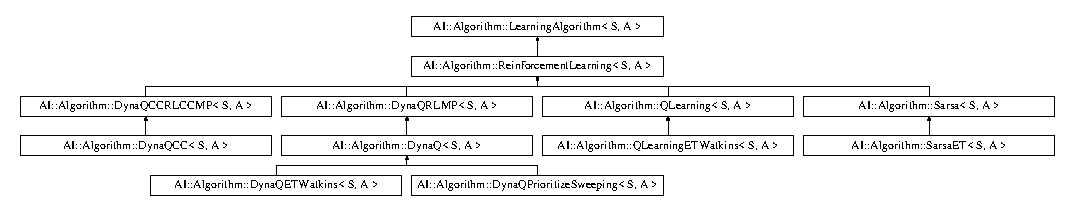
\includegraphics[height=2.397260cm]{classAI_1_1Algorithm_1_1LearningAlgorithm}
\end{center}
\end{figure}
\subsection*{Public Member Functions}
\begin{DoxyCompactItemize}
\item 
\hyperlink{classAI_1_1Algorithm_1_1LearningAlgorithm_a8fe54228193c0d7a28fba7de00441d7f}{Learning\+Algorithm} (\hyperlink{classAI_1_1Algorithm_1_1Policy_1_1Policy}{Policy\+::\+Policy}$<$ S, A $>$ \&control\+Policy)
\item 
virtual void \hyperlink{classAI_1_1Algorithm_1_1LearningAlgorithm_a7d216d791e558e15a73083af6257ed72}{update} (const \hyperlink{classAI_1_1StateAction}{State\+Action}$<$ S, A $>$ \&current\+State\+Action, const S \&next\+State, const \hyperlink{namespaceAI_a41b74884a20833db653dded3918e05c3}{A\+I\+::\+F\+L\+O\+A\+T} reward, const set$<$ A $>$ \&action\+Set)=0
\item 
virtual const A \& \hyperlink{classAI_1_1Algorithm_1_1LearningAlgorithm_afeca4eded9bc0a02312ccbbfd05f8daa}{get\+Action} (const S \&state, const set$<$ A $>$ \&action\+Set)=0
\item 
virtual \hyperlink{namespaceAI_a41b74884a20833db653dded3918e05c3}{A\+I\+::\+F\+L\+O\+A\+T} \hyperlink{classAI_1_1Algorithm_1_1LearningAlgorithm_a1044b2558109e8dd3d3bf5bedb9723b5}{get\+State\+Action\+Value} (const \hyperlink{classAI_1_1StateAction}{State\+Action}$<$ S, A $>$ \&state\+Action)=0
\item 
void \hyperlink{classAI_1_1Algorithm_1_1LearningAlgorithm_a1d26cb76c945a5312ce4ac4fdabc4d31}{se\+Controlt\+Policy} (\hyperlink{classAI_1_1Algorithm_1_1Policy_1_1Policy}{Policy\+::\+Policy}$<$ S, A $>$ \&policy)
\item 
\hyperlink{classAI_1_1Algorithm_1_1Policy_1_1Policy}{Policy\+::\+Policy}$<$ S, A $>$ \& \hyperlink{classAI_1_1Algorithm_1_1LearningAlgorithm_ab123635bc3d527052051c7f4c37a986c}{get\+Control\+Policy} ()
\item 
virtual void \hyperlink{classAI_1_1Algorithm_1_1LearningAlgorithm_aebe650b79f39ffd46ece7adb44ddaf60}{reset} ()
\item 
const \hyperlink{namespaceAI_a41b74884a20833db653dded3918e05c3}{A\+I\+::\+F\+L\+O\+A\+T} \& \hyperlink{classAI_1_1Algorithm_1_1LearningAlgorithm_aafc85fe7b2ad9331ae41593784321641}{get\+Default\+State\+Action\+Value} () const 
\item 
void \hyperlink{classAI_1_1Algorithm_1_1LearningAlgorithm_a1da99bfa2de96f397a4ef07e53ab5697}{set\+Default\+State\+Action\+Value} (const \hyperlink{namespaceAI_a41b74884a20833db653dded3918e05c3}{A\+I\+::\+F\+L\+O\+A\+T} \&default\+State\+Action\+Value)
\item 
void \hyperlink{classAI_1_1Algorithm_1_1LearningAlgorithm_a826f61675ac11b699c4328c44cccdae5}{set\+Learning\+Policy} (\hyperlink{classAI_1_1Algorithm_1_1Policy_1_1Policy}{Policy\+::\+Policy}$<$ S, A $>$ \&policy)
\item 
const \hyperlink{classAI_1_1Algorithm_1_1Policy_1_1Policy}{Policy\+::\+Policy}$<$ S, A $>$ \& \hyperlink{classAI_1_1Algorithm_1_1LearningAlgorithm_aac506aa1838ba12e2069c098d6faec16}{get\+Learning\+Policy} () const 
\end{DoxyCompactItemize}
\subsection*{Protected Member Functions}
\begin{DoxyCompactItemize}
\item 
const A \& \hyperlink{classAI_1_1Algorithm_1_1LearningAlgorithm_ad5b5f6baa9c03f68427008abeeb35535}{\+\_\+get\+Learning\+Policy\+Action} (const map$<$ A, \hyperlink{namespaceAI_a41b74884a20833db653dded3918e05c3}{A\+I\+::\+F\+L\+O\+A\+T} $>$ \&action\+Value\+Map, const set$<$ A $>$ \&action\+Set)
\end{DoxyCompactItemize}
\subsection*{Protected Attributes}
\begin{DoxyCompactItemize}
\item 
\hypertarget{classAI_1_1Algorithm_1_1LearningAlgorithm_ae3b8ccdc51ad2a8c1cc2ef9009258466}{\hyperlink{namespaceAI_a41b74884a20833db653dded3918e05c3}{A\+I\+::\+F\+L\+O\+A\+T} \hyperlink{classAI_1_1Algorithm_1_1LearningAlgorithm_ae3b8ccdc51ad2a8c1cc2ef9009258466}{\+\_\+default\+State\+Action\+Value}}\label{classAI_1_1Algorithm_1_1LearningAlgorithm_ae3b8ccdc51ad2a8c1cc2ef9009258466}

\begin{DoxyCompactList}\small\item\em Place holder for default state action value. \end{DoxyCompactList}\item 
\hypertarget{classAI_1_1Algorithm_1_1LearningAlgorithm_ad74dbed6a7be0c699d42642b9968bf86}{\hyperlink{classAI_1_1Algorithm_1_1Policy_1_1Policy}{Policy\+::\+Policy}$<$ S, A $>$ \& \hyperlink{classAI_1_1Algorithm_1_1LearningAlgorithm_ad74dbed6a7be0c699d42642b9968bf86}{\+\_\+control\+Policy}}\label{classAI_1_1Algorithm_1_1LearningAlgorithm_ad74dbed6a7be0c699d42642b9968bf86}

\begin{DoxyCompactList}\small\item\em Policy for action selection online. \end{DoxyCompactList}\item 
\hypertarget{classAI_1_1Algorithm_1_1LearningAlgorithm_a603f2a2905636a150c0fb9946085837a}{\hyperlink{classAI_1_1Algorithm_1_1Policy_1_1Policy}{Policy\+::\+Policy}$<$ S, A $>$ \& \hyperlink{classAI_1_1Algorithm_1_1LearningAlgorithm_a603f2a2905636a150c0fb9946085837a}{\+\_\+learning\+Policy}}\label{classAI_1_1Algorithm_1_1LearningAlgorithm_a603f2a2905636a150c0fb9946085837a}

\begin{DoxyCompactList}\small\item\em Policy for action selection offline. \end{DoxyCompactList}\end{DoxyCompactItemize}
\subsection*{Static Protected Attributes}
\begin{DoxyCompactItemize}
\item 
\hypertarget{classAI_1_1Algorithm_1_1LearningAlgorithm_ad9b3db3c2443e1a44803ec6d34887485}{static \hyperlink{classAI_1_1Algorithm_1_1Policy_1_1EpsilonGreedy}{Policy\+::\+Epsilon\+Greedy}\\*
$<$ S, A $>$ \hyperlink{classAI_1_1Algorithm_1_1LearningAlgorithm_ad9b3db3c2443e1a44803ec6d34887485}{\+\_\+default\+Learning\+Policy}}\label{classAI_1_1Algorithm_1_1LearningAlgorithm_ad9b3db3c2443e1a44803ec6d34887485}

\begin{DoxyCompactList}\small\item\em Default offline policy. \end{DoxyCompactList}\end{DoxyCompactItemize}


\subsection{Detailed Description}
\subsubsection*{template$<$class S, class A$>$class A\+I\+::\+Algorithm\+::\+Learning\+Algorithm$<$ S, A $>$}

Base class for all learning algorithms. 

All learning algorithm, reinforcement, supervised, unsupervised inherit from this class. 
\begin{DoxyTemplParams}{Template Parameters}
{\em S} & State Data type. \\
\hline
{\em A} & Action Data type. \\
\hline
\end{DoxyTemplParams}


\subsection{Constructor \& Destructor Documentation}
\hypertarget{classAI_1_1Algorithm_1_1LearningAlgorithm_a8fe54228193c0d7a28fba7de00441d7f}{\index{A\+I\+::\+Algorithm\+::\+Learning\+Algorithm@{A\+I\+::\+Algorithm\+::\+Learning\+Algorithm}!Learning\+Algorithm@{Learning\+Algorithm}}
\index{Learning\+Algorithm@{Learning\+Algorithm}!A\+I\+::\+Algorithm\+::\+Learning\+Algorithm@{A\+I\+::\+Algorithm\+::\+Learning\+Algorithm}}
\subsubsection[{Learning\+Algorithm}]{\setlength{\rightskip}{0pt plus 5cm}template$<$class S, class A$>$ {\bf A\+I\+::\+Algorithm\+::\+Learning\+Algorithm}$<$ S, A $>$\+::{\bf Learning\+Algorithm} (
\begin{DoxyParamCaption}
\item[{{\bf Policy\+::\+Policy}$<$ S, A $>$ \&}]{control\+Policy}
\end{DoxyParamCaption}
)}}\label{classAI_1_1Algorithm_1_1LearningAlgorithm_a8fe54228193c0d7a28fba7de00441d7f}

\begin{DoxyParams}{Parameters}
{\em control\+Policy} & policy for action selection online. \\
\hline
\end{DoxyParams}


\subsection{Member Function Documentation}
\hypertarget{classAI_1_1Algorithm_1_1LearningAlgorithm_ad5b5f6baa9c03f68427008abeeb35535}{\index{A\+I\+::\+Algorithm\+::\+Learning\+Algorithm@{A\+I\+::\+Algorithm\+::\+Learning\+Algorithm}!\+\_\+get\+Learning\+Policy\+Action@{\+\_\+get\+Learning\+Policy\+Action}}
\index{\+\_\+get\+Learning\+Policy\+Action@{\+\_\+get\+Learning\+Policy\+Action}!A\+I\+::\+Algorithm\+::\+Learning\+Algorithm@{A\+I\+::\+Algorithm\+::\+Learning\+Algorithm}}
\subsubsection[{\+\_\+get\+Learning\+Policy\+Action}]{\setlength{\rightskip}{0pt plus 5cm}template$<$class S , class A$>$ const A \& {\bf A\+I\+::\+Algorithm\+::\+Learning\+Algorithm}$<$ S, A $>$\+::\+\_\+get\+Learning\+Policy\+Action (
\begin{DoxyParamCaption}
\item[{const map$<$ A, {\bf A\+I\+::\+F\+L\+O\+A\+T} $>$ \&}]{action\+Value\+Map, }
\item[{const set$<$ A $>$ \&}]{action\+Set}
\end{DoxyParamCaption}
)\hspace{0.3cm}{\ttfamily [inline]}, {\ttfamily [protected]}}}\label{classAI_1_1Algorithm_1_1LearningAlgorithm_ad5b5f6baa9c03f68427008abeeb35535}
Returns the action selected by learning policy given action values from some state. 
\begin{DoxyParams}{Parameters}
{\em action\+Value\+Map} & a mapping of action and their reward given current state. \\
\hline
{\em action\+Set} & current action set. \\
\hline
\end{DoxyParams}
\begin{DoxyReturn}{Returns}
action selected by learning policy. 
\end{DoxyReturn}
\hypertarget{classAI_1_1Algorithm_1_1LearningAlgorithm_afeca4eded9bc0a02312ccbbfd05f8daa}{\index{A\+I\+::\+Algorithm\+::\+Learning\+Algorithm@{A\+I\+::\+Algorithm\+::\+Learning\+Algorithm}!get\+Action@{get\+Action}}
\index{get\+Action@{get\+Action}!A\+I\+::\+Algorithm\+::\+Learning\+Algorithm@{A\+I\+::\+Algorithm\+::\+Learning\+Algorithm}}
\subsubsection[{get\+Action}]{\setlength{\rightskip}{0pt plus 5cm}template$<$class S, class A$>$ virtual const A\& {\bf A\+I\+::\+Algorithm\+::\+Learning\+Algorithm}$<$ S, A $>$\+::get\+Action (
\begin{DoxyParamCaption}
\item[{const S \&}]{state, }
\item[{const set$<$ A $>$ \&}]{action\+Set}
\end{DoxyParamCaption}
)\hspace{0.3cm}{\ttfamily [pure virtual]}}}\label{classAI_1_1Algorithm_1_1LearningAlgorithm_afeca4eded9bc0a02312ccbbfd05f8daa}
A policy that varies between algorithms. 

Implemented in \hyperlink{classAI_1_1Algorithm_1_1ReinforcementLearning_acb89c1734df6658a422af510b7c36377}{A\+I\+::\+Algorithm\+::\+Reinforcement\+Learning$<$ S, A $>$}, and \hyperlink{classAI_1_1Algorithm_1_1ReinforcementLearningGD_a97a8fe122f39d0b47a9df496502c2555}{A\+I\+::\+Algorithm\+::\+Reinforcement\+Learning\+G\+D}.

\hypertarget{classAI_1_1Algorithm_1_1LearningAlgorithm_ab123635bc3d527052051c7f4c37a986c}{\index{A\+I\+::\+Algorithm\+::\+Learning\+Algorithm@{A\+I\+::\+Algorithm\+::\+Learning\+Algorithm}!get\+Control\+Policy@{get\+Control\+Policy}}
\index{get\+Control\+Policy@{get\+Control\+Policy}!A\+I\+::\+Algorithm\+::\+Learning\+Algorithm@{A\+I\+::\+Algorithm\+::\+Learning\+Algorithm}}
\subsubsection[{get\+Control\+Policy}]{\setlength{\rightskip}{0pt plus 5cm}template$<$class S , class A $>$ {\bf Policy\+::\+Policy}$<$ S, A $>$ \& {\bf A\+I\+::\+Algorithm\+::\+Learning\+Algorithm}$<$ S, A $>$\+::get\+Control\+Policy (
\begin{DoxyParamCaption}
{}
\end{DoxyParamCaption}
)}}\label{classAI_1_1Algorithm_1_1LearningAlgorithm_ab123635bc3d527052051c7f4c37a986c}
\begin{DoxyReturn}{Returns}
current control policy 
\end{DoxyReturn}
\hypertarget{classAI_1_1Algorithm_1_1LearningAlgorithm_aafc85fe7b2ad9331ae41593784321641}{\index{A\+I\+::\+Algorithm\+::\+Learning\+Algorithm@{A\+I\+::\+Algorithm\+::\+Learning\+Algorithm}!get\+Default\+State\+Action\+Value@{get\+Default\+State\+Action\+Value}}
\index{get\+Default\+State\+Action\+Value@{get\+Default\+State\+Action\+Value}!A\+I\+::\+Algorithm\+::\+Learning\+Algorithm@{A\+I\+::\+Algorithm\+::\+Learning\+Algorithm}}
\subsubsection[{get\+Default\+State\+Action\+Value}]{\setlength{\rightskip}{0pt plus 5cm}template$<$class S , class A $>$ const {\bf A\+I\+::\+F\+L\+O\+A\+T} \& {\bf A\+I\+::\+Algorithm\+::\+Learning\+Algorithm}$<$ S, A $>$\+::get\+Default\+State\+Action\+Value (
\begin{DoxyParamCaption}
{}
\end{DoxyParamCaption}
) const\hspace{0.3cm}{\ttfamily [inline]}}}\label{classAI_1_1Algorithm_1_1LearningAlgorithm_aafc85fe7b2ad9331ae41593784321641}
\begin{DoxyReturn}{Returns}
current default action value. 
\end{DoxyReturn}
\hypertarget{classAI_1_1Algorithm_1_1LearningAlgorithm_aac506aa1838ba12e2069c098d6faec16}{\index{A\+I\+::\+Algorithm\+::\+Learning\+Algorithm@{A\+I\+::\+Algorithm\+::\+Learning\+Algorithm}!get\+Learning\+Policy@{get\+Learning\+Policy}}
\index{get\+Learning\+Policy@{get\+Learning\+Policy}!A\+I\+::\+Algorithm\+::\+Learning\+Algorithm@{A\+I\+::\+Algorithm\+::\+Learning\+Algorithm}}
\subsubsection[{get\+Learning\+Policy}]{\setlength{\rightskip}{0pt plus 5cm}template$<$class S , class A $>$ const {\bf A\+I\+::\+Algorithm\+::\+Policy\+::\+Policy}$<$ S, A $>$ \& {\bf A\+I\+::\+Algorithm\+::\+Learning\+Algorithm}$<$ S, A $>$\+::get\+Learning\+Policy (
\begin{DoxyParamCaption}
{}
\end{DoxyParamCaption}
) const\hspace{0.3cm}{\ttfamily [inline]}}}\label{classAI_1_1Algorithm_1_1LearningAlgorithm_aac506aa1838ba12e2069c098d6faec16}
\begin{DoxyReturn}{Returns}
current learning policy. 
\end{DoxyReturn}
\hypertarget{classAI_1_1Algorithm_1_1LearningAlgorithm_a1044b2558109e8dd3d3bf5bedb9723b5}{\index{A\+I\+::\+Algorithm\+::\+Learning\+Algorithm@{A\+I\+::\+Algorithm\+::\+Learning\+Algorithm}!get\+State\+Action\+Value@{get\+State\+Action\+Value}}
\index{get\+State\+Action\+Value@{get\+State\+Action\+Value}!A\+I\+::\+Algorithm\+::\+Learning\+Algorithm@{A\+I\+::\+Algorithm\+::\+Learning\+Algorithm}}
\subsubsection[{get\+State\+Action\+Value}]{\setlength{\rightskip}{0pt plus 5cm}template$<$class S, class A$>$ virtual {\bf A\+I\+::\+F\+L\+O\+A\+T} {\bf A\+I\+::\+Algorithm\+::\+Learning\+Algorithm}$<$ S, A $>$\+::get\+State\+Action\+Value (
\begin{DoxyParamCaption}
\item[{const {\bf State\+Action}$<$ S, A $>$ \&}]{state\+Action}
\end{DoxyParamCaption}
)\hspace{0.3cm}{\ttfamily [pure virtual]}}}\label{classAI_1_1Algorithm_1_1LearningAlgorithm_a1044b2558109e8dd3d3bf5bedb9723b5}
Acquire the value of the state action pair. Each algorithm group (rl, supervised, unsupervised), or specific algorithm (Q, \hyperlink{classAI_1_1Algorithm_1_1Sarsa}{Sarsa}, Gradient Descent) must implement. 
\begin{DoxyParams}{Parameters}
{\em state\+Action} & \\
\hline
\end{DoxyParams}
\begin{DoxyReturn}{Returns}
Value of state\+Action. 
\end{DoxyReturn}


Implemented in \hyperlink{classAI_1_1Algorithm_1_1ReinforcementLearning_ad078677d92b33df4ae7d3c78e040b766}{A\+I\+::\+Algorithm\+::\+Reinforcement\+Learning$<$ S, A $>$}, and \hyperlink{classAI_1_1Algorithm_1_1ReinforcementLearningGD_a937edc4d2b11025bccbd450163155660}{A\+I\+::\+Algorithm\+::\+Reinforcement\+Learning\+G\+D}.

\hypertarget{classAI_1_1Algorithm_1_1LearningAlgorithm_aebe650b79f39ffd46ece7adb44ddaf60}{\index{A\+I\+::\+Algorithm\+::\+Learning\+Algorithm@{A\+I\+::\+Algorithm\+::\+Learning\+Algorithm}!reset@{reset}}
\index{reset@{reset}!A\+I\+::\+Algorithm\+::\+Learning\+Algorithm@{A\+I\+::\+Algorithm\+::\+Learning\+Algorithm}}
\subsubsection[{reset}]{\setlength{\rightskip}{0pt plus 5cm}template$<$class S , class A $>$ void {\bf A\+I\+::\+Algorithm\+::\+Learning\+Algorithm}$<$ S, A $>$\+::reset (
\begin{DoxyParamCaption}
{}
\end{DoxyParamCaption}
)\hspace{0.3cm}{\ttfamily [virtual]}}}\label{classAI_1_1Algorithm_1_1LearningAlgorithm_aebe650b79f39ffd46ece7adb44ddaf60}
Reset anything prior to running episode. 

Reimplemented in \hyperlink{classAI_1_1Algorithm_1_1ReinforcementLearningGD_ad6f2fa8bc762d6760e9c61a132ccd098}{A\+I\+::\+Algorithm\+::\+Reinforcement\+Learning\+G\+D}.

\hypertarget{classAI_1_1Algorithm_1_1LearningAlgorithm_a1d26cb76c945a5312ce4ac4fdabc4d31}{\index{A\+I\+::\+Algorithm\+::\+Learning\+Algorithm@{A\+I\+::\+Algorithm\+::\+Learning\+Algorithm}!se\+Controlt\+Policy@{se\+Controlt\+Policy}}
\index{se\+Controlt\+Policy@{se\+Controlt\+Policy}!A\+I\+::\+Algorithm\+::\+Learning\+Algorithm@{A\+I\+::\+Algorithm\+::\+Learning\+Algorithm}}
\subsubsection[{se\+Controlt\+Policy}]{\setlength{\rightskip}{0pt plus 5cm}template$<$class S, class A$>$ void {\bf A\+I\+::\+Algorithm\+::\+Learning\+Algorithm}$<$ S, A $>$\+::se\+Controlt\+Policy (
\begin{DoxyParamCaption}
\item[{{\bf Policy\+::\+Policy}$<$ S, A $>$ \&}]{policy}
\end{DoxyParamCaption}
)}}\label{classAI_1_1Algorithm_1_1LearningAlgorithm_a1d26cb76c945a5312ce4ac4fdabc4d31}

\begin{DoxyParams}{Parameters}
{\em policy} & to set the current control policy with. \\
\hline
\end{DoxyParams}
\hypertarget{classAI_1_1Algorithm_1_1LearningAlgorithm_a1da99bfa2de96f397a4ef07e53ab5697}{\index{A\+I\+::\+Algorithm\+::\+Learning\+Algorithm@{A\+I\+::\+Algorithm\+::\+Learning\+Algorithm}!set\+Default\+State\+Action\+Value@{set\+Default\+State\+Action\+Value}}
\index{set\+Default\+State\+Action\+Value@{set\+Default\+State\+Action\+Value}!A\+I\+::\+Algorithm\+::\+Learning\+Algorithm@{A\+I\+::\+Algorithm\+::\+Learning\+Algorithm}}
\subsubsection[{set\+Default\+State\+Action\+Value}]{\setlength{\rightskip}{0pt plus 5cm}template$<$class S , class A $>$ void {\bf A\+I\+::\+Algorithm\+::\+Learning\+Algorithm}$<$ S, A $>$\+::set\+Default\+State\+Action\+Value (
\begin{DoxyParamCaption}
\item[{const {\bf A\+I\+::\+F\+L\+O\+A\+T} \&}]{default\+State\+Action\+Value}
\end{DoxyParamCaption}
)\hspace{0.3cm}{\ttfamily [inline]}}}\label{classAI_1_1Algorithm_1_1LearningAlgorithm_a1da99bfa2de96f397a4ef07e53ab5697}

\begin{DoxyParams}{Parameters}
{\em default\+State\+Action\+Value} & set the default state action value. \\
\hline
\end{DoxyParams}
\hypertarget{classAI_1_1Algorithm_1_1LearningAlgorithm_a826f61675ac11b699c4328c44cccdae5}{\index{A\+I\+::\+Algorithm\+::\+Learning\+Algorithm@{A\+I\+::\+Algorithm\+::\+Learning\+Algorithm}!set\+Learning\+Policy@{set\+Learning\+Policy}}
\index{set\+Learning\+Policy@{set\+Learning\+Policy}!A\+I\+::\+Algorithm\+::\+Learning\+Algorithm@{A\+I\+::\+Algorithm\+::\+Learning\+Algorithm}}
\subsubsection[{set\+Learning\+Policy}]{\setlength{\rightskip}{0pt plus 5cm}template$<$class S, class A$>$ void {\bf A\+I\+::\+Algorithm\+::\+Learning\+Algorithm}$<$ S, A $>$\+::set\+Learning\+Policy (
\begin{DoxyParamCaption}
\item[{{\bf Policy\+::\+Policy}$<$ S, A $>$ \&}]{policy}
\end{DoxyParamCaption}
)\hspace{0.3cm}{\ttfamily [inline]}}}\label{classAI_1_1Algorithm_1_1LearningAlgorithm_a826f61675ac11b699c4328c44cccdae5}

\begin{DoxyParams}{Parameters}
{\em policy} & set the new learning policy. \\
\hline
\end{DoxyParams}
\hypertarget{classAI_1_1Algorithm_1_1LearningAlgorithm_a7d216d791e558e15a73083af6257ed72}{\index{A\+I\+::\+Algorithm\+::\+Learning\+Algorithm@{A\+I\+::\+Algorithm\+::\+Learning\+Algorithm}!update@{update}}
\index{update@{update}!A\+I\+::\+Algorithm\+::\+Learning\+Algorithm@{A\+I\+::\+Algorithm\+::\+Learning\+Algorithm}}
\subsubsection[{update}]{\setlength{\rightskip}{0pt plus 5cm}template$<$class S, class A$>$ virtual void {\bf A\+I\+::\+Algorithm\+::\+Learning\+Algorithm}$<$ S, A $>$\+::update (
\begin{DoxyParamCaption}
\item[{const {\bf State\+Action}$<$ S, A $>$ \&}]{current\+State\+Action, }
\item[{const S \&}]{next\+State, }
\item[{const {\bf A\+I\+::\+F\+L\+O\+A\+T}}]{reward, }
\item[{const set$<$ A $>$ \&}]{action\+Set}
\end{DoxyParamCaption}
)\hspace{0.3cm}{\ttfamily [pure virtual]}}}\label{classAI_1_1Algorithm_1_1LearningAlgorithm_a7d216d791e558e15a73083af6257ed72}
Update the state\+Action map. 
\begin{DoxyParams}{Parameters}
{\em current\+State} & current\+State agent is in. \\
\hline
{\em current\+Action} & action taken by agent by being in current\+State. \\
\hline
{\em next\+State} & next\+State by taking current\+Action in current\+State. \\
\hline
{\em reward} & reward of current\+State\+Action. \\
\hline
{\em action\+Set} & A set of all actions. \\
\hline
\end{DoxyParams}


Implemented in \hyperlink{classAI_1_1Algorithm_1_1ReinforcementLearning_a25d7fa245a79e61061436dc0f1db90cb}{A\+I\+::\+Algorithm\+::\+Reinforcement\+Learning$<$ S, A $>$}, \hyperlink{classAI_1_1Algorithm_1_1DynaQPrioritizeSweeping_ad08b55f3cf927189dd31abf9fc1c2959}{A\+I\+::\+Algorithm\+::\+Dyna\+Q\+Prioritize\+Sweeping$<$ S, A $>$}, \hyperlink{classAI_1_1Algorithm_1_1DynaQET_a53b0e06842fbb802acfa5384a84ad448}{A\+I\+::\+Algorithm\+::\+Dyna\+Q\+E\+T$<$ S, A $>$}, \hyperlink{classAI_1_1Algorithm_1_1DynaQ_a4542226b17db4ed8a2c5ec17d37dc42f}{A\+I\+::\+Algorithm\+::\+Dyna\+Q$<$ S, A $>$}, \hyperlink{classAI_1_1Algorithm_1_1SarsaET_adf13376b7ec8fdfa2b19ffadb1aa81e7}{A\+I\+::\+Algorithm\+::\+Sarsa\+E\+T$<$ S, A $>$}, \hyperlink{classAI_1_1Algorithm_1_1ReinforcementLearningGD_afca8d60ac090dec611f3834c0e8872c0}{A\+I\+::\+Algorithm\+::\+Reinforcement\+Learning\+G\+D}, \hyperlink{classAI_1_1Algorithm_1_1DynaQCC_ae23b8f0afbb9fc5024aef9ce720c9b84}{A\+I\+::\+Algorithm\+::\+Dyna\+Q\+C\+C$<$ S, A $>$}, \hyperlink{classAI_1_1Algorithm_1_1Sarsa_ae1d62478d3e31cace3fb594e05f83d1c}{A\+I\+::\+Algorithm\+::\+Sarsa$<$ S, A $>$}, \hyperlink{classAI_1_1Algorithm_1_1QLearning_a042e1987ce21a94f59603c4cb1eeed82}{A\+I\+::\+Algorithm\+::\+Q\+Learning$<$ S, A $>$}, and \hyperlink{classAI_1_1Algorithm_1_1QLearningET_a9a245dcb3ca8f26b37e5a6daa6d4a898}{A\+I\+::\+Algorithm\+::\+Q\+Learning\+E\+T$<$ S, A $>$}.



The documentation for this class was generated from the following file\+:\begin{DoxyCompactItemize}
\item 
Algorithms/Learning\+Algorithm.\+h\end{DoxyCompactItemize}

\hypertarget{classAI_1_1Algorithm_1_1Hash_1_1Murmur3}{\section{A\+I\+:\+:Algorithm\+:\+:Hash\+:\+:Murmur3 Class Reference}
\label{classAI_1_1Algorithm_1_1Hash_1_1Murmur3}\index{A\+I\+::\+Algorithm\+::\+Hash\+::\+Murmur3@{A\+I\+::\+Algorithm\+::\+Hash\+::\+Murmur3}}
}


\hyperlink{classAI_1_1Algorithm_1_1Hash_1_1Murmur3}{Murmur3} hash encapsulated.  




{\ttfamily \#include $<$Hash\+Murmur3.\+h$>$}

Inheritance diagram for A\+I\+:\+:Algorithm\+:\+:Hash\+:\+:Murmur3\+:\begin{figure}[H]
\begin{center}
\leavevmode
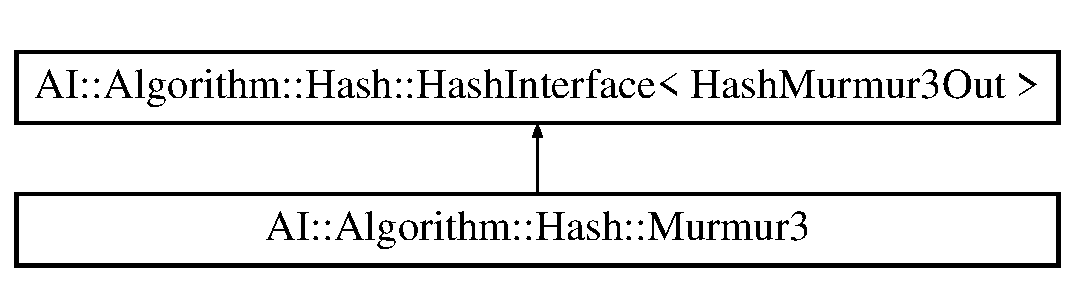
\includegraphics[height=2.000000cm]{classAI_1_1Algorithm_1_1Hash_1_1Murmur3}
\end{center}
\end{figure}
\subsection*{Public Member Functions}
\begin{DoxyCompactItemize}
\item 
virtual \hyperlink{structAI_1_1Algorithm_1_1Hash_1_1HashMurmur3Out}{Hash\+Murmur3\+Out} \hyperlink{classAI_1_1Algorithm_1_1Hash_1_1Murmur3_ab79d4cbd685e34c88077d58e5cacf7a3}{hash} (const \hyperlink{namespaceAI_a9d4bcda82fe0f9aac3c4861e24491581}{A\+I\+::\+B\+Y\+T\+E} $\ast$const byte\+Array, size\+\_\+t len)
\item 
\hypertarget{classAI_1_1Algorithm_1_1Hash_1_1Murmur3_a552acfee5455ac802af225bfd89d80db}{virtual \hyperlink{structAI_1_1Algorithm_1_1Hash_1_1HashMurmur3Out}{Hash\+Murmur3\+Out} {\bfseries hash} (const vector$<$ \hyperlink{namespaceAI_a9d4bcda82fe0f9aac3c4861e24491581}{A\+I\+::\+B\+Y\+T\+E} $>$ \&byte\+Array)}\label{classAI_1_1Algorithm_1_1Hash_1_1Murmur3_a552acfee5455ac802af225bfd89d80db}

\end{DoxyCompactItemize}


\subsection{Detailed Description}
\hyperlink{classAI_1_1Algorithm_1_1Hash_1_1Murmur3}{Murmur3} hash encapsulated. 

\subsection{Member Function Documentation}
\hypertarget{classAI_1_1Algorithm_1_1Hash_1_1Murmur3_ab79d4cbd685e34c88077d58e5cacf7a3}{\index{A\+I\+::\+Algorithm\+::\+Hash\+::\+Murmur3@{A\+I\+::\+Algorithm\+::\+Hash\+::\+Murmur3}!hash@{hash}}
\index{hash@{hash}!A\+I\+::\+Algorithm\+::\+Hash\+::\+Murmur3@{A\+I\+::\+Algorithm\+::\+Hash\+::\+Murmur3}}
\subsubsection[{hash}]{\setlength{\rightskip}{0pt plus 5cm}{\bf Hash\+Murmur3\+Out} A\+I\+::\+Algorithm\+::\+Hash\+::\+Murmur3\+::hash (
\begin{DoxyParamCaption}
\item[{const {\bf A\+I\+::\+B\+Y\+T\+E} $\ast$const}]{byte\+Array, }
\item[{size\+\_\+t}]{len}
\end{DoxyParamCaption}
)\hspace{0.3cm}{\ttfamily [virtual]}}}\label{classAI_1_1Algorithm_1_1Hash_1_1Murmur3_ab79d4cbd685e34c88077d58e5cacf7a3}

\begin{DoxyParams}{Parameters}
{\em byte\+Array} & \\
\hline
{\em len} & \\
\hline
\end{DoxyParams}
\begin{DoxyReturn}{Returns}
h(byte\+Array) 
\end{DoxyReturn}


Implements \hyperlink{classAI_1_1Algorithm_1_1Hash_1_1HashInterface_ae31d650fd044e3ef372cae18a422e0d9}{A\+I\+::\+Algorithm\+::\+Hash\+::\+Hash\+Interface$<$ Hash\+Murmur3\+Out $>$}.



The documentation for this class was generated from the following files\+:\begin{DoxyCompactItemize}
\item 
Algorithms/\+Hash/Hash\+Murmur3.\+h\item 
Algorithms/\+Hash/Hash\+Murmur3.\+cpp\end{DoxyCompactItemize}

\hypertarget{structNDimensionalVector}{\section{N\-Dimensional\-Vector$<$ dim, D $>$ Struct Template Reference}
\label{structNDimensionalVector}\index{N\-Dimensional\-Vector$<$ dim, D $>$@{N\-Dimensional\-Vector$<$ dim, D $>$}}
}


{\ttfamily \#include $<$N\-Dimensional\-Vector.\-h$>$}

\subsection*{Public Types}
\begin{DoxyCompactItemize}
\item 
\hypertarget{structNDimensionalVector_ae933e15c6af2eaed20472909b7030090}{typedef std\-::vector$<$ typename \\*
\hyperlink{structNDimensionalVector}{N\-Dimensional\-Vector}$<$ dim-\/1, D $>$\\*
\-::n\-Array $>$ {\bfseries n\-Array}}\label{structNDimensionalVector_ae933e15c6af2eaed20472909b7030090}

\end{DoxyCompactItemize}


\subsection{Detailed Description}
\subsubsection*{template$<$size\-\_\-t dim, typename D$>$struct N\-Dimensional\-Vector$<$ dim, D $>$}

\hyperlink{structNDimensionalVector}{N\-Dimensional\-Vector}

For representing multidimensional array. 

The documentation for this struct was generated from the following file\-:\begin{DoxyCompactItemize}
\item 
Algorithms/\-Supervised\-Learning/N\-Dimensional\-Vector.\-h\end{DoxyCompactItemize}

\hypertarget{structNDimensionalVector_3_010_00_01D_01_4}{\section{N\+Dimensional\+Vector$<$ 0, D $>$ Struct Template Reference}
\label{structNDimensionalVector_3_010_00_01D_01_4}\index{N\+Dimensional\+Vector$<$ 0, D $>$@{N\+Dimensional\+Vector$<$ 0, D $>$}}
}
\subsection*{Public Types}
\begin{DoxyCompactItemize}
\item 
\hypertarget{structNDimensionalVector_3_010_00_01D_01_4_a1eb07b65caa9aad2b7b20b5b8eefd54a}{typedef D {\bfseries n\+Array}}\label{structNDimensionalVector_3_010_00_01D_01_4_a1eb07b65caa9aad2b7b20b5b8eefd54a}

\end{DoxyCompactItemize}


The documentation for this struct was generated from the following file\+:\begin{DoxyCompactItemize}
\item 
Algorithms/\+Supervised\+Learning/N\+Dimensional\+Vector.\+h\end{DoxyCompactItemize}

\hypertarget{classObservable}{\section{Observable$<$ Notify\-Argument $>$ Class Template Reference}
\label{classObservable}\index{Observable$<$ Notify\-Argument $>$@{Observable$<$ Notify\-Argument $>$}}
}
\subsection*{Public Member Functions}
\begin{DoxyCompactItemize}
\item 
\hypertarget{classObservable_a67b3bb2b5fbf3d29e1366f8e04115b6f}{bool {\bfseries register\-Observer} (\hyperlink{classObserver}{Observer}$<$ Notify\-Argument $>$ \&observable)}\label{classObservable_a67b3bb2b5fbf3d29e1366f8e04115b6f}

\item 
\hypertarget{classObservable_a93fca2f7da9fe212f8e27d299f3feddf}{bool {\bfseries remove\-Observer} (\hyperlink{classObserver}{Observer}$<$ Notify\-Argument $>$ \&observable)}\label{classObservable_a93fca2f7da9fe212f8e27d299f3feddf}

\item 
\hypertarget{classObservable_a48deae3a33d042b8eb2e3a0265b25e64}{void {\bfseries notify\-Observes} (Notify\-Argument \&arg)}\label{classObservable_a48deae3a33d042b8eb2e3a0265b25e64}

\end{DoxyCompactItemize}


The documentation for this class was generated from the following file\-:\begin{DoxyCompactItemize}
\item 
Observable.\-h\end{DoxyCompactItemize}

\hypertarget{classObserver}{\section{Observer$<$ Notify\-Argument $>$ Class Template Reference}
\label{classObserver}\index{Observer$<$ Notify\-Argument $>$@{Observer$<$ Notify\-Argument $>$}}
}
\subsection*{Public Member Functions}
\begin{DoxyCompactItemize}
\item 
\hypertarget{classObserver_ad6a783895b06113b2be6f2dbbeb6bdf4}{virtual void {\bfseries notify} (Notify\-Argument arg)=0}\label{classObserver_ad6a783895b06113b2be6f2dbbeb6bdf4}

\end{DoxyCompactItemize}


The documentation for this class was generated from the following file\-:\begin{DoxyCompactItemize}
\item 
Observer.\-h\end{DoxyCompactItemize}

\hypertarget{classAI_1_1Algorithm_1_1Policy_1_1Policy}{\section{A\-I\-:\-:Algorithm\-:\-:Policy\-:\-:Policy$<$ S, A $>$ Class Template Reference}
\label{classAI_1_1Algorithm_1_1Policy_1_1Policy}\index{A\-I\-::\-Algorithm\-::\-Policy\-::\-Policy$<$ S, A $>$@{A\-I\-::\-Algorithm\-::\-Policy\-::\-Policy$<$ S, A $>$}}
}


Base class for all \hyperlink{classAI_1_1Algorithm_1_1Policy_1_1Policy}{Policy}.  




{\ttfamily \#include $<$Policy.\-h$>$}

Inheritance diagram for A\-I\-:\-:Algorithm\-:\-:Policy\-:\-:Policy$<$ S, A $>$\-:\begin{figure}[H]
\begin{center}
\leavevmode
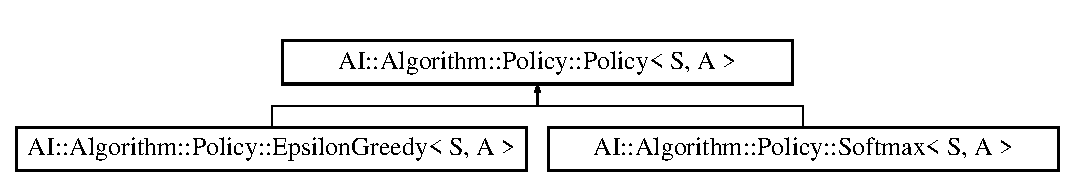
\includegraphics[height=2.000000cm]{classAI_1_1Algorithm_1_1Policy_1_1Policy}
\end{center}
\end{figure}
\subsection*{Public Member Functions}
\begin{DoxyCompactItemize}
\item 
virtual const A \& \hyperlink{classAI_1_1Algorithm_1_1Policy_1_1Policy_a1bd1f511d0f5dce4f4b080232845852c}{get\-Action} (const map$<$ A, A\-I\-::\-F\-L\-O\-A\-T $>$ \&action\-Values, const set$<$ A $>$ \&action\-Set)=0
\end{DoxyCompactItemize}


\subsection{Detailed Description}
\subsubsection*{template$<$class S, class A$>$class A\-I\-::\-Algorithm\-::\-Policy\-::\-Policy$<$ S, A $>$}

Base class for all \hyperlink{classAI_1_1Algorithm_1_1Policy_1_1Policy}{Policy}. 

\hyperlink{classAI_1_1Algorithm_1_1Policy_1_1Policy}{Policy} sets the rule for action selection given a mapping of action to action values and a set of action.


\begin{DoxyTemplParams}{Template Parameters}
{\em S} & State data type. \\
\hline
{\em A} & Action data type. \\
\hline
\end{DoxyTemplParams}


\subsection{Member Function Documentation}
\hypertarget{classAI_1_1Algorithm_1_1Policy_1_1Policy_a1bd1f511d0f5dce4f4b080232845852c}{\index{A\-I\-::\-Algorithm\-::\-Policy\-::\-Policy@{A\-I\-::\-Algorithm\-::\-Policy\-::\-Policy}!get\-Action@{get\-Action}}
\index{get\-Action@{get\-Action}!AI::Algorithm::Policy::Policy@{A\-I\-::\-Algorithm\-::\-Policy\-::\-Policy}}
\subsubsection[{get\-Action}]{\setlength{\rightskip}{0pt plus 5cm}template$<$class S, class A$>$ virtual const A\& {\bf A\-I\-::\-Algorithm\-::\-Policy\-::\-Policy}$<$ S, A $>$\-::get\-Action (
\begin{DoxyParamCaption}
\item[{const map$<$ A, A\-I\-::\-F\-L\-O\-A\-T $>$ \&}]{action\-Values, }
\item[{const set$<$ A $>$ \&}]{action\-Set}
\end{DoxyParamCaption}
)\hspace{0.3cm}{\ttfamily [pure virtual]}}}\label{classAI_1_1Algorithm_1_1Policy_1_1Policy_a1bd1f511d0f5dce4f4b080232845852c}
Returns {\bfseries action} given a mapping of actions and their value and a set of actions.


\begin{DoxyParams}{Parameters}
{\em action\-Values} & a mapping of actions to their corresponding value. \\
\hline
{\em action\-Set} & set of actions. \\
\hline
\end{DoxyParams}
\begin{DoxyReturn}{Returns}
{\bfseries action} given a mapping of actions and their value and a set of actions. 
\end{DoxyReturn}


Implemented in \hyperlink{classAI_1_1Algorithm_1_1Policy_1_1EpsilonGreedy_a00a2dde7f4df14fd046e034694184f65}{A\-I\-::\-Algorithm\-::\-Policy\-::\-Epsilon\-Greedy$<$ S, A $>$}, \hyperlink{classAI_1_1Algorithm_1_1Policy_1_1EpsilonGreedy_a00a2dde7f4df14fd046e034694184f65}{A\-I\-::\-Algorithm\-::\-Policy\-::\-Epsilon\-Greedy$<$ vector$<$ F\-L\-O\-A\-T $>$, vector$<$ F\-L\-O\-A\-T $>$ $>$}, and \hyperlink{classAI_1_1Algorithm_1_1Policy_1_1Softmax_adf507bcadedab2d33e3fcc0059918d19}{A\-I\-::\-Algorithm\-::\-Policy\-::\-Softmax$<$ S, A $>$}.



The documentation for this class was generated from the following file\-:\begin{DoxyCompactItemize}
\item 
Algorithms/\-Policy/Policy.\-h\end{DoxyCompactItemize}

\hypertarget{classAI_1_1Algorithm_1_1QLearning}{\section{A\-I\-:\-:Algorithm\-:\-:Q\-Learning$<$ S, A $>$ Class Template Reference}
\label{classAI_1_1Algorithm_1_1QLearning}\index{A\-I\-::\-Algorithm\-::\-Q\-Learning$<$ S, A $>$@{A\-I\-::\-Algorithm\-::\-Q\-Learning$<$ S, A $>$}}
}


Basic off-\/policy reinforcement learning algorithm.  




{\ttfamily \#include $<$Q\-Learning.\-h$>$}

Inheritance diagram for A\-I\-:\-:Algorithm\-:\-:Q\-Learning$<$ S, A $>$\-:\begin{figure}[H]
\begin{center}
\leavevmode
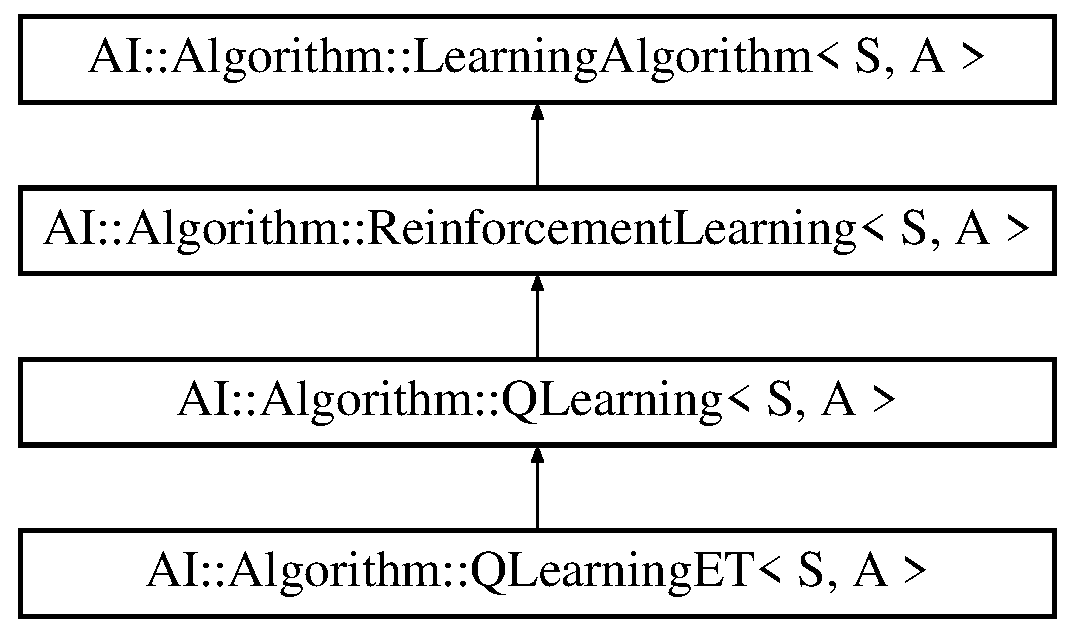
\includegraphics[height=4.000000cm]{classAI_1_1Algorithm_1_1QLearning}
\end{center}
\end{figure}
\subsection*{Public Member Functions}
\begin{DoxyCompactItemize}
\item 
\hyperlink{classAI_1_1Algorithm_1_1QLearning_a182fd44ac6cd6b2474615ce7b98667ce}{Q\-Learning} (\hyperlink{namespaceAI_a41b74884a20833db653dded3918e05c3}{A\-I\-::\-F\-L\-O\-A\-T} step\-Size, \hyperlink{namespaceAI_a41b74884a20833db653dded3918e05c3}{A\-I\-::\-F\-L\-O\-A\-T} discount\-Rate, \hyperlink{classAI_1_1Algorithm_1_1Policy_1_1Policy}{Policy\-::\-Policy}$<$ S, A $>$ \&policy)
\item 
virtual void \hyperlink{classAI_1_1Algorithm_1_1QLearning_a042e1987ce21a94f59603c4cb1eeed82}{update} (const \hyperlink{classAI_1_1StateAction}{State\-Action}$<$ S, A $>$ \&current\-State\-Action, const S \&next\-State, const \hyperlink{namespaceAI_a41b74884a20833db653dded3918e05c3}{A\-I\-::\-F\-L\-O\-A\-T} reward, const set$<$ A $>$ \&action\-Set)
\end{DoxyCompactItemize}
\subsection*{Additional Inherited Members}


\subsection{Detailed Description}
\subsubsection*{template$<$class S, class A$>$class A\-I\-::\-Algorithm\-::\-Q\-Learning$<$ S, A $>$}

Basic off-\/policy reinforcement learning algorithm. 


\begin{DoxyTemplParams}{Template Parameters}
{\em S} & State data type. \\
\hline
{\em A} & Action data type.\\
\hline
\end{DoxyTemplParams}
Different policy is used for learning and action selection. Note that default offline/learning policy is Epsilon\-Greedy 

\subsection{Constructor \& Destructor Documentation}
\hypertarget{classAI_1_1Algorithm_1_1QLearning_a182fd44ac6cd6b2474615ce7b98667ce}{\index{A\-I\-::\-Algorithm\-::\-Q\-Learning@{A\-I\-::\-Algorithm\-::\-Q\-Learning}!Q\-Learning@{Q\-Learning}}
\index{Q\-Learning@{Q\-Learning}!AI::Algorithm::QLearning@{A\-I\-::\-Algorithm\-::\-Q\-Learning}}
\subsubsection[{Q\-Learning}]{\setlength{\rightskip}{0pt plus 5cm}template$<$class S , class A $>$ {\bf A\-I\-::\-Algorithm\-::\-Q\-Learning}$<$ S, A $>$\-::{\bf Q\-Learning} (
\begin{DoxyParamCaption}
\item[{{\bf A\-I\-::\-F\-L\-O\-A\-T}}]{step\-Size, }
\item[{{\bf A\-I\-::\-F\-L\-O\-A\-T}}]{discount\-Rate, }
\item[{{\bf Policy\-::\-Policy}$<$ S, A $>$ \&}]{policy}
\end{DoxyParamCaption}
)}}\label{classAI_1_1Algorithm_1_1QLearning_a182fd44ac6cd6b2474615ce7b98667ce}

\begin{DoxyParams}{Parameters}
{\em step\-Size} & range $[0.0, 1.0]$. High step size means faster learning, but less precise convergence. \\
\hline
{\em discount\-Rate} & range $[0.0, 1.0]$. High discount rate means more consideration of future events. \\
\hline
{\em policy} & online policy, that is policy used for action selection. \\
\hline
\end{DoxyParams}


\subsection{Member Function Documentation}
\hypertarget{classAI_1_1Algorithm_1_1QLearning_a042e1987ce21a94f59603c4cb1eeed82}{\index{A\-I\-::\-Algorithm\-::\-Q\-Learning@{A\-I\-::\-Algorithm\-::\-Q\-Learning}!update@{update}}
\index{update@{update}!AI::Algorithm::QLearning@{A\-I\-::\-Algorithm\-::\-Q\-Learning}}
\subsubsection[{update}]{\setlength{\rightskip}{0pt plus 5cm}template$<$class S , class A $>$ void {\bf A\-I\-::\-Algorithm\-::\-Q\-Learning}$<$ S, A $>$\-::update (
\begin{DoxyParamCaption}
\item[{const {\bf State\-Action}$<$ S, A $>$ \&}]{current\-State\-Action, }
\item[{const S \&}]{next\-State, }
\item[{const {\bf A\-I\-::\-F\-L\-O\-A\-T}}]{reward, }
\item[{const set$<$ A $>$ \&}]{action\-Set}
\end{DoxyParamCaption}
)\hspace{0.3cm}{\ttfamily [virtual]}}}\label{classAI_1_1Algorithm_1_1QLearning_a042e1987ce21a94f59603c4cb1eeed82}
Update the state\-Action map. 
\begin{DoxyParams}{Parameters}
{\em current\-State} & current\-State agent is in. \\
\hline
{\em current\-Action} & action taken by agent by being in current\-State. \\
\hline
{\em next\-State} & next\-State by taking current\-Action in current\-State. \\
\hline
{\em reward} & reward of current\-State\-Action. \\
\hline
{\em action\-Set} & A set of all actions. \\
\hline
\end{DoxyParams}


Reimplemented from \hyperlink{classAI_1_1Algorithm_1_1ReinforcementLearning_a25d7fa245a79e61061436dc0f1db90cb}{A\-I\-::\-Algorithm\-::\-Reinforcement\-Learning$<$ S, A $>$}.



Reimplemented in \hyperlink{classAI_1_1Algorithm_1_1QLearningET_a9a245dcb3ca8f26b37e5a6daa6d4a898}{A\-I\-::\-Algorithm\-::\-Q\-Learning\-E\-T$<$ S, A $>$}.



The documentation for this class was generated from the following file\-:\begin{DoxyCompactItemize}
\item 
Algorithms/\-Reinforcement\-Learning/Q\-Learning.\-h\end{DoxyCompactItemize}

\hypertarget{classAI_1_1Algorithm_1_1QLearningETGD}{\section{A\-I\-:\-:Algorithm\-:\-:Q\-Learning\-E\-T\-G\-D Class Reference}
\label{classAI_1_1Algorithm_1_1QLearningETGD}\index{A\-I\-::\-Algorithm\-::\-Q\-Learning\-E\-T\-G\-D@{A\-I\-::\-Algorithm\-::\-Q\-Learning\-E\-T\-G\-D}}
}
Inheritance diagram for A\-I\-:\-:Algorithm\-:\-:Q\-Learning\-E\-T\-G\-D\-:\begin{figure}[H]
\begin{center}
\leavevmode
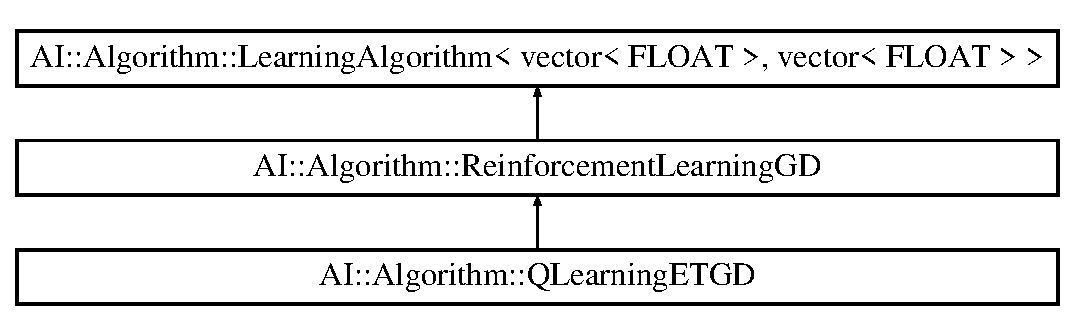
\includegraphics[height=3.000000cm]{classAI_1_1Algorithm_1_1QLearningETGD}
\end{center}
\end{figure}
\subsection*{Public Member Functions}
\begin{DoxyCompactItemize}
\item 
\hypertarget{classAI_1_1Algorithm_1_1QLearningETGD_af809fcbeb278128ba61f6f0249675d46}{{\bfseries Q\-Learning\-E\-T\-G\-D} (\hyperlink{classAI_1_1Algorithm_1_1TileCode}{Tile\-Code} \&tile\-Code, A\-I\-::\-F\-L\-O\-A\-T step\-Size, A\-I\-::\-F\-L\-O\-A\-T discount\-Rate, A\-I\-::\-F\-L\-O\-A\-T lambda, \hyperlink{classAI_1_1Algorithm_1_1Policy}{Policy\-S\-L} \&control\-Policy)}\label{classAI_1_1Algorithm_1_1QLearningETGD_af809fcbeb278128ba61f6f0249675d46}

\end{DoxyCompactItemize}
\subsection*{Additional Inherited Members}


The documentation for this class was generated from the following file\-:\begin{DoxyCompactItemize}
\item 
Algorithms/\-Supervised\-Learning/Q\-Learning\-E\-T\-G\-D.\-h\end{DoxyCompactItemize}

\hypertarget{classAI_1_1Algorithm_1_1QLearningETWatkins}{\section{A\-I\-:\-:Algorithm\-:\-:Q\-Learning\-E\-T\-Watkins$<$ S, A $>$ Class Template Reference}
\label{classAI_1_1Algorithm_1_1QLearningETWatkins}\index{A\-I\-::\-Algorithm\-::\-Q\-Learning\-E\-T\-Watkins$<$ S, A $>$@{A\-I\-::\-Algorithm\-::\-Q\-Learning\-E\-T\-Watkins$<$ S, A $>$}}
}


{\ttfamily \#include $<$Q\-Learning\-E\-T\-Watkins.\-h$>$}

Inheritance diagram for A\-I\-:\-:Algorithm\-:\-:Q\-Learning\-E\-T\-Watkins$<$ S, A $>$\-:\begin{figure}[H]
\begin{center}
\leavevmode
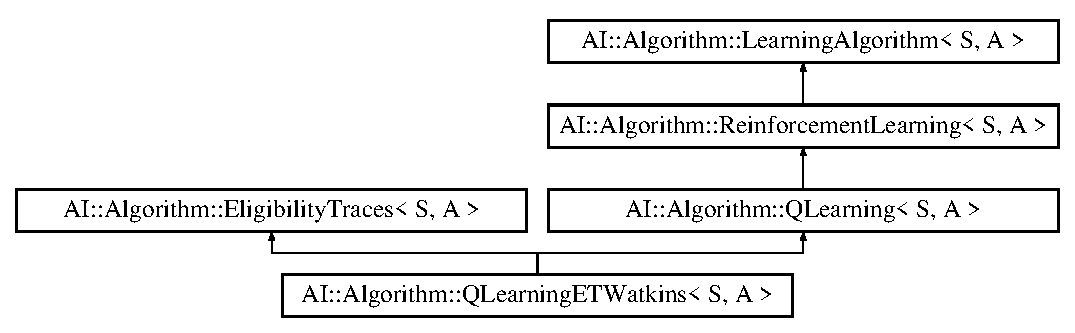
\includegraphics[height=4.000000cm]{classAI_1_1Algorithm_1_1QLearningETWatkins}
\end{center}
\end{figure}
\subsection*{Public Member Functions}
\begin{DoxyCompactItemize}
\item 
\hypertarget{classAI_1_1Algorithm_1_1QLearningETWatkins_a0304d02e8ea871414b23e6201e1f1dcc}{{\bfseries Q\-Learning\-E\-T\-Watkins} (\hyperlink{namespaceAI_a41b74884a20833db653dded3918e05c3}{A\-I\-::\-F\-L\-O\-A\-T} step\-Size, \hyperlink{namespaceAI_a41b74884a20833db653dded3918e05c3}{A\-I\-::\-F\-L\-O\-A\-T} discount\-Rate, \hyperlink{classAI_1_1Algorithm_1_1Policy_1_1Policy}{Policy\-::\-Policy}$<$ S, A $>$ \&policy, \hyperlink{namespaceAI_a41b74884a20833db653dded3918e05c3}{A\-I\-::\-F\-L\-O\-A\-T} lambda)}\label{classAI_1_1Algorithm_1_1QLearningETWatkins_a0304d02e8ea871414b23e6201e1f1dcc}

\item 
virtual void \hyperlink{classAI_1_1Algorithm_1_1QLearningETWatkins_a5cbad8c16dfbf6fe72c85fe5c8c4e273}{update} (const \hyperlink{classAI_1_1StateAction}{State\-Action}$<$ S, A $>$ \&current\-State\-Action, const S \&next\-State, const \hyperlink{namespaceAI_a41b74884a20833db653dded3918e05c3}{A\-I\-::\-F\-L\-O\-A\-T} current\-State\-Action\-Value, const set$<$ A $>$ \&action\-Set)
\end{DoxyCompactItemize}
\subsection*{Additional Inherited Members}


\subsection{Detailed Description}
\subsubsection*{template$<$class S, class A$>$class A\-I\-::\-Algorithm\-::\-Q\-Learning\-E\-T\-Watkins$<$ S, A $>$}

\hyperlink{classAI_1_1Algorithm_1_1QLearningETWatkins}{Q\-Learning\-E\-T\-Watkins} \begin{DoxySeeAlso}{See Also}
\hyperlink{classAI_1_1Algorithm_1_1QLearning}{Q\-Learning} 

\hyperlink{classAI_1_1Algorithm_1_1EligibilityTraces}{Eligibility\-Traces} 
\end{DoxySeeAlso}


\subsection{Member Function Documentation}
\hypertarget{classAI_1_1Algorithm_1_1QLearningETWatkins_a5cbad8c16dfbf6fe72c85fe5c8c4e273}{\index{A\-I\-::\-Algorithm\-::\-Q\-Learning\-E\-T\-Watkins@{A\-I\-::\-Algorithm\-::\-Q\-Learning\-E\-T\-Watkins}!update@{update}}
\index{update@{update}!AI::Algorithm::QLearningETWatkins@{A\-I\-::\-Algorithm\-::\-Q\-Learning\-E\-T\-Watkins}}
\subsubsection[{update}]{\setlength{\rightskip}{0pt plus 5cm}template$<$class S , class A $>$ void {\bf A\-I\-::\-Algorithm\-::\-Q\-Learning\-E\-T\-Watkins}$<$ S, A $>$\-::update (
\begin{DoxyParamCaption}
\item[{const {\bf State\-Action}$<$ S, A $>$ \&}]{current\-State\-Action, }
\item[{const S \&}]{next\-State, }
\item[{const {\bf A\-I\-::\-F\-L\-O\-A\-T}}]{current\-State\-Action\-Value, }
\item[{const set$<$ A $>$ \&}]{action\-Set}
\end{DoxyParamCaption}
)\hspace{0.3cm}{\ttfamily [virtual]}}}\label{classAI_1_1Algorithm_1_1QLearningETWatkins_a5cbad8c16dfbf6fe72c85fe5c8c4e273}
Update the state\-Action map. 
\begin{DoxyParams}{Parameters}
{\em current\-State} & \\
\hline
{\em current\-Action} & \\
\hline
{\em next\-State} & \\
\hline
{\em current\-State\-Action\-Value} & Value of current\-State and current\-Action. \\
\hline
{\em state\-Action} & A map of \hyperlink{classAI_1_1StateAction}{State\-Action} to Value. \\
\hline
{\em action\-Set} & A set of all actions. \\
\hline
\end{DoxyParams}
\begin{DoxyReturn}{Returns}
next action to be executed. 
\end{DoxyReturn}


Reimplemented from \hyperlink{classAI_1_1Algorithm_1_1QLearning_a042e1987ce21a94f59603c4cb1eeed82}{A\-I\-::\-Algorithm\-::\-Q\-Learning$<$ S, A $>$}.



The documentation for this class was generated from the following file\-:\begin{DoxyCompactItemize}
\item 
Algorithms/\-Reinforcement\-Learning/Q\-Learning\-E\-T\-Watkins.\-h\end{DoxyCompactItemize}

\hypertarget{classAI_1_1Algorithm_1_1ReinforcementLearning}{\section{A\-I\-:\-:Algorithm\-:\-:Reinforcement\-Learning$<$ S, A $>$ Class Template Reference}
\label{classAI_1_1Algorithm_1_1ReinforcementLearning}\index{A\-I\-::\-Algorithm\-::\-Reinforcement\-Learning$<$ S, A $>$@{A\-I\-::\-Algorithm\-::\-Reinforcement\-Learning$<$ S, A $>$}}
}


Abstract class for all Reinforcement learning algorithms.  




{\ttfamily \#include $<$Reinforcement\-Learning.\-h$>$}

Inheritance diagram for A\-I\-:\-:Algorithm\-:\-:Reinforcement\-Learning$<$ S, A $>$\-:\begin{figure}[H]
\begin{center}
\leavevmode
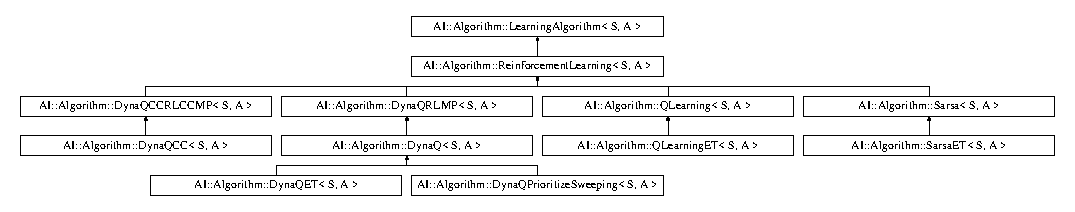
\includegraphics[height=2.397260cm]{classAI_1_1Algorithm_1_1ReinforcementLearning}
\end{center}
\end{figure}
\subsection*{Public Member Functions}
\begin{DoxyCompactItemize}
\item 
\hyperlink{classAI_1_1Algorithm_1_1ReinforcementLearning_a4d182d91c68aef838b80843acd044b1e}{Reinforcement\-Learning} (\hyperlink{namespaceAI_a41b74884a20833db653dded3918e05c3}{A\-I\-::\-F\-L\-O\-A\-T} step\-Size, \hyperlink{namespaceAI_a41b74884a20833db653dded3918e05c3}{A\-I\-::\-F\-L\-O\-A\-T} discount\-Rate, \hyperlink{classAI_1_1Algorithm_1_1Policy_1_1Policy}{Policy\-::\-Policy}$<$ S, A $>$ \&policy)
\item 
A \hyperlink{classAI_1_1Algorithm_1_1ReinforcementLearning_ad1d8a8ebb47fb71a53b15b770795e286}{arg\-Max} (const S \&state, const set$<$ A $>$ \&action\-Set) const 
\item 
virtual \hyperlink{namespaceAI_a41b74884a20833db653dded3918e05c3}{A\-I\-::\-F\-L\-O\-A\-T} \hyperlink{classAI_1_1Algorithm_1_1ReinforcementLearning_a04edb957e23dde9c6733668ad844c32b}{get\-Discount\-Rate} () const 
\item 
virtual void \hyperlink{classAI_1_1Algorithm_1_1ReinforcementLearning_a1fc1e11a3ddb4377c4d6813a95ce87f4}{set\-Discount\-Rate} (\hyperlink{namespaceAI_a41b74884a20833db653dded3918e05c3}{A\-I\-::\-F\-L\-O\-A\-T} discount\-Rate)
\item 
virtual \hyperlink{namespaceAI_a41b74884a20833db653dded3918e05c3}{A\-I\-::\-F\-L\-O\-A\-T} \hyperlink{classAI_1_1Algorithm_1_1ReinforcementLearning_a13e6c161a33644183d3d357971eeaaf5}{get\-Step\-Size} () const 
\item 
virtual void \hyperlink{classAI_1_1Algorithm_1_1ReinforcementLearning_a04932645faa6c385e4c587f7f845b484}{set\-Step\-Size} (\hyperlink{namespaceAI_a41b74884a20833db653dded3918e05c3}{A\-I\-::\-F\-L\-O\-A\-T} step\-Size)
\item 
virtual void \hyperlink{classAI_1_1Algorithm_1_1ReinforcementLearning_aa45b49ec954f6934df4d541b70076bd6}{back\-Up\-State\-Action\-Pair} (const \hyperlink{classAI_1_1StateAction}{State\-Action}$<$ S, A $>$ \&current\-State\-Action, const \hyperlink{namespaceAI_a41b74884a20833db653dded3918e05c3}{A\-I\-::\-F\-L\-O\-A\-T} reward, const \hyperlink{classAI_1_1StateAction}{State\-Action}$<$ S, A $>$ \&next\-State\-Action\-Pair)
\item 
const A \& \hyperlink{classAI_1_1Algorithm_1_1ReinforcementLearning_a9f31822bf51b07d17b31d7683d7e25a2}{get\-Learning\-Action} (const S \&current\-State, const set$<$ A $>$ \&action\-Set)
\item 
virtual \hyperlink{namespaceAI_a41b74884a20833db653dded3918e05c3}{A\-I\-::\-F\-L\-O\-A\-T} \hyperlink{classAI_1_1Algorithm_1_1ReinforcementLearning_ad078677d92b33df4ae7d3c78e040b766}{get\-State\-Action\-Value} (const \hyperlink{classAI_1_1StateAction}{State\-Action}$<$ S, A $>$ \&state\-Action)
\item 
virtual void \hyperlink{classAI_1_1Algorithm_1_1ReinforcementLearning_a5d576410235e5099f153d21f20a8e5af}{set\-State\-Action\-Value} (const \hyperlink{classAI_1_1StateAction}{State\-Action}$<$ S, A $>$ \&state\-Action, const \hyperlink{namespaceAI_a41b74884a20833db653dded3918e05c3}{A\-I\-::\-F\-L\-O\-A\-T} \&reward)
\item 
const \hyperlink{classAI_1_1StateActionPairContainer}{State\-Action\-Pair\-Container}\\*
$<$ S, A $>$ \& \hyperlink{classAI_1_1Algorithm_1_1ReinforcementLearning_a6b5fe1be9629bf5574d32ae4eeec33f5}{get\-State\-Action\-Pair\-Container} () const 
\item 
void \hyperlink{classAI_1_1Algorithm_1_1ReinforcementLearning_ad889f5f5949cac39d121f57e3027ad0c}{set\-State\-Action\-Pair\-Container} (const \hyperlink{classAI_1_1StateActionPairContainer}{State\-Action\-Pair\-Container}$<$ S, A $>$ \&state\-Action\-Pair\-Container)
\item 
virtual void \hyperlink{classAI_1_1Algorithm_1_1ReinforcementLearning_a25d7fa245a79e61061436dc0f1db90cb}{update} (const \hyperlink{classAI_1_1StateAction}{State\-Action}$<$ S, A $>$ \&current\-State\-Action, const S \&next\-State, const \hyperlink{namespaceAI_a41b74884a20833db653dded3918e05c3}{A\-I\-::\-F\-L\-O\-A\-T} reward, const set$<$ A $>$ \&action\-Set)
\item 
virtual const A \& \hyperlink{classAI_1_1Algorithm_1_1ReinforcementLearning_acb89c1734df6658a422af510b7c36377}{get\-Action} (const S \&current\-State, const set$<$ A $>$ \&action\-Set)
\end{DoxyCompactItemize}
\subsection*{Protected Member Functions}
\begin{DoxyCompactItemize}
\item 
\hypertarget{classAI_1_1Algorithm_1_1ReinforcementLearning_a3efc892a8b36ee3f878c86d15f30883f}{void {\bfseries \-\_\-build\-Action\-Value\-Map} (const set$<$ A $>$ \&action\-Set, const S \&current\-State, map$<$ A, \hyperlink{namespaceAI_a41b74884a20833db653dded3918e05c3}{A\-I\-::\-F\-L\-O\-A\-T} $>$ \&action\-Value\-Map)}\label{classAI_1_1Algorithm_1_1ReinforcementLearning_a3efc892a8b36ee3f878c86d15f30883f}

\end{DoxyCompactItemize}
\subsection*{Protected Attributes}
\begin{DoxyCompactItemize}
\item 
\hypertarget{classAI_1_1Algorithm_1_1ReinforcementLearning_ae8a4204e547054e55542e6f7de4b5dc1}{\hyperlink{namespaceAI_a41b74884a20833db653dded3918e05c3}{A\-I\-::\-F\-L\-O\-A\-T} {\bfseries \-\_\-step\-Size}}\label{classAI_1_1Algorithm_1_1ReinforcementLearning_ae8a4204e547054e55542e6f7de4b5dc1}

\item 
\hypertarget{classAI_1_1Algorithm_1_1ReinforcementLearning_af72ecd83332f502a73f9c5636f433de2}{\hyperlink{namespaceAI_a41b74884a20833db653dded3918e05c3}{A\-I\-::\-F\-L\-O\-A\-T} {\bfseries \-\_\-discount\-Rate}}\label{classAI_1_1Algorithm_1_1ReinforcementLearning_af72ecd83332f502a73f9c5636f433de2}

\item 
\hypertarget{classAI_1_1Algorithm_1_1ReinforcementLearning_aee3318af6590363309fdd04fb9eeebe5}{\hyperlink{classAI_1_1StateActionPairContainer}{State\-Action\-Pair\-Container}$<$ S, A $>$ {\bfseries \-\_\-state\-Action\-Pair\-Container}}\label{classAI_1_1Algorithm_1_1ReinforcementLearning_aee3318af6590363309fdd04fb9eeebe5}

\item 
\hypertarget{classAI_1_1Algorithm_1_1ReinforcementLearning_aa6cddd34af5d8565ea71796434dc17af}{boost\-::shared\-\_\-mutex {\bfseries \-\_\-general\-Lock}}\label{classAI_1_1Algorithm_1_1ReinforcementLearning_aa6cddd34af5d8565ea71796434dc17af}

\item 
\hypertarget{classAI_1_1Algorithm_1_1ReinforcementLearning_a365513e575cf60c0ae6fd5dfcfc54913}{boost\-::shared\-\_\-mutex {\bfseries \-\_\-container\-Lock}}\label{classAI_1_1Algorithm_1_1ReinforcementLearning_a365513e575cf60c0ae6fd5dfcfc54913}

\item 
\hypertarget{classAI_1_1Algorithm_1_1ReinforcementLearning_acc5503fcb31fb030be0c9d302517adcc}{boost\-::shared\-\_\-mutex {\bfseries \-\_\-step\-Size\-Lock}}\label{classAI_1_1Algorithm_1_1ReinforcementLearning_acc5503fcb31fb030be0c9d302517adcc}

\item 
\hypertarget{classAI_1_1Algorithm_1_1ReinforcementLearning_aaa369f14f7f9b9ddb0bf8efb2b8363dd}{boost\-::shared\-\_\-mutex {\bfseries \-\_\-discount\-Rate\-Lock}}\label{classAI_1_1Algorithm_1_1ReinforcementLearning_aaa369f14f7f9b9ddb0bf8efb2b8363dd}

\end{DoxyCompactItemize}
\subsection*{Additional Inherited Members}


\subsection{Detailed Description}
\subsubsection*{template$<$class S, class A$>$class A\-I\-::\-Algorithm\-::\-Reinforcement\-Learning$<$ S, A $>$}

Abstract class for all Reinforcement learning algorithms. 


\begin{DoxyTemplParams}{Template Parameters}
{\em S} & state data type. \\
\hline
{\em A} & action data type.\\
\hline
\end{DoxyTemplParams}
All reinforcement algorithm inherit from this class. 

\subsection{Constructor \& Destructor Documentation}
\hypertarget{classAI_1_1Algorithm_1_1ReinforcementLearning_a4d182d91c68aef838b80843acd044b1e}{\index{A\-I\-::\-Algorithm\-::\-Reinforcement\-Learning@{A\-I\-::\-Algorithm\-::\-Reinforcement\-Learning}!Reinforcement\-Learning@{Reinforcement\-Learning}}
\index{Reinforcement\-Learning@{Reinforcement\-Learning}!AI::Algorithm::ReinforcementLearning@{A\-I\-::\-Algorithm\-::\-Reinforcement\-Learning}}
\subsubsection[{Reinforcement\-Learning}]{\setlength{\rightskip}{0pt plus 5cm}template$<$class S , class A $>$ {\bf A\-I\-::\-Algorithm\-::\-Reinforcement\-Learning}$<$ S, A $>$\-::{\bf Reinforcement\-Learning} (
\begin{DoxyParamCaption}
\item[{{\bf A\-I\-::\-F\-L\-O\-A\-T}}]{step\-Size, }
\item[{{\bf A\-I\-::\-F\-L\-O\-A\-T}}]{discount\-Rate, }
\item[{{\bf Policy\-::\-Policy}$<$ S, A $>$ \&}]{policy}
\end{DoxyParamCaption}
)}}\label{classAI_1_1Algorithm_1_1ReinforcementLearning_a4d182d91c68aef838b80843acd044b1e}

\begin{DoxyParams}{Parameters}
{\em step\-Size} & range $[0.0, 1.0]$. High step size means faster learning, but less precise convergence. \\
\hline
{\em discount\-Rate} & range $[0.0, 1.0]$. High discount rate means more consideration of future events. \\
\hline
{\em policy} & online policy, that is policy used for action selection. \\
\hline
\end{DoxyParams}


\subsection{Member Function Documentation}
\hypertarget{classAI_1_1Algorithm_1_1ReinforcementLearning_ad1d8a8ebb47fb71a53b15b770795e286}{\index{A\-I\-::\-Algorithm\-::\-Reinforcement\-Learning@{A\-I\-::\-Algorithm\-::\-Reinforcement\-Learning}!arg\-Max@{arg\-Max}}
\index{arg\-Max@{arg\-Max}!AI::Algorithm::ReinforcementLearning@{A\-I\-::\-Algorithm\-::\-Reinforcement\-Learning}}
\subsubsection[{arg\-Max}]{\setlength{\rightskip}{0pt plus 5cm}template$<$class S , class A $>$ A {\bf A\-I\-::\-Algorithm\-::\-Reinforcement\-Learning}$<$ S, A $>$\-::arg\-Max (
\begin{DoxyParamCaption}
\item[{const S \&}]{state, }
\item[{const set$<$ A $>$ \&}]{action\-Set}
\end{DoxyParamCaption}
) const}}\label{classAI_1_1Algorithm_1_1ReinforcementLearning_ad1d8a8ebb47fb71a53b15b770795e286}
Returns the action that will most \char`\"{}likely\char`\"{} gives the highest reward from the current state. 
\begin{DoxyParams}{Parameters}
{\em state} & the state to apply the arg\-Max to. \\
\hline
{\em state\-Action} & map of \hyperlink{classAI_1_1StateAction}{State\-Action} to value. \\
\hline
{\em action\-Set} & a set of possible actions. \\
\hline
\end{DoxyParams}
\begin{DoxyReturn}{Returns}
the action that will \char`\"{}likely\char`\"{} gives the highest reward. 
\end{DoxyReturn}
\hypertarget{classAI_1_1Algorithm_1_1ReinforcementLearning_aa45b49ec954f6934df4d541b70076bd6}{\index{A\-I\-::\-Algorithm\-::\-Reinforcement\-Learning@{A\-I\-::\-Algorithm\-::\-Reinforcement\-Learning}!back\-Up\-State\-Action\-Pair@{back\-Up\-State\-Action\-Pair}}
\index{back\-Up\-State\-Action\-Pair@{back\-Up\-State\-Action\-Pair}!AI::Algorithm::ReinforcementLearning@{A\-I\-::\-Algorithm\-::\-Reinforcement\-Learning}}
\subsubsection[{back\-Up\-State\-Action\-Pair}]{\setlength{\rightskip}{0pt plus 5cm}template$<$class S , class A $>$ void {\bf A\-I\-::\-Algorithm\-::\-Reinforcement\-Learning}$<$ S, A $>$\-::back\-Up\-State\-Action\-Pair (
\begin{DoxyParamCaption}
\item[{const {\bf State\-Action}$<$ S, A $>$ \&}]{current\-State\-Action, }
\item[{const {\bf A\-I\-::\-F\-L\-O\-A\-T}}]{reward, }
\item[{const {\bf State\-Action}$<$ S, A $>$ \&}]{next\-State\-Action\-Pair}
\end{DoxyParamCaption}
)\hspace{0.3cm}{\ttfamily [virtual]}}}\label{classAI_1_1Algorithm_1_1ReinforcementLearning_aa45b49ec954f6934df4d541b70076bd6}
Does the main back up for all Temporal difference\-: $ Q[S, A] \leftarrow Q[S, A] + \alpha\times [R + \gamma \times max_{A'}Q[S', A'] - Q[S, A] ]$ 
\begin{DoxyParams}{Parameters}
{\em current\-State\-Action} & $(S, A)$, current state-\/action pair. \\
\hline
{\em reward} & $R$, reward after $(S, A)$. \\
\hline
{\em next\-State\-Action\-Pair} & $(S', A')$, next state-\/action pair. \\
\hline
\end{DoxyParams}


Reimplemented in \hyperlink{classAI_1_1Algorithm_1_1DynaQRLMP_a7b3b5f3706744290b12c19f786e5e4e4}{A\-I\-::\-Algorithm\-::\-Dyna\-Q\-R\-L\-M\-P$<$ S, A $>$}, and \hyperlink{classAI_1_1Algorithm_1_1DynaQCCRLCCMP_aebff9b81db5bd2ae33bd3d6662539bc0}{A\-I\-::\-Algorithm\-::\-Dyna\-Q\-C\-C\-R\-L\-C\-C\-M\-P$<$ S, A $>$}.

\hypertarget{classAI_1_1Algorithm_1_1ReinforcementLearning_acb89c1734df6658a422af510b7c36377}{\index{A\-I\-::\-Algorithm\-::\-Reinforcement\-Learning@{A\-I\-::\-Algorithm\-::\-Reinforcement\-Learning}!get\-Action@{get\-Action}}
\index{get\-Action@{get\-Action}!AI::Algorithm::ReinforcementLearning@{A\-I\-::\-Algorithm\-::\-Reinforcement\-Learning}}
\subsubsection[{get\-Action}]{\setlength{\rightskip}{0pt plus 5cm}template$<$class S , class A $>$ const A \& {\bf A\-I\-::\-Algorithm\-::\-Reinforcement\-Learning}$<$ S, A $>$\-::get\-Action (
\begin{DoxyParamCaption}
\item[{const S \&}]{state, }
\item[{const set$<$ A $>$ \&}]{action\-Set}
\end{DoxyParamCaption}
)\hspace{0.3cm}{\ttfamily [virtual]}}}\label{classAI_1_1Algorithm_1_1ReinforcementLearning_acb89c1734df6658a422af510b7c36377}
A policy that varies between algorithms. 

Implements \hyperlink{classAI_1_1Algorithm_1_1LearningAlgorithm_afeca4eded9bc0a02312ccbbfd05f8daa}{A\-I\-::\-Algorithm\-::\-Learning\-Algorithm$<$ S, A $>$}.

\hypertarget{classAI_1_1Algorithm_1_1ReinforcementLearning_a04edb957e23dde9c6733668ad844c32b}{\index{A\-I\-::\-Algorithm\-::\-Reinforcement\-Learning@{A\-I\-::\-Algorithm\-::\-Reinforcement\-Learning}!get\-Discount\-Rate@{get\-Discount\-Rate}}
\index{get\-Discount\-Rate@{get\-Discount\-Rate}!AI::Algorithm::ReinforcementLearning@{A\-I\-::\-Algorithm\-::\-Reinforcement\-Learning}}
\subsubsection[{get\-Discount\-Rate}]{\setlength{\rightskip}{0pt plus 5cm}template$<$class S , class A $>$ {\bf A\-I\-::\-F\-L\-O\-A\-T} {\bf A\-I\-::\-Algorithm\-::\-Reinforcement\-Learning}$<$ S, A $>$\-::get\-Discount\-Rate (
\begin{DoxyParamCaption}
{}
\end{DoxyParamCaption}
) const\hspace{0.3cm}{\ttfamily [inline]}, {\ttfamily [virtual]}}}\label{classAI_1_1Algorithm_1_1ReinforcementLearning_a04edb957e23dde9c6733668ad844c32b}
\begin{DoxyReturn}{Returns}
current discount rate. 
\end{DoxyReturn}
\hypertarget{classAI_1_1Algorithm_1_1ReinforcementLearning_a9f31822bf51b07d17b31d7683d7e25a2}{\index{A\-I\-::\-Algorithm\-::\-Reinforcement\-Learning@{A\-I\-::\-Algorithm\-::\-Reinforcement\-Learning}!get\-Learning\-Action@{get\-Learning\-Action}}
\index{get\-Learning\-Action@{get\-Learning\-Action}!AI::Algorithm::ReinforcementLearning@{A\-I\-::\-Algorithm\-::\-Reinforcement\-Learning}}
\subsubsection[{get\-Learning\-Action}]{\setlength{\rightskip}{0pt plus 5cm}template$<$class S , class A $>$ const A \& {\bf A\-I\-::\-Algorithm\-::\-Reinforcement\-Learning}$<$ S, A $>$\-::get\-Learning\-Action (
\begin{DoxyParamCaption}
\item[{const S \&}]{current\-State, }
\item[{const set$<$ A $>$ \&}]{action\-Set}
\end{DoxyParamCaption}
)\hspace{0.3cm}{\ttfamily [inline]}}}\label{classAI_1_1Algorithm_1_1ReinforcementLearning_a9f31822bf51b07d17b31d7683d7e25a2}
Get Action with respect to learning/offline policy. 
\begin{DoxyParams}{Parameters}
{\em current\-State} & state to acquire state-\/action values from. \\
\hline
{\em action\-Set} & Set of actions. \\
\hline
\end{DoxyParams}
\begin{DoxyReturn}{Returns}
Action with respect to learning/offline policy. 
\end{DoxyReturn}
\hypertarget{classAI_1_1Algorithm_1_1ReinforcementLearning_a6b5fe1be9629bf5574d32ae4eeec33f5}{\index{A\-I\-::\-Algorithm\-::\-Reinforcement\-Learning@{A\-I\-::\-Algorithm\-::\-Reinforcement\-Learning}!get\-State\-Action\-Pair\-Container@{get\-State\-Action\-Pair\-Container}}
\index{get\-State\-Action\-Pair\-Container@{get\-State\-Action\-Pair\-Container}!AI::Algorithm::ReinforcementLearning@{A\-I\-::\-Algorithm\-::\-Reinforcement\-Learning}}
\subsubsection[{get\-State\-Action\-Pair\-Container}]{\setlength{\rightskip}{0pt plus 5cm}template$<$class S , class A $>$ const {\bf A\-I\-::\-State\-Action\-Pair\-Container}$<$ S, A $>$ \& {\bf A\-I\-::\-Algorithm\-::\-Reinforcement\-Learning}$<$ S, A $>$\-::get\-State\-Action\-Pair\-Container (
\begin{DoxyParamCaption}
{}
\end{DoxyParamCaption}
) const\hspace{0.3cm}{\ttfamily [inline]}}}\label{classAI_1_1Algorithm_1_1ReinforcementLearning_a6b5fe1be9629bf5574d32ae4eeec33f5}
\begin{DoxyReturn}{Returns}
state-\/action pair container. 
\end{DoxyReturn}
\hypertarget{classAI_1_1Algorithm_1_1ReinforcementLearning_ad078677d92b33df4ae7d3c78e040b766}{\index{A\-I\-::\-Algorithm\-::\-Reinforcement\-Learning@{A\-I\-::\-Algorithm\-::\-Reinforcement\-Learning}!get\-State\-Action\-Value@{get\-State\-Action\-Value}}
\index{get\-State\-Action\-Value@{get\-State\-Action\-Value}!AI::Algorithm::ReinforcementLearning@{A\-I\-::\-Algorithm\-::\-Reinforcement\-Learning}}
\subsubsection[{get\-State\-Action\-Value}]{\setlength{\rightskip}{0pt plus 5cm}template$<$class S , class A $>$ {\bf A\-I\-::\-F\-L\-O\-A\-T} {\bf A\-I\-::\-Algorithm\-::\-Reinforcement\-Learning}$<$ S, A $>$\-::get\-State\-Action\-Value (
\begin{DoxyParamCaption}
\item[{const {\bf State\-Action}$<$ S, A $>$ \&}]{state\-Action}
\end{DoxyParamCaption}
)\hspace{0.3cm}{\ttfamily [virtual]}}}\label{classAI_1_1Algorithm_1_1ReinforcementLearning_ad078677d92b33df4ae7d3c78e040b766}

\begin{DoxyParams}{Parameters}
{\em state\-Action} & to acquire a value of. \\
\hline
\end{DoxyParams}
\begin{DoxyReturn}{Returns}
the value of state-\/action pair. 
\end{DoxyReturn}


Implements \hyperlink{classAI_1_1Algorithm_1_1LearningAlgorithm_a1044b2558109e8dd3d3bf5bedb9723b5}{A\-I\-::\-Algorithm\-::\-Learning\-Algorithm$<$ S, A $>$}.

\hypertarget{classAI_1_1Algorithm_1_1ReinforcementLearning_a13e6c161a33644183d3d357971eeaaf5}{\index{A\-I\-::\-Algorithm\-::\-Reinforcement\-Learning@{A\-I\-::\-Algorithm\-::\-Reinforcement\-Learning}!get\-Step\-Size@{get\-Step\-Size}}
\index{get\-Step\-Size@{get\-Step\-Size}!AI::Algorithm::ReinforcementLearning@{A\-I\-::\-Algorithm\-::\-Reinforcement\-Learning}}
\subsubsection[{get\-Step\-Size}]{\setlength{\rightskip}{0pt plus 5cm}template$<$class S , class A $>$ {\bf A\-I\-::\-F\-L\-O\-A\-T} {\bf A\-I\-::\-Algorithm\-::\-Reinforcement\-Learning}$<$ S, A $>$\-::get\-Step\-Size (
\begin{DoxyParamCaption}
{}
\end{DoxyParamCaption}
) const\hspace{0.3cm}{\ttfamily [inline]}, {\ttfamily [virtual]}}}\label{classAI_1_1Algorithm_1_1ReinforcementLearning_a13e6c161a33644183d3d357971eeaaf5}
\begin{DoxyReturn}{Returns}
current step\-Size. 
\end{DoxyReturn}
\hypertarget{classAI_1_1Algorithm_1_1ReinforcementLearning_a1fc1e11a3ddb4377c4d6813a95ce87f4}{\index{A\-I\-::\-Algorithm\-::\-Reinforcement\-Learning@{A\-I\-::\-Algorithm\-::\-Reinforcement\-Learning}!set\-Discount\-Rate@{set\-Discount\-Rate}}
\index{set\-Discount\-Rate@{set\-Discount\-Rate}!AI::Algorithm::ReinforcementLearning@{A\-I\-::\-Algorithm\-::\-Reinforcement\-Learning}}
\subsubsection[{set\-Discount\-Rate}]{\setlength{\rightskip}{0pt plus 5cm}template$<$class S , class A $>$ void {\bf A\-I\-::\-Algorithm\-::\-Reinforcement\-Learning}$<$ S, A $>$\-::set\-Discount\-Rate (
\begin{DoxyParamCaption}
\item[{{\bf A\-I\-::\-F\-L\-O\-A\-T}}]{discount\-Rate}
\end{DoxyParamCaption}
)\hspace{0.3cm}{\ttfamily [inline]}, {\ttfamily [virtual]}}}\label{classAI_1_1Algorithm_1_1ReinforcementLearning_a1fc1e11a3ddb4377c4d6813a95ce87f4}

\begin{DoxyParams}{Parameters}
{\em discount\-Rate} & \\
\hline
\end{DoxyParams}
\hypertarget{classAI_1_1Algorithm_1_1ReinforcementLearning_ad889f5f5949cac39d121f57e3027ad0c}{\index{A\-I\-::\-Algorithm\-::\-Reinforcement\-Learning@{A\-I\-::\-Algorithm\-::\-Reinforcement\-Learning}!set\-State\-Action\-Pair\-Container@{set\-State\-Action\-Pair\-Container}}
\index{set\-State\-Action\-Pair\-Container@{set\-State\-Action\-Pair\-Container}!AI::Algorithm::ReinforcementLearning@{A\-I\-::\-Algorithm\-::\-Reinforcement\-Learning}}
\subsubsection[{set\-State\-Action\-Pair\-Container}]{\setlength{\rightskip}{0pt plus 5cm}template$<$class S , class A $>$ void {\bf A\-I\-::\-Algorithm\-::\-Reinforcement\-Learning}$<$ S, A $>$\-::set\-State\-Action\-Pair\-Container (
\begin{DoxyParamCaption}
\item[{const {\bf State\-Action\-Pair\-Container}$<$ S, A $>$ \&}]{state\-Action\-Pair\-Container}
\end{DoxyParamCaption}
)\hspace{0.3cm}{\ttfamily [inline]}}}\label{classAI_1_1Algorithm_1_1ReinforcementLearning_ad889f5f5949cac39d121f57e3027ad0c}

\begin{DoxyParams}{Parameters}
{\em state\-Action\-Pair\-Container} & set state-\/action pair container. \\
\hline
\end{DoxyParams}
\hypertarget{classAI_1_1Algorithm_1_1ReinforcementLearning_a5d576410235e5099f153d21f20a8e5af}{\index{A\-I\-::\-Algorithm\-::\-Reinforcement\-Learning@{A\-I\-::\-Algorithm\-::\-Reinforcement\-Learning}!set\-State\-Action\-Value@{set\-State\-Action\-Value}}
\index{set\-State\-Action\-Value@{set\-State\-Action\-Value}!AI::Algorithm::ReinforcementLearning@{A\-I\-::\-Algorithm\-::\-Reinforcement\-Learning}}
\subsubsection[{set\-State\-Action\-Value}]{\setlength{\rightskip}{0pt plus 5cm}template$<$class S , class A $>$ void {\bf A\-I\-::\-Algorithm\-::\-Reinforcement\-Learning}$<$ S, A $>$\-::set\-State\-Action\-Value (
\begin{DoxyParamCaption}
\item[{const {\bf State\-Action}$<$ S, A $>$ \&}]{state\-Action, }
\item[{const {\bf A\-I\-::\-F\-L\-O\-A\-T} \&}]{reward}
\end{DoxyParamCaption}
)\hspace{0.3cm}{\ttfamily [inline]}, {\ttfamily [virtual]}}}\label{classAI_1_1Algorithm_1_1ReinforcementLearning_a5d576410235e5099f153d21f20a8e5af}
$ Q[ S, A ] \leftarrow R $ 
\begin{DoxyParams}{Parameters}
{\em state\-Action} & to retrieve value from. \\
\hline
{\em reward} & to set to the new state-\/action value. \\
\hline
\end{DoxyParams}
\hypertarget{classAI_1_1Algorithm_1_1ReinforcementLearning_a04932645faa6c385e4c587f7f845b484}{\index{A\-I\-::\-Algorithm\-::\-Reinforcement\-Learning@{A\-I\-::\-Algorithm\-::\-Reinforcement\-Learning}!set\-Step\-Size@{set\-Step\-Size}}
\index{set\-Step\-Size@{set\-Step\-Size}!AI::Algorithm::ReinforcementLearning@{A\-I\-::\-Algorithm\-::\-Reinforcement\-Learning}}
\subsubsection[{set\-Step\-Size}]{\setlength{\rightskip}{0pt plus 5cm}template$<$class S , class A $>$ void {\bf A\-I\-::\-Algorithm\-::\-Reinforcement\-Learning}$<$ S, A $>$\-::set\-Step\-Size (
\begin{DoxyParamCaption}
\item[{{\bf A\-I\-::\-F\-L\-O\-A\-T}}]{step\-Size}
\end{DoxyParamCaption}
)\hspace{0.3cm}{\ttfamily [inline]}, {\ttfamily [virtual]}}}\label{classAI_1_1Algorithm_1_1ReinforcementLearning_a04932645faa6c385e4c587f7f845b484}

\begin{DoxyParams}{Parameters}
{\em step\-Size} & set the step size of Reinforcement Learning. \\
\hline
\end{DoxyParams}
\hypertarget{classAI_1_1Algorithm_1_1ReinforcementLearning_a25d7fa245a79e61061436dc0f1db90cb}{\index{A\-I\-::\-Algorithm\-::\-Reinforcement\-Learning@{A\-I\-::\-Algorithm\-::\-Reinforcement\-Learning}!update@{update}}
\index{update@{update}!AI::Algorithm::ReinforcementLearning@{A\-I\-::\-Algorithm\-::\-Reinforcement\-Learning}}
\subsubsection[{update}]{\setlength{\rightskip}{0pt plus 5cm}template$<$class S , class A $>$ void {\bf A\-I\-::\-Algorithm\-::\-Reinforcement\-Learning}$<$ S, A $>$\-::update (
\begin{DoxyParamCaption}
\item[{const {\bf State\-Action}$<$ S, A $>$ \&}]{current\-State\-Action, }
\item[{const S \&}]{next\-State, }
\item[{const {\bf A\-I\-::\-F\-L\-O\-A\-T}}]{reward, }
\item[{const set$<$ A $>$ \&}]{action\-Set}
\end{DoxyParamCaption}
)\hspace{0.3cm}{\ttfamily [virtual]}}}\label{classAI_1_1Algorithm_1_1ReinforcementLearning_a25d7fa245a79e61061436dc0f1db90cb}
Update the state\-Action map. 
\begin{DoxyParams}{Parameters}
{\em current\-State} & current\-State agent is in. \\
\hline
{\em current\-Action} & action taken by agent by being in current\-State. \\
\hline
{\em next\-State} & next\-State by taking current\-Action in current\-State. \\
\hline
{\em reward} & reward of current\-State\-Action. \\
\hline
{\em action\-Set} & A set of all actions. \\
\hline
\end{DoxyParams}


Implements \hyperlink{classAI_1_1Algorithm_1_1LearningAlgorithm_a7d216d791e558e15a73083af6257ed72}{A\-I\-::\-Algorithm\-::\-Learning\-Algorithm$<$ S, A $>$}.



Reimplemented in \hyperlink{classAI_1_1Algorithm_1_1DynaQPrioritizeSweeping_ad08b55f3cf927189dd31abf9fc1c2959}{A\-I\-::\-Algorithm\-::\-Dyna\-Q\-Prioritize\-Sweeping$<$ S, A $>$}, \hyperlink{classAI_1_1Algorithm_1_1DynaQET_a53b0e06842fbb802acfa5384a84ad448}{A\-I\-::\-Algorithm\-::\-Dyna\-Q\-E\-T$<$ S, A $>$}, \hyperlink{classAI_1_1Algorithm_1_1DynaQ_a4542226b17db4ed8a2c5ec17d37dc42f}{A\-I\-::\-Algorithm\-::\-Dyna\-Q$<$ S, A $>$}, \hyperlink{classAI_1_1Algorithm_1_1SarsaET_adf13376b7ec8fdfa2b19ffadb1aa81e7}{A\-I\-::\-Algorithm\-::\-Sarsa\-E\-T$<$ S, A $>$}, \hyperlink{classAI_1_1Algorithm_1_1DynaQCC_ae23b8f0afbb9fc5024aef9ce720c9b84}{A\-I\-::\-Algorithm\-::\-Dyna\-Q\-C\-C$<$ S, A $>$}, \hyperlink{classAI_1_1Algorithm_1_1Sarsa_ae1d62478d3e31cace3fb594e05f83d1c}{A\-I\-::\-Algorithm\-::\-Sarsa$<$ S, A $>$}, \hyperlink{classAI_1_1Algorithm_1_1QLearning_a042e1987ce21a94f59603c4cb1eeed82}{A\-I\-::\-Algorithm\-::\-Q\-Learning$<$ S, A $>$}, and \hyperlink{classAI_1_1Algorithm_1_1QLearningET_a9a245dcb3ca8f26b37e5a6daa6d4a898}{A\-I\-::\-Algorithm\-::\-Q\-Learning\-E\-T$<$ S, A $>$}.



The documentation for this class was generated from the following file\-:\begin{DoxyCompactItemize}
\item 
Algorithms/\-Reinforcement\-Learning/Reinforcement\-Learning.\-h\end{DoxyCompactItemize}

\hypertarget{classAI_1_1Algorithm_1_1ReinforcementLearningGD}{\section{A\-I\-:\-:Algorithm\-:\-:Reinforcement\-Learning\-G\-D Class Reference}
\label{classAI_1_1Algorithm_1_1ReinforcementLearningGD}\index{A\-I\-::\-Algorithm\-::\-Reinforcement\-Learning\-G\-D@{A\-I\-::\-Algorithm\-::\-Reinforcement\-Learning\-G\-D}}
}
Inheritance diagram for A\-I\-:\-:Algorithm\-:\-:Reinforcement\-Learning\-G\-D\-:\begin{figure}[H]
\begin{center}
\leavevmode
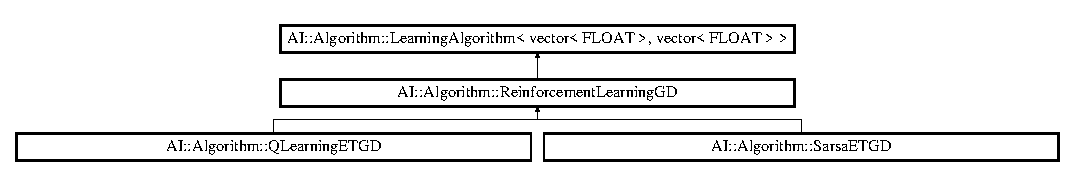
\includegraphics[height=1.931035cm]{classAI_1_1Algorithm_1_1ReinforcementLearningGD}
\end{center}
\end{figure}
\subsection*{Public Member Functions}
\begin{DoxyCompactItemize}
\item 
\hypertarget{classAI_1_1Algorithm_1_1ReinforcementLearningGD_aff76294c39401be6fbcc30970f4ccdff}{{\bfseries Reinforcement\-Learning\-G\-D} (\hyperlink{classAI_1_1Algorithm_1_1TileCode}{Tile\-Code} \&tile\-Code, A\-I\-::\-F\-L\-O\-A\-T step\-Size, A\-I\-::\-F\-L\-O\-A\-T discount\-Rate, A\-I\-::\-F\-L\-O\-A\-T lambda, \hyperlink{classAI_1_1Algorithm_1_1Policy}{Policy}$<$ vector$<$ F\-L\-O\-A\-T $>$, vector$<$ F\-L\-O\-A\-T $>$ $>$ \&policy)}\label{classAI_1_1Algorithm_1_1ReinforcementLearningGD_aff76294c39401be6fbcc30970f4ccdff}

\item 
virtual void \hyperlink{classAI_1_1Algorithm_1_1ReinforcementLearningGD_afca8d60ac090dec611f3834c0e8872c0}{update} (const \hyperlink{classAI_1_1StateAction}{State\-Action}$<$ vector$<$ F\-L\-O\-A\-T $>$, vector$<$ F\-L\-O\-A\-T $>$ $>$ \&current\-State\-Action, const vector$<$ F\-L\-O\-A\-T $>$ \&next\-State\-Vector, const F\-L\-O\-A\-T reward, const set$<$ vector$<$ F\-L\-O\-A\-T $>$ $>$ \&action\-Set)
\item 
virtual const vector$<$ F\-L\-O\-A\-T $>$ \& \hyperlink{classAI_1_1Algorithm_1_1ReinforcementLearningGD_a97a8fe122f39d0b47a9df496502c2555}{get\-Action} (const vector$<$ F\-L\-O\-A\-T $>$ \&state, const set$<$ vector$<$ F\-L\-O\-A\-T $>$ $>$ \&action\-Set)
\item 
virtual F\-L\-O\-A\-T \hyperlink{classAI_1_1Algorithm_1_1ReinforcementLearningGD_a937edc4d2b11025bccbd450163155660}{get\-State\-Action\-Value} (const \hyperlink{classAI_1_1StateAction}{State\-Action}$<$ vector$<$ F\-L\-O\-A\-T $>$, vector$<$ F\-L\-O\-A\-T $>$ $>$ \&state\-Action)
\item 
virtual void \hyperlink{classAI_1_1Algorithm_1_1ReinforcementLearningGD_ad6f2fa8bc762d6760e9c61a132ccd098}{reset} ()
\end{DoxyCompactItemize}
\subsection*{Protected Member Functions}
\begin{DoxyCompactItemize}
\item 
\hypertarget{classAI_1_1Algorithm_1_1ReinforcementLearningGD_ae03c74aee807bbf220c7e330666e3318}{F\-L\-O\-A\-T {\bfseries \-\_\-get\-State\-Action\-Value} (const \hyperlink{classAI_1_1StateAction}{State\-Action}$<$ vector$<$ F\-L\-O\-A\-T $>$, vector$<$ F\-L\-O\-A\-T $>$ $>$ \&state\-Action)}\label{classAI_1_1Algorithm_1_1ReinforcementLearningGD_ae03c74aee807bbf220c7e330666e3318}

\item 
\hypertarget{classAI_1_1Algorithm_1_1ReinforcementLearningGD_a37eb184f5219dce30af3f60f1835999e}{void {\bfseries \-\_\-build\-Action\-Values} (const set$<$ vector$<$ F\-L\-O\-A\-T $>$ $>$ \&action\-Set, const vector$<$ F\-L\-O\-A\-T $>$ \&next\-State, map$<$ action\-Vector$<$ F\-L\-O\-A\-T $>$, F\-L\-O\-A\-T $>$ \&action\-Value\-Map)}\label{classAI_1_1Algorithm_1_1ReinforcementLearningGD_a37eb184f5219dce30af3f60f1835999e}

\end{DoxyCompactItemize}
\subsection*{Protected Attributes}
\begin{DoxyCompactItemize}
\item 
\hypertarget{classAI_1_1Algorithm_1_1ReinforcementLearningGD_a881c614b3deb26f39683386a72b76dda}{\hyperlink{classAI_1_1Algorithm_1_1GradientDescent}{Gradient\-Descent} {\bfseries \-\_\-gradient\-Descent}}\label{classAI_1_1Algorithm_1_1ReinforcementLearningGD_a881c614b3deb26f39683386a72b76dda}

\end{DoxyCompactItemize}
\subsection*{Additional Inherited Members}


\subsection{Member Function Documentation}
\hypertarget{classAI_1_1Algorithm_1_1ReinforcementLearningGD_a97a8fe122f39d0b47a9df496502c2555}{\index{A\-I\-::\-Algorithm\-::\-Reinforcement\-Learning\-G\-D@{A\-I\-::\-Algorithm\-::\-Reinforcement\-Learning\-G\-D}!get\-Action@{get\-Action}}
\index{get\-Action@{get\-Action}!AI::Algorithm::ReinforcementLearningGD@{A\-I\-::\-Algorithm\-::\-Reinforcement\-Learning\-G\-D}}
\subsubsection[{get\-Action}]{\setlength{\rightskip}{0pt plus 5cm}const vector$<$ F\-L\-O\-A\-T $>$ \& A\-I\-::\-Algorithm\-::\-Reinforcement\-Learning\-G\-D\-::get\-Action (
\begin{DoxyParamCaption}
\item[{const vector$<$ F\-L\-O\-A\-T $>$ \&}]{state, }
\item[{const set$<$ vector$<$ F\-L\-O\-A\-T $>$ $>$ \&}]{action\-Set}
\end{DoxyParamCaption}
)\hspace{0.3cm}{\ttfamily [virtual]}}}\label{classAI_1_1Algorithm_1_1ReinforcementLearningGD_a97a8fe122f39d0b47a9df496502c2555}
A policy that varies between algorithms. 

Implements \hyperlink{classAI_1_1Algorithm_1_1LearningAlgorithm_afeca4eded9bc0a02312ccbbfd05f8daa}{A\-I\-::\-Algorithm\-::\-Learning\-Algorithm$<$ vector$<$ F\-L\-O\-A\-T $>$, vector$<$ F\-L\-O\-A\-T $>$ $>$}.

\hypertarget{classAI_1_1Algorithm_1_1ReinforcementLearningGD_a937edc4d2b11025bccbd450163155660}{\index{A\-I\-::\-Algorithm\-::\-Reinforcement\-Learning\-G\-D@{A\-I\-::\-Algorithm\-::\-Reinforcement\-Learning\-G\-D}!get\-State\-Action\-Value@{get\-State\-Action\-Value}}
\index{get\-State\-Action\-Value@{get\-State\-Action\-Value}!AI::Algorithm::ReinforcementLearningGD@{A\-I\-::\-Algorithm\-::\-Reinforcement\-Learning\-G\-D}}
\subsubsection[{get\-State\-Action\-Value}]{\setlength{\rightskip}{0pt plus 5cm}F\-L\-O\-A\-T A\-I\-::\-Algorithm\-::\-Reinforcement\-Learning\-G\-D\-::get\-State\-Action\-Value (
\begin{DoxyParamCaption}
\item[{const {\bf State\-Action}$<$ vector$<$ F\-L\-O\-A\-T $>$, vector$<$ F\-L\-O\-A\-T $>$ $>$ \&}]{state\-Action}
\end{DoxyParamCaption}
)\hspace{0.3cm}{\ttfamily [virtual]}}}\label{classAI_1_1Algorithm_1_1ReinforcementLearningGD_a937edc4d2b11025bccbd450163155660}
Acquire the value of the state action pair. Each algorithm group (rl, supervised, unsupervised), or specific algorithm (Q, \hyperlink{classAI_1_1Algorithm_1_1Sarsa}{Sarsa}, Gradient Descent) must implement. 
\begin{DoxyParams}{Parameters}
{\em state\-Action} & \\
\hline
\end{DoxyParams}
\begin{DoxyReturn}{Returns}
Value of state\-Action. 
\end{DoxyReturn}


Implements \hyperlink{classAI_1_1Algorithm_1_1LearningAlgorithm_a1044b2558109e8dd3d3bf5bedb9723b5}{A\-I\-::\-Algorithm\-::\-Learning\-Algorithm$<$ vector$<$ F\-L\-O\-A\-T $>$, vector$<$ F\-L\-O\-A\-T $>$ $>$}.

\hypertarget{classAI_1_1Algorithm_1_1ReinforcementLearningGD_ad6f2fa8bc762d6760e9c61a132ccd098}{\index{A\-I\-::\-Algorithm\-::\-Reinforcement\-Learning\-G\-D@{A\-I\-::\-Algorithm\-::\-Reinforcement\-Learning\-G\-D}!reset@{reset}}
\index{reset@{reset}!AI::Algorithm::ReinforcementLearningGD@{A\-I\-::\-Algorithm\-::\-Reinforcement\-Learning\-G\-D}}
\subsubsection[{reset}]{\setlength{\rightskip}{0pt plus 5cm}void A\-I\-::\-Algorithm\-::\-Reinforcement\-Learning\-G\-D\-::reset (
\begin{DoxyParamCaption}
{}
\end{DoxyParamCaption}
)\hspace{0.3cm}{\ttfamily [virtual]}}}\label{classAI_1_1Algorithm_1_1ReinforcementLearningGD_ad6f2fa8bc762d6760e9c61a132ccd098}
Reset anything prior to running episode. 

Reimplemented from \hyperlink{classAI_1_1Algorithm_1_1LearningAlgorithm_aebe650b79f39ffd46ece7adb44ddaf60}{A\-I\-::\-Algorithm\-::\-Learning\-Algorithm$<$ vector$<$ F\-L\-O\-A\-T $>$, vector$<$ F\-L\-O\-A\-T $>$ $>$}.

\hypertarget{classAI_1_1Algorithm_1_1ReinforcementLearningGD_afca8d60ac090dec611f3834c0e8872c0}{\index{A\-I\-::\-Algorithm\-::\-Reinforcement\-Learning\-G\-D@{A\-I\-::\-Algorithm\-::\-Reinforcement\-Learning\-G\-D}!update@{update}}
\index{update@{update}!AI::Algorithm::ReinforcementLearningGD@{A\-I\-::\-Algorithm\-::\-Reinforcement\-Learning\-G\-D}}
\subsubsection[{update}]{\setlength{\rightskip}{0pt plus 5cm}void A\-I\-::\-Algorithm\-::\-Reinforcement\-Learning\-G\-D\-::update (
\begin{DoxyParamCaption}
\item[{const {\bf State\-Action}$<$ vector$<$ F\-L\-O\-A\-T $>$, vector$<$ F\-L\-O\-A\-T $>$ $>$ \&}]{current\-State\-Action, }
\item[{const vector$<$ F\-L\-O\-A\-T $>$ \&}]{next\-State, }
\item[{const F\-L\-O\-A\-T}]{reward, }
\item[{const set$<$ vector$<$ F\-L\-O\-A\-T $>$ $>$ \&}]{action\-Set}
\end{DoxyParamCaption}
)\hspace{0.3cm}{\ttfamily [inline]}, {\ttfamily [virtual]}}}\label{classAI_1_1Algorithm_1_1ReinforcementLearningGD_afca8d60ac090dec611f3834c0e8872c0}
Update the state\-Action map. 
\begin{DoxyParams}{Parameters}
{\em current\-State} & \\
\hline
{\em current\-Action} & \\
\hline
{\em next\-State} & \\
\hline
{\em reward} & reward of current\-State and current\-Action. \\
\hline
{\em state\-Action} & A map of \hyperlink{classAI_1_1StateAction}{State\-Action} to Value. \\
\hline
{\em action\-Set} & A set of all actions. \\
\hline
\end{DoxyParams}
\begin{DoxyReturn}{Returns}
next action to be executed. 
\end{DoxyReturn}


Implements \hyperlink{classAI_1_1Algorithm_1_1LearningAlgorithm_a7d216d791e558e15a73083af6257ed72}{A\-I\-::\-Algorithm\-::\-Learning\-Algorithm$<$ vector$<$ F\-L\-O\-A\-T $>$, vector$<$ F\-L\-O\-A\-T $>$ $>$}.



The documentation for this class was generated from the following file\-:\begin{DoxyCompactItemize}
\item 
Algorithms/\-Supervised\-Learning/Reinforcement\-Learning\-G\-D.\-h\end{DoxyCompactItemize}

\hypertarget{classAI_1_1Algorithm_1_1Sarsa}{\section{A\-I\-:\-:Algorithm\-:\-:Sarsa$<$ S, A $>$ Class Template Reference}
\label{classAI_1_1Algorithm_1_1Sarsa}\index{A\-I\-::\-Algorithm\-::\-Sarsa$<$ S, A $>$@{A\-I\-::\-Algorithm\-::\-Sarsa$<$ S, A $>$}}
}


{\ttfamily \#include $<$Sarsa.\-h$>$}

Inheritance diagram for A\-I\-:\-:Algorithm\-:\-:Sarsa$<$ S, A $>$\-:\begin{figure}[H]
\begin{center}
\leavevmode
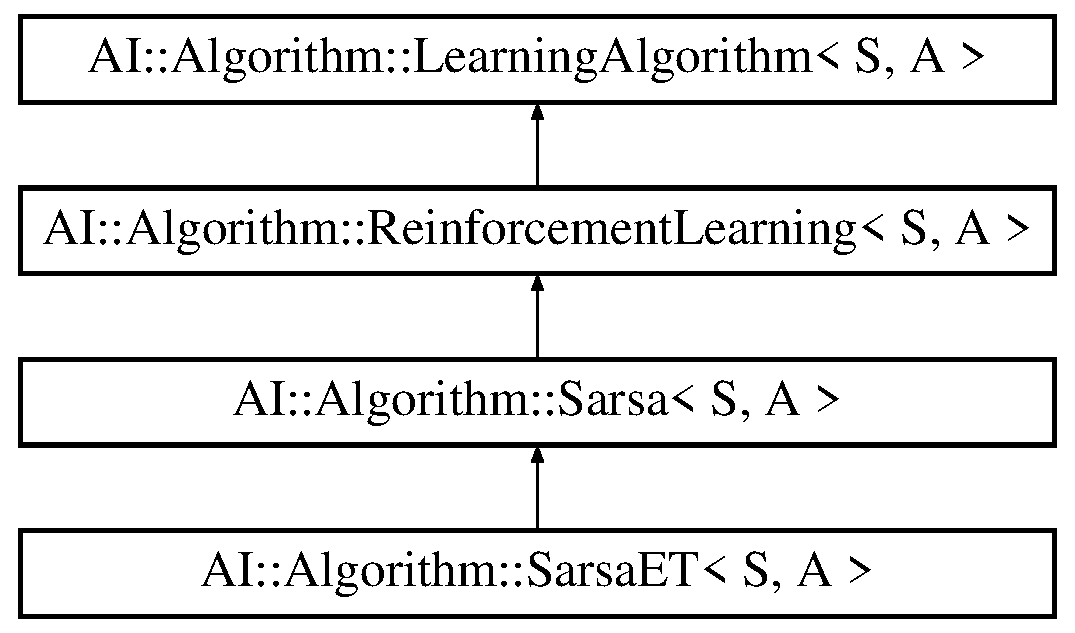
\includegraphics[height=4.000000cm]{classAI_1_1Algorithm_1_1Sarsa}
\end{center}
\end{figure}
\subsection*{Public Member Functions}
\begin{DoxyCompactItemize}
\item 
\hyperlink{classAI_1_1Algorithm_1_1Sarsa_a02dae564a53ea2284a23d047a8998fca}{Sarsa} (A\-I\-::\-F\-L\-O\-A\-T step\-Size, A\-I\-::\-F\-L\-O\-A\-T discount\-Rate, \hyperlink{classAI_1_1Algorithm_1_1Policy_1_1Policy}{Policy\-::\-Policy}$<$ S, A $>$ \&policy)
\item 
virtual void \hyperlink{classAI_1_1Algorithm_1_1Sarsa_ae1d62478d3e31cace3fb594e05f83d1c}{update} (const \hyperlink{classAI_1_1StateAction}{State\-Action}$<$ S, A $>$ \&current\-State\-Action, const S \&next\-State, const A\-I\-::\-F\-L\-O\-A\-T reward, const set$<$ A $>$ \&action\-Set)
\end{DoxyCompactItemize}
\subsection*{Additional Inherited Members}


\subsection{Detailed Description}
\subsubsection*{template$<$class S, class A$>$class A\-I\-::\-Algorithm\-::\-Sarsa$<$ S, A $>$}

\hyperlink{classAI_1_1Algorithm_1_1Sarsa}{Sarsa} 

An implementation of T\-D(0) that employs On-\/\-Policy T\-D Control. Meaning the same policy is used for approximating q$\ast$ and action-\/selection. 

\subsection{Constructor \& Destructor Documentation}
\hypertarget{classAI_1_1Algorithm_1_1Sarsa_a02dae564a53ea2284a23d047a8998fca}{\index{A\-I\-::\-Algorithm\-::\-Sarsa@{A\-I\-::\-Algorithm\-::\-Sarsa}!Sarsa@{Sarsa}}
\index{Sarsa@{Sarsa}!AI::Algorithm::Sarsa@{A\-I\-::\-Algorithm\-::\-Sarsa}}
\subsubsection[{Sarsa}]{\setlength{\rightskip}{0pt plus 5cm}template$<$class S , class A $>$ {\bf A\-I\-::\-Algorithm\-::\-Sarsa}$<$ S, A $>$\-::{\bf Sarsa} (
\begin{DoxyParamCaption}
\item[{A\-I\-::\-F\-L\-O\-A\-T}]{step\-Size, }
\item[{A\-I\-::\-F\-L\-O\-A\-T}]{discount\-Rate, }
\item[{{\bf Policy\-::\-Policy}$<$ S, A $>$ \&}]{policy}
\end{DoxyParamCaption}
)}}\label{classAI_1_1Algorithm_1_1Sarsa_a02dae564a53ea2284a23d047a8998fca}

\begin{DoxyParams}{Parameters}
{\em greedy} & determines how random is get\-Next\-State() is. A value of 1.\-0 means get\-Next\-State returns based on current likelihood of a state occuring (not random). With 0.\-0, it will not rely on the likelihood of state and return a random nextstate. \\
\hline
{\em step\-Size} & determines how the frequency is updated. A low value yields to a more accurate model of the environment but slower in learning environment. A value of 1.\-0 yields to forgeting the frequency information of all other transition states, suitable for deterministic environment. \\
\hline
\end{DoxyParams}


\subsection{Member Function Documentation}
\hypertarget{classAI_1_1Algorithm_1_1Sarsa_ae1d62478d3e31cace3fb594e05f83d1c}{\index{A\-I\-::\-Algorithm\-::\-Sarsa@{A\-I\-::\-Algorithm\-::\-Sarsa}!update@{update}}
\index{update@{update}!AI::Algorithm::Sarsa@{A\-I\-::\-Algorithm\-::\-Sarsa}}
\subsubsection[{update}]{\setlength{\rightskip}{0pt plus 5cm}template$<$class S , class A $>$ void {\bf A\-I\-::\-Algorithm\-::\-Sarsa}$<$ S, A $>$\-::update (
\begin{DoxyParamCaption}
\item[{const {\bf State\-Action}$<$ S, A $>$ \&}]{current\-State\-Action, }
\item[{const S \&}]{next\-State, }
\item[{const A\-I\-::\-F\-L\-O\-A\-T}]{reward, }
\item[{const set$<$ A $>$ \&}]{action\-Set}
\end{DoxyParamCaption}
)\hspace{0.3cm}{\ttfamily [virtual]}}}\label{classAI_1_1Algorithm_1_1Sarsa_ae1d62478d3e31cace3fb594e05f83d1c}
Update the state\-Action map. 
\begin{DoxyParams}{Parameters}
{\em current\-State} & \\
\hline
{\em current\-Action} & \\
\hline
{\em next\-State} & \\
\hline
{\em reward} & reward of the current state action value. \\
\hline
{\em action\-Set} & A set of all actions. \\
\hline
\end{DoxyParams}
\begin{DoxyReturn}{Returns}
next action to be executed. 
\end{DoxyReturn}


Reimplemented from \hyperlink{classAI_1_1Algorithm_1_1ReinforcementLearning_a25d7fa245a79e61061436dc0f1db90cb}{A\-I\-::\-Algorithm\-::\-Reinforcement\-Learning$<$ S, A $>$}.



Reimplemented in \hyperlink{classAI_1_1Algorithm_1_1SarsaET_adf13376b7ec8fdfa2b19ffadb1aa81e7}{A\-I\-::\-Algorithm\-::\-Sarsa\-E\-T$<$ S, A $>$}.



The documentation for this class was generated from the following file\-:\begin{DoxyCompactItemize}
\item 
Algorithms/\-Reinforcement\-Learning/Sarsa.\-h\end{DoxyCompactItemize}

\hypertarget{classAI_1_1Algorithm_1_1SarsaET}{\section{A\-I\-:\-:Algorithm\-:\-:Sarsa\-E\-T$<$ S, A $>$ Class Template Reference}
\label{classAI_1_1Algorithm_1_1SarsaET}\index{A\-I\-::\-Algorithm\-::\-Sarsa\-E\-T$<$ S, A $>$@{A\-I\-::\-Algorithm\-::\-Sarsa\-E\-T$<$ S, A $>$}}
}


{\ttfamily \#include $<$Sarsa\-E\-T.\-h$>$}

Inheritance diagram for A\-I\-:\-:Algorithm\-:\-:Sarsa\-E\-T$<$ S, A $>$\-:\begin{figure}[H]
\begin{center}
\leavevmode
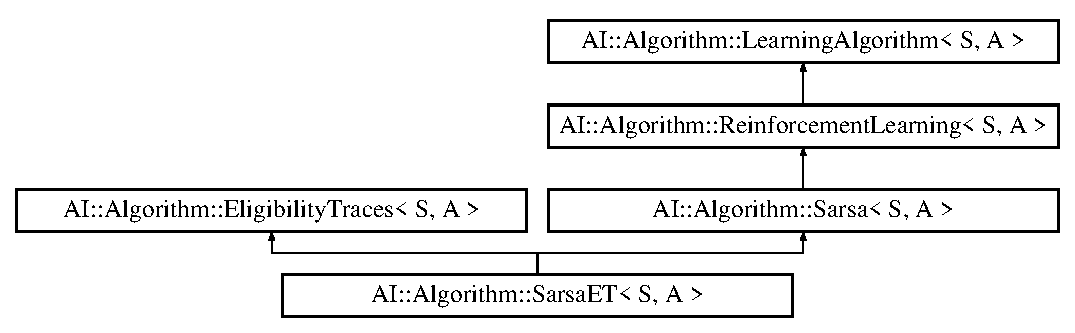
\includegraphics[height=4.000000cm]{classAI_1_1Algorithm_1_1SarsaET}
\end{center}
\end{figure}
\subsection*{Public Member Functions}
\begin{DoxyCompactItemize}
\item 
\hyperlink{classAI_1_1Algorithm_1_1SarsaET_aa934143376cc47c6e42e3ec67fb93eae}{Sarsa\-E\-T} (A\-I\-::\-F\-L\-O\-A\-T step\-Size, A\-I\-::\-F\-L\-O\-A\-T discount\-Rate, \hyperlink{classAI_1_1Algorithm_1_1Policy_1_1Policy}{Policy\-::\-Policy}$<$ S, A $>$ \&policy, A\-I\-::\-F\-L\-O\-A\-T lambda)
\item 
virtual void \hyperlink{classAI_1_1Algorithm_1_1SarsaET_adf13376b7ec8fdfa2b19ffadb1aa81e7}{update} (const \hyperlink{classAI_1_1StateAction}{State\-Action}$<$ S, A $>$ \&current\-State\-Action, const S \&next\-State, const A\-I\-::\-F\-L\-O\-A\-T reward, const set$<$ A $>$ \&action\-Set)
\end{DoxyCompactItemize}
\subsection*{Additional Inherited Members}


\subsection{Detailed Description}
\subsubsection*{template$<$class S, class A$>$class A\-I\-::\-Algorithm\-::\-Sarsa\-E\-T$<$ S, A $>$}

\hyperlink{classAI_1_1Algorithm_1_1SarsaET}{Sarsa\-E\-T} \begin{DoxySeeAlso}{See Also}
\hyperlink{classAI_1_1Algorithm_1_1Sarsa}{Sarsa} 

\hyperlink{classAI_1_1Algorithm_1_1EligibilityTraces}{Eligibility\-Traces} 
\end{DoxySeeAlso}


\subsection{Constructor \& Destructor Documentation}
\hypertarget{classAI_1_1Algorithm_1_1SarsaET_aa934143376cc47c6e42e3ec67fb93eae}{\index{A\-I\-::\-Algorithm\-::\-Sarsa\-E\-T@{A\-I\-::\-Algorithm\-::\-Sarsa\-E\-T}!Sarsa\-E\-T@{Sarsa\-E\-T}}
\index{Sarsa\-E\-T@{Sarsa\-E\-T}!AI::Algorithm::SarsaET@{A\-I\-::\-Algorithm\-::\-Sarsa\-E\-T}}
\subsubsection[{Sarsa\-E\-T}]{\setlength{\rightskip}{0pt plus 5cm}template$<$class S , class A $>$ {\bf A\-I\-::\-Algorithm\-::\-Sarsa\-E\-T}$<$ S, A $>$\-::{\bf Sarsa\-E\-T} (
\begin{DoxyParamCaption}
\item[{A\-I\-::\-F\-L\-O\-A\-T}]{step\-Size, }
\item[{A\-I\-::\-F\-L\-O\-A\-T}]{discount\-Rate, }
\item[{{\bf Policy\-::\-Policy}$<$ S, A $>$ \&}]{policy, }
\item[{A\-I\-::\-F\-L\-O\-A\-T}]{lambda}
\end{DoxyParamCaption}
)}}\label{classAI_1_1Algorithm_1_1SarsaET_aa934143376cc47c6e42e3ec67fb93eae}

\begin{DoxyParams}{Parameters}
{\em greedy} & determines how random is get\-Next\-State() is. A value of 1.\-0 means get\-Next\-State returns based on current likelihood of a state occuring (not random). With 0.\-0, it will not rely on the likelihood of state and return a random nextstate. \\
\hline
{\em step\-Size} & determines how the frequency is updated. A low value yields to a more accurate model of the environment but slower in learning environment. A value of 1.\-0 yields to forgeting the frequency information of all other transition states, suitable for deterministic environment. \\
\hline
\end{DoxyParams}


\subsection{Member Function Documentation}
\hypertarget{classAI_1_1Algorithm_1_1SarsaET_adf13376b7ec8fdfa2b19ffadb1aa81e7}{\index{A\-I\-::\-Algorithm\-::\-Sarsa\-E\-T@{A\-I\-::\-Algorithm\-::\-Sarsa\-E\-T}!update@{update}}
\index{update@{update}!AI::Algorithm::SarsaET@{A\-I\-::\-Algorithm\-::\-Sarsa\-E\-T}}
\subsubsection[{update}]{\setlength{\rightskip}{0pt plus 5cm}template$<$class S , class A $>$ void {\bf A\-I\-::\-Algorithm\-::\-Sarsa\-E\-T}$<$ S, A $>$\-::update (
\begin{DoxyParamCaption}
\item[{const {\bf State\-Action}$<$ S, A $>$ \&}]{current\-State\-Action, }
\item[{const S \&}]{next\-State, }
\item[{const A\-I\-::\-F\-L\-O\-A\-T}]{reward, }
\item[{const set$<$ A $>$ \&}]{action\-Set}
\end{DoxyParamCaption}
)\hspace{0.3cm}{\ttfamily [virtual]}}}\label{classAI_1_1Algorithm_1_1SarsaET_adf13376b7ec8fdfa2b19ffadb1aa81e7}
Update the state\-Action map. 
\begin{DoxyParams}{Parameters}
{\em current\-State} & \\
\hline
{\em current\-Action} & \\
\hline
{\em next\-State} & \\
\hline
{\em reward} & reward of the current state action value. \\
\hline
{\em state\-Action} & A map of \hyperlink{classAI_1_1StateAction}{State\-Action} to Value. \\
\hline
{\em action\-Set} & A set of all actions. \\
\hline
\end{DoxyParams}
\begin{DoxyReturn}{Returns}
next action to be executed. 
\end{DoxyReturn}


Reimplemented from \hyperlink{classAI_1_1Algorithm_1_1Sarsa_ae1d62478d3e31cace3fb594e05f83d1c}{A\-I\-::\-Algorithm\-::\-Sarsa$<$ S, A $>$}.



The documentation for this class was generated from the following file\-:\begin{DoxyCompactItemize}
\item 
Algorithms/\-Reinforcement\-Learning/Sarsa\-E\-T.\-h\end{DoxyCompactItemize}

\hypertarget{classAI_1_1Algorithm_1_1SarsaETGD}{\section{A\+I\+:\+:Algorithm\+:\+:Sarsa\+E\+T\+G\+D Class Reference}
\label{classAI_1_1Algorithm_1_1SarsaETGD}\index{A\+I\+::\+Algorithm\+::\+Sarsa\+E\+T\+G\+D@{A\+I\+::\+Algorithm\+::\+Sarsa\+E\+T\+G\+D}}
}


Gradient Descent with \hyperlink{classAI_1_1Algorithm_1_1Sarsa}{Sarsa} implementation (the same policy for learning and action selection).  




{\ttfamily \#include $<$Sarsa\+E\+T\+G\+D.\+h$>$}

Inheritance diagram for A\+I\+:\+:Algorithm\+:\+:Sarsa\+E\+T\+G\+D\+:\begin{figure}[H]
\begin{center}
\leavevmode
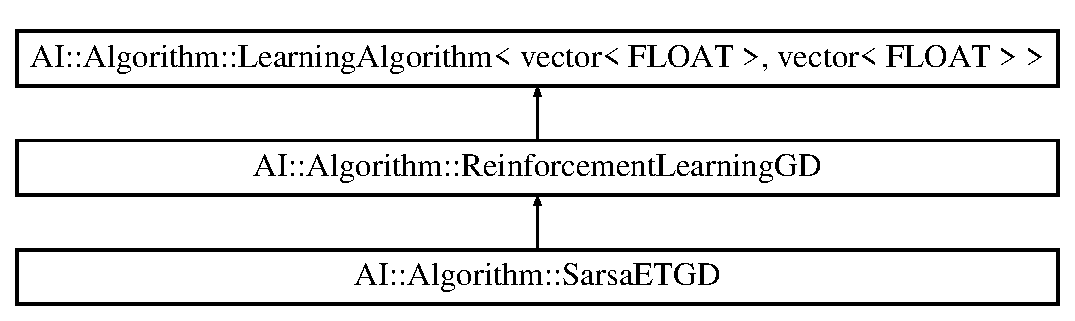
\includegraphics[height=3.000000cm]{classAI_1_1Algorithm_1_1SarsaETGD}
\end{center}
\end{figure}
\subsection*{Public Member Functions}
\begin{DoxyCompactItemize}
\item 
\hypertarget{classAI_1_1Algorithm_1_1SarsaETGD_a51da05d1ec0823c06770eaf4dc3ccdee}{{\bfseries Sarsa\+E\+T\+G\+D} (\hyperlink{classAI_1_1Algorithm_1_1TileCode}{Tile\+Code} \&tile\+Code, \hyperlink{namespaceAI_a41b74884a20833db653dded3918e05c3}{A\+I\+::\+F\+L\+O\+A\+T} step\+Size, \hyperlink{namespaceAI_a41b74884a20833db653dded3918e05c3}{A\+I\+::\+F\+L\+O\+A\+T} discount\+Rate, \hyperlink{namespaceAI_a41b74884a20833db653dded3918e05c3}{A\+I\+::\+F\+L\+O\+A\+T} lambda, \hyperlink{classAI_1_1Algorithm_1_1Policy_1_1Policy}{Policy\+::\+Policy}$<$ vector$<$ \hyperlink{namespaceAI_a41b74884a20833db653dded3918e05c3}{F\+L\+O\+A\+T} $>$, vector$<$ \hyperlink{namespaceAI_a41b74884a20833db653dded3918e05c3}{F\+L\+O\+A\+T} $>$ $>$ \&policy)}\label{classAI_1_1Algorithm_1_1SarsaETGD_a51da05d1ec0823c06770eaf4dc3ccdee}

\end{DoxyCompactItemize}
\subsection*{Additional Inherited Members}


\subsection{Detailed Description}
Gradient Descent with \hyperlink{classAI_1_1Algorithm_1_1Sarsa}{Sarsa} implementation (the same policy for learning and action selection). 

The documentation for this class was generated from the following file\+:\begin{DoxyCompactItemize}
\item 
Algorithms/\+Supervised\+Learning/Sarsa\+E\+T\+G\+D.\+h\end{DoxyCompactItemize}

\hypertarget{classAI_1_1SensorBase}{\section{A\+I\+:\+:Sensor\+Base$<$ Sensor\+Data $>$ Class Template Reference}
\label{classAI_1_1SensorBase}\index{A\+I\+::\+Sensor\+Base$<$ Sensor\+Data $>$@{A\+I\+::\+Sensor\+Base$<$ Sensor\+Data $>$}}
}


Base and interface class for all Sensor objects.  




{\ttfamily \#include $<$Sensor\+Base.\+h$>$}

Inheritance diagram for A\+I\+:\+:Sensor\+Base$<$ Sensor\+Data $>$\+:\begin{figure}[H]
\begin{center}
\leavevmode
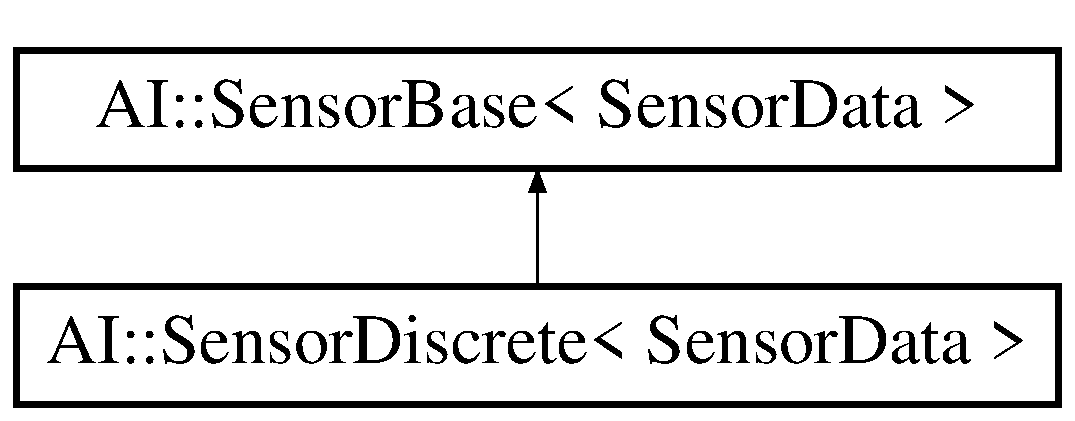
\includegraphics[height=2.000000cm]{classAI_1_1SensorBase}
\end{center}
\end{figure}
\subsection*{Public Member Functions}
\begin{DoxyCompactItemize}
\item 
virtual Sensor\+Data \hyperlink{classAI_1_1SensorBase_aad6f932417a7f8584c8a3f73ee096712}{get\+Sensor\+State} ()=0
\item 
virtual bool \hyperlink{classAI_1_1SensorBase_ad7a4098ecb3050be01d12b6c64fe0880}{is\+State} (const Sensor\+Data \&state) const =0
\item 
virtual bool \hyperlink{classAI_1_1SensorBase_acbfe2bd6f8bf57f01f4de881142cd437}{is\+Terminal\+State} (const Sensor\+Data \&state\+Data) const =0
\item 
virtual \hyperlink{namespaceAI_a41b74884a20833db653dded3918e05c3}{A\+I\+::\+F\+L\+O\+A\+T} \hyperlink{classAI_1_1SensorBase_a5f28a8bd01fc296860e2b04115d55f93}{get\+Reward} (Sensor\+Data \&sensor\+State)=0  throw (\+State\+Not\+Exist\+Exception)
\end{DoxyCompactItemize}


\subsection{Detailed Description}
\subsubsection*{template$<$class Sensor\+Data$>$class A\+I\+::\+Sensor\+Base$<$ Sensor\+Data $>$}

Base and interface class for all Sensor objects. 


\begin{DoxyTemplParams}{Template Parameters}
{\em Sensor\+Data} & State data type.\\
\hline
\end{DoxyTemplParams}
Base and interface class for all Sensor objects. For sensors with states of discrete nature, \begin{DoxySeeAlso}{See also}
\hyperlink{classAI_1_1SensorBase}{Sensor\+Base}. Otherwise, use this or \hyperlink{namespaceAI_a7ceaa7caf6e3bf156b8d2ab429d981b8}{Sensor\+Continuous}. 
\end{DoxySeeAlso}


\subsection{Member Function Documentation}
\hypertarget{classAI_1_1SensorBase_a5f28a8bd01fc296860e2b04115d55f93}{\index{A\+I\+::\+Sensor\+Base@{A\+I\+::\+Sensor\+Base}!get\+Reward@{get\+Reward}}
\index{get\+Reward@{get\+Reward}!A\+I\+::\+Sensor\+Base@{A\+I\+::\+Sensor\+Base}}
\subsubsection[{get\+Reward}]{\setlength{\rightskip}{0pt plus 5cm}template$<$class Sensor\+Data$>$ virtual {\bf A\+I\+::\+F\+L\+O\+A\+T} {\bf A\+I\+::\+Sensor\+Base}$<$ Sensor\+Data $>$\+::get\+Reward (
\begin{DoxyParamCaption}
\item[{Sensor\+Data \&}]{sensor\+State}
\end{DoxyParamCaption}
) throw  {\bf State\+Not\+Exist\+Exception}) \hspace{0.3cm}{\ttfamily [pure virtual]}}}\label{classAI_1_1SensorBase_a5f28a8bd01fc296860e2b04115d55f93}
Maps sensor\+State to its corresponding reward. 
\begin{DoxyParams}{Parameters}
{\em sensor\+State} & to be mapped to its corresponding reward. \\
\hline
\end{DoxyParams}
\begin{DoxyReturn}{Returns}
reward 
\end{DoxyReturn}
\hypertarget{classAI_1_1SensorBase_aad6f932417a7f8584c8a3f73ee096712}{\index{A\+I\+::\+Sensor\+Base@{A\+I\+::\+Sensor\+Base}!get\+Sensor\+State@{get\+Sensor\+State}}
\index{get\+Sensor\+State@{get\+Sensor\+State}!A\+I\+::\+Sensor\+Base@{A\+I\+::\+Sensor\+Base}}
\subsubsection[{get\+Sensor\+State}]{\setlength{\rightskip}{0pt plus 5cm}template$<$class Sensor\+Data$>$ virtual Sensor\+Data {\bf A\+I\+::\+Sensor\+Base}$<$ Sensor\+Data $>$\+::get\+Sensor\+State (
\begin{DoxyParamCaption}
{}
\end{DoxyParamCaption}
)\hspace{0.3cm}{\ttfamily [pure virtual]}}}\label{classAI_1_1SensorBase_aad6f932417a7f8584c8a3f73ee096712}
\begin{DoxyReturn}{Returns}
current state of agent in environment. 
\end{DoxyReturn}
\hypertarget{classAI_1_1SensorBase_ad7a4098ecb3050be01d12b6c64fe0880}{\index{A\+I\+::\+Sensor\+Base@{A\+I\+::\+Sensor\+Base}!is\+State@{is\+State}}
\index{is\+State@{is\+State}!A\+I\+::\+Sensor\+Base@{A\+I\+::\+Sensor\+Base}}
\subsubsection[{is\+State}]{\setlength{\rightskip}{0pt plus 5cm}template$<$class Sensor\+Data$>$ virtual bool {\bf A\+I\+::\+Sensor\+Base}$<$ Sensor\+Data $>$\+::is\+State (
\begin{DoxyParamCaption}
\item[{const Sensor\+Data \&}]{state}
\end{DoxyParamCaption}
) const\hspace{0.3cm}{\ttfamily [pure virtual]}}}\label{classAI_1_1SensorBase_ad7a4098ecb3050be01d12b6c64fe0880}

\begin{DoxyParams}{Parameters}
{\em state} & to determine if its in state space. \\
\hline
\end{DoxyParams}
\begin{DoxyReturn}{Returns}
true if state is domain in state space. 
\end{DoxyReturn}


Implemented in \hyperlink{classAI_1_1SensorDiscrete_a267487b20eebad42f7fcb7ee5119ac21}{A\+I\+::\+Sensor\+Discrete$<$ Sensor\+Data $>$}.

\hypertarget{classAI_1_1SensorBase_acbfe2bd6f8bf57f01f4de881142cd437}{\index{A\+I\+::\+Sensor\+Base@{A\+I\+::\+Sensor\+Base}!is\+Terminal\+State@{is\+Terminal\+State}}
\index{is\+Terminal\+State@{is\+Terminal\+State}!A\+I\+::\+Sensor\+Base@{A\+I\+::\+Sensor\+Base}}
\subsubsection[{is\+Terminal\+State}]{\setlength{\rightskip}{0pt plus 5cm}template$<$class Sensor\+Data$>$ virtual bool {\bf A\+I\+::\+Sensor\+Base}$<$ Sensor\+Data $>$\+::is\+Terminal\+State (
\begin{DoxyParamCaption}
\item[{const Sensor\+Data \&}]{state\+Data}
\end{DoxyParamCaption}
) const\hspace{0.3cm}{\ttfamily [pure virtual]}}}\label{classAI_1_1SensorBase_acbfe2bd6f8bf57f01f4de881142cd437}

\begin{DoxyParams}{Parameters}
{\em state\+Data} & to determine if it is a terminal state. \\
\hline
\end{DoxyParams}
\begin{DoxyReturn}{Returns}
true if its a terminal state. 
\end{DoxyReturn}


Implemented in \hyperlink{classAI_1_1SensorDiscrete_a1d97411a1eff0ecb1a2ee054f06bfc2c}{A\+I\+::\+Sensor\+Discrete$<$ Sensor\+Data $>$}.



The documentation for this class was generated from the following file\+:\begin{DoxyCompactItemize}
\item 
A\+I\+Base/Sensor\+Base.\+h\end{DoxyCompactItemize}

\hypertarget{classAI_1_1SensorDiscrete}{\section{A\-I\-:\-:Sensor\-Discrete$<$ Sensor\-Data $>$ Class Template Reference}
\label{classAI_1_1SensorDiscrete}\index{A\-I\-::\-Sensor\-Discrete$<$ Sensor\-Data $>$@{A\-I\-::\-Sensor\-Discrete$<$ Sensor\-Data $>$}}
}


Base class for sensors of discrete nature.  




{\ttfamily \#include $<$Sensor\-Discrete.\-h$>$}

Inheritance diagram for A\-I\-:\-:Sensor\-Discrete$<$ Sensor\-Data $>$\-:\begin{figure}[H]
\begin{center}
\leavevmode
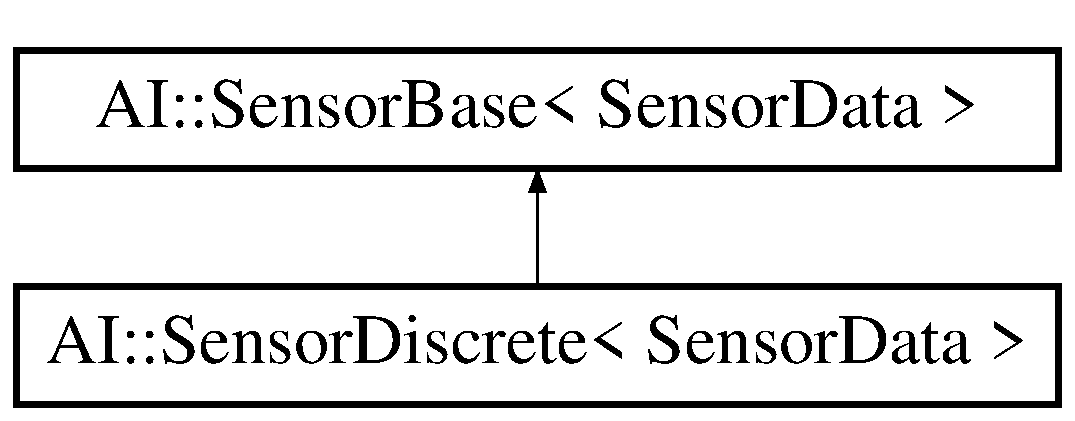
\includegraphics[height=2.000000cm]{classAI_1_1SensorDiscrete}
\end{center}
\end{figure}
\subsection*{Public Member Functions}
\begin{DoxyCompactItemize}
\item 
virtual bool \hyperlink{classAI_1_1SensorDiscrete_a267487b20eebad42f7fcb7ee5119ac21}{is\-State} (const Sensor\-Data \&state) const 
\item 
virtual bool \hyperlink{classAI_1_1SensorDiscrete_a1d97411a1eff0ecb1a2ee054f06bfc2c}{is\-Terminal\-State} (const Sensor\-Data \&state\-Data) const 
\item 
virtual const set$<$ Sensor\-Data $>$ \& \hyperlink{classAI_1_1SensorDiscrete_ab91abf49a2e0ad5592c6c0e7ac67eb5b}{get\-Observed\-States} () const 
\item 
virtual void \hyperlink{classAI_1_1SensorDiscrete_aec690a03f58beb1755b70de98df7e0a2}{add\-Terminal\-State} (const Sensor\-Data \&terminal\-Data)
\item 
virtual void \hyperlink{classAI_1_1SensorDiscrete_a9837a3640a687ea37d5f9900c3dcbcbc}{add\-Sensor\-Data} (const Sensor\-Data \&sensor\-Data)
\end{DoxyCompactItemize}


\subsection{Detailed Description}
\subsubsection*{template$<$class Sensor\-Data$>$class A\-I\-::\-Sensor\-Discrete$<$ Sensor\-Data $>$}

Base class for sensors of discrete nature. 


\begin{DoxyTemplParams}{Template Parameters}
{\em Sensor\-Data} & State data type that is discrete, e.\-g. \hyperlink{namespaceAI_ab6e14dc1e659854858a87e511f1439ec}{A\-I\-::\-U\-I\-N\-T}, \hyperlink{namespaceAI_ac74584e573f07aa4194b461b1ba7be64}{A\-I\-::\-I\-N\-T}, etc.\\
\hline
\end{DoxyTemplParams}
Base class for sensors of discrete nature. 

\subsection{Member Function Documentation}
\hypertarget{classAI_1_1SensorDiscrete_a9837a3640a687ea37d5f9900c3dcbcbc}{\index{A\-I\-::\-Sensor\-Discrete@{A\-I\-::\-Sensor\-Discrete}!add\-Sensor\-Data@{add\-Sensor\-Data}}
\index{add\-Sensor\-Data@{add\-Sensor\-Data}!AI::SensorDiscrete@{A\-I\-::\-Sensor\-Discrete}}
\subsubsection[{add\-Sensor\-Data}]{\setlength{\rightskip}{0pt plus 5cm}template$<$class Sensor\-Data $>$ void {\bf A\-I\-::\-Sensor\-Discrete}$<$ Sensor\-Data $>$\-::add\-Sensor\-Data (
\begin{DoxyParamCaption}
\item[{const Sensor\-Data \&}]{sensor\-Data}
\end{DoxyParamCaption}
)\hspace{0.3cm}{\ttfamily [virtual]}}}\label{classAI_1_1SensorDiscrete_a9837a3640a687ea37d5f9900c3dcbcbc}

\begin{DoxyParams}{Parameters}
{\em sensor\-Data} & adds a new observed sensor data. \\
\hline
\end{DoxyParams}
\hypertarget{classAI_1_1SensorDiscrete_aec690a03f58beb1755b70de98df7e0a2}{\index{A\-I\-::\-Sensor\-Discrete@{A\-I\-::\-Sensor\-Discrete}!add\-Terminal\-State@{add\-Terminal\-State}}
\index{add\-Terminal\-State@{add\-Terminal\-State}!AI::SensorDiscrete@{A\-I\-::\-Sensor\-Discrete}}
\subsubsection[{add\-Terminal\-State}]{\setlength{\rightskip}{0pt plus 5cm}template$<$class Sensor\-Data $>$ void {\bf A\-I\-::\-Sensor\-Discrete}$<$ Sensor\-Data $>$\-::add\-Terminal\-State (
\begin{DoxyParamCaption}
\item[{const Sensor\-Data \&}]{terminal\-Data}
\end{DoxyParamCaption}
)\hspace{0.3cm}{\ttfamily [virtual]}}}\label{classAI_1_1SensorDiscrete_aec690a03f58beb1755b70de98df7e0a2}

\begin{DoxyParams}{Parameters}
{\em terminal\-Data} & new terminal state to be added. \\
\hline
\end{DoxyParams}
\hypertarget{classAI_1_1SensorDiscrete_ab91abf49a2e0ad5592c6c0e7ac67eb5b}{\index{A\-I\-::\-Sensor\-Discrete@{A\-I\-::\-Sensor\-Discrete}!get\-Observed\-States@{get\-Observed\-States}}
\index{get\-Observed\-States@{get\-Observed\-States}!AI::SensorDiscrete@{A\-I\-::\-Sensor\-Discrete}}
\subsubsection[{get\-Observed\-States}]{\setlength{\rightskip}{0pt plus 5cm}template$<$class Sensor\-Data $>$ const set$<$ Sensor\-Data $>$ \& {\bf A\-I\-::\-Sensor\-Discrete}$<$ Sensor\-Data $>$\-::get\-Observed\-States (
\begin{DoxyParamCaption}
{}
\end{DoxyParamCaption}
) const\hspace{0.3cm}{\ttfamily [virtual]}}}\label{classAI_1_1SensorDiscrete_ab91abf49a2e0ad5592c6c0e7ac67eb5b}
\begin{DoxyReturn}{Returns}
set of currently observed states. 
\end{DoxyReturn}
\hypertarget{classAI_1_1SensorDiscrete_a267487b20eebad42f7fcb7ee5119ac21}{\index{A\-I\-::\-Sensor\-Discrete@{A\-I\-::\-Sensor\-Discrete}!is\-State@{is\-State}}
\index{is\-State@{is\-State}!AI::SensorDiscrete@{A\-I\-::\-Sensor\-Discrete}}
\subsubsection[{is\-State}]{\setlength{\rightskip}{0pt plus 5cm}template$<$class Sensor\-Data $>$ bool {\bf A\-I\-::\-Sensor\-Discrete}$<$ Sensor\-Data $>$\-::is\-State (
\begin{DoxyParamCaption}
\item[{const Sensor\-Data \&}]{state}
\end{DoxyParamCaption}
) const\hspace{0.3cm}{\ttfamily [virtual]}}}\label{classAI_1_1SensorDiscrete_a267487b20eebad42f7fcb7ee5119ac21}

\begin{DoxyParams}{Parameters}
{\em state} & to determine if its in state space. \\
\hline
\end{DoxyParams}
\begin{DoxyReturn}{Returns}
true if state is domain in state space. 
\end{DoxyReturn}


Implements \hyperlink{classAI_1_1SensorBase_ad7a4098ecb3050be01d12b6c64fe0880}{A\-I\-::\-Sensor\-Base$<$ Sensor\-Data $>$}.

\hypertarget{classAI_1_1SensorDiscrete_a1d97411a1eff0ecb1a2ee054f06bfc2c}{\index{A\-I\-::\-Sensor\-Discrete@{A\-I\-::\-Sensor\-Discrete}!is\-Terminal\-State@{is\-Terminal\-State}}
\index{is\-Terminal\-State@{is\-Terminal\-State}!AI::SensorDiscrete@{A\-I\-::\-Sensor\-Discrete}}
\subsubsection[{is\-Terminal\-State}]{\setlength{\rightskip}{0pt plus 5cm}template$<$class Sensor\-Data $>$ bool {\bf A\-I\-::\-Sensor\-Discrete}$<$ Sensor\-Data $>$\-::is\-Terminal\-State (
\begin{DoxyParamCaption}
\item[{const Sensor\-Data \&}]{state\-Data}
\end{DoxyParamCaption}
) const\hspace{0.3cm}{\ttfamily [virtual]}}}\label{classAI_1_1SensorDiscrete_a1d97411a1eff0ecb1a2ee054f06bfc2c}

\begin{DoxyParams}{Parameters}
{\em state\-Data} & to determine if it is a terminal state. \\
\hline
\end{DoxyParams}
\begin{DoxyReturn}{Returns}
true if its a terminal state. 
\end{DoxyReturn}


Implements \hyperlink{classAI_1_1SensorBase_acbfe2bd6f8bf57f01f4de881142cd437}{A\-I\-::\-Sensor\-Base$<$ Sensor\-Data $>$}.



The documentation for this class was generated from the following file\-:\begin{DoxyCompactItemize}
\item 
A\-I\-Base/Sensor\-Discrete.\-h\end{DoxyCompactItemize}

\hypertarget{classAI_1_1Algorithm_1_1Policy_1_1Softmax}{\section{A\-I\-:\-:Algorithm\-:\-:Policy\-:\-:Softmax$<$ S, A $>$ Class Template Reference}
\label{classAI_1_1Algorithm_1_1Policy_1_1Softmax}\index{A\-I\-::\-Algorithm\-::\-Policy\-::\-Softmax$<$ S, A $>$@{A\-I\-::\-Algorithm\-::\-Policy\-::\-Softmax$<$ S, A $>$}}
}


Greedy action is given highest selection probability, but all others are ranked and weighted according to their value estimates.  




{\ttfamily \#include $<$Softmax.\-h$>$}

Inheritance diagram for A\-I\-:\-:Algorithm\-:\-:Policy\-:\-:Softmax$<$ S, A $>$\-:\begin{figure}[H]
\begin{center}
\leavevmode
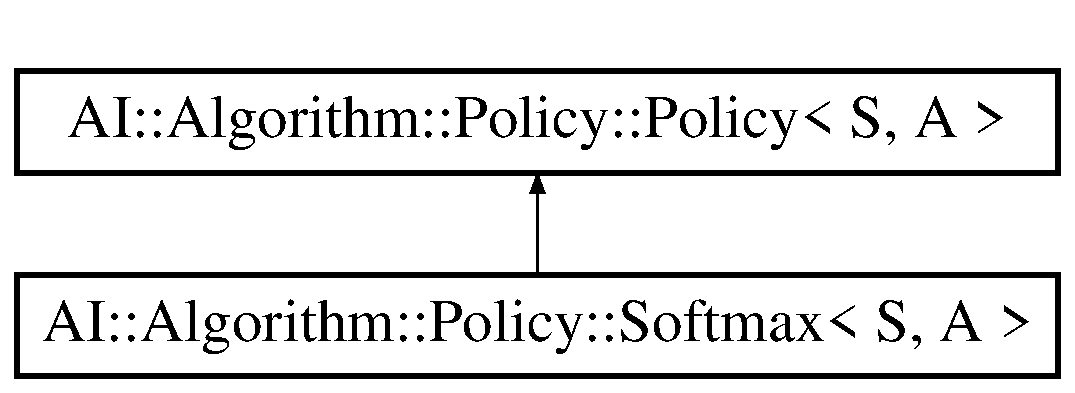
\includegraphics[height=2.000000cm]{classAI_1_1Algorithm_1_1Policy_1_1Softmax}
\end{center}
\end{figure}
\subsection*{Public Member Functions}
\begin{DoxyCompactItemize}
\item 
\hypertarget{classAI_1_1Algorithm_1_1Policy_1_1Softmax_a7f91fab0a3e3ae62fda6851f23170e9e}{{\bfseries Softmax} (\hyperlink{namespaceAI_a41b74884a20833db653dded3918e05c3}{A\-I\-::\-F\-L\-O\-A\-T} temperature)}\label{classAI_1_1Algorithm_1_1Policy_1_1Softmax_a7f91fab0a3e3ae62fda6851f23170e9e}

\item 
virtual const A \& \hyperlink{classAI_1_1Algorithm_1_1Policy_1_1Softmax_adf507bcadedab2d33e3fcc0059918d19}{get\-Action} (const map$<$ A, \hyperlink{namespaceAI_a41b74884a20833db653dded3918e05c3}{A\-I\-::\-F\-L\-O\-A\-T} $>$ \&action\-Values, const set$<$ A $>$ \&action\-Set)
\end{DoxyCompactItemize}


\subsection{Detailed Description}
\subsubsection*{template$<$class S, class A$>$class A\-I\-::\-Algorithm\-::\-Policy\-::\-Softmax$<$ S, A $>$}

Greedy action is given highest selection probability, but all others are ranked and weighted according to their value estimates. 

Greedy action is given highest selection probability, but all others are ranked and weighted according to their value estimates. In contrast with \hyperlink{classAI_1_1Algorithm_1_1Policy_1_1EpsilonGreedy}{Epsilon\-Greedy} Algorithm where non-\/greedy actions have equal chance of being chosen, non-\/greedy actions in \hyperlink{classAI_1_1Algorithm_1_1Policy_1_1Softmax}{Softmax} are chosen depending on their value estimates. The higher the value estimates, the more likely to be chosen.

In essence, \hyperlink{classAI_1_1Algorithm_1_1Policy_1_1Softmax}{Softmax} chooses action {\itshape a} with probability,

$\dfrac{e^{\frac{Q_t(a)}{\tau}}}{\sum_{i=1}^n e^{\frac{Q_t(a)}{\tau}}}$

where $\tau$ is the temperature. High temperature cause the actions to be all (nearly) equiprobable. Low temperatures cause a greater difference in selection probability that differ in their action estimates.

This policy algorithm is adapted from Sutton and Barto R\-L book 2nd edition pg 31.


\begin{DoxyTemplParams}{Template Parameters}
{\em S} & State data type. \\
\hline
{\em A} & Action data type. \\
\hline
\end{DoxyTemplParams}


\subsection{Member Function Documentation}
\hypertarget{classAI_1_1Algorithm_1_1Policy_1_1Softmax_adf507bcadedab2d33e3fcc0059918d19}{\index{A\-I\-::\-Algorithm\-::\-Policy\-::\-Softmax@{A\-I\-::\-Algorithm\-::\-Policy\-::\-Softmax}!get\-Action@{get\-Action}}
\index{get\-Action@{get\-Action}!AI::Algorithm::Policy::Softmax@{A\-I\-::\-Algorithm\-::\-Policy\-::\-Softmax}}
\subsubsection[{get\-Action}]{\setlength{\rightskip}{0pt plus 5cm}template$<$class S , class A $>$ const A \& {\bf A\-I\-::\-Algorithm\-::\-Policy\-::\-Softmax}$<$ S, A $>$\-::get\-Action (
\begin{DoxyParamCaption}
\item[{const map$<$ A, {\bf A\-I\-::\-F\-L\-O\-A\-T} $>$ \&}]{action\-Values, }
\item[{const set$<$ A $>$ \&}]{action\-Set}
\end{DoxyParamCaption}
)\hspace{0.3cm}{\ttfamily [virtual]}}}\label{classAI_1_1Algorithm_1_1Policy_1_1Softmax_adf507bcadedab2d33e3fcc0059918d19}
Returns {\bfseries action} given a mapping of actions and their value and a set of actions.


\begin{DoxyParams}{Parameters}
{\em action\-Values} & a mapping of actions to their corresponding value. \\
\hline
{\em action\-Set} & set of actions. \\
\hline
\end{DoxyParams}
\begin{DoxyReturn}{Returns}
{\bfseries action} given a mapping of actions and their value and a set of actions. 
\end{DoxyReturn}


Implements \hyperlink{classAI_1_1Algorithm_1_1Policy_1_1Policy_a1bd1f511d0f5dce4f4b080232845852c}{A\-I\-::\-Algorithm\-::\-Policy\-::\-Policy$<$ S, A $>$}.



The documentation for this class was generated from the following file\-:\begin{DoxyCompactItemize}
\item 
Algorithms/\-Policy/Softmax.\-h\end{DoxyCompactItemize}

\hypertarget{classAI_1_1StateAction}{\section{A\-I\-:\-:State\-Action$<$ S, A $>$ Class Template Reference}
\label{classAI_1_1StateAction}\index{A\-I\-::\-State\-Action$<$ S, A $>$@{A\-I\-::\-State\-Action$<$ S, A $>$}}
}


Encapsulates state action pair.  




{\ttfamily \#include $<$State\-Action.\-h$>$}

\subsection*{Public Member Functions}
\begin{DoxyCompactItemize}
\item 
\hyperlink{classAI_1_1StateAction_a0afd69cb1b7d577a1b8b51aedffc77bf}{State\-Action} ()
\item 
\hyperlink{classAI_1_1StateAction_ad2a25a219a6941a2e36b0783dd6c01cf}{State\-Action} (S state, A action)
\item 
\hypertarget{classAI_1_1StateAction_a8ba71340cc0993a198d9648ab7df8af8}{virtual bool {\bfseries operator$<$} (const \hyperlink{classAI_1_1StateAction}{State\-Action}$<$ S, A $>$ \&state\-Action) const }\label{classAI_1_1StateAction_a8ba71340cc0993a198d9648ab7df8af8}

\item 
\hypertarget{classAI_1_1StateAction_acc9bfdfd11ea817bc8b478bbd0496f96}{virtual bool {\bfseries operator$>$} (const \hyperlink{classAI_1_1StateAction}{State\-Action}$<$ S, A $>$ \&state\-Action) const }\label{classAI_1_1StateAction_acc9bfdfd11ea817bc8b478bbd0496f96}

\item 
\hypertarget{classAI_1_1StateAction_a1cddf0ba056f1be7be3f0a65d2ea7a1b}{virtual bool {\bfseries operator$<$=} (const \hyperlink{classAI_1_1StateAction}{State\-Action}$<$ S, A $>$ \&state\-Action) const }\label{classAI_1_1StateAction_a1cddf0ba056f1be7be3f0a65d2ea7a1b}

\item 
\hypertarget{classAI_1_1StateAction_a86027cd4244a8913e2b109aabe3191d4}{virtual bool {\bfseries operator$>$=} (const \hyperlink{classAI_1_1StateAction}{State\-Action}$<$ S, A $>$ \&state\-Action) const }\label{classAI_1_1StateAction_a86027cd4244a8913e2b109aabe3191d4}

\item 
\hypertarget{classAI_1_1StateAction_acb219388dc6b7a94b10ae95125b9f7b1}{virtual bool {\bfseries operator==} (const \hyperlink{classAI_1_1StateAction}{State\-Action}$<$ S, A $>$ \&state\-Action) const }\label{classAI_1_1StateAction_acb219388dc6b7a94b10ae95125b9f7b1}

\item 
\hypertarget{classAI_1_1StateAction_ad0e12e35055091f159f79a952e741f1e}{virtual bool {\bfseries operator!=} (const \hyperlink{classAI_1_1StateAction}{State\-Action}$<$ S, A $>$ \&state\-Action) const }\label{classAI_1_1StateAction_ad0e12e35055091f159f79a952e741f1e}

\item 
const S \& \hyperlink{classAI_1_1StateAction_ac9bdee11a201a7fd87071ab64b2a9743}{get\-State} () const 
\item 
const A \& \hyperlink{classAI_1_1StateAction_ae1cec3a09af9a8ca110857baa7727758}{get\-Action} () const 
\item 
void \hyperlink{classAI_1_1StateAction_a6ae04532d8d228dc4eb128c8ca223ba4}{set\-State} (const S \&state)
\item 
void \hyperlink{classAI_1_1StateAction_aa842cc33bf4d9cba87212a3a9fb94796}{set\-Action} (const A \&action)
\end{DoxyCompactItemize}
\subsection*{Protected Attributes}
\begin{DoxyCompactItemize}
\item 
\hypertarget{classAI_1_1StateAction_a0e64eecf8347c051e20e1a015ef9960a}{S \hyperlink{classAI_1_1StateAction_a0e64eecf8347c051e20e1a015ef9960a}{\-\_\-state}}\label{classAI_1_1StateAction_a0e64eecf8347c051e20e1a015ef9960a}

\begin{DoxyCompactList}\small\item\em State of state-\/action pair. \end{DoxyCompactList}\item 
\hypertarget{classAI_1_1StateAction_a951975a1853e815c68bd7400f4f1d97a}{A \hyperlink{classAI_1_1StateAction_a951975a1853e815c68bd7400f4f1d97a}{\-\_\-action}}\label{classAI_1_1StateAction_a951975a1853e815c68bd7400f4f1d97a}

\begin{DoxyCompactList}\small\item\em Action of state-\/action pair. \end{DoxyCompactList}\end{DoxyCompactItemize}


\subsection{Detailed Description}
\subsubsection*{template$<$class S, class A$>$class A\-I\-::\-State\-Action$<$ S, A $>$}

Encapsulates state action pair. 


\begin{DoxyTemplParams}{Template Parameters}
{\em S} & data type of state. \\
\hline
{\em A} & data type of action.\\
\hline
\end{DoxyTemplParams}
Encapsulates state action pair. This requires both S state and A action data type to be comparable. 

\subsection{Constructor \& Destructor Documentation}
\hypertarget{classAI_1_1StateAction_a0afd69cb1b7d577a1b8b51aedffc77bf}{\index{A\-I\-::\-State\-Action@{A\-I\-::\-State\-Action}!State\-Action@{State\-Action}}
\index{State\-Action@{State\-Action}!AI::StateAction@{A\-I\-::\-State\-Action}}
\subsubsection[{State\-Action}]{\setlength{\rightskip}{0pt plus 5cm}template$<$class S, class A$>$ {\bf A\-I\-::\-State\-Action}$<$ S, A $>$\-::{\bf State\-Action} (
\begin{DoxyParamCaption}
{}
\end{DoxyParamCaption}
)}}\label{classAI_1_1StateAction_a0afd69cb1b7d577a1b8b51aedffc77bf}
No-\/arg constructor. \hypertarget{classAI_1_1StateAction_ad2a25a219a6941a2e36b0783dd6c01cf}{\index{A\-I\-::\-State\-Action@{A\-I\-::\-State\-Action}!State\-Action@{State\-Action}}
\index{State\-Action@{State\-Action}!AI::StateAction@{A\-I\-::\-State\-Action}}
\subsubsection[{State\-Action}]{\setlength{\rightskip}{0pt plus 5cm}template$<$class S , class A $>$ {\bf A\-I\-::\-State\-Action}$<$ S, A $>$\-::{\bf State\-Action} (
\begin{DoxyParamCaption}
\item[{S}]{state, }
\item[{A}]{action}
\end{DoxyParamCaption}
)}}\label{classAI_1_1StateAction_ad2a25a219a6941a2e36b0783dd6c01cf}
Constructor for state-\/action pair. 
\begin{DoxyParams}{Parameters}
{\em state} & of state-\/action pair. \\
\hline
{\em action} & of state-\/action pair. \\
\hline
\end{DoxyParams}


\subsection{Member Function Documentation}
\hypertarget{classAI_1_1StateAction_ae1cec3a09af9a8ca110857baa7727758}{\index{A\-I\-::\-State\-Action@{A\-I\-::\-State\-Action}!get\-Action@{get\-Action}}
\index{get\-Action@{get\-Action}!AI::StateAction@{A\-I\-::\-State\-Action}}
\subsubsection[{get\-Action}]{\setlength{\rightskip}{0pt plus 5cm}template$<$class S , class A $>$ const A \& {\bf A\-I\-::\-State\-Action}$<$ S, A $>$\-::get\-Action (
\begin{DoxyParamCaption}
{}
\end{DoxyParamCaption}
) const}}\label{classAI_1_1StateAction_ae1cec3a09af9a8ca110857baa7727758}
\begin{DoxyReturn}{Returns}
return action of state-\/action pair. 
\end{DoxyReturn}
\hypertarget{classAI_1_1StateAction_ac9bdee11a201a7fd87071ab64b2a9743}{\index{A\-I\-::\-State\-Action@{A\-I\-::\-State\-Action}!get\-State@{get\-State}}
\index{get\-State@{get\-State}!AI::StateAction@{A\-I\-::\-State\-Action}}
\subsubsection[{get\-State}]{\setlength{\rightskip}{0pt plus 5cm}template$<$class S , class A $>$ const S \& {\bf A\-I\-::\-State\-Action}$<$ S, A $>$\-::get\-State (
\begin{DoxyParamCaption}
{}
\end{DoxyParamCaption}
) const}}\label{classAI_1_1StateAction_ac9bdee11a201a7fd87071ab64b2a9743}
\begin{DoxyReturn}{Returns}
return state of state-\/action pair. 
\end{DoxyReturn}
\hypertarget{classAI_1_1StateAction_aa842cc33bf4d9cba87212a3a9fb94796}{\index{A\-I\-::\-State\-Action@{A\-I\-::\-State\-Action}!set\-Action@{set\-Action}}
\index{set\-Action@{set\-Action}!AI::StateAction@{A\-I\-::\-State\-Action}}
\subsubsection[{set\-Action}]{\setlength{\rightskip}{0pt plus 5cm}template$<$class S , class A $>$ void {\bf A\-I\-::\-State\-Action}$<$ S, A $>$\-::set\-Action (
\begin{DoxyParamCaption}
\item[{const A \&}]{action}
\end{DoxyParamCaption}
)}}\label{classAI_1_1StateAction_aa842cc33bf4d9cba87212a3a9fb94796}

\begin{DoxyParams}{Parameters}
{\em action} & set the action of state-\/action pair. \\
\hline
\end{DoxyParams}
\hypertarget{classAI_1_1StateAction_a6ae04532d8d228dc4eb128c8ca223ba4}{\index{A\-I\-::\-State\-Action@{A\-I\-::\-State\-Action}!set\-State@{set\-State}}
\index{set\-State@{set\-State}!AI::StateAction@{A\-I\-::\-State\-Action}}
\subsubsection[{set\-State}]{\setlength{\rightskip}{0pt plus 5cm}template$<$class S , class A $>$ void {\bf A\-I\-::\-State\-Action}$<$ S, A $>$\-::set\-State (
\begin{DoxyParamCaption}
\item[{const S \&}]{state}
\end{DoxyParamCaption}
)}}\label{classAI_1_1StateAction_a6ae04532d8d228dc4eb128c8ca223ba4}

\begin{DoxyParams}{Parameters}
{\em state} & set the state of state-\/action pair. \\
\hline
\end{DoxyParams}


The documentation for this class was generated from the following file\-:\begin{DoxyCompactItemize}
\item 
A\-I\-Base/State\-Action.\-h\end{DoxyCompactItemize}

\hypertarget{classAI_1_1StateActionNotExistException}{\section{A\-I\-:\-:State\-Action\-Not\-Exist\-Exception Class Reference}
\label{classAI_1_1StateActionNotExistException}\index{A\-I\-::\-State\-Action\-Not\-Exist\-Exception@{A\-I\-::\-State\-Action\-Not\-Exist\-Exception}}
}


Handling situation when \hyperlink{classAI_1_1StateAction}{State\-Action} being queried does not exist.  




{\ttfamily \#include $<$State\-Action\-Not\-Exist\-Exception.\-h$>$}

Inheritance diagram for A\-I\-:\-:State\-Action\-Not\-Exist\-Exception\-:\begin{figure}[H]
\begin{center}
\leavevmode
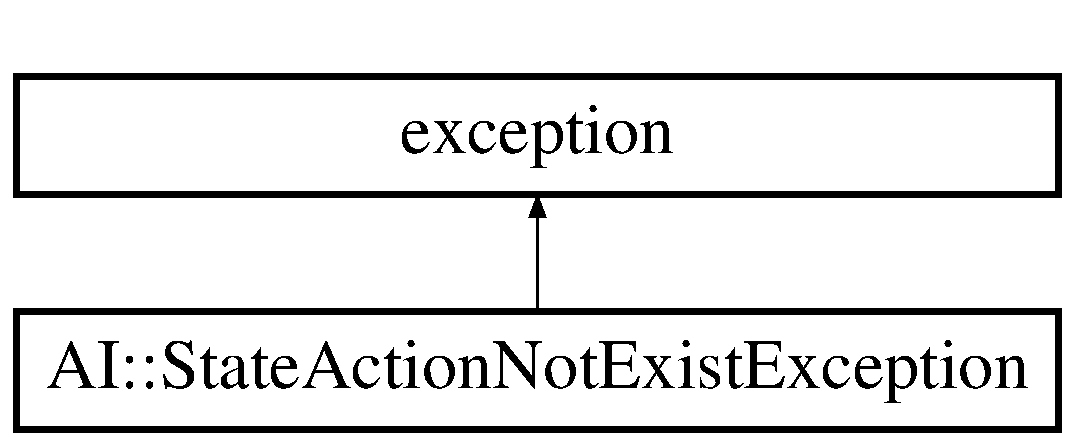
\includegraphics[height=2.000000cm]{classAI_1_1StateActionNotExistException}
\end{center}
\end{figure}
\subsection*{Public Member Functions}
\begin{DoxyCompactItemize}
\item 
\hyperlink{classAI_1_1StateActionNotExistException_abcba2ae2e7a93a728595704c3440e778}{State\-Action\-Not\-Exist\-Exception} (string extra\-Message)
\item 
\hypertarget{classAI_1_1StateActionNotExistException_a787f165434d1a3d4d9c7e5f9a3fa302a}{virtual const char $\ast$ {\bfseries what} () const   throw ()}\label{classAI_1_1StateActionNotExistException_a787f165434d1a3d4d9c7e5f9a3fa302a}

\end{DoxyCompactItemize}


\subsection{Detailed Description}
Handling situation when \hyperlink{classAI_1_1StateAction}{State\-Action} being queried does not exist. 

Handling situations when \hyperlink{classAI_1_1StateAction}{State\-Action} being query does not exist. e.\-g. map\mbox{[}\hyperlink{classAI_1_1StateAction}{State\-Action}\mbox{]} throws out of range since \hyperlink{classAI_1_1StateAction}{State\-Action} does not exist. 

\subsection{Constructor \& Destructor Documentation}
\hypertarget{classAI_1_1StateActionNotExistException_abcba2ae2e7a93a728595704c3440e778}{\index{A\-I\-::\-State\-Action\-Not\-Exist\-Exception@{A\-I\-::\-State\-Action\-Not\-Exist\-Exception}!State\-Action\-Not\-Exist\-Exception@{State\-Action\-Not\-Exist\-Exception}}
\index{State\-Action\-Not\-Exist\-Exception@{State\-Action\-Not\-Exist\-Exception}!AI::StateActionNotExistException@{A\-I\-::\-State\-Action\-Not\-Exist\-Exception}}
\subsubsection[{State\-Action\-Not\-Exist\-Exception}]{\setlength{\rightskip}{0pt plus 5cm}A\-I\-::\-State\-Action\-Not\-Exist\-Exception\-::\-State\-Action\-Not\-Exist\-Exception (
\begin{DoxyParamCaption}
\item[{string}]{extra\-Message}
\end{DoxyParamCaption}
)}}\label{classAI_1_1StateActionNotExistException_abcba2ae2e7a93a728595704c3440e778}

\begin{DoxyParams}{Parameters}
{\em extra\-Message} & To add more details of the cause of exception. This should put the exception in a better context. \\
\hline
\end{DoxyParams}


The documentation for this class was generated from the following files\-:\begin{DoxyCompactItemize}
\item 
A\-I\-Base/State\-Action\-Not\-Exist\-Exception.\-h\item 
A\-I\-Base/State\-Action\-Not\-Exist\-Exception.\-cpp\end{DoxyCompactItemize}

\hypertarget{classAI_1_1StateActionPairContainer}{\section{A\-I\-:\-:State\-Action\-Pair\-Container$<$ S, A $>$ Class Template Reference}
\label{classAI_1_1StateActionPairContainer}\index{A\-I\-::\-State\-Action\-Pair\-Container$<$ S, A $>$@{A\-I\-::\-State\-Action\-Pair\-Container$<$ S, A $>$}}
}


Encapsulates the mapping of \hyperlink{classAI_1_1StateAction}{State\-Action} to their Value.  




{\ttfamily \#include $<$State\-Action\-Pair\-Container.\-h$>$}

\subsection*{Public Member Functions}
\begin{DoxyCompactItemize}
\item 
\hyperlink{classAI_1_1StateActionPairContainer_a6b6a773f9ef9e474f879dea4de5d109b}{State\-Action\-Pair\-Container} ()
\item 
virtual void \hyperlink{classAI_1_1StateActionPairContainer_a12842518174d0af5fc89c7a86e766099}{add\-State} (const S \&state, \hyperlink{namespaceAI_a41b74884a20833db653dded3918e05c3}{A\-I\-::\-F\-L\-O\-A\-T} value, const set$<$ A $>$ \&action\-Set)
\item 
virtual void \hyperlink{classAI_1_1StateActionPairContainer_af4c9faef1c7d4e35b11f95b8a84352ae}{add\-Action} (A \&action, \hyperlink{namespaceAI_a41b74884a20833db653dded3918e05c3}{A\-I\-::\-F\-L\-O\-A\-T} value, const set$<$ S $>$ \&action\-Set)
\item 
virtual bool \hyperlink{classAI_1_1StateActionPairContainer_a4da559c1dafe0c368a331c47aede0490}{state\-In\-State\-Action\-Pair\-Map} (const S \&state, const set$<$ A $>$ \&action\-Set) const 
\item 
virtual const \hyperlink{namespaceAI_a41b74884a20833db653dded3918e05c3}{A\-I\-::\-F\-L\-O\-A\-T} \& \hyperlink{classAI_1_1StateActionPairContainer_aa3dccc9c82a2ec4130050c832e3da6c9}{get\-State\-Action\-Value} (const \hyperlink{classAI_1_1StateAction}{State\-Action}$<$ S, A $>$ \&state\-Action) const   throw (\-State\-Action\-Not\-Exist\-Exception)
\item 
virtual void \hyperlink{classAI_1_1StateActionPairContainer_a26fa5b9fd043865695e6c4adf97188d5}{set\-State\-Action\-Value} (const \hyperlink{classAI_1_1StateAction}{State\-Action}$<$ S, A $>$ \&state\-Action, \hyperlink{namespaceAI_a41b74884a20833db653dded3918e05c3}{A\-I\-::\-F\-L\-O\-A\-T} value)  throw (\-State\-Action\-Not\-Exist\-Exception)
\item 
const \hyperlink{namespaceAI_a41b74884a20833db653dded3918e05c3}{A\-I\-::\-F\-L\-O\-A\-T} \& \hyperlink{classAI_1_1StateActionPairContainer_a4dc529e9a2fa432e93fe4e4d083fce6e}{operator\mbox{[}$\,$\mbox{]}} (const \hyperlink{classAI_1_1StateAction}{State\-Action}$<$ S, A $>$ \&state\-Action) const 
\item 
map$<$ \hyperlink{classAI_1_1StateAction}{State\-Action}$<$ S, A $>$\\*
, \hyperlink{namespaceAI_a41b74884a20833db653dded3918e05c3}{A\-I\-::\-F\-L\-O\-A\-T} $>$\-::const\-\_\-iterator \hyperlink{classAI_1_1StateActionPairContainer_abb152cc2644ba6fad1da5476b746dd30}{begin} () const 
\item 
map$<$ \hyperlink{classAI_1_1StateAction}{State\-Action}$<$ S, A $>$\\*
, \hyperlink{namespaceAI_a41b74884a20833db653dded3918e05c3}{A\-I\-::\-F\-L\-O\-A\-T} $>$\-::const\-\_\-iterator \hyperlink{classAI_1_1StateActionPairContainer_a36cb0d1278cd67b4a7b4967ef6740937}{end} () const 
\end{DoxyCompactItemize}
\subsection*{Protected Attributes}
\begin{DoxyCompactItemize}
\item 
\hypertarget{classAI_1_1StateActionPairContainer_afeb95c4cb5d37ce8f8fd1a2b3518211b}{map$<$ \hyperlink{classAI_1_1StateAction}{State\-Action}$<$ S, A $>$\\*
, \hyperlink{namespaceAI_a41b74884a20833db653dded3918e05c3}{A\-I\-::\-F\-L\-O\-A\-T} $>$ \hyperlink{classAI_1_1StateActionPairContainer_afeb95c4cb5d37ce8f8fd1a2b3518211b}{\-\_\-state\-Action\-Pair\-Map}}\label{classAI_1_1StateActionPairContainer_afeb95c4cb5d37ce8f8fd1a2b3518211b}

\begin{DoxyCompactList}\small\item\em state-\/action -\/$>$ value mapping. \end{DoxyCompactList}\item 
\hypertarget{classAI_1_1StateActionPairContainer_a70b98a34845bd7744fa4e8b7c3163939}{boost\-::shared\-\_\-mutex {\bfseries \-\_\-state\-Action\-Pair\-Map\-Mutex}}\label{classAI_1_1StateActionPairContainer_a70b98a34845bd7744fa4e8b7c3163939}

\end{DoxyCompactItemize}


\subsection{Detailed Description}
\subsubsection*{template$<$class S, class A$>$class A\-I\-::\-State\-Action\-Pair\-Container$<$ S, A $>$}

Encapsulates the mapping of \hyperlink{classAI_1_1StateAction}{State\-Action} to their Value. 


\begin{DoxyTemplParams}{Template Parameters}
{\em S} & State data type. \\
\hline
{\em A} & Action data type. \\
\hline
\end{DoxyTemplParams}


\subsection{Constructor \& Destructor Documentation}
\hypertarget{classAI_1_1StateActionPairContainer_a6b6a773f9ef9e474f879dea4de5d109b}{\index{A\-I\-::\-State\-Action\-Pair\-Container@{A\-I\-::\-State\-Action\-Pair\-Container}!State\-Action\-Pair\-Container@{State\-Action\-Pair\-Container}}
\index{State\-Action\-Pair\-Container@{State\-Action\-Pair\-Container}!AI::StateActionPairContainer@{A\-I\-::\-State\-Action\-Pair\-Container}}
\subsubsection[{State\-Action\-Pair\-Container}]{\setlength{\rightskip}{0pt plus 5cm}template$<$class S , class A $>$ {\bf A\-I\-::\-State\-Action\-Pair\-Container}$<$ S, A $>$\-::{\bf State\-Action\-Pair\-Container} (
\begin{DoxyParamCaption}
{}
\end{DoxyParamCaption}
)}}\label{classAI_1_1StateActionPairContainer_a6b6a773f9ef9e474f879dea4de5d109b}
no-\/arg constructor. 

\subsection{Member Function Documentation}
\hypertarget{classAI_1_1StateActionPairContainer_af4c9faef1c7d4e35b11f95b8a84352ae}{\index{A\-I\-::\-State\-Action\-Pair\-Container@{A\-I\-::\-State\-Action\-Pair\-Container}!add\-Action@{add\-Action}}
\index{add\-Action@{add\-Action}!AI::StateActionPairContainer@{A\-I\-::\-State\-Action\-Pair\-Container}}
\subsubsection[{add\-Action}]{\setlength{\rightskip}{0pt plus 5cm}template$<$class S , class A $>$ void {\bf A\-I\-::\-State\-Action\-Pair\-Container}$<$ S, A $>$\-::add\-Action (
\begin{DoxyParamCaption}
\item[{A \&}]{action, }
\item[{{\bf A\-I\-::\-F\-L\-O\-A\-T}}]{value, }
\item[{const set$<$ S $>$ \&}]{action\-Set}
\end{DoxyParamCaption}
)\hspace{0.3cm}{\ttfamily [virtual]}}}\label{classAI_1_1StateActionPairContainer_af4c9faef1c7d4e35b11f95b8a84352ae}
Adds a new action. 
\begin{DoxyParams}{Parameters}
{\em action} & \\
\hline
{\em value} & \\
\hline
{\em action\-Set} & \\
\hline
\end{DoxyParams}
\hypertarget{classAI_1_1StateActionPairContainer_a12842518174d0af5fc89c7a86e766099}{\index{A\-I\-::\-State\-Action\-Pair\-Container@{A\-I\-::\-State\-Action\-Pair\-Container}!add\-State@{add\-State}}
\index{add\-State@{add\-State}!AI::StateActionPairContainer@{A\-I\-::\-State\-Action\-Pair\-Container}}
\subsubsection[{add\-State}]{\setlength{\rightskip}{0pt plus 5cm}template$<$class S , class A $>$ void {\bf A\-I\-::\-State\-Action\-Pair\-Container}$<$ S, A $>$\-::add\-State (
\begin{DoxyParamCaption}
\item[{const S \&}]{state, }
\item[{{\bf A\-I\-::\-F\-L\-O\-A\-T}}]{value, }
\item[{const set$<$ A $>$ \&}]{action\-Set}
\end{DoxyParamCaption}
)\hspace{0.3cm}{\ttfamily [virtual]}}}\label{classAI_1_1StateActionPairContainer_a12842518174d0af5fc89c7a86e766099}
Adds a new state. Note that in order to avoid overwriting \begin{DoxySeeAlso}{See Also}
\hyperlink{classAI_1_1StateActionPairContainer_a4da559c1dafe0c368a331c47aede0490}{state\-In\-State\-Action\-Pair\-Map()}. 
\end{DoxySeeAlso}

\begin{DoxyParams}{Parameters}
{\em state} & State to be added. \\
\hline
{\em value} & Value of the state to be added. \\
\hline
{\em action\-Array} & \\
\hline
\end{DoxyParams}
\hypertarget{classAI_1_1StateActionPairContainer_abb152cc2644ba6fad1da5476b746dd30}{\index{A\-I\-::\-State\-Action\-Pair\-Container@{A\-I\-::\-State\-Action\-Pair\-Container}!begin@{begin}}
\index{begin@{begin}!AI::StateActionPairContainer@{A\-I\-::\-State\-Action\-Pair\-Container}}
\subsubsection[{begin}]{\setlength{\rightskip}{0pt plus 5cm}template$<$class S , class A $>$ map$<$ {\bf A\-I\-::\-State\-Action}$<$ S, A $>$, {\bf A\-I\-::\-F\-L\-O\-A\-T} $>$\-::const\-\_\-iterator {\bf A\-I\-::\-State\-Action\-Pair\-Container}$<$ S, A $>$\-::begin (
\begin{DoxyParamCaption}
{}
\end{DoxyParamCaption}
) const\hspace{0.3cm}{\ttfamily [inline]}}}\label{classAI_1_1StateActionPairContainer_abb152cc2644ba6fad1da5476b746dd30}
\begin{DoxyReturn}{Returns}
begin iterator of state-\/action to value map. 
\end{DoxyReturn}
\hypertarget{classAI_1_1StateActionPairContainer_a36cb0d1278cd67b4a7b4967ef6740937}{\index{A\-I\-::\-State\-Action\-Pair\-Container@{A\-I\-::\-State\-Action\-Pair\-Container}!end@{end}}
\index{end@{end}!AI::StateActionPairContainer@{A\-I\-::\-State\-Action\-Pair\-Container}}
\subsubsection[{end}]{\setlength{\rightskip}{0pt plus 5cm}template$<$class S , class A $>$ map$<$ {\bf A\-I\-::\-State\-Action}$<$ S, A $>$, {\bf A\-I\-::\-F\-L\-O\-A\-T} $>$\-::const\-\_\-iterator {\bf A\-I\-::\-State\-Action\-Pair\-Container}$<$ S, A $>$\-::end (
\begin{DoxyParamCaption}
{}
\end{DoxyParamCaption}
) const\hspace{0.3cm}{\ttfamily [inline]}}}\label{classAI_1_1StateActionPairContainer_a36cb0d1278cd67b4a7b4967ef6740937}
\begin{DoxyReturn}{Returns}
end iterator of state-\/action to value map. 
\end{DoxyReturn}
\hypertarget{classAI_1_1StateActionPairContainer_aa3dccc9c82a2ec4130050c832e3da6c9}{\index{A\-I\-::\-State\-Action\-Pair\-Container@{A\-I\-::\-State\-Action\-Pair\-Container}!get\-State\-Action\-Value@{get\-State\-Action\-Value}}
\index{get\-State\-Action\-Value@{get\-State\-Action\-Value}!AI::StateActionPairContainer@{A\-I\-::\-State\-Action\-Pair\-Container}}
\subsubsection[{get\-State\-Action\-Value}]{\setlength{\rightskip}{0pt plus 5cm}template$<$class S , class A $>$ const {\bf A\-I\-::\-F\-L\-O\-A\-T} \& {\bf A\-I\-::\-State\-Action\-Pair\-Container}$<$ S, A $>$\-::get\-State\-Action\-Value (
\begin{DoxyParamCaption}
\item[{const {\bf State\-Action}$<$ S, A $>$ \&}]{state\-Action}
\end{DoxyParamCaption}
) const throw  {\bf State\-Action\-Not\-Exist\-Exception}) \hspace{0.3cm}{\ttfamily [inline]}, {\ttfamily [virtual]}}}\label{classAI_1_1StateActionPairContainer_aa3dccc9c82a2ec4130050c832e3da6c9}

\begin{DoxyParams}{Parameters}
{\em state\-Action} & \\
\hline
\end{DoxyParams}
\begin{DoxyReturn}{Returns}
the value of state\-Action. 
\end{DoxyReturn}

\begin{DoxyExceptions}{Exceptions}
{\em State\-Action\-Not\-Eist\-Exception} & when state\-Action does not exist. \\
\hline
\end{DoxyExceptions}
\hypertarget{classAI_1_1StateActionPairContainer_a4dc529e9a2fa432e93fe4e4d083fce6e}{\index{A\-I\-::\-State\-Action\-Pair\-Container@{A\-I\-::\-State\-Action\-Pair\-Container}!operator\mbox{[}$\,$\mbox{]}@{operator[]}}
\index{operator\mbox{[}$\,$\mbox{]}@{operator[]}!AI::StateActionPairContainer@{A\-I\-::\-State\-Action\-Pair\-Container}}
\subsubsection[{operator[]}]{\setlength{\rightskip}{0pt plus 5cm}template$<$class S , class A $>$ const {\bf A\-I\-::\-F\-L\-O\-A\-T} \& {\bf A\-I\-::\-State\-Action\-Pair\-Container}$<$ S, A $>$\-::operator\mbox{[}$\,$\mbox{]} (
\begin{DoxyParamCaption}
\item[{const {\bf State\-Action}$<$ S, A $>$ \&}]{state\-Action}
\end{DoxyParamCaption}
) const\hspace{0.3cm}{\ttfamily [inline]}}}\label{classAI_1_1StateActionPairContainer_a4dc529e9a2fa432e93fe4e4d083fce6e}
Access state-\/action value via \mbox{[}\mbox{]} operator. 
\begin{DoxyParams}{Parameters}
{\em state\-Action} & \hyperlink{classAI_1_1StateActionPairContainer}{State\-Action\-Pair\-Container}\mbox{[}state\-Action\mbox{]} \\
\hline
\end{DoxyParams}
\begin{DoxyReturn}{Returns}
\hyperlink{classAI_1_1StateActionPairContainer}{State\-Action\-Pair\-Container}\mbox{[}state\-Action\mbox{]} value. 
\end{DoxyReturn}
\hypertarget{classAI_1_1StateActionPairContainer_a26fa5b9fd043865695e6c4adf97188d5}{\index{A\-I\-::\-State\-Action\-Pair\-Container@{A\-I\-::\-State\-Action\-Pair\-Container}!set\-State\-Action\-Value@{set\-State\-Action\-Value}}
\index{set\-State\-Action\-Value@{set\-State\-Action\-Value}!AI::StateActionPairContainer@{A\-I\-::\-State\-Action\-Pair\-Container}}
\subsubsection[{set\-State\-Action\-Value}]{\setlength{\rightskip}{0pt plus 5cm}template$<$class S , class A $>$ void {\bf A\-I\-::\-State\-Action\-Pair\-Container}$<$ S, A $>$\-::set\-State\-Action\-Value (
\begin{DoxyParamCaption}
\item[{const {\bf State\-Action}$<$ S, A $>$ \&}]{state\-Action, }
\item[{{\bf A\-I\-::\-F\-L\-O\-A\-T}}]{value}
\end{DoxyParamCaption}
) throw  {\bf State\-Action\-Not\-Exist\-Exception}) \hspace{0.3cm}{\ttfamily [inline]}, {\ttfamily [virtual]}}}\label{classAI_1_1StateActionPairContainer_a26fa5b9fd043865695e6c4adf97188d5}
$ map[stateAction] \Leftarrow value $. 
\begin{DoxyParams}{Parameters}
{\em state\-Action} & to set the value of. \\
\hline
{\em value} & value of state\-Action. \\
\hline
\end{DoxyParams}

\begin{DoxyExceptions}{Exceptions}
{\em State\-Action\-No\-Exist\-Exception} & state\-Action given does not exist. \\
\hline
\end{DoxyExceptions}
\hypertarget{classAI_1_1StateActionPairContainer_a4da559c1dafe0c368a331c47aede0490}{\index{A\-I\-::\-State\-Action\-Pair\-Container@{A\-I\-::\-State\-Action\-Pair\-Container}!state\-In\-State\-Action\-Pair\-Map@{state\-In\-State\-Action\-Pair\-Map}}
\index{state\-In\-State\-Action\-Pair\-Map@{state\-In\-State\-Action\-Pair\-Map}!AI::StateActionPairContainer@{A\-I\-::\-State\-Action\-Pair\-Container}}
\subsubsection[{state\-In\-State\-Action\-Pair\-Map}]{\setlength{\rightskip}{0pt plus 5cm}template$<$class S , class A $>$ bool {\bf A\-I\-::\-State\-Action\-Pair\-Container}$<$ S, A $>$\-::state\-In\-State\-Action\-Pair\-Map (
\begin{DoxyParamCaption}
\item[{const S \&}]{state, }
\item[{const set$<$ A $>$ \&}]{action\-Set}
\end{DoxyParamCaption}
) const\hspace{0.3cm}{\ttfamily [virtual]}}}\label{classAI_1_1StateActionPairContainer_a4da559c1dafe0c368a331c47aede0490}

\begin{DoxyParams}{Parameters}
{\em state} & to be search in the \-\_\-state\-Action\-Pair\-Map. \\
\hline
\end{DoxyParams}
\begin{DoxyReturn}{Returns}
true if state is in \-\_\-state\-Action\-Pair\-Map. 
\end{DoxyReturn}


The documentation for this class was generated from the following file\-:\begin{DoxyCompactItemize}
\item 
A\-I\-Base/State\-Action\-Pair\-Container.\-h\end{DoxyCompactItemize}

\hypertarget{classAI_1_1StateActionPairValueComparison}{\section{A\-I\-:\-:State\-Action\-Pair\-Value\-Comparison$<$ S, A $>$ Class Template Reference}
\label{classAI_1_1StateActionPairValueComparison}\index{A\-I\-::\-State\-Action\-Pair\-Value\-Comparison$<$ S, A $>$@{A\-I\-::\-State\-Action\-Pair\-Value\-Comparison$<$ S, A $>$}}
}


{\ttfamily \#include $<$State\-Action\-Pair\-Value\-Comparison.\-h$>$}

\subsection*{Public Member Functions}
\begin{DoxyCompactItemize}
\item 
\hypertarget{classAI_1_1StateActionPairValueComparison_aa21d4f2cb12071606b09296288094a8e}{bool {\bfseries operator()} (const pair$<$ \hyperlink{classAI_1_1StateAction}{State\-Action}$<$ S, A $>$, A\-I\-::\-F\-L\-O\-A\-T $>$ \&lhs, const pair$<$ \hyperlink{classAI_1_1StateAction}{State\-Action}$<$ S, A $>$, A\-I\-::\-F\-L\-O\-A\-T $>$ \&rhs)}\label{classAI_1_1StateActionPairValueComparison_aa21d4f2cb12071606b09296288094a8e}

\end{DoxyCompactItemize}


\subsection{Detailed Description}
\subsubsection*{template$<$class S, class A$>$class A\-I\-::\-State\-Action\-Pair\-Value\-Comparison$<$ S, A $>$}

\hyperlink{classAI_1_1StateActionPairValueComparison}{State\-Action\-Pair\-Value\-Comparison} Created as a comparison object for State\-Action$<$\-S, A$>$ and their corresponding Value/\-Priority. This comparison object is mainly used in std\-::priority\-\_\-queue. 

The documentation for this class was generated from the following file\-:\begin{DoxyCompactItemize}
\item 
A\-I\-Base/State\-Action\-Pair\-Value\-Comparison.\-h\end{DoxyCompactItemize}

\hypertarget{classAI_1_1Algorithm_1_1StateActionTransition}{\section{A\+I\+:\+:Algorithm\+:\+:State\+Action\+Transition$<$ S $>$ Class Template Reference}
\label{classAI_1_1Algorithm_1_1StateActionTransition}\index{A\+I\+::\+Algorithm\+::\+State\+Action\+Transition$<$ S $>$@{A\+I\+::\+Algorithm\+::\+State\+Action\+Transition$<$ S $>$}}
}


Used for {\itshape modeling} environment.  




{\ttfamily \#include $<$State\+Action\+Transition.\+h$>$}

\subsection*{Public Member Functions}
\begin{DoxyCompactItemize}
\item 
\hyperlink{classAI_1_1Algorithm_1_1StateActionTransition_a0ff25726bd2c09a8d712de3fa66e541e}{State\+Action\+Transition} (const \hyperlink{namespaceAI_a41b74884a20833db653dded3918e05c3}{A\+I\+::\+F\+L\+O\+A\+T} greedy, const \hyperlink{namespaceAI_a41b74884a20833db653dded3918e05c3}{A\+I\+::\+F\+L\+O\+A\+T} step\+Size)
\item 
\hyperlink{classAI_1_1Algorithm_1_1StateActionTransition_a0b8cbca426faed815fc8389f08fe6b2c}{State\+Action\+Transition} (const \hyperlink{classAI_1_1Algorithm_1_1StateActionTransition}{State\+Action\+Transition} \&sat)
\item 
virtual void \hyperlink{classAI_1_1Algorithm_1_1StateActionTransition_a2e9b2a001f4199950f58429206a201e9}{update} (const S \&next\+State, const \hyperlink{namespaceAI_a41b74884a20833db653dded3918e05c3}{A\+I\+::\+F\+L\+O\+A\+T} reward)
\item 
virtual \hyperlink{namespaceAI_a41b74884a20833db653dded3918e05c3}{A\+I\+::\+F\+L\+O\+A\+T} \hyperlink{classAI_1_1Algorithm_1_1StateActionTransition_a73143dd7a80b3fb58ed0be0bb2962cd5}{get\+Reward} (const S \&state) const   throw (\+State\+Action\+Transition\+Exception)
\item 
virtual const S \& \hyperlink{classAI_1_1Algorithm_1_1StateActionTransition_a6f01c803796976ee877ac254a5698146}{get\+Next\+State} () const   throw (\+State\+Action\+Transition\+Exception)
\item 
size\+\_\+t \hyperlink{classAI_1_1Algorithm_1_1StateActionTransition_ae55f6b156e658e97688974ecad7cbcd1}{get\+Size} () const 
\item 
void \hyperlink{classAI_1_1Algorithm_1_1StateActionTransition_a50a3623dd0251375be981b3ac661df7d}{set\+Step\+Size} (\hyperlink{namespaceAI_a41b74884a20833db653dded3918e05c3}{A\+I\+::\+F\+L\+O\+A\+T} step\+Size)
\item 
\hyperlink{namespaceAI_a41b74884a20833db653dded3918e05c3}{A\+I\+::\+F\+L\+O\+A\+T} \hyperlink{classAI_1_1Algorithm_1_1StateActionTransition_ab0b343006fd9e43d986f4fcef9dee088}{get\+Step\+Size} () const 
\item 
void \hyperlink{classAI_1_1Algorithm_1_1StateActionTransition_af3fa54d2864692a5a55d4b9c1052349b}{set\+Greedy} (\hyperlink{namespaceAI_a41b74884a20833db653dded3918e05c3}{A\+I\+::\+F\+L\+O\+A\+T} greedy)
\item 
\hyperlink{namespaceAI_a41b74884a20833db653dded3918e05c3}{A\+I\+::\+F\+L\+O\+A\+T} \hyperlink{classAI_1_1Algorithm_1_1StateActionTransition_ad0afc4d202431930ab10c0514fd606dd}{get\+Greedy} () const 
\end{DoxyCompactItemize}


\subsection{Detailed Description}
\subsubsection*{template$<$class S$>$class A\+I\+::\+Algorithm\+::\+State\+Action\+Transition$<$ S $>$}

Used for {\itshape modeling} environment. 

This module is represents the possible transition states for some state. Every call to State\+Transition\+::update(state, reward), will increase the value of its frequency and at the same time update the reward value. Call to get\+Next\+State would then would return a state on the basis of how likely it occurs. Call to get\+Reward would return the reward of the given state. 

\subsection{Constructor \& Destructor Documentation}
\hypertarget{classAI_1_1Algorithm_1_1StateActionTransition_a0ff25726bd2c09a8d712de3fa66e541e}{\index{A\+I\+::\+Algorithm\+::\+State\+Action\+Transition@{A\+I\+::\+Algorithm\+::\+State\+Action\+Transition}!State\+Action\+Transition@{State\+Action\+Transition}}
\index{State\+Action\+Transition@{State\+Action\+Transition}!A\+I\+::\+Algorithm\+::\+State\+Action\+Transition@{A\+I\+::\+Algorithm\+::\+State\+Action\+Transition}}
\subsubsection[{State\+Action\+Transition}]{\setlength{\rightskip}{0pt plus 5cm}template$<$class S $>$ {\bf A\+I\+::\+Algorithm\+::\+State\+Action\+Transition}$<$ S $>$\+::{\bf State\+Action\+Transition} (
\begin{DoxyParamCaption}
\item[{const {\bf A\+I\+::\+F\+L\+O\+A\+T}}]{greedy, }
\item[{const {\bf A\+I\+::\+F\+L\+O\+A\+T}}]{step\+Size}
\end{DoxyParamCaption}
)}}\label{classAI_1_1Algorithm_1_1StateActionTransition_a0ff25726bd2c09a8d712de3fa66e541e}

\begin{DoxyParams}{Parameters}
{\em greedy} & determines how random is \hyperlink{classAI_1_1Algorithm_1_1StateActionTransition_a6f01c803796976ee877ac254a5698146}{get\+Next\+State()} is. A value of 1.\+0 means get\+Next\+State returns based on current likelihood of a state occuring (not random). With 0.\+0, it will not rely on the likelihood of state and return a random nextstate. \\
\hline
{\em step\+Size} & determines how the frequency is updated. A low value yields to a more accurate model of the environment but slower in learning environment. A value of 1.\+0 yields to forgeting the frequency information of all other transition states, suitable for deterministic environment. \\
\hline
\end{DoxyParams}
\hypertarget{classAI_1_1Algorithm_1_1StateActionTransition_a0b8cbca426faed815fc8389f08fe6b2c}{\index{A\+I\+::\+Algorithm\+::\+State\+Action\+Transition@{A\+I\+::\+Algorithm\+::\+State\+Action\+Transition}!State\+Action\+Transition@{State\+Action\+Transition}}
\index{State\+Action\+Transition@{State\+Action\+Transition}!A\+I\+::\+Algorithm\+::\+State\+Action\+Transition@{A\+I\+::\+Algorithm\+::\+State\+Action\+Transition}}
\subsubsection[{State\+Action\+Transition}]{\setlength{\rightskip}{0pt plus 5cm}template$<$class S $>$ {\bf A\+I\+::\+Algorithm\+::\+State\+Action\+Transition}$<$ S $>$\+::{\bf State\+Action\+Transition} (
\begin{DoxyParamCaption}
\item[{const {\bf State\+Action\+Transition}$<$ S $>$ \&}]{sat}
\end{DoxyParamCaption}
)}}\label{classAI_1_1Algorithm_1_1StateActionTransition_a0b8cbca426faed815fc8389f08fe6b2c}
Copy-\/constructor. 
\begin{DoxyParams}{Parameters}
{\em sat} & \hyperlink{classAI_1_1Algorithm_1_1StateActionTransition}{State\+Action\+Transition} to copy. \\
\hline
\end{DoxyParams}


\subsection{Member Function Documentation}
\hypertarget{classAI_1_1Algorithm_1_1StateActionTransition_ad0afc4d202431930ab10c0514fd606dd}{\index{A\+I\+::\+Algorithm\+::\+State\+Action\+Transition@{A\+I\+::\+Algorithm\+::\+State\+Action\+Transition}!get\+Greedy@{get\+Greedy}}
\index{get\+Greedy@{get\+Greedy}!A\+I\+::\+Algorithm\+::\+State\+Action\+Transition@{A\+I\+::\+Algorithm\+::\+State\+Action\+Transition}}
\subsubsection[{get\+Greedy}]{\setlength{\rightskip}{0pt plus 5cm}template$<$class S $>$ {\bf A\+I\+::\+F\+L\+O\+A\+T} {\bf A\+I\+::\+Algorithm\+::\+State\+Action\+Transition}$<$ S $>$\+::get\+Greedy (
\begin{DoxyParamCaption}
{}
\end{DoxyParamCaption}
) const}}\label{classAI_1_1Algorithm_1_1StateActionTransition_ad0afc4d202431930ab10c0514fd606dd}
\begin{DoxyReturn}{Returns}
current greediness. 
\end{DoxyReturn}
\hypertarget{classAI_1_1Algorithm_1_1StateActionTransition_a6f01c803796976ee877ac254a5698146}{\index{A\+I\+::\+Algorithm\+::\+State\+Action\+Transition@{A\+I\+::\+Algorithm\+::\+State\+Action\+Transition}!get\+Next\+State@{get\+Next\+State}}
\index{get\+Next\+State@{get\+Next\+State}!A\+I\+::\+Algorithm\+::\+State\+Action\+Transition@{A\+I\+::\+Algorithm\+::\+State\+Action\+Transition}}
\subsubsection[{get\+Next\+State}]{\setlength{\rightskip}{0pt plus 5cm}template$<$class S $>$ const S \& {\bf A\+I\+::\+Algorithm\+::\+State\+Action\+Transition}$<$ S $>$\+::get\+Next\+State (
\begin{DoxyParamCaption}
{}
\end{DoxyParamCaption}
) const throw  {\bf State\+Action\+Transition\+Exception}) \hspace{0.3cm}{\ttfamily [virtual]}}}\label{classAI_1_1Algorithm_1_1StateActionTransition_a6f01c803796976ee877ac254a5698146}
\begin{DoxyReturn}{Returns}
the possible next state based on its value. Bigger value, better chance of occuring. 
\end{DoxyReturn}

\begin{DoxyExceptions}{Exceptions}
{\em \hyperlink{classAI_1_1Algorithm_1_1StateActionTransitionException}{State\+Action\+Transition\+Exception}} & when given state don't exist. \\
\hline
\end{DoxyExceptions}
\hypertarget{classAI_1_1Algorithm_1_1StateActionTransition_a73143dd7a80b3fb58ed0be0bb2962cd5}{\index{A\+I\+::\+Algorithm\+::\+State\+Action\+Transition@{A\+I\+::\+Algorithm\+::\+State\+Action\+Transition}!get\+Reward@{get\+Reward}}
\index{get\+Reward@{get\+Reward}!A\+I\+::\+Algorithm\+::\+State\+Action\+Transition@{A\+I\+::\+Algorithm\+::\+State\+Action\+Transition}}
\subsubsection[{get\+Reward}]{\setlength{\rightskip}{0pt plus 5cm}template$<$class S $>$ {\bf A\+I\+::\+F\+L\+O\+A\+T} {\bf A\+I\+::\+Algorithm\+::\+State\+Action\+Transition}$<$ S $>$\+::get\+Reward (
\begin{DoxyParamCaption}
\item[{const S \&}]{state}
\end{DoxyParamCaption}
) const throw  {\bf State\+Action\+Transition\+Exception}) \hspace{0.3cm}{\ttfamily [virtual]}}}\label{classAI_1_1Algorithm_1_1StateActionTransition_a73143dd7a80b3fb58ed0be0bb2962cd5}
Given a state returns its latest reward info. 
\begin{DoxyParams}{Parameters}
{\em state} & to be queried of reward. \\
\hline
\end{DoxyParams}
\begin{DoxyReturn}{Returns}
reward of the state. 
\end{DoxyReturn}

\begin{DoxyExceptions}{Exceptions}
{\em \hyperlink{classAI_1_1Algorithm_1_1StateActionTransitionException}{State\+Action\+Transition\+Exception}} & when given state don't exist. \\
\hline
\end{DoxyExceptions}
\hypertarget{classAI_1_1Algorithm_1_1StateActionTransition_ae55f6b156e658e97688974ecad7cbcd1}{\index{A\+I\+::\+Algorithm\+::\+State\+Action\+Transition@{A\+I\+::\+Algorithm\+::\+State\+Action\+Transition}!get\+Size@{get\+Size}}
\index{get\+Size@{get\+Size}!A\+I\+::\+Algorithm\+::\+State\+Action\+Transition@{A\+I\+::\+Algorithm\+::\+State\+Action\+Transition}}
\subsubsection[{get\+Size}]{\setlength{\rightskip}{0pt plus 5cm}template$<$class S $>$ size\+\_\+t {\bf A\+I\+::\+Algorithm\+::\+State\+Action\+Transition}$<$ S $>$\+::get\+Size (
\begin{DoxyParamCaption}
{}
\end{DoxyParamCaption}
) const}}\label{classAI_1_1Algorithm_1_1StateActionTransition_ae55f6b156e658e97688974ecad7cbcd1}
\begin{DoxyReturn}{Returns}
the number of transition states. 
\end{DoxyReturn}
\hypertarget{classAI_1_1Algorithm_1_1StateActionTransition_ab0b343006fd9e43d986f4fcef9dee088}{\index{A\+I\+::\+Algorithm\+::\+State\+Action\+Transition@{A\+I\+::\+Algorithm\+::\+State\+Action\+Transition}!get\+Step\+Size@{get\+Step\+Size}}
\index{get\+Step\+Size@{get\+Step\+Size}!A\+I\+::\+Algorithm\+::\+State\+Action\+Transition@{A\+I\+::\+Algorithm\+::\+State\+Action\+Transition}}
\subsubsection[{get\+Step\+Size}]{\setlength{\rightskip}{0pt plus 5cm}template$<$class S $>$ {\bf A\+I\+::\+F\+L\+O\+A\+T} {\bf A\+I\+::\+Algorithm\+::\+State\+Action\+Transition}$<$ S $>$\+::get\+Step\+Size (
\begin{DoxyParamCaption}
{}
\end{DoxyParamCaption}
) const}}\label{classAI_1_1Algorithm_1_1StateActionTransition_ab0b343006fd9e43d986f4fcef9dee088}
\begin{DoxyReturn}{Returns}
current step size. 
\end{DoxyReturn}
\hypertarget{classAI_1_1Algorithm_1_1StateActionTransition_af3fa54d2864692a5a55d4b9c1052349b}{\index{A\+I\+::\+Algorithm\+::\+State\+Action\+Transition@{A\+I\+::\+Algorithm\+::\+State\+Action\+Transition}!set\+Greedy@{set\+Greedy}}
\index{set\+Greedy@{set\+Greedy}!A\+I\+::\+Algorithm\+::\+State\+Action\+Transition@{A\+I\+::\+Algorithm\+::\+State\+Action\+Transition}}
\subsubsection[{set\+Greedy}]{\setlength{\rightskip}{0pt plus 5cm}template$<$class S $>$ void {\bf A\+I\+::\+Algorithm\+::\+State\+Action\+Transition}$<$ S $>$\+::set\+Greedy (
\begin{DoxyParamCaption}
\item[{{\bf A\+I\+::\+F\+L\+O\+A\+T}}]{greedy}
\end{DoxyParamCaption}
)}}\label{classAI_1_1Algorithm_1_1StateActionTransition_af3fa54d2864692a5a55d4b9c1052349b}

\begin{DoxyParams}{Parameters}
{\em greedy} & change the greediness of the current state transition. \\
\hline
\end{DoxyParams}
\hypertarget{classAI_1_1Algorithm_1_1StateActionTransition_a50a3623dd0251375be981b3ac661df7d}{\index{A\+I\+::\+Algorithm\+::\+State\+Action\+Transition@{A\+I\+::\+Algorithm\+::\+State\+Action\+Transition}!set\+Step\+Size@{set\+Step\+Size}}
\index{set\+Step\+Size@{set\+Step\+Size}!A\+I\+::\+Algorithm\+::\+State\+Action\+Transition@{A\+I\+::\+Algorithm\+::\+State\+Action\+Transition}}
\subsubsection[{set\+Step\+Size}]{\setlength{\rightskip}{0pt plus 5cm}template$<$class S $>$ void {\bf A\+I\+::\+Algorithm\+::\+State\+Action\+Transition}$<$ S $>$\+::set\+Step\+Size (
\begin{DoxyParamCaption}
\item[{{\bf A\+I\+::\+F\+L\+O\+A\+T}}]{step\+Size}
\end{DoxyParamCaption}
)}}\label{classAI_1_1Algorithm_1_1StateActionTransition_a50a3623dd0251375be981b3ac661df7d}

\begin{DoxyParams}{Parameters}
{\em step\+Size} & change the current step size. \\
\hline
\end{DoxyParams}
\hypertarget{classAI_1_1Algorithm_1_1StateActionTransition_a2e9b2a001f4199950f58429206a201e9}{\index{A\+I\+::\+Algorithm\+::\+State\+Action\+Transition@{A\+I\+::\+Algorithm\+::\+State\+Action\+Transition}!update@{update}}
\index{update@{update}!A\+I\+::\+Algorithm\+::\+State\+Action\+Transition@{A\+I\+::\+Algorithm\+::\+State\+Action\+Transition}}
\subsubsection[{update}]{\setlength{\rightskip}{0pt plus 5cm}template$<$class S $>$ void {\bf A\+I\+::\+Algorithm\+::\+State\+Action\+Transition}$<$ S $>$\+::update (
\begin{DoxyParamCaption}
\item[{const S \&}]{next\+State, }
\item[{const {\bf A\+I\+::\+F\+L\+O\+A\+T}}]{reward}
\end{DoxyParamCaption}
)\hspace{0.3cm}{\ttfamily [virtual]}}}\label{classAI_1_1Algorithm_1_1StateActionTransition_a2e9b2a001f4199950f58429206a201e9}
By adding a new state, this updates the information of all other states. Frequency of all state, not next\+State will decrease and frequency of next\+State will increase. The reward will update the value of the next\+State. 
\begin{DoxyParams}{Parameters}
{\em next\+State} & to be added or increased frequency value and update reward value. \\
\hline
{\em reward} & to update the value of the next\+State. \\
\hline
\end{DoxyParams}


The documentation for this class was generated from the following file\+:\begin{DoxyCompactItemize}
\item 
Algorithms/\+Reinforcement\+Learning/State\+Action\+Transition.\+h\end{DoxyCompactItemize}

\hypertarget{classAI_1_1Algorithm_1_1StateActionTransitionException}{\section{A\+I\+:\+:Algorithm\+:\+:State\+Action\+Transition\+Exception Class Reference}
\label{classAI_1_1Algorithm_1_1StateActionTransitionException}\index{A\+I\+::\+Algorithm\+::\+State\+Action\+Transition\+Exception@{A\+I\+::\+Algorithm\+::\+State\+Action\+Transition\+Exception}}
}


exception when \hyperlink{classAI_1_1Algorithm_1_1StateActionTransition}{State\+Action\+Transition} does not exist.  




{\ttfamily \#include $<$State\+Action\+Transition\+Exception.\+h$>$}

Inheritance diagram for A\+I\+:\+:Algorithm\+:\+:State\+Action\+Transition\+Exception\+:\begin{figure}[H]
\begin{center}
\leavevmode
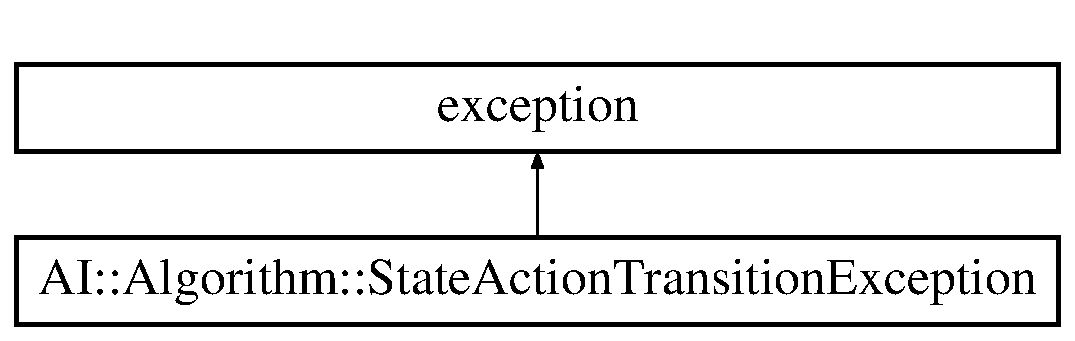
\includegraphics[height=2.000000cm]{classAI_1_1Algorithm_1_1StateActionTransitionException}
\end{center}
\end{figure}
\subsection*{Public Member Functions}
\begin{DoxyCompactItemize}
\item 
\hypertarget{classAI_1_1Algorithm_1_1StateActionTransitionException_a7b8bf70b19728f4b6616ae726c88fc54}{{\bfseries State\+Action\+Transition\+Exception} (std\+::string extra\+Msg)}\label{classAI_1_1Algorithm_1_1StateActionTransitionException_a7b8bf70b19728f4b6616ae726c88fc54}

\item 
\hypertarget{classAI_1_1Algorithm_1_1StateActionTransitionException_a3af53ac148abbcfd435a8da87cc92e29}{virtual const char $\ast$ {\bfseries what} () const   throw ()}\label{classAI_1_1Algorithm_1_1StateActionTransitionException_a3af53ac148abbcfd435a8da87cc92e29}

\end{DoxyCompactItemize}


\subsection{Detailed Description}
exception when \hyperlink{classAI_1_1Algorithm_1_1StateActionTransition}{State\+Action\+Transition} does not exist. 

The documentation for this class was generated from the following files\+:\begin{DoxyCompactItemize}
\item 
Algorithms/\+Reinforcement\+Learning/State\+Action\+Transition\+Exception.\+h\item 
Algorithms/\+Reinforcement\+Learning/State\+Action\+Transition\+Exception.\+cpp\end{DoxyCompactItemize}

\hypertarget{classAI_1_1StateNotExistException}{\section{A\+I\+:\+:State\+Not\+Exist\+Exception Class Reference}
\label{classAI_1_1StateNotExistException}\index{A\+I\+::\+State\+Not\+Exist\+Exception@{A\+I\+::\+State\+Not\+Exist\+Exception}}
}


exception when State does not exist.  




{\ttfamily \#include $<$State\+Not\+Exist\+Exception.\+h$>$}

Inheritance diagram for A\+I\+:\+:State\+Not\+Exist\+Exception\+:\begin{figure}[H]
\begin{center}
\leavevmode
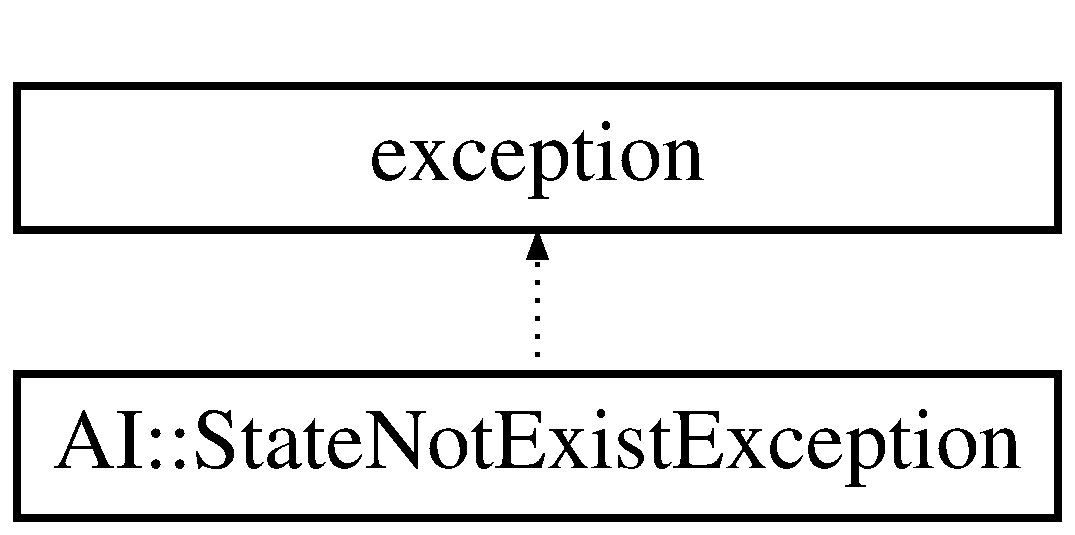
\includegraphics[height=2.000000cm]{classAI_1_1StateNotExistException}
\end{center}
\end{figure}
\subsection*{Public Member Functions}
\begin{DoxyCompactItemize}
\item 
\hypertarget{classAI_1_1StateNotExistException_afba608702bcd8aeb728c3a6a1ff109c1}{{\bfseries State\+Not\+Exist\+Exception} (string extra\+Message)}\label{classAI_1_1StateNotExistException_afba608702bcd8aeb728c3a6a1ff109c1}

\item 
\hypertarget{classAI_1_1StateNotExistException_a97f180bdeef94eb9939bb80caa008951}{virtual const char $\ast$ {\bfseries what} () const   throw ()}\label{classAI_1_1StateNotExistException_a97f180bdeef94eb9939bb80caa008951}

\end{DoxyCompactItemize}


\subsection{Detailed Description}
exception when State does not exist. 



The documentation for this class was generated from the following files\+:\begin{DoxyCompactItemize}
\item 
A\+I\+Base/State\+Not\+Exist\+Exception.\+h\item 
A\+I\+Base/State\+Not\+Exist\+Exception.\+cpp\end{DoxyCompactItemize}

\hypertarget{classAI_1_1Algorithm_1_1Hash_1_1SuperFastHash}{\section{A\+I\+:\+:Algorithm\+:\+:Hash\+:\+:Super\+Fast\+Hash Class Reference}
\label{classAI_1_1Algorithm_1_1Hash_1_1SuperFastHash}\index{A\+I\+::\+Algorithm\+::\+Hash\+::\+Super\+Fast\+Hash@{A\+I\+::\+Algorithm\+::\+Hash\+::\+Super\+Fast\+Hash}}
}


\hyperlink{classAI_1_1Algorithm_1_1Hash_1_1SuperFastHash}{Super\+Fast\+Hash} implementation encapsulated.  




{\ttfamily \#include $<$Hash\+Super\+Fast\+Hash.\+h$>$}

Inheritance diagram for A\+I\+:\+:Algorithm\+:\+:Hash\+:\+:Super\+Fast\+Hash\+:\begin{figure}[H]
\begin{center}
\leavevmode
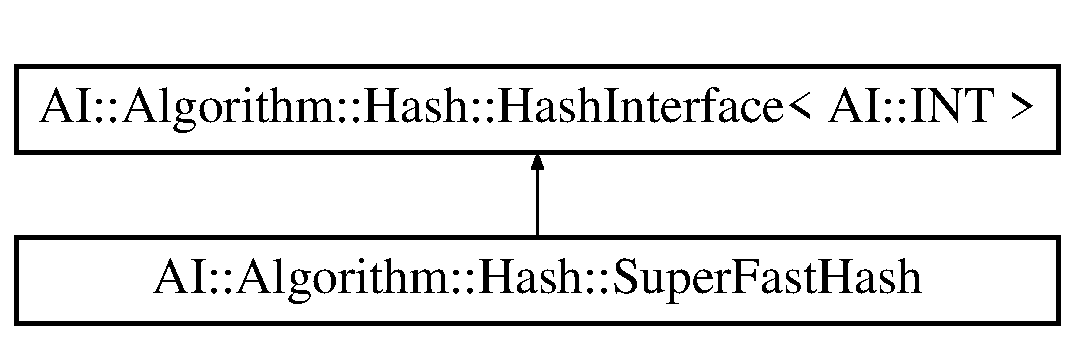
\includegraphics[height=2.000000cm]{classAI_1_1Algorithm_1_1Hash_1_1SuperFastHash}
\end{center}
\end{figure}
\subsection*{Public Member Functions}
\begin{DoxyCompactItemize}
\item 
virtual \hyperlink{namespaceAI_ac74584e573f07aa4194b461b1ba7be64}{A\+I\+::\+I\+N\+T} \hyperlink{classAI_1_1Algorithm_1_1Hash_1_1SuperFastHash_a242ccb7975bd45b30a945d9649170629}{hash} (const \hyperlink{namespaceAI_a9d4bcda82fe0f9aac3c4861e24491581}{A\+I\+::\+B\+Y\+T\+E} $\ast$const byte\+Array, size\+\_\+t len)
\item 
\hypertarget{classAI_1_1Algorithm_1_1Hash_1_1SuperFastHash_a08a5db31d857cc7706529d185827586a}{virtual \hyperlink{namespaceAI_ac74584e573f07aa4194b461b1ba7be64}{A\+I\+::\+I\+N\+T} {\bfseries hash} (const vector$<$ \hyperlink{namespaceAI_a9d4bcda82fe0f9aac3c4861e24491581}{A\+I\+::\+B\+Y\+T\+E} $>$ \&byte\+Array)}\label{classAI_1_1Algorithm_1_1Hash_1_1SuperFastHash_a08a5db31d857cc7706529d185827586a}

\end{DoxyCompactItemize}


\subsection{Detailed Description}
\hyperlink{classAI_1_1Algorithm_1_1Hash_1_1SuperFastHash}{Super\+Fast\+Hash} implementation encapsulated. 

\subsection{Member Function Documentation}
\hypertarget{classAI_1_1Algorithm_1_1Hash_1_1SuperFastHash_a242ccb7975bd45b30a945d9649170629}{\index{A\+I\+::\+Algorithm\+::\+Hash\+::\+Super\+Fast\+Hash@{A\+I\+::\+Algorithm\+::\+Hash\+::\+Super\+Fast\+Hash}!hash@{hash}}
\index{hash@{hash}!A\+I\+::\+Algorithm\+::\+Hash\+::\+Super\+Fast\+Hash@{A\+I\+::\+Algorithm\+::\+Hash\+::\+Super\+Fast\+Hash}}
\subsubsection[{hash}]{\setlength{\rightskip}{0pt plus 5cm}{\bf A\+I\+::\+I\+N\+T} A\+I\+::\+Algorithm\+::\+Hash\+::\+Super\+Fast\+Hash\+::hash (
\begin{DoxyParamCaption}
\item[{const {\bf A\+I\+::\+B\+Y\+T\+E} $\ast$const}]{byte\+Array, }
\item[{size\+\_\+t}]{len}
\end{DoxyParamCaption}
)\hspace{0.3cm}{\ttfamily [virtual]}}}\label{classAI_1_1Algorithm_1_1Hash_1_1SuperFastHash_a242ccb7975bd45b30a945d9649170629}

\begin{DoxyParams}{Parameters}
{\em byte\+Array} & \\
\hline
{\em len} & \\
\hline
\end{DoxyParams}
\begin{DoxyReturn}{Returns}
h(byte\+Array) 
\end{DoxyReturn}


Implements \hyperlink{classAI_1_1Algorithm_1_1Hash_1_1HashInterface_ae31d650fd044e3ef372cae18a422e0d9}{A\+I\+::\+Algorithm\+::\+Hash\+::\+Hash\+Interface$<$ A\+I\+::\+I\+N\+T $>$}.



The documentation for this class was generated from the following files\+:\begin{DoxyCompactItemize}
\item 
Algorithms/\+Hash/Hash\+Super\+Fast\+Hash.\+h\item 
Algorithms/\+Hash/Hash\+Super\+Fast\+Hash.\+cpp\end{DoxyCompactItemize}

\hypertarget{classAI_1_1Algorithm_1_1TileCode}{\section{A\+I\+:\+:Algorithm\+:\+:Tile\+Code Class Reference}
\label{classAI_1_1Algorithm_1_1TileCode}\index{A\+I\+::\+Algorithm\+::\+Tile\+Code@{A\+I\+::\+Algorithm\+::\+Tile\+Code}}
}


Base object encapsulate tile coding.  




{\ttfamily \#include $<$Tile\+Code.\+h$>$}

Inheritance diagram for A\+I\+:\+:Algorithm\+:\+:Tile\+Code\+:\begin{figure}[H]
\begin{center}
\leavevmode
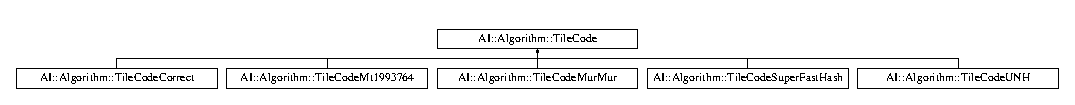
\includegraphics[height=0.957265cm]{classAI_1_1Algorithm_1_1TileCode}
\end{center}
\end{figure}
\subsection*{Public Member Functions}
\begin{DoxyCompactItemize}
\item 
\hyperlink{classAI_1_1Algorithm_1_1TileCode_a5c143dc170aca9699e68c808d91f1ffe}{Tile\+Code} (vector$<$ \hyperlink{classAI_1_1Algorithm_1_1DimensionInfo}{Dimension\+Info}$<$ \hyperlink{namespaceAI_a41b74884a20833db653dded3918e05c3}{F\+L\+O\+A\+T} $>$ $>$ dimensional\+Infos, size\+\_\+t num\+Tilings)
\item 
virtual void \hyperlink{classAI_1_1Algorithm_1_1TileCode_ad2ba639c550e7d267d066e54b20f6000}{get\+Feature\+Vector} (const \hyperlink{namespaceAI_aff63ec21d97dd5f086fddbc3103f5707}{S\+T\+A\+T\+E\+\_\+\+C\+O\+N\+T} \&parameters, \hyperlink{namespaceAI_a23a39e1b301a5c1345fa508796940631}{F\+E\+A\+T\+U\+R\+E\+\_\+\+V\+E\+C\+T\+O\+R} \&fv)=0
\item 
size\+\_\+t \hyperlink{classAI_1_1Algorithm_1_1TileCode_a3d757b2d7e6cf273c54f007230b69406}{get\+Size} () const 
\item 
void \hyperlink{classAI_1_1Algorithm_1_1TileCode_aad4bf93d21b47fe00c8e64957157dca1}{set\+Num\+Tilings} (size\+\_\+t num\+Tilings)
\item 
size\+\_\+t \hyperlink{classAI_1_1Algorithm_1_1TileCode_a540d24d750bf47835ed950b4ef54486a}{get\+Num\+Tilings} () const 
\item 
size\+\_\+t \hyperlink{classAI_1_1Algorithm_1_1TileCode_aa80f909ef2bf2039c4ea7b468bf796a5}{get\+Dimension} () const 
\end{DoxyCompactItemize}
\subsection*{Protected Member Functions}
\begin{DoxyCompactItemize}
\item 
size\+\_\+t \hyperlink{classAI_1_1Algorithm_1_1TileCode_a918fe826ad83e42c65bce7abfa35ad58}{\+\_\+calculate\+Size\+Cache} ()
\item 
size\+\_\+t \hyperlink{classAI_1_1Algorithm_1_1TileCode_a89e1188441fe9f07b4f9fa6394003a89}{\+\_\+param\+To\+Grid\+Value} (\hyperlink{namespaceAI_a41b74884a20833db653dded3918e05c3}{A\+I\+::\+F\+L\+O\+A\+T} param, size\+\_\+t tiling\+Index, size\+\_\+t dimension\+Index)
\end{DoxyCompactItemize}
\subsection*{Protected Attributes}
\begin{DoxyCompactItemize}
\item 
\hypertarget{classAI_1_1Algorithm_1_1TileCode_a3f5b849919d62c2167d28e06efcadb3b}{size\+\_\+t \hyperlink{classAI_1_1Algorithm_1_1TileCode_a3f5b849919d62c2167d28e06efcadb3b}{\+\_\+dimension}}\label{classAI_1_1Algorithm_1_1TileCode_a3f5b849919d62c2167d28e06efcadb3b}

\begin{DoxyCompactList}\small\item\em How many dimension. \end{DoxyCompactList}\item 
\hypertarget{classAI_1_1Algorithm_1_1TileCode_ae45e259692f779b3d6881e74a3c944c5}{size\+\_\+t \hyperlink{classAI_1_1Algorithm_1_1TileCode_ae45e259692f779b3d6881e74a3c944c5}{\+\_\+num\+Tilings}}\label{classAI_1_1Algorithm_1_1TileCode_ae45e259692f779b3d6881e74a3c944c5}

\begin{DoxyCompactList}\small\item\em How many tilings/also known as sample. \end{DoxyCompactList}\item 
\hypertarget{classAI_1_1Algorithm_1_1TileCode_af55344828d37574d90f9bb0ed939cdba}{vector$<$ \hyperlink{classAI_1_1Algorithm_1_1DimensionInfo}{Dimension\+Info}$<$ \hyperlink{namespaceAI_a41b74884a20833db653dded3918e05c3}{F\+L\+O\+A\+T} $>$ $>$ \hyperlink{classAI_1_1Algorithm_1_1TileCode_af55344828d37574d90f9bb0ed939cdba}{\+\_\+dimensional\+Infos}}\label{classAI_1_1Algorithm_1_1TileCode_af55344828d37574d90f9bb0ed939cdba}

\begin{DoxyCompactList}\small\item\em Contains information for each dimension. \end{DoxyCompactList}\item 
\hypertarget{classAI_1_1Algorithm_1_1TileCode_a8b690cd8628f8772856ab914d8469f03}{std\+::random\+\_\+device {\bfseries \+\_\+random\+Device}}\label{classAI_1_1Algorithm_1_1TileCode_a8b690cd8628f8772856ab914d8469f03}

\item 
\hypertarget{classAI_1_1Algorithm_1_1TileCode_ae0ac4ab46768a4c60c0470851b974d92}{std\+::default\+\_\+random\+\_\+engine {\bfseries \+\_\+pseudo\+R\+N\+G}}\label{classAI_1_1Algorithm_1_1TileCode_ae0ac4ab46768a4c60c0470851b974d92}

\item 
size\+\_\+t \hyperlink{classAI_1_1Algorithm_1_1TileCode_a233a9e2d90544b8070788bb65b6bde52}{\+\_\+size\+Cache}
\item 
vector$<$ vector$<$ \hyperlink{namespaceAI_a41b74884a20833db653dded3918e05c3}{A\+I\+::\+F\+L\+O\+A\+T} $>$ $>$ \hyperlink{classAI_1_1Algorithm_1_1TileCode_afbe28b5932dec68724048dbccfd9a338}{\+\_\+random\+Offsets}
\end{DoxyCompactItemize}


\subsection{Detailed Description}
Base object encapsulate tile coding. 

For an in-\/dept explaination of Tile Coding, see \href{tileCoding.html}{\tt Tile Coding} 

\subsection{Constructor \& Destructor Documentation}
\hypertarget{classAI_1_1Algorithm_1_1TileCode_a5c143dc170aca9699e68c808d91f1ffe}{\index{A\+I\+::\+Algorithm\+::\+Tile\+Code@{A\+I\+::\+Algorithm\+::\+Tile\+Code}!Tile\+Code@{Tile\+Code}}
\index{Tile\+Code@{Tile\+Code}!A\+I\+::\+Algorithm\+::\+Tile\+Code@{A\+I\+::\+Algorithm\+::\+Tile\+Code}}
\subsubsection[{Tile\+Code}]{\setlength{\rightskip}{0pt plus 5cm}A\+I\+::\+Algorithm\+::\+Tile\+Code\+::\+Tile\+Code (
\begin{DoxyParamCaption}
\item[{vector$<$ {\bf Dimension\+Info}$<$ {\bf F\+L\+O\+A\+T} $>$ $>$}]{dimensional\+Infos, }
\item[{size\+\_\+t}]{num\+Tilings}
\end{DoxyParamCaption}
)}}\label{classAI_1_1Algorithm_1_1TileCode_a5c143dc170aca9699e68c808d91f1ffe}

\begin{DoxyParams}{Parameters}
{\em dimensional\+Infos} & A vector dimensional\+Infos. \\
\hline
{\em num\+Tilings} & The higher the value, the more accurate is the generalization. \\
\hline
\end{DoxyParams}


\subsection{Member Function Documentation}
\hypertarget{classAI_1_1Algorithm_1_1TileCode_a918fe826ad83e42c65bce7abfa35ad58}{\index{A\+I\+::\+Algorithm\+::\+Tile\+Code@{A\+I\+::\+Algorithm\+::\+Tile\+Code}!\+\_\+calculate\+Size\+Cache@{\+\_\+calculate\+Size\+Cache}}
\index{\+\_\+calculate\+Size\+Cache@{\+\_\+calculate\+Size\+Cache}!A\+I\+::\+Algorithm\+::\+Tile\+Code@{A\+I\+::\+Algorithm\+::\+Tile\+Code}}
\subsubsection[{\+\_\+calculate\+Size\+Cache}]{\setlength{\rightskip}{0pt plus 5cm}size\+\_\+t A\+I\+::\+Algorithm\+::\+Tile\+Code\+::\+\_\+calculate\+Size\+Cache (
\begin{DoxyParamCaption}
{}
\end{DoxyParamCaption}
)\hspace{0.3cm}{\ttfamily [protected]}}}\label{classAI_1_1Algorithm_1_1TileCode_a918fe826ad83e42c65bce7abfa35ad58}
\begin{DoxyReturn}{Returns}
Number of possible grid points. 
\end{DoxyReturn}
\hypertarget{classAI_1_1Algorithm_1_1TileCode_a89e1188441fe9f07b4f9fa6394003a89}{\index{A\+I\+::\+Algorithm\+::\+Tile\+Code@{A\+I\+::\+Algorithm\+::\+Tile\+Code}!\+\_\+param\+To\+Grid\+Value@{\+\_\+param\+To\+Grid\+Value}}
\index{\+\_\+param\+To\+Grid\+Value@{\+\_\+param\+To\+Grid\+Value}!A\+I\+::\+Algorithm\+::\+Tile\+Code@{A\+I\+::\+Algorithm\+::\+Tile\+Code}}
\subsubsection[{\+\_\+param\+To\+Grid\+Value}]{\setlength{\rightskip}{0pt plus 5cm}size\+\_\+t A\+I\+::\+Algorithm\+::\+Tile\+Code\+::\+\_\+param\+To\+Grid\+Value (
\begin{DoxyParamCaption}
\item[{{\bf A\+I\+::\+F\+L\+O\+A\+T}}]{param, }
\item[{size\+\_\+t}]{tiling\+Index, }
\item[{size\+\_\+t}]{dimension\+Index}
\end{DoxyParamCaption}
)\hspace{0.3cm}{\ttfamily [inline]}, {\ttfamily [protected]}}}\label{classAI_1_1Algorithm_1_1TileCode_a89e1188441fe9f07b4f9fa6394003a89}

\begin{DoxyParams}{Parameters}
{\em param} & \\
\hline
{\em tiling\+Index} & \\
\hline
{\em dimension\+Index} & \\
\hline
\end{DoxyParams}
\begin{DoxyReturn}{Returns}

\end{DoxyReturn}
\hypertarget{classAI_1_1Algorithm_1_1TileCode_aa80f909ef2bf2039c4ea7b468bf796a5}{\index{A\+I\+::\+Algorithm\+::\+Tile\+Code@{A\+I\+::\+Algorithm\+::\+Tile\+Code}!get\+Dimension@{get\+Dimension}}
\index{get\+Dimension@{get\+Dimension}!A\+I\+::\+Algorithm\+::\+Tile\+Code@{A\+I\+::\+Algorithm\+::\+Tile\+Code}}
\subsubsection[{get\+Dimension}]{\setlength{\rightskip}{0pt plus 5cm}size\+\_\+t A\+I\+::\+Algorithm\+::\+Tile\+Code\+::get\+Dimension (
\begin{DoxyParamCaption}
{}
\end{DoxyParamCaption}
) const}}\label{classAI_1_1Algorithm_1_1TileCode_aa80f909ef2bf2039c4ea7b468bf796a5}

\begin{DoxyParams}{Parameters}
{\em dimension} & \\
\hline
\end{DoxyParams}
\begin{DoxyReturn}{Returns}
number of dimension. 
\end{DoxyReturn}
\hypertarget{classAI_1_1Algorithm_1_1TileCode_ad2ba639c550e7d267d066e54b20f6000}{\index{A\+I\+::\+Algorithm\+::\+Tile\+Code@{A\+I\+::\+Algorithm\+::\+Tile\+Code}!get\+Feature\+Vector@{get\+Feature\+Vector}}
\index{get\+Feature\+Vector@{get\+Feature\+Vector}!A\+I\+::\+Algorithm\+::\+Tile\+Code@{A\+I\+::\+Algorithm\+::\+Tile\+Code}}
\subsubsection[{get\+Feature\+Vector}]{\setlength{\rightskip}{0pt plus 5cm}virtual void A\+I\+::\+Algorithm\+::\+Tile\+Code\+::get\+Feature\+Vector (
\begin{DoxyParamCaption}
\item[{const {\bf S\+T\+A\+T\+E\+\_\+\+C\+O\+N\+T} \&}]{parameters, }
\item[{{\bf F\+E\+A\+T\+U\+R\+E\+\_\+\+V\+E\+C\+T\+O\+R} \&}]{fv}
\end{DoxyParamCaption}
)\hspace{0.3cm}{\ttfamily [pure virtual]}}}\label{classAI_1_1Algorithm_1_1TileCode_ad2ba639c550e7d267d066e54b20f6000}
Hashed the parameter in Real space to a Natural space \mbox{[}0, infinity). 
\begin{DoxyParams}{Parameters}
{\em parameters} & \\
\hline
\end{DoxyParams}
\begin{DoxyReturn}{Returns}
Vector of \char`\"{}discretize\char`\"{} index. 
\end{DoxyReturn}


Implemented in \hyperlink{classAI_1_1Algorithm_1_1TileCodeMt1993764_a8d3e8fd183947d9dcb19e63139ea0871}{A\+I\+::\+Algorithm\+::\+Tile\+Code\+Mt1993764}, \hyperlink{classAI_1_1Algorithm_1_1TileCodeSuperFastHash_a46f0df02799eb67bc8fb574b265e7e67}{A\+I\+::\+Algorithm\+::\+Tile\+Code\+Super\+Fast\+Hash}, \hyperlink{classAI_1_1Algorithm_1_1TileCodeCorrect_abb6d45df5a7f6d6263f063586b417eaa}{A\+I\+::\+Algorithm\+::\+Tile\+Code\+Correct}, \hyperlink{classAI_1_1Algorithm_1_1TileCodeUNH_a7b13840ff09b20ff2ad06965f3f4800f}{A\+I\+::\+Algorithm\+::\+Tile\+Code\+U\+N\+H}, and \hyperlink{classAI_1_1Algorithm_1_1TileCodeMurMur_abd19bfe7dd3ddace0cec0ad9a8715392}{A\+I\+::\+Algorithm\+::\+Tile\+Code\+Mur\+Mur}.

\hypertarget{classAI_1_1Algorithm_1_1TileCode_a540d24d750bf47835ed950b4ef54486a}{\index{A\+I\+::\+Algorithm\+::\+Tile\+Code@{A\+I\+::\+Algorithm\+::\+Tile\+Code}!get\+Num\+Tilings@{get\+Num\+Tilings}}
\index{get\+Num\+Tilings@{get\+Num\+Tilings}!A\+I\+::\+Algorithm\+::\+Tile\+Code@{A\+I\+::\+Algorithm\+::\+Tile\+Code}}
\subsubsection[{get\+Num\+Tilings}]{\setlength{\rightskip}{0pt plus 5cm}size\+\_\+t A\+I\+::\+Algorithm\+::\+Tile\+Code\+::get\+Num\+Tilings (
\begin{DoxyParamCaption}
{}
\end{DoxyParamCaption}
) const}}\label{classAI_1_1Algorithm_1_1TileCode_a540d24d750bf47835ed950b4ef54486a}
\begin{DoxyReturn}{Returns}
number of tiling. 
\end{DoxyReturn}
\hypertarget{classAI_1_1Algorithm_1_1TileCode_a3d757b2d7e6cf273c54f007230b69406}{\index{A\+I\+::\+Algorithm\+::\+Tile\+Code@{A\+I\+::\+Algorithm\+::\+Tile\+Code}!get\+Size@{get\+Size}}
\index{get\+Size@{get\+Size}!A\+I\+::\+Algorithm\+::\+Tile\+Code@{A\+I\+::\+Algorithm\+::\+Tile\+Code}}
\subsubsection[{get\+Size}]{\setlength{\rightskip}{0pt plus 5cm}size\+\_\+t A\+I\+::\+Algorithm\+::\+Tile\+Code\+::get\+Size (
\begin{DoxyParamCaption}
{}
\end{DoxyParamCaption}
) const}}\label{classAI_1_1Algorithm_1_1TileCode_a3d757b2d7e6cf273c54f007230b69406}
\begin{DoxyReturn}{Returns}
size of the weight vector. 
\end{DoxyReturn}
\hypertarget{classAI_1_1Algorithm_1_1TileCode_aad4bf93d21b47fe00c8e64957157dca1}{\index{A\+I\+::\+Algorithm\+::\+Tile\+Code@{A\+I\+::\+Algorithm\+::\+Tile\+Code}!set\+Num\+Tilings@{set\+Num\+Tilings}}
\index{set\+Num\+Tilings@{set\+Num\+Tilings}!A\+I\+::\+Algorithm\+::\+Tile\+Code@{A\+I\+::\+Algorithm\+::\+Tile\+Code}}
\subsubsection[{set\+Num\+Tilings}]{\setlength{\rightskip}{0pt plus 5cm}void A\+I\+::\+Algorithm\+::\+Tile\+Code\+::set\+Num\+Tilings (
\begin{DoxyParamCaption}
\item[{size\+\_\+t}]{num\+Tilings}
\end{DoxyParamCaption}
)}}\label{classAI_1_1Algorithm_1_1TileCode_aad4bf93d21b47fe00c8e64957157dca1}

\begin{DoxyParams}{Parameters}
{\em num\+Tilings} & \\
\hline
\end{DoxyParams}


\subsection{Member Data Documentation}
\hypertarget{classAI_1_1Algorithm_1_1TileCode_afbe28b5932dec68724048dbccfd9a338}{\index{A\+I\+::\+Algorithm\+::\+Tile\+Code@{A\+I\+::\+Algorithm\+::\+Tile\+Code}!\+\_\+random\+Offsets@{\+\_\+random\+Offsets}}
\index{\+\_\+random\+Offsets@{\+\_\+random\+Offsets}!A\+I\+::\+Algorithm\+::\+Tile\+Code@{A\+I\+::\+Algorithm\+::\+Tile\+Code}}
\subsubsection[{\+\_\+random\+Offsets}]{\setlength{\rightskip}{0pt plus 5cm}A\+I\+::\+Algorithm\+::\+Tile\+Code\+::\+\_\+random\+Offsets\hspace{0.3cm}{\ttfamily [protected]}}}\label{classAI_1_1Algorithm_1_1TileCode_afbe28b5932dec68724048dbccfd9a338}
To avoid recalculating randomness, this aid the consistency of sample. One might say, that its not a real sample if the offsets are pre-\/computed, and he is right. The problem though is that doing it randomly(pseudo or otherwise) would require A\+L\+O\+T more number tiling to achieve consistency. This alleviates us from that problem and still have a reasonable generalization. \hypertarget{classAI_1_1Algorithm_1_1TileCode_a233a9e2d90544b8070788bb65b6bde52}{\index{A\+I\+::\+Algorithm\+::\+Tile\+Code@{A\+I\+::\+Algorithm\+::\+Tile\+Code}!\+\_\+size\+Cache@{\+\_\+size\+Cache}}
\index{\+\_\+size\+Cache@{\+\_\+size\+Cache}!A\+I\+::\+Algorithm\+::\+Tile\+Code@{A\+I\+::\+Algorithm\+::\+Tile\+Code}}
\subsubsection[{\+\_\+size\+Cache}]{\setlength{\rightskip}{0pt plus 5cm}A\+I\+::\+Algorithm\+::\+Tile\+Code\+::\+\_\+size\+Cache\hspace{0.3cm}{\ttfamily [protected]}}}\label{classAI_1_1Algorithm_1_1TileCode_a233a9e2d90544b8070788bb65b6bde52}
This implementation is in response to massive performance drop due unnecessary recalculation of size. Note to update this when possible. 

The documentation for this class was generated from the following file\+:\begin{DoxyCompactItemize}
\item 
Algorithms/\+Supervised\+Learning/Tile\+Code.\+h\end{DoxyCompactItemize}

\hypertarget{classAI_1_1Algorithm_1_1TileCodeCorrect}{\section{A\-I\-:\-:Algorithm\-:\-:Tile\-Code\-Correct Class Reference}
\label{classAI_1_1Algorithm_1_1TileCodeCorrect}\index{A\-I\-::\-Algorithm\-::\-Tile\-Code\-Correct@{A\-I\-::\-Algorithm\-::\-Tile\-Code\-Correct}}
}
Inheritance diagram for A\-I\-:\-:Algorithm\-:\-:Tile\-Code\-Correct\-:\begin{figure}[H]
\begin{center}
\leavevmode
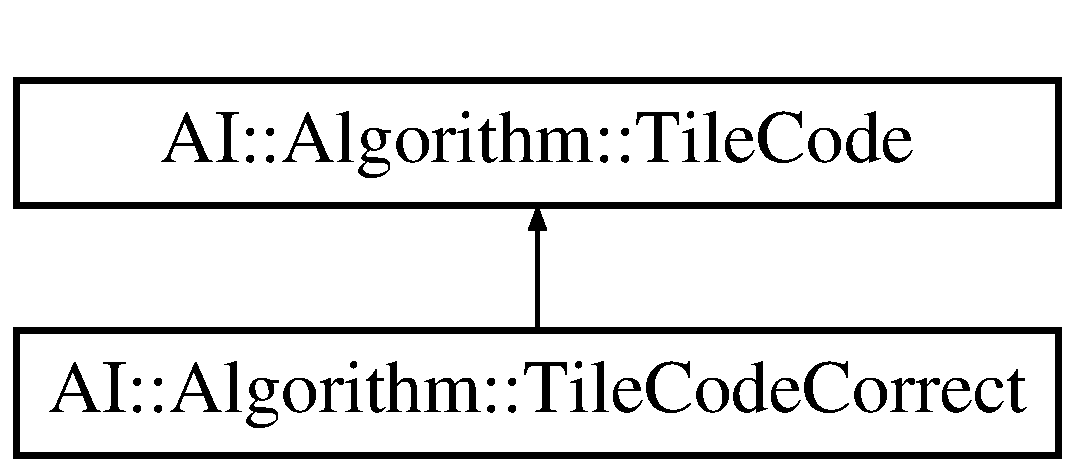
\includegraphics[height=2.000000cm]{classAI_1_1Algorithm_1_1TileCodeCorrect}
\end{center}
\end{figure}
\subsection*{Public Member Functions}
\begin{DoxyCompactItemize}
\item 
\hyperlink{classAI_1_1Algorithm_1_1TileCodeCorrect_a4347bf107c7d252ce0e080be0e134313}{Tile\-Code\-Correct} (vector$<$ \hyperlink{classAI_1_1Algorithm_1_1DimensionInfo}{Dimension\-Info}$<$ F\-L\-O\-A\-T $>$ $>$ dimensional\-Infos, size\-\_\-t num\-Tilings)
\item 
virtual void \hyperlink{classAI_1_1Algorithm_1_1TileCodeCorrect_abb6d45df5a7f6d6263f063586b417eaa}{get\-Feature\-Vector} (const S\-T\-A\-T\-E\-\_\-\-C\-O\-N\-T \&parameters, F\-E\-A\-T\-U\-R\-E\-\_\-\-V\-E\-C\-T\-O\-R \&fv)
\end{DoxyCompactItemize}
\subsection*{Additional Inherited Members}


\subsection{Constructor \& Destructor Documentation}
\hypertarget{classAI_1_1Algorithm_1_1TileCodeCorrect_a4347bf107c7d252ce0e080be0e134313}{\index{A\-I\-::\-Algorithm\-::\-Tile\-Code\-Correct@{A\-I\-::\-Algorithm\-::\-Tile\-Code\-Correct}!Tile\-Code\-Correct@{Tile\-Code\-Correct}}
\index{Tile\-Code\-Correct@{Tile\-Code\-Correct}!AI::Algorithm::TileCodeCorrect@{A\-I\-::\-Algorithm\-::\-Tile\-Code\-Correct}}
\subsubsection[{Tile\-Code\-Correct}]{\setlength{\rightskip}{0pt plus 5cm}A\-I\-::\-Algorithm\-::\-Tile\-Code\-Correct\-::\-Tile\-Code\-Correct (
\begin{DoxyParamCaption}
\item[{vector$<$ {\bf Dimension\-Info}$<$ F\-L\-O\-A\-T $>$ $>$}]{dimensional\-Infos, }
\item[{size\-\_\-t}]{num\-Tilings}
\end{DoxyParamCaption}
)\hspace{0.3cm}{\ttfamily [inline]}}}\label{classAI_1_1Algorithm_1_1TileCodeCorrect_a4347bf107c7d252ce0e080be0e134313}

\begin{DoxyParams}{Parameters}
{\em dimensional\-Infos} & A vector dimensional\-Infos. \\
\hline
{\em num\-Tilings} & The higher the value, the more accurate is the generalization. \\
\hline
\end{DoxyParams}


\subsection{Member Function Documentation}
\hypertarget{classAI_1_1Algorithm_1_1TileCodeCorrect_abb6d45df5a7f6d6263f063586b417eaa}{\index{A\-I\-::\-Algorithm\-::\-Tile\-Code\-Correct@{A\-I\-::\-Algorithm\-::\-Tile\-Code\-Correct}!get\-Feature\-Vector@{get\-Feature\-Vector}}
\index{get\-Feature\-Vector@{get\-Feature\-Vector}!AI::Algorithm::TileCodeCorrect@{A\-I\-::\-Algorithm\-::\-Tile\-Code\-Correct}}
\subsubsection[{get\-Feature\-Vector}]{\setlength{\rightskip}{0pt plus 5cm}void A\-I\-::\-Algorithm\-::\-Tile\-Code\-Correct\-::get\-Feature\-Vector (
\begin{DoxyParamCaption}
\item[{const S\-T\-A\-T\-E\-\_\-\-C\-O\-N\-T \&}]{parameters, }
\item[{F\-E\-A\-T\-U\-R\-E\-\_\-\-V\-E\-C\-T\-O\-R \&}]{fv}
\end{DoxyParamCaption}
)\hspace{0.3cm}{\ttfamily [inline]}, {\ttfamily [virtual]}}}\label{classAI_1_1Algorithm_1_1TileCodeCorrect_abb6d45df5a7f6d6263f063586b417eaa}
Hashed the parameter in Real space to a Natural space \mbox{[}0, infinity). 
\begin{DoxyParams}{Parameters}
{\em parameters} & \\
\hline
\end{DoxyParams}
\begin{DoxyReturn}{Returns}
Vector of discretize index. 
\end{DoxyReturn}


Implements \hyperlink{classAI_1_1Algorithm_1_1TileCode_ad2ba639c550e7d267d066e54b20f6000}{A\-I\-::\-Algorithm\-::\-Tile\-Code}.



The documentation for this class was generated from the following file\-:\begin{DoxyCompactItemize}
\item 
Algorithms/\-Supervised\-Learning/Tile\-Code\-Correct.\-h\end{DoxyCompactItemize}

\hypertarget{classAI_1_1Algorithm_1_1TileCodeMt1993764}{\section{A\+I\+:\+:Algorithm\+:\+:Tile\+Code\+Mt1993764 Class Reference}
\label{classAI_1_1Algorithm_1_1TileCodeMt1993764}\index{A\+I\+::\+Algorithm\+::\+Tile\+Code\+Mt1993764@{A\+I\+::\+Algorithm\+::\+Tile\+Code\+Mt1993764}}
}


Tile Code using Mt1993764 hash.\+2.  




{\ttfamily \#include $<$Tile\+Code\+Mt1993764.\+h$>$}

Inheritance diagram for A\+I\+:\+:Algorithm\+:\+:Tile\+Code\+Mt1993764\+:\begin{figure}[H]
\begin{center}
\leavevmode
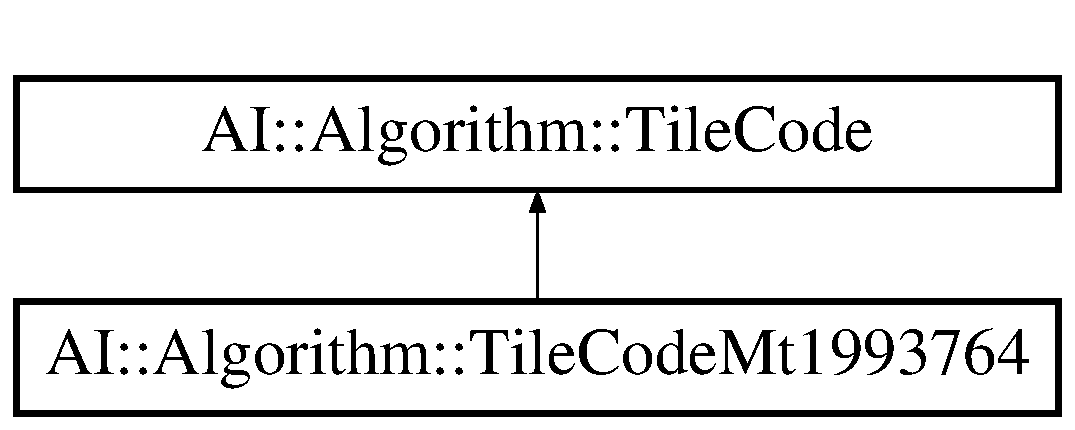
\includegraphics[height=2.000000cm]{classAI_1_1Algorithm_1_1TileCodeMt1993764}
\end{center}
\end{figure}
\subsection*{Public Member Functions}
\begin{DoxyCompactItemize}
\item 
\hyperlink{classAI_1_1Algorithm_1_1TileCodeMt1993764_a0d8eee3e74ccf5587d1f376e9c54a33f}{Tile\+Code\+Mt1993764} (vector$<$ \hyperlink{classAI_1_1Algorithm_1_1DimensionInfo}{Dimension\+Info}$<$ \hyperlink{namespaceAI_a41b74884a20833db653dded3918e05c3}{F\+L\+O\+A\+T} $>$ $>$ dimensional\+Infos, size\+\_\+t num\+Tilings)
\item 
\hyperlink{classAI_1_1Algorithm_1_1TileCodeMt1993764_a6062251f25cab695518db0fda5f97dc6}{Tile\+Code\+Mt1993764} (vector$<$ \hyperlink{classAI_1_1Algorithm_1_1DimensionInfo}{Dimension\+Info}$<$ \hyperlink{namespaceAI_a41b74884a20833db653dded3918e05c3}{F\+L\+O\+A\+T} $>$ $>$ dimensional\+Infos, size\+\_\+t num\+Tilings, size\+\_\+t size\+Hint)
\item 
virtual void \hyperlink{classAI_1_1Algorithm_1_1TileCodeMt1993764_a8d3e8fd183947d9dcb19e63139ea0871}{get\+Feature\+Vector} (const \hyperlink{namespaceAI_aff63ec21d97dd5f086fddbc3103f5707}{S\+T\+A\+T\+E\+\_\+\+C\+O\+N\+T} \&parameters, \hyperlink{namespaceAI_a23a39e1b301a5c1345fa508796940631}{F\+E\+A\+T\+U\+R\+E\+\_\+\+V\+E\+C\+T\+O\+R} \&fv)
\end{DoxyCompactItemize}
\subsection*{Protected Attributes}
\begin{DoxyCompactItemize}
\item 
\hypertarget{classAI_1_1Algorithm_1_1TileCodeMt1993764_a2b2f796c8f67e2076c1149c9d5e43be9}{std\+::mt19937\+\_\+64 {\bfseries \+\_\+prng}}\label{classAI_1_1Algorithm_1_1TileCodeMt1993764_a2b2f796c8f67e2076c1149c9d5e43be9}

\end{DoxyCompactItemize}
\subsection*{Additional Inherited Members}


\subsection{Detailed Description}
Tile Code using Mt1993764 hash.\+2. 

\subsection{Constructor \& Destructor Documentation}
\hypertarget{classAI_1_1Algorithm_1_1TileCodeMt1993764_a0d8eee3e74ccf5587d1f376e9c54a33f}{\index{A\+I\+::\+Algorithm\+::\+Tile\+Code\+Mt1993764@{A\+I\+::\+Algorithm\+::\+Tile\+Code\+Mt1993764}!Tile\+Code\+Mt1993764@{Tile\+Code\+Mt1993764}}
\index{Tile\+Code\+Mt1993764@{Tile\+Code\+Mt1993764}!A\+I\+::\+Algorithm\+::\+Tile\+Code\+Mt1993764@{A\+I\+::\+Algorithm\+::\+Tile\+Code\+Mt1993764}}
\subsubsection[{Tile\+Code\+Mt1993764}]{\setlength{\rightskip}{0pt plus 5cm}A\+I\+::\+Algorithm\+::\+Tile\+Code\+Mt1993764\+::\+Tile\+Code\+Mt1993764 (
\begin{DoxyParamCaption}
\item[{vector$<$ {\bf Dimension\+Info}$<$ {\bf F\+L\+O\+A\+T} $>$ $>$}]{dimensional\+Infos, }
\item[{size\+\_\+t}]{num\+Tilings}
\end{DoxyParamCaption}
)\hspace{0.3cm}{\ttfamily [inline]}}}\label{classAI_1_1Algorithm_1_1TileCodeMt1993764_a0d8eee3e74ccf5587d1f376e9c54a33f}

\begin{DoxyParams}{Parameters}
{\em dimensional\+Infos} & \\
\hline
{\em num\+Tilings} & \\
\hline
\end{DoxyParams}
\hypertarget{classAI_1_1Algorithm_1_1TileCodeMt1993764_a6062251f25cab695518db0fda5f97dc6}{\index{A\+I\+::\+Algorithm\+::\+Tile\+Code\+Mt1993764@{A\+I\+::\+Algorithm\+::\+Tile\+Code\+Mt1993764}!Tile\+Code\+Mt1993764@{Tile\+Code\+Mt1993764}}
\index{Tile\+Code\+Mt1993764@{Tile\+Code\+Mt1993764}!A\+I\+::\+Algorithm\+::\+Tile\+Code\+Mt1993764@{A\+I\+::\+Algorithm\+::\+Tile\+Code\+Mt1993764}}
\subsubsection[{Tile\+Code\+Mt1993764}]{\setlength{\rightskip}{0pt plus 5cm}A\+I\+::\+Algorithm\+::\+Tile\+Code\+Mt1993764\+::\+Tile\+Code\+Mt1993764 (
\begin{DoxyParamCaption}
\item[{vector$<$ {\bf Dimension\+Info}$<$ {\bf F\+L\+O\+A\+T} $>$ $>$}]{dimensional\+Infos, }
\item[{size\+\_\+t}]{num\+Tilings, }
\item[{size\+\_\+t}]{size\+Hint}
\end{DoxyParamCaption}
)\hspace{0.3cm}{\ttfamily [inline]}}}\label{classAI_1_1Algorithm_1_1TileCodeMt1993764_a6062251f25cab695518db0fda5f97dc6}

\begin{DoxyParams}{Parameters}
{\em dimensional\+Infos} & \\
\hline
{\em num\+Tilings} & \\
\hline
{\em size\+Hint} & If size\+Hint is greater than calculated size, then size\+Hint will be used instead. The bigger the size\+Hint, the less likely is the collision during hashing. \\
\hline
\end{DoxyParams}


\subsection{Member Function Documentation}
\hypertarget{classAI_1_1Algorithm_1_1TileCodeMt1993764_a8d3e8fd183947d9dcb19e63139ea0871}{\index{A\+I\+::\+Algorithm\+::\+Tile\+Code\+Mt1993764@{A\+I\+::\+Algorithm\+::\+Tile\+Code\+Mt1993764}!get\+Feature\+Vector@{get\+Feature\+Vector}}
\index{get\+Feature\+Vector@{get\+Feature\+Vector}!A\+I\+::\+Algorithm\+::\+Tile\+Code\+Mt1993764@{A\+I\+::\+Algorithm\+::\+Tile\+Code\+Mt1993764}}
\subsubsection[{get\+Feature\+Vector}]{\setlength{\rightskip}{0pt plus 5cm}void A\+I\+::\+Algorithm\+::\+Tile\+Code\+Mt1993764\+::get\+Feature\+Vector (
\begin{DoxyParamCaption}
\item[{const {\bf S\+T\+A\+T\+E\+\_\+\+C\+O\+N\+T} \&}]{parameters, }
\item[{{\bf F\+E\+A\+T\+U\+R\+E\+\_\+\+V\+E\+C\+T\+O\+R} \&}]{fv}
\end{DoxyParamCaption}
)\hspace{0.3cm}{\ttfamily [inline]}, {\ttfamily [virtual]}}}\label{classAI_1_1Algorithm_1_1TileCodeMt1993764_a8d3e8fd183947d9dcb19e63139ea0871}
Hashed the parameter in Real space to a Natural space \mbox{[}0, infinity). 
\begin{DoxyParams}{Parameters}
{\em parameters} & \\
\hline
\end{DoxyParams}
\begin{DoxyReturn}{Returns}
Vector of discretize index. 
\end{DoxyReturn}


Implements \hyperlink{classAI_1_1Algorithm_1_1TileCode_ad2ba639c550e7d267d066e54b20f6000}{A\+I\+::\+Algorithm\+::\+Tile\+Code}.



The documentation for this class was generated from the following file\+:\begin{DoxyCompactItemize}
\item 
Algorithms/\+Supervised\+Learning/Tile\+Code\+Mt1993764.\+h\end{DoxyCompactItemize}

\hypertarget{classAI_1_1Algorithm_1_1TileCodeMurMur}{\section{A\-I\-:\-:Algorithm\-:\-:Tile\-Code\-Mur\-Mur Class Reference}
\label{classAI_1_1Algorithm_1_1TileCodeMurMur}\index{A\-I\-::\-Algorithm\-::\-Tile\-Code\-Mur\-Mur@{A\-I\-::\-Algorithm\-::\-Tile\-Code\-Mur\-Mur}}
}
Inheritance diagram for A\-I\-:\-:Algorithm\-:\-:Tile\-Code\-Mur\-Mur\-:\begin{figure}[H]
\begin{center}
\leavevmode
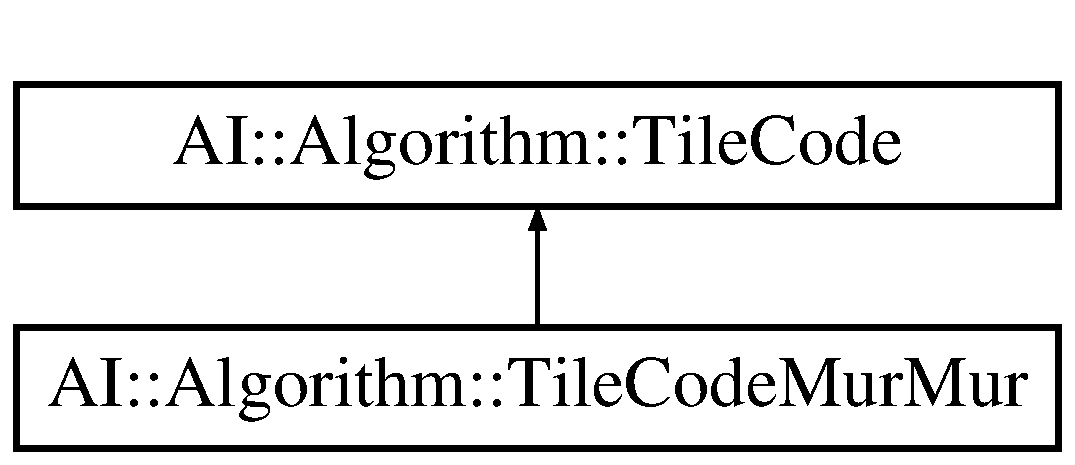
\includegraphics[height=2.000000cm]{classAI_1_1Algorithm_1_1TileCodeMurMur}
\end{center}
\end{figure}
\subsection*{Public Member Functions}
\begin{DoxyCompactItemize}
\item 
\hypertarget{classAI_1_1Algorithm_1_1TileCodeMurMur_a48746c4faa0e887b4a1fb16aba0cd6d9}{{\bfseries Tile\-Code\-Mur\-Mur} (vector$<$ \hyperlink{classAI_1_1Algorithm_1_1DimensionInfo}{Dimension\-Info}$<$ F\-L\-O\-A\-T $>$ $>$ dimensional\-Infos, size\-\_\-t num\-Tilings)}\label{classAI_1_1Algorithm_1_1TileCodeMurMur_a48746c4faa0e887b4a1fb16aba0cd6d9}

\item 
\hypertarget{classAI_1_1Algorithm_1_1TileCodeMurMur_a55c39ff49b9686a90ed6f823986fe4c3}{{\bfseries Tile\-Code\-Mur\-Mur} (vector$<$ \hyperlink{classAI_1_1Algorithm_1_1DimensionInfo}{Dimension\-Info}$<$ F\-L\-O\-A\-T $>$ $>$ dimensional\-Infos, size\-\_\-t num\-Tilings, size\-\_\-t size\-Hint)}\label{classAI_1_1Algorithm_1_1TileCodeMurMur_a55c39ff49b9686a90ed6f823986fe4c3}

\item 
virtual void \hyperlink{classAI_1_1Algorithm_1_1TileCodeMurMur_abd19bfe7dd3ddace0cec0ad9a8715392}{get\-Feature\-Vector} (const S\-T\-A\-T\-E\-\_\-\-C\-O\-N\-T \&parameters, F\-E\-A\-T\-U\-R\-E\-\_\-\-V\-E\-C\-T\-O\-R \&fv)
\end{DoxyCompactItemize}
\subsection*{Additional Inherited Members}


\subsection{Member Function Documentation}
\hypertarget{classAI_1_1Algorithm_1_1TileCodeMurMur_abd19bfe7dd3ddace0cec0ad9a8715392}{\index{A\-I\-::\-Algorithm\-::\-Tile\-Code\-Mur\-Mur@{A\-I\-::\-Algorithm\-::\-Tile\-Code\-Mur\-Mur}!get\-Feature\-Vector@{get\-Feature\-Vector}}
\index{get\-Feature\-Vector@{get\-Feature\-Vector}!AI::Algorithm::TileCodeMurMur@{A\-I\-::\-Algorithm\-::\-Tile\-Code\-Mur\-Mur}}
\subsubsection[{get\-Feature\-Vector}]{\setlength{\rightskip}{0pt plus 5cm}void A\-I\-::\-Algorithm\-::\-Tile\-Code\-Mur\-Mur\-::get\-Feature\-Vector (
\begin{DoxyParamCaption}
\item[{const S\-T\-A\-T\-E\-\_\-\-C\-O\-N\-T \&}]{parameters, }
\item[{F\-E\-A\-T\-U\-R\-E\-\_\-\-V\-E\-C\-T\-O\-R \&}]{fv}
\end{DoxyParamCaption}
)\hspace{0.3cm}{\ttfamily [inline]}, {\ttfamily [virtual]}}}\label{classAI_1_1Algorithm_1_1TileCodeMurMur_abd19bfe7dd3ddace0cec0ad9a8715392}
Hashed the parameter in Real space to a Natural space \mbox{[}0, infinity). 
\begin{DoxyParams}{Parameters}
{\em parameters} & \\
\hline
\end{DoxyParams}
\begin{DoxyReturn}{Returns}
Vector of discretize index. 
\end{DoxyReturn}


Implements \hyperlink{classAI_1_1Algorithm_1_1TileCode_ad2ba639c550e7d267d066e54b20f6000}{A\-I\-::\-Algorithm\-::\-Tile\-Code}.



The documentation for this class was generated from the following file\-:\begin{DoxyCompactItemize}
\item 
Algorithms/\-Supervised\-Learning/Tile\-Code\-Mur\-Mur.\-h\end{DoxyCompactItemize}

\hypertarget{classAI_1_1Algorithm_1_1TileCodeSuperFastHash}{\section{A\-I\-:\-:Algorithm\-:\-:Tile\-Code\-Super\-Fast\-Hash Class Reference}
\label{classAI_1_1Algorithm_1_1TileCodeSuperFastHash}\index{A\-I\-::\-Algorithm\-::\-Tile\-Code\-Super\-Fast\-Hash@{A\-I\-::\-Algorithm\-::\-Tile\-Code\-Super\-Fast\-Hash}}
}


{\ttfamily \#include $<$Tile\-Code\-Super\-Fast\-Hash.\-h$>$}

Inheritance diagram for A\-I\-:\-:Algorithm\-:\-:Tile\-Code\-Super\-Fast\-Hash\-:\begin{figure}[H]
\begin{center}
\leavevmode
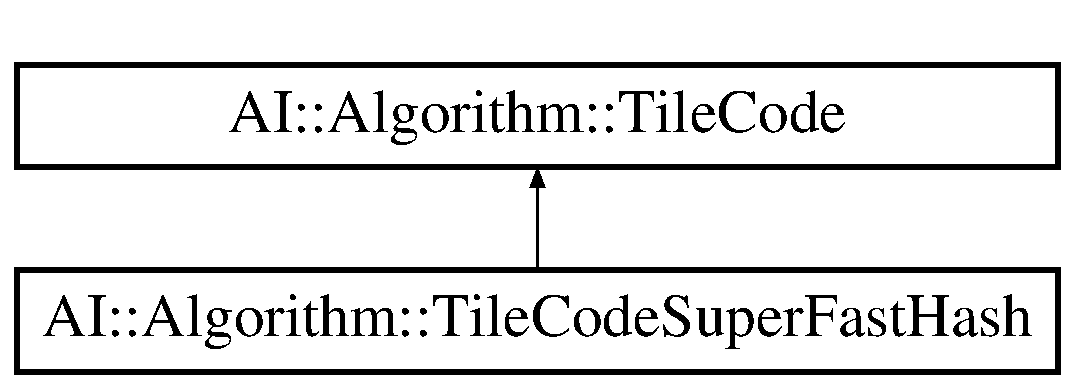
\includegraphics[height=2.000000cm]{classAI_1_1Algorithm_1_1TileCodeSuperFastHash}
\end{center}
\end{figure}
\subsection*{Public Member Functions}
\begin{DoxyCompactItemize}
\item 
\hyperlink{classAI_1_1Algorithm_1_1TileCodeSuperFastHash_a7538ed36cf8ae0a15ff4c902a335266b}{Tile\-Code\-Super\-Fast\-Hash} (vector$<$ \hyperlink{classAI_1_1Algorithm_1_1DimensionInfo}{Dimension\-Info}$<$ \hyperlink{namespaceAI_a41b74884a20833db653dded3918e05c3}{F\-L\-O\-A\-T} $>$ $>$ dimensional\-Infos, size\-\_\-t num\-Tilings)
\item 
\hyperlink{classAI_1_1Algorithm_1_1TileCodeSuperFastHash_a724f6d6f40f0f8f2e4d4692eb3f6c09f}{Tile\-Code\-Super\-Fast\-Hash} (vector$<$ \hyperlink{classAI_1_1Algorithm_1_1DimensionInfo}{Dimension\-Info}$<$ \hyperlink{namespaceAI_a41b74884a20833db653dded3918e05c3}{F\-L\-O\-A\-T} $>$ $>$ dimensional\-Infos, size\-\_\-t num\-Tilings, size\-\_\-t size\-Hint)
\item 
virtual void \hyperlink{classAI_1_1Algorithm_1_1TileCodeSuperFastHash_a46f0df02799eb67bc8fb574b265e7e67}{get\-Feature\-Vector} (const \hyperlink{namespaceAI_aff63ec21d97dd5f086fddbc3103f5707}{S\-T\-A\-T\-E\-\_\-\-C\-O\-N\-T} \&parameters, \hyperlink{namespaceAI_a23a39e1b301a5c1345fa508796940631}{F\-E\-A\-T\-U\-R\-E\-\_\-\-V\-E\-C\-T\-O\-R} \&fv)
\end{DoxyCompactItemize}
\subsection*{Additional Inherited Members}


\subsection{Detailed Description}
Tile\-Coding with Superfast hash. Superfast hash created by Paul Hsieh. 

\subsection{Constructor \& Destructor Documentation}
\hypertarget{classAI_1_1Algorithm_1_1TileCodeSuperFastHash_a7538ed36cf8ae0a15ff4c902a335266b}{\index{A\-I\-::\-Algorithm\-::\-Tile\-Code\-Super\-Fast\-Hash@{A\-I\-::\-Algorithm\-::\-Tile\-Code\-Super\-Fast\-Hash}!Tile\-Code\-Super\-Fast\-Hash@{Tile\-Code\-Super\-Fast\-Hash}}
\index{Tile\-Code\-Super\-Fast\-Hash@{Tile\-Code\-Super\-Fast\-Hash}!AI::Algorithm::TileCodeSuperFastHash@{A\-I\-::\-Algorithm\-::\-Tile\-Code\-Super\-Fast\-Hash}}
\subsubsection[{Tile\-Code\-Super\-Fast\-Hash}]{\setlength{\rightskip}{0pt plus 5cm}A\-I\-::\-Algorithm\-::\-Tile\-Code\-Super\-Fast\-Hash\-::\-Tile\-Code\-Super\-Fast\-Hash (
\begin{DoxyParamCaption}
\item[{vector$<$ {\bf Dimension\-Info}$<$ {\bf F\-L\-O\-A\-T} $>$ $>$}]{dimensional\-Infos, }
\item[{size\-\_\-t}]{num\-Tilings}
\end{DoxyParamCaption}
)\hspace{0.3cm}{\ttfamily [inline]}}}\label{classAI_1_1Algorithm_1_1TileCodeSuperFastHash_a7538ed36cf8ae0a15ff4c902a335266b}

\begin{DoxyParams}{Parameters}
{\em dimensional\-Infos} & \\
\hline
{\em num\-Tilings} & \\
\hline
\end{DoxyParams}
\hypertarget{classAI_1_1Algorithm_1_1TileCodeSuperFastHash_a724f6d6f40f0f8f2e4d4692eb3f6c09f}{\index{A\-I\-::\-Algorithm\-::\-Tile\-Code\-Super\-Fast\-Hash@{A\-I\-::\-Algorithm\-::\-Tile\-Code\-Super\-Fast\-Hash}!Tile\-Code\-Super\-Fast\-Hash@{Tile\-Code\-Super\-Fast\-Hash}}
\index{Tile\-Code\-Super\-Fast\-Hash@{Tile\-Code\-Super\-Fast\-Hash}!AI::Algorithm::TileCodeSuperFastHash@{A\-I\-::\-Algorithm\-::\-Tile\-Code\-Super\-Fast\-Hash}}
\subsubsection[{Tile\-Code\-Super\-Fast\-Hash}]{\setlength{\rightskip}{0pt plus 5cm}A\-I\-::\-Algorithm\-::\-Tile\-Code\-Super\-Fast\-Hash\-::\-Tile\-Code\-Super\-Fast\-Hash (
\begin{DoxyParamCaption}
\item[{vector$<$ {\bf Dimension\-Info}$<$ {\bf F\-L\-O\-A\-T} $>$ $>$}]{dimensional\-Infos, }
\item[{size\-\_\-t}]{num\-Tilings, }
\item[{size\-\_\-t}]{size\-Hint}
\end{DoxyParamCaption}
)\hspace{0.3cm}{\ttfamily [inline]}}}\label{classAI_1_1Algorithm_1_1TileCodeSuperFastHash_a724f6d6f40f0f8f2e4d4692eb3f6c09f}

\begin{DoxyParams}{Parameters}
{\em dimensional\-Infos} & \\
\hline
{\em num\-Tilings} & \\
\hline
{\em size\-Hint} & If size\-Hint is greater than calculated size, then size\-Hint will be used instead. The bigger the size\-Hint, the less likely is the collision during hashing. \\
\hline
\end{DoxyParams}


\subsection{Member Function Documentation}
\hypertarget{classAI_1_1Algorithm_1_1TileCodeSuperFastHash_a46f0df02799eb67bc8fb574b265e7e67}{\index{A\-I\-::\-Algorithm\-::\-Tile\-Code\-Super\-Fast\-Hash@{A\-I\-::\-Algorithm\-::\-Tile\-Code\-Super\-Fast\-Hash}!get\-Feature\-Vector@{get\-Feature\-Vector}}
\index{get\-Feature\-Vector@{get\-Feature\-Vector}!AI::Algorithm::TileCodeSuperFastHash@{A\-I\-::\-Algorithm\-::\-Tile\-Code\-Super\-Fast\-Hash}}
\subsubsection[{get\-Feature\-Vector}]{\setlength{\rightskip}{0pt plus 5cm}void A\-I\-::\-Algorithm\-::\-Tile\-Code\-Super\-Fast\-Hash\-::get\-Feature\-Vector (
\begin{DoxyParamCaption}
\item[{const {\bf S\-T\-A\-T\-E\-\_\-\-C\-O\-N\-T} \&}]{parameters, }
\item[{{\bf F\-E\-A\-T\-U\-R\-E\-\_\-\-V\-E\-C\-T\-O\-R} \&}]{fv}
\end{DoxyParamCaption}
)\hspace{0.3cm}{\ttfamily [inline]}, {\ttfamily [virtual]}}}\label{classAI_1_1Algorithm_1_1TileCodeSuperFastHash_a46f0df02799eb67bc8fb574b265e7e67}
Hashed the parameter in Real space to a Natural space \mbox{[}0, infinity). 
\begin{DoxyParams}{Parameters}
{\em parameters} & \\
\hline
\end{DoxyParams}
\begin{DoxyReturn}{Returns}
Vector of discretize index. 
\end{DoxyReturn}


Implements \hyperlink{classAI_1_1Algorithm_1_1TileCode_ad2ba639c550e7d267d066e54b20f6000}{A\-I\-::\-Algorithm\-::\-Tile\-Code}.



The documentation for this class was generated from the following file\-:\begin{DoxyCompactItemize}
\item 
Algorithms/\-Supervised\-Learning/Tile\-Code\-Super\-Fast\-Hash.\-h\end{DoxyCompactItemize}

\hypertarget{classAI_1_1Algorithm_1_1TileCodeUNH}{\section{A\-I\-:\-:Algorithm\-:\-:Tile\-Code\-U\-N\-H Class Reference}
\label{classAI_1_1Algorithm_1_1TileCodeUNH}\index{A\-I\-::\-Algorithm\-::\-Tile\-Code\-U\-N\-H@{A\-I\-::\-Algorithm\-::\-Tile\-Code\-U\-N\-H}}
}
Inheritance diagram for A\-I\-:\-:Algorithm\-:\-:Tile\-Code\-U\-N\-H\-:\begin{figure}[H]
\begin{center}
\leavevmode
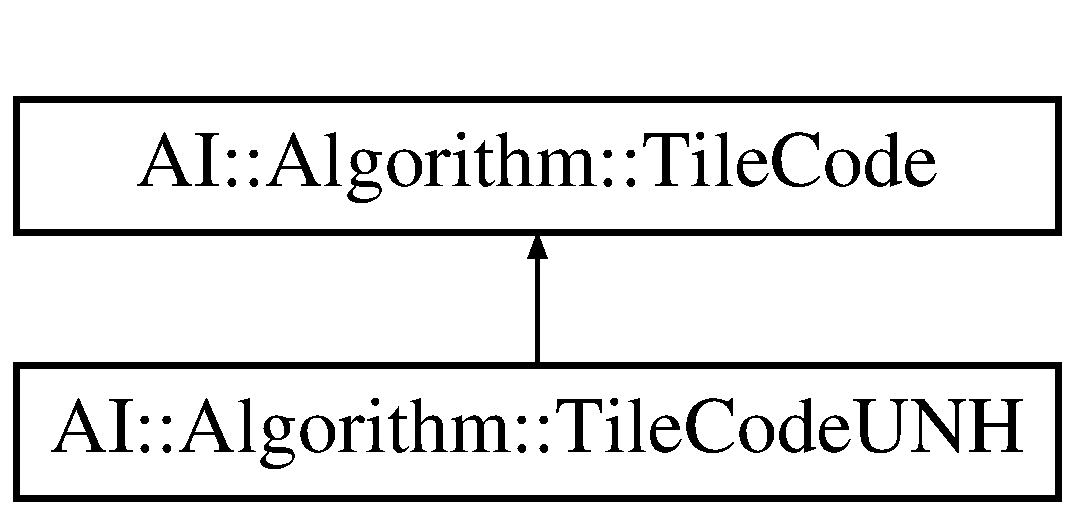
\includegraphics[height=2.000000cm]{classAI_1_1Algorithm_1_1TileCodeUNH}
\end{center}
\end{figure}
\subsection*{Public Member Functions}
\begin{DoxyCompactItemize}
\item 
\hypertarget{classAI_1_1Algorithm_1_1TileCodeUNH_abcbd8f8e4bcc48dda33a9e98a012fa5d}{{\bfseries Tile\-Code\-U\-N\-H} (vector$<$ \hyperlink{classAI_1_1Algorithm_1_1DimensionInfo}{Dimension\-Info}$<$ F\-L\-O\-A\-T $>$ $>$ dimensional\-Infos, size\-\_\-t num\-Tilings)}\label{classAI_1_1Algorithm_1_1TileCodeUNH_abcbd8f8e4bcc48dda33a9e98a012fa5d}

\item 
\hypertarget{classAI_1_1Algorithm_1_1TileCodeUNH_ac6d35486b3f5e94a6a6d95dd4a5e1e14}{{\bfseries Tile\-Code\-U\-N\-H} (vector$<$ \hyperlink{classAI_1_1Algorithm_1_1DimensionInfo}{Dimension\-Info}$<$ F\-L\-O\-A\-T $>$ $>$ dimensional\-Infos, size\-\_\-t num\-Tilings, size\-\_\-t size\-Hint)}\label{classAI_1_1Algorithm_1_1TileCodeUNH_ac6d35486b3f5e94a6a6d95dd4a5e1e14}

\item 
virtual void \hyperlink{classAI_1_1Algorithm_1_1TileCodeUNH_a7b13840ff09b20ff2ad06965f3f4800f}{get\-Feature\-Vector} (const S\-T\-A\-T\-E\-\_\-\-C\-O\-N\-T \&parameters, F\-E\-A\-T\-U\-R\-E\-\_\-\-V\-E\-C\-T\-O\-R \&fv)
\item 
\hypertarget{classAI_1_1Algorithm_1_1TileCodeUNH_a02daa0818beff76016b3d000a2c86b68}{size\-\_\-t {\bfseries mod} (size\-\_\-t n, size\-\_\-t k)}\label{classAI_1_1Algorithm_1_1TileCodeUNH_a02daa0818beff76016b3d000a2c86b68}

\end{DoxyCompactItemize}
\subsection*{Protected Attributes}
\begin{DoxyCompactItemize}
\item 
\hypertarget{classAI_1_1Algorithm_1_1TileCodeUNH_aeab9b9508b1d9985bd5f543aa7cfbc82}{vector$<$ A\-I\-::\-F\-L\-O\-A\-T $>$ {\bfseries \-\_\-normalization}}\label{classAI_1_1Algorithm_1_1TileCodeUNH_aeab9b9508b1d9985bd5f543aa7cfbc82}

\end{DoxyCompactItemize}
\subsection*{Additional Inherited Members}


\subsection{Member Function Documentation}
\hypertarget{classAI_1_1Algorithm_1_1TileCodeUNH_a7b13840ff09b20ff2ad06965f3f4800f}{\index{A\-I\-::\-Algorithm\-::\-Tile\-Code\-U\-N\-H@{A\-I\-::\-Algorithm\-::\-Tile\-Code\-U\-N\-H}!get\-Feature\-Vector@{get\-Feature\-Vector}}
\index{get\-Feature\-Vector@{get\-Feature\-Vector}!AI::Algorithm::TileCodeUNH@{A\-I\-::\-Algorithm\-::\-Tile\-Code\-U\-N\-H}}
\subsubsection[{get\-Feature\-Vector}]{\setlength{\rightskip}{0pt plus 5cm}void A\-I\-::\-Algorithm\-::\-Tile\-Code\-U\-N\-H\-::get\-Feature\-Vector (
\begin{DoxyParamCaption}
\item[{const S\-T\-A\-T\-E\-\_\-\-C\-O\-N\-T \&}]{parameters, }
\item[{F\-E\-A\-T\-U\-R\-E\-\_\-\-V\-E\-C\-T\-O\-R \&}]{fv}
\end{DoxyParamCaption}
)\hspace{0.3cm}{\ttfamily [inline]}, {\ttfamily [virtual]}}}\label{classAI_1_1Algorithm_1_1TileCodeUNH_a7b13840ff09b20ff2ad06965f3f4800f}
Hashed the parameter in Real space to a Natural space \mbox{[}0, infinity). 
\begin{DoxyParams}{Parameters}
{\em parameters} & \\
\hline
\end{DoxyParams}
\begin{DoxyReturn}{Returns}
Vector of discretize index. 
\end{DoxyReturn}


Implements \hyperlink{classAI_1_1Algorithm_1_1TileCode_ad2ba639c550e7d267d066e54b20f6000}{A\-I\-::\-Algorithm\-::\-Tile\-Code}.



The documentation for this class was generated from the following file\-:\begin{DoxyCompactItemize}
\item 
Algorithms/\-Supervised\-Learning/Tile\-Code\-U\-N\-H.\-h\end{DoxyCompactItemize}

\hypertarget{classAI_1_1Algorithm_1_1Hash_1_1UNH}{\section{A\+I\+:\+:Algorithm\+:\+:Hash\+:\+:U\+N\+H Class Reference}
\label{classAI_1_1Algorithm_1_1Hash_1_1UNH}\index{A\+I\+::\+Algorithm\+::\+Hash\+::\+U\+N\+H@{A\+I\+::\+Algorithm\+::\+Hash\+::\+U\+N\+H}}
}


\hyperlink{classAI_1_1Algorithm_1_1Hash_1_1UNH}{U\+N\+H} implementation encapsulation.  




{\ttfamily \#include $<$Hash\+U\+N\+H.\+h$>$}

Inheritance diagram for A\+I\+:\+:Algorithm\+:\+:Hash\+:\+:U\+N\+H\+:\begin{figure}[H]
\begin{center}
\leavevmode
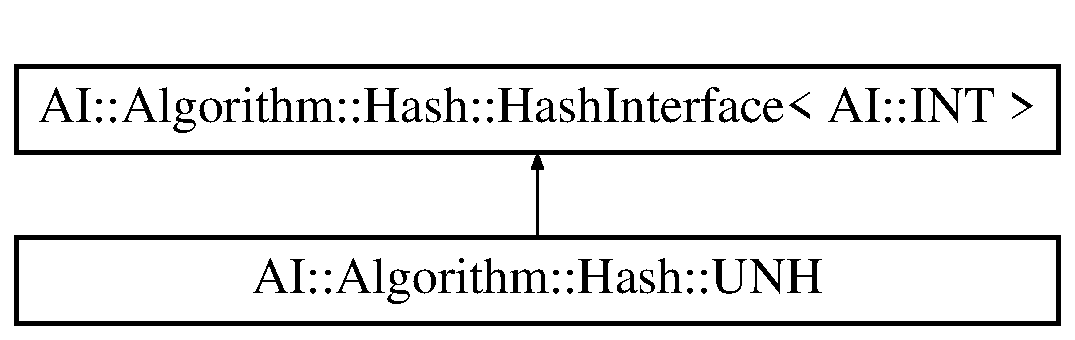
\includegraphics[height=2.000000cm]{classAI_1_1Algorithm_1_1Hash_1_1UNH}
\end{center}
\end{figure}
\subsection*{Public Member Functions}
\begin{DoxyCompactItemize}
\item 
virtual \hyperlink{namespaceAI_ac74584e573f07aa4194b461b1ba7be64}{A\+I\+::\+I\+N\+T} \hyperlink{classAI_1_1Algorithm_1_1Hash_1_1UNH_acc52e3c2f323e748882ee5d9d66be698}{hash} (const \hyperlink{namespaceAI_a9d4bcda82fe0f9aac3c4861e24491581}{A\+I\+::\+B\+Y\+T\+E} $\ast$const byte\+Array, size\+\_\+t len)
\item 
\hypertarget{classAI_1_1Algorithm_1_1Hash_1_1UNH_aacaaa8356755304f4bc1455cf18f16df}{virtual \hyperlink{namespaceAI_ac74584e573f07aa4194b461b1ba7be64}{A\+I\+::\+I\+N\+T} {\bfseries hash} (const vector$<$ \hyperlink{namespaceAI_a9d4bcda82fe0f9aac3c4861e24491581}{A\+I\+::\+B\+Y\+T\+E} $>$ \&byte\+Array)}\label{classAI_1_1Algorithm_1_1Hash_1_1UNH_aacaaa8356755304f4bc1455cf18f16df}

\end{DoxyCompactItemize}


\subsection{Detailed Description}
\hyperlink{classAI_1_1Algorithm_1_1Hash_1_1UNH}{U\+N\+H} implementation encapsulation. 

\subsection{Member Function Documentation}
\hypertarget{classAI_1_1Algorithm_1_1Hash_1_1UNH_acc52e3c2f323e748882ee5d9d66be698}{\index{A\+I\+::\+Algorithm\+::\+Hash\+::\+U\+N\+H@{A\+I\+::\+Algorithm\+::\+Hash\+::\+U\+N\+H}!hash@{hash}}
\index{hash@{hash}!A\+I\+::\+Algorithm\+::\+Hash\+::\+U\+N\+H@{A\+I\+::\+Algorithm\+::\+Hash\+::\+U\+N\+H}}
\subsubsection[{hash}]{\setlength{\rightskip}{0pt plus 5cm}{\bf A\+I\+::\+I\+N\+T} A\+I\+::\+Algorithm\+::\+Hash\+::\+U\+N\+H\+::hash (
\begin{DoxyParamCaption}
\item[{const {\bf A\+I\+::\+B\+Y\+T\+E} $\ast$const}]{byte\+Array, }
\item[{size\+\_\+t}]{len}
\end{DoxyParamCaption}
)\hspace{0.3cm}{\ttfamily [virtual]}}}\label{classAI_1_1Algorithm_1_1Hash_1_1UNH_acc52e3c2f323e748882ee5d9d66be698}

\begin{DoxyParams}{Parameters}
{\em byte\+Array} & \\
\hline
{\em len} & \\
\hline
\end{DoxyParams}
\begin{DoxyReturn}{Returns}
h(byte\+Array) 
\end{DoxyReturn}


Implements \hyperlink{classAI_1_1Algorithm_1_1Hash_1_1HashInterface_ae31d650fd044e3ef372cae18a422e0d9}{A\+I\+::\+Algorithm\+::\+Hash\+::\+Hash\+Interface$<$ A\+I\+::\+I\+N\+T $>$}.



The documentation for this class was generated from the following files\+:\begin{DoxyCompactItemize}
\item 
Algorithms/\+Hash/Hash\+U\+N\+H.\+h\item 
Algorithms/\+Hash/Hash\+U\+N\+H.\+cpp\end{DoxyCompactItemize}

%--- End generated contents ---

% Index
\newpage
\phantomsection
\addcontentsline{toc}{chapter}{Index}
\printindex

\end{document}
